\section{Test case three: three agents $-$ one obstacle}

In this case the initial configurations of the three agents are
$\vect{z}_1$ $=$ $[-6, 3.5, 0]^{\top}$,
$\vect{z}_2$ $=$ $[-6, 2.3, 0]^{\top}$ and
$\vect{z}_3$ $=$ $[-6, 4.7, 0]^{\top}$.
Their desired configurations in steady-state are
$\vect{z}_{1,des}$ $=$ $[6, 3.5, 0]^{\top}$,
$\vect{z}_{2,des}$ $=$ $[6, 2.3, 0]^{\top}$ and
$\vect{z}_{3,des}$ $=$ $[6, 4.7, 0]^{\top}$.
Obstacle $o_1$ is placed between the two at $[0, 3.5]^{\top}$. The penalty
matrices $\mat{Q}$, $\mat{R}$, $\mat{P}$ were set to
$\mat{Q} = 0.5 (I_3 + \dagger_3)$, $\mat{R} = 0.005 I_2$ and
$\mat{P} = 0.5 I_3$, where $\dagger_N$ is a $N \times N$ matrix whose
elements are chosen at random between the values $0.0$ and $1.0$.

In subsection \ref{subsection:d_OFF_trajectories_3_1}, frames of the evolution of the
trajectories of the three agents are depicted. Subsections
\ref{subsection:d_OFF_errors_3_1} and \ref{subsection:d_OFF_inputs_3_1} illustrate
the evolution of the error states and the input signals of the three agents
respectively. Subsection \ref{subsection:d_OFF_distances_3_1} features the
figures relating to the evolution of the distance between the three agents
along with that between them and the obstacle.


%-------------------------------------------------------------------------------
\subsection{Trajectories in 2D}
\label{subsection:d_OFF_trajectories_3_1}

\begin{figure}[H]
  % This file was created by matlab2tikz.
%
%The latest updates can be retrieved from
%  http://www.mathworks.com/matlabcentral/fileexchange/22022-matlab2tikz-matlab2tikz
%where you can also make suggestions and rate matlab2tikz.
%
\definecolor{mycolor1}{rgb}{0.00000,0.44700,0.74100}%
\definecolor{mycolor2}{rgb}{0.85000,0.32500,0.09800}%
\definecolor{mycolor3}{rgb}{0.92900,0.69400,0.12500}%
\definecolor{mycolor4}{rgb}{0.46600,0.67400,0.18800}%
%
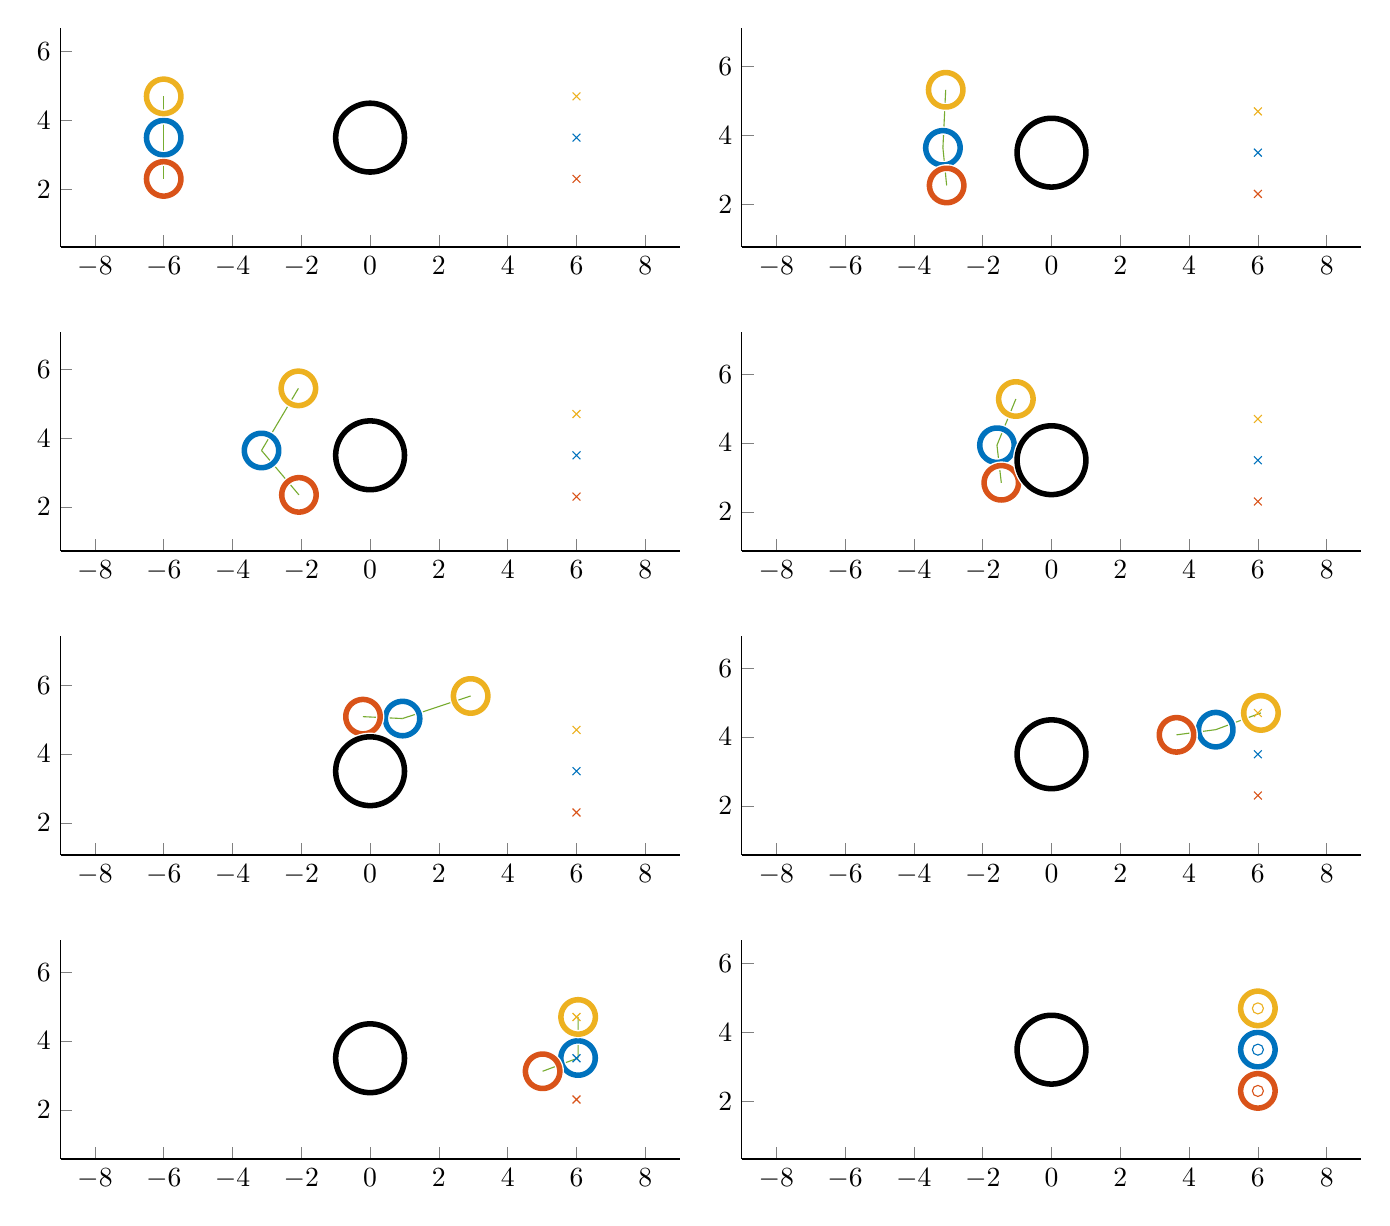
\begin{tikzpicture}

\begin{axis}[%
width=3.096in,
height=1.094in,
at={(2.593in,5.323in)},
scale only axis,
unbounded coords=jump,
xmin=-9,
xmax=9,
ymin=0.318379976997646,
ymax=6.68162002300235,
axis background/.style={fill=white},
axis x line*=bottom,
axis y line*=left
]
\addplot [color=mycolor1,only marks,mark=x,mark options={solid},forget plot]
  table[row sep=crcr]{%
6	3.5\\
};
\addplot [color=mycolor2,only marks,mark=x,mark options={solid},forget plot]
  table[row sep=crcr]{%
6	2.3\\
};
\addplot [color=mycolor3,only marks,mark=x,mark options={solid},forget plot]
  table[row sep=crcr]{%
6	4.7\\
};
\addplot [color=mycolor4,solid,forget plot]
  table[row sep=crcr]{%
-6	3.5\\
-6	2.3\\
};
\addplot [color=mycolor4,solid,forget plot]
  table[row sep=crcr]{%
-6	3.5\\
-6	4.7\\
};
\addplot [color=white,solid,line width=3.0pt,forget plot]
  table[row sep=crcr]{%
-5.5	3.5\\
-5.50030458649045	3.51744974835125\\
-5.50121797487009	3.53487823687206\\
-5.50273905231586	3.55226423163383\\
-5.50486596562921	3.56958655048003\\
-5.5075961234939	3.58682408883347\\
-5.5109261996331	3.60395584540888\\
-5.514852136862	3.62096094779983\\
-5.51936915203084	3.6378186779085\\
-5.52447174185242	3.65450849718747\\
-5.53015368960705	3.67101007166283\\
-5.53640807271661	3.68730329670796\\
-5.5432272711787	3.7033683215379\\
-5.55060297685042	3.71918557339454\\
-5.55852620357054	3.73473578139295\\
-5.56698729810778	3.75\\
-5.57597595192179	3.7649596321166\\
-5.58548121372248	3.77959645173537\\
-5.59549150281253	3.79389262614624\\
-5.60599462319664	3.80783073766283\\
-5.61697777844051	3.82139380484327\\
-5.6284275872613	3.83456530317943\\
-5.64033009983067	3.8473291852295\\
-5.6526708147705	3.85966990016933\\
-5.66543469682057	3.8715724127387\\
-5.67860619515673	3.88302222155949\\
-5.69216926233717	3.89400537680336\\
-5.70610737385376	3.90450849718747\\
-5.72040354826463	3.91451878627752\\
-5.7350403678834	3.92402404807821\\
-5.75	3.93301270189222\\
-5.76526421860705	3.94147379642946\\
-5.78081442660546	3.94939702314958\\
-5.7966316784621	3.9567727288213\\
-5.81269670329204	3.96359192728339\\
-5.82898992833717	3.96984631039295\\
-5.84549150281253	3.97552825814758\\
-5.8621813220915	3.98063084796916\\
-5.87903905220017	3.985147863138\\
-5.89604415459112	3.9890738003669\\
-5.91317591116653	3.9924038765061\\
-5.93041344951997	3.99513403437079\\
-5.94773576836617	3.99726094768414\\
-5.96512176312794	3.99878202512991\\
-5.98255025164875	3.99969541350955\\
-6	4\\
-6.01744974835125	3.99969541350955\\
-6.03487823687206	3.99878202512991\\
-6.05226423163383	3.99726094768414\\
-6.06958655048003	3.99513403437079\\
-6.08682408883347	3.9924038765061\\
-6.10395584540888	3.9890738003669\\
-6.12096094779983	3.985147863138\\
-6.1378186779085	3.98063084796916\\
-6.15450849718747	3.97552825814758\\
-6.17101007166283	3.96984631039295\\
-6.18730329670796	3.96359192728339\\
-6.2033683215379	3.9567727288213\\
-6.21918557339454	3.94939702314958\\
-6.23473578139295	3.94147379642946\\
-6.25	3.93301270189222\\
-6.2649596321166	3.92402404807821\\
-6.27959645173537	3.91451878627752\\
-6.29389262614624	3.90450849718747\\
-6.30783073766283	3.89400537680336\\
-6.32139380484327	3.88302222155949\\
-6.33456530317943	3.8715724127387\\
-6.3473291852295	3.85966990016933\\
-6.35966990016933	3.8473291852295\\
-6.3715724127387	3.83456530317943\\
-6.38302222155949	3.82139380484327\\
-6.39400537680336	3.80783073766283\\
-6.40450849718747	3.79389262614624\\
-6.41451878627752	3.77959645173537\\
-6.42402404807821	3.7649596321166\\
-6.43301270189222	3.75\\
-6.44147379642946	3.73473578139295\\
-6.44939702314958	3.71918557339454\\
-6.4567727288213	3.7033683215379\\
-6.46359192728339	3.68730329670796\\
-6.46984631039295	3.67101007166283\\
-6.47552825814758	3.65450849718747\\
-6.48063084796916	3.6378186779085\\
-6.485147863138	3.62096094779983\\
-6.4890738003669	3.60395584540888\\
-6.4924038765061	3.58682408883347\\
-6.49513403437079	3.56958655048003\\
-6.49726094768414	3.55226423163383\\
-6.49878202512991	3.53487823687206\\
-6.49969541350955	3.51744974835125\\
-6.5	3.5\\
-6.49969541350955	3.48255025164875\\
-6.49878202512991	3.46512176312794\\
-6.49726094768414	3.44773576836617\\
-6.49513403437079	3.43041344951997\\
-6.4924038765061	3.41317591116653\\
-6.4890738003669	3.39604415459112\\
-6.485147863138	3.37903905220017\\
-6.48063084796916	3.3621813220915\\
-6.47552825814758	3.34549150281253\\
-6.46984631039295	3.32898992833717\\
-6.46359192728339	3.31269670329204\\
-6.4567727288213	3.2966316784621\\
-6.44939702314958	3.28081442660546\\
-6.44147379642946	3.26526421860705\\
-6.43301270189222	3.25\\
-6.42402404807821	3.2350403678834\\
-6.41451878627752	3.22040354826463\\
-6.40450849718747	3.20610737385376\\
-6.39400537680336	3.19216926233717\\
-6.38302222155949	3.17860619515673\\
-6.3715724127387	3.16543469682057\\
-6.35966990016933	3.1526708147705\\
-6.3473291852295	3.14033009983067\\
-6.33456530317943	3.1284275872613\\
-6.32139380484327	3.11697777844051\\
-6.30783073766283	3.10599462319664\\
-6.29389262614624	3.09549150281253\\
-6.27959645173537	3.08548121372248\\
-6.2649596321166	3.07597595192179\\
-6.25	3.06698729810778\\
-6.23473578139295	3.05852620357054\\
-6.21918557339454	3.05060297685042\\
-6.2033683215379	3.0432272711787\\
-6.18730329670796	3.03640807271661\\
-6.17101007166283	3.03015368960705\\
-6.15450849718747	3.02447174185242\\
-6.1378186779085	3.01936915203084\\
-6.12096094779983	3.014852136862\\
-6.10395584540888	3.0109261996331\\
-6.08682408883347	3.0075961234939\\
-6.06958655048003	3.00486596562921\\
-6.05226423163383	3.00273905231586\\
-6.03487823687206	3.00121797487009\\
-6.01744974835125	3.00030458649045\\
-6	3\\
-5.98255025164875	3.00030458649045\\
-5.96512176312794	3.00121797487009\\
-5.94773576836617	3.00273905231586\\
-5.93041344951997	3.00486596562921\\
-5.91317591116653	3.0075961234939\\
-5.89604415459112	3.0109261996331\\
-5.87903905220017	3.014852136862\\
-5.8621813220915	3.01936915203084\\
-5.84549150281253	3.02447174185242\\
-5.82898992833717	3.03015368960705\\
-5.81269670329204	3.03640807271661\\
-5.7966316784621	3.0432272711787\\
-5.78081442660546	3.05060297685042\\
-5.76526421860705	3.05852620357054\\
-5.75	3.06698729810778\\
-5.7350403678834	3.07597595192179\\
-5.72040354826463	3.08548121372248\\
-5.70610737385376	3.09549150281253\\
-5.69216926233717	3.10599462319664\\
-5.67860619515673	3.11697777844051\\
-5.66543469682057	3.1284275872613\\
-5.6526708147705	3.14033009983067\\
-5.64033009983067	3.1526708147705\\
-5.6284275872613	3.16543469682057\\
-5.61697777844051	3.17860619515673\\
-5.60599462319664	3.19216926233717\\
-5.59549150281253	3.20610737385376\\
-5.58548121372248	3.22040354826463\\
-5.57597595192179	3.2350403678834\\
-5.56698729810778	3.25\\
-5.55852620357054	3.26526421860705\\
-5.55060297685042	3.28081442660546\\
-5.5432272711787	3.2966316784621\\
-5.53640807271661	3.31269670329204\\
-5.53015368960705	3.32898992833717\\
-5.52447174185242	3.34549150281253\\
-5.51936915203084	3.3621813220915\\
-5.514852136862	3.37903905220017\\
-5.5109261996331	3.39604415459112\\
-5.5075961234939	3.41317591116653\\
-5.50486596562921	3.43041344951997\\
-5.50273905231586	3.44773576836617\\
-5.50121797487009	3.46512176312794\\
-5.50030458649045	3.48255025164875\\
-5.5	3.5\\
nan	nan\\
};
\addplot [color=mycolor1,solid,line width=2.0pt,forget plot]
  table[row sep=crcr]{%
-5.5	3.5\\
-5.50030458649045	3.51744974835125\\
-5.50121797487009	3.53487823687206\\
-5.50273905231586	3.55226423163383\\
-5.50486596562921	3.56958655048003\\
-5.5075961234939	3.58682408883347\\
-5.5109261996331	3.60395584540888\\
-5.514852136862	3.62096094779983\\
-5.51936915203084	3.6378186779085\\
-5.52447174185242	3.65450849718747\\
-5.53015368960705	3.67101007166283\\
-5.53640807271661	3.68730329670796\\
-5.5432272711787	3.7033683215379\\
-5.55060297685042	3.71918557339454\\
-5.55852620357054	3.73473578139295\\
-5.56698729810778	3.75\\
-5.57597595192179	3.7649596321166\\
-5.58548121372248	3.77959645173537\\
-5.59549150281253	3.79389262614624\\
-5.60599462319664	3.80783073766283\\
-5.61697777844051	3.82139380484327\\
-5.6284275872613	3.83456530317943\\
-5.64033009983067	3.8473291852295\\
-5.6526708147705	3.85966990016933\\
-5.66543469682057	3.8715724127387\\
-5.67860619515673	3.88302222155949\\
-5.69216926233717	3.89400537680336\\
-5.70610737385376	3.90450849718747\\
-5.72040354826463	3.91451878627752\\
-5.7350403678834	3.92402404807821\\
-5.75	3.93301270189222\\
-5.76526421860705	3.94147379642946\\
-5.78081442660546	3.94939702314958\\
-5.7966316784621	3.9567727288213\\
-5.81269670329204	3.96359192728339\\
-5.82898992833717	3.96984631039295\\
-5.84549150281253	3.97552825814758\\
-5.8621813220915	3.98063084796916\\
-5.87903905220017	3.985147863138\\
-5.89604415459112	3.9890738003669\\
-5.91317591116653	3.9924038765061\\
-5.93041344951997	3.99513403437079\\
-5.94773576836617	3.99726094768414\\
-5.96512176312794	3.99878202512991\\
-5.98255025164875	3.99969541350955\\
-6	4\\
-6.01744974835125	3.99969541350955\\
-6.03487823687206	3.99878202512991\\
-6.05226423163383	3.99726094768414\\
-6.06958655048003	3.99513403437079\\
-6.08682408883347	3.9924038765061\\
-6.10395584540888	3.9890738003669\\
-6.12096094779983	3.985147863138\\
-6.1378186779085	3.98063084796916\\
-6.15450849718747	3.97552825814758\\
-6.17101007166283	3.96984631039295\\
-6.18730329670796	3.96359192728339\\
-6.2033683215379	3.9567727288213\\
-6.21918557339454	3.94939702314958\\
-6.23473578139295	3.94147379642946\\
-6.25	3.93301270189222\\
-6.2649596321166	3.92402404807821\\
-6.27959645173537	3.91451878627752\\
-6.29389262614624	3.90450849718747\\
-6.30783073766283	3.89400537680336\\
-6.32139380484327	3.88302222155949\\
-6.33456530317943	3.8715724127387\\
-6.3473291852295	3.85966990016933\\
-6.35966990016933	3.8473291852295\\
-6.3715724127387	3.83456530317943\\
-6.38302222155949	3.82139380484327\\
-6.39400537680336	3.80783073766283\\
-6.40450849718747	3.79389262614624\\
-6.41451878627752	3.77959645173537\\
-6.42402404807821	3.7649596321166\\
-6.43301270189222	3.75\\
-6.44147379642946	3.73473578139295\\
-6.44939702314958	3.71918557339454\\
-6.4567727288213	3.7033683215379\\
-6.46359192728339	3.68730329670796\\
-6.46984631039295	3.67101007166283\\
-6.47552825814758	3.65450849718747\\
-6.48063084796916	3.6378186779085\\
-6.485147863138	3.62096094779983\\
-6.4890738003669	3.60395584540888\\
-6.4924038765061	3.58682408883347\\
-6.49513403437079	3.56958655048003\\
-6.49726094768414	3.55226423163383\\
-6.49878202512991	3.53487823687206\\
-6.49969541350955	3.51744974835125\\
-6.5	3.5\\
-6.49969541350955	3.48255025164875\\
-6.49878202512991	3.46512176312794\\
-6.49726094768414	3.44773576836617\\
-6.49513403437079	3.43041344951997\\
-6.4924038765061	3.41317591116653\\
-6.4890738003669	3.39604415459112\\
-6.485147863138	3.37903905220017\\
-6.48063084796916	3.3621813220915\\
-6.47552825814758	3.34549150281253\\
-6.46984631039295	3.32898992833717\\
-6.46359192728339	3.31269670329204\\
-6.4567727288213	3.2966316784621\\
-6.44939702314958	3.28081442660546\\
-6.44147379642946	3.26526421860705\\
-6.43301270189222	3.25\\
-6.42402404807821	3.2350403678834\\
-6.41451878627752	3.22040354826463\\
-6.40450849718747	3.20610737385376\\
-6.39400537680336	3.19216926233717\\
-6.38302222155949	3.17860619515673\\
-6.3715724127387	3.16543469682057\\
-6.35966990016933	3.1526708147705\\
-6.3473291852295	3.14033009983067\\
-6.33456530317943	3.1284275872613\\
-6.32139380484327	3.11697777844051\\
-6.30783073766283	3.10599462319664\\
-6.29389262614624	3.09549150281253\\
-6.27959645173537	3.08548121372248\\
-6.2649596321166	3.07597595192179\\
-6.25	3.06698729810778\\
-6.23473578139295	3.05852620357054\\
-6.21918557339454	3.05060297685042\\
-6.2033683215379	3.0432272711787\\
-6.18730329670796	3.03640807271661\\
-6.17101007166283	3.03015368960705\\
-6.15450849718747	3.02447174185242\\
-6.1378186779085	3.01936915203084\\
-6.12096094779983	3.014852136862\\
-6.10395584540888	3.0109261996331\\
-6.08682408883347	3.0075961234939\\
-6.06958655048003	3.00486596562921\\
-6.05226423163383	3.00273905231586\\
-6.03487823687206	3.00121797487009\\
-6.01744974835125	3.00030458649045\\
-6	3\\
-5.98255025164875	3.00030458649045\\
-5.96512176312794	3.00121797487009\\
-5.94773576836617	3.00273905231586\\
-5.93041344951997	3.00486596562921\\
-5.91317591116653	3.0075961234939\\
-5.89604415459112	3.0109261996331\\
-5.87903905220017	3.014852136862\\
-5.8621813220915	3.01936915203084\\
-5.84549150281253	3.02447174185242\\
-5.82898992833717	3.03015368960705\\
-5.81269670329204	3.03640807271661\\
-5.7966316784621	3.0432272711787\\
-5.78081442660546	3.05060297685042\\
-5.76526421860705	3.05852620357054\\
-5.75	3.06698729810778\\
-5.7350403678834	3.07597595192179\\
-5.72040354826463	3.08548121372248\\
-5.70610737385376	3.09549150281253\\
-5.69216926233717	3.10599462319664\\
-5.67860619515673	3.11697777844051\\
-5.66543469682057	3.1284275872613\\
-5.6526708147705	3.14033009983067\\
-5.64033009983067	3.1526708147705\\
-5.6284275872613	3.16543469682057\\
-5.61697777844051	3.17860619515673\\
-5.60599462319664	3.19216926233717\\
-5.59549150281253	3.20610737385376\\
-5.58548121372248	3.22040354826463\\
-5.57597595192179	3.2350403678834\\
-5.56698729810778	3.25\\
-5.55852620357054	3.26526421860705\\
-5.55060297685042	3.28081442660546\\
-5.5432272711787	3.2966316784621\\
-5.53640807271661	3.31269670329204\\
-5.53015368960705	3.32898992833717\\
-5.52447174185242	3.34549150281253\\
-5.51936915203084	3.3621813220915\\
-5.514852136862	3.37903905220017\\
-5.5109261996331	3.39604415459112\\
-5.5075961234939	3.41317591116653\\
-5.50486596562921	3.43041344951997\\
-5.50273905231586	3.44773576836617\\
-5.50121797487009	3.46512176312794\\
-5.50030458649045	3.48255025164875\\
-5.5	3.5\\
nan	nan\\
};
\addplot [color=white,solid,line width=3.0pt,forget plot]
  table[row sep=crcr]{%
-5.5	2.3\\
-5.50030458649045	2.31744974835125\\
-5.50121797487009	2.33487823687206\\
-5.50273905231586	2.35226423163383\\
-5.50486596562921	2.36958655048003\\
-5.5075961234939	2.38682408883346\\
-5.5109261996331	2.40395584540888\\
-5.514852136862	2.42096094779983\\
-5.51936915203084	2.4378186779085\\
-5.52447174185242	2.45450849718747\\
-5.53015368960705	2.47101007166283\\
-5.53640807271661	2.48730329670796\\
-5.5432272711787	2.5033683215379\\
-5.55060297685042	2.51918557339454\\
-5.55852620357054	2.53473578139295\\
-5.56698729810778	2.55\\
-5.57597595192179	2.5649596321166\\
-5.58548121372248	2.57959645173537\\
-5.59549150281253	2.59389262614624\\
-5.60599462319664	2.60783073766283\\
-5.61697777844051	2.62139380484327\\
-5.6284275872613	2.63456530317943\\
-5.64033009983067	2.6473291852295\\
-5.6526708147705	2.65966990016933\\
-5.66543469682057	2.6715724127387\\
-5.67860619515673	2.68302222155949\\
-5.69216926233717	2.69400537680336\\
-5.70610737385376	2.70450849718747\\
-5.72040354826463	2.71451878627752\\
-5.7350403678834	2.72402404807821\\
-5.75	2.73301270189222\\
-5.76526421860705	2.74147379642946\\
-5.78081442660546	2.74939702314958\\
-5.7966316784621	2.7567727288213\\
-5.81269670329204	2.76359192728339\\
-5.82898992833717	2.76984631039295\\
-5.84549150281253	2.77552825814758\\
-5.8621813220915	2.78063084796916\\
-5.87903905220017	2.785147863138\\
-5.89604415459112	2.7890738003669\\
-5.91317591116653	2.7924038765061\\
-5.93041344951997	2.79513403437078\\
-5.94773576836617	2.79726094768414\\
-5.96512176312794	2.79878202512991\\
-5.98255025164875	2.79969541350955\\
-6	2.8\\
-6.01744974835125	2.79969541350955\\
-6.03487823687206	2.79878202512991\\
-6.05226423163383	2.79726094768414\\
-6.06958655048003	2.79513403437078\\
-6.08682408883347	2.7924038765061\\
-6.10395584540888	2.7890738003669\\
-6.12096094779983	2.785147863138\\
-6.1378186779085	2.78063084796916\\
-6.15450849718747	2.77552825814758\\
-6.17101007166283	2.76984631039295\\
-6.18730329670796	2.76359192728339\\
-6.2033683215379	2.7567727288213\\
-6.21918557339454	2.74939702314958\\
-6.23473578139295	2.74147379642946\\
-6.25	2.73301270189222\\
-6.2649596321166	2.72402404807821\\
-6.27959645173537	2.71451878627752\\
-6.29389262614624	2.70450849718747\\
-6.30783073766283	2.69400537680336\\
-6.32139380484327	2.68302222155949\\
-6.33456530317943	2.6715724127387\\
-6.3473291852295	2.65966990016933\\
-6.35966990016933	2.6473291852295\\
-6.3715724127387	2.63456530317943\\
-6.38302222155949	2.62139380484327\\
-6.39400537680336	2.60783073766283\\
-6.40450849718747	2.59389262614624\\
-6.41451878627752	2.57959645173537\\
-6.42402404807821	2.5649596321166\\
-6.43301270189222	2.55\\
-6.44147379642946	2.53473578139295\\
-6.44939702314958	2.51918557339454\\
-6.4567727288213	2.5033683215379\\
-6.46359192728339	2.48730329670796\\
-6.46984631039295	2.47101007166283\\
-6.47552825814758	2.45450849718747\\
-6.48063084796916	2.4378186779085\\
-6.485147863138	2.42096094779983\\
-6.4890738003669	2.40395584540888\\
-6.4924038765061	2.38682408883346\\
-6.49513403437079	2.36958655048003\\
-6.49726094768414	2.35226423163383\\
-6.49878202512991	2.33487823687206\\
-6.49969541350955	2.31744974835125\\
-6.5	2.3\\
-6.49969541350955	2.28255025164875\\
-6.49878202512991	2.26512176312794\\
-6.49726094768414	2.24773576836617\\
-6.49513403437079	2.23041344951997\\
-6.4924038765061	2.21317591116653\\
-6.4890738003669	2.19604415459112\\
-6.485147863138	2.17903905220017\\
-6.48063084796916	2.1621813220915\\
-6.47552825814758	2.14549150281253\\
-6.46984631039295	2.12898992833717\\
-6.46359192728339	2.11269670329204\\
-6.4567727288213	2.0966316784621\\
-6.44939702314958	2.08081442660546\\
-6.44147379642946	2.06526421860705\\
-6.43301270189222	2.05\\
-6.42402404807821	2.0350403678834\\
-6.41451878627752	2.02040354826463\\
-6.40450849718747	2.00610737385376\\
-6.39400537680336	1.99216926233717\\
-6.38302222155949	1.97860619515673\\
-6.3715724127387	1.96543469682057\\
-6.35966990016933	1.9526708147705\\
-6.3473291852295	1.94033009983067\\
-6.33456530317943	1.9284275872613\\
-6.32139380484327	1.91697777844051\\
-6.30783073766283	1.90599462319664\\
-6.29389262614624	1.89549150281253\\
-6.27959645173537	1.88548121372248\\
-6.2649596321166	1.87597595192179\\
-6.25	1.86698729810778\\
-6.23473578139295	1.85852620357054\\
-6.21918557339454	1.85060297685042\\
-6.2033683215379	1.8432272711787\\
-6.18730329670796	1.83640807271661\\
-6.17101007166283	1.83015368960705\\
-6.15450849718747	1.82447174185242\\
-6.1378186779085	1.81936915203084\\
-6.12096094779983	1.814852136862\\
-6.10395584540888	1.8109261996331\\
-6.08682408883347	1.8075961234939\\
-6.06958655048003	1.80486596562921\\
-6.05226423163383	1.80273905231586\\
-6.03487823687206	1.80121797487009\\
-6.01744974835125	1.80030458649045\\
-6	1.8\\
-5.98255025164875	1.80030458649045\\
-5.96512176312794	1.80121797487009\\
-5.94773576836617	1.80273905231586\\
-5.93041344951997	1.80486596562921\\
-5.91317591116653	1.8075961234939\\
-5.89604415459112	1.8109261996331\\
-5.87903905220017	1.814852136862\\
-5.8621813220915	1.81936915203084\\
-5.84549150281253	1.82447174185242\\
-5.82898992833717	1.83015368960705\\
-5.81269670329204	1.83640807271661\\
-5.7966316784621	1.8432272711787\\
-5.78081442660546	1.85060297685042\\
-5.76526421860705	1.85852620357054\\
-5.75	1.86698729810778\\
-5.7350403678834	1.87597595192179\\
-5.72040354826463	1.88548121372248\\
-5.70610737385376	1.89549150281253\\
-5.69216926233717	1.90599462319664\\
-5.67860619515673	1.91697777844051\\
-5.66543469682057	1.9284275872613\\
-5.6526708147705	1.94033009983067\\
-5.64033009983067	1.9526708147705\\
-5.6284275872613	1.96543469682057\\
-5.61697777844051	1.97860619515673\\
-5.60599462319664	1.99216926233717\\
-5.59549150281253	2.00610737385376\\
-5.58548121372248	2.02040354826463\\
-5.57597595192179	2.0350403678834\\
-5.56698729810778	2.05\\
-5.55852620357054	2.06526421860705\\
-5.55060297685042	2.08081442660546\\
-5.5432272711787	2.0966316784621\\
-5.53640807271661	2.11269670329204\\
-5.53015368960705	2.12898992833717\\
-5.52447174185242	2.14549150281253\\
-5.51936915203084	2.1621813220915\\
-5.514852136862	2.17903905220017\\
-5.5109261996331	2.19604415459112\\
-5.5075961234939	2.21317591116653\\
-5.50486596562921	2.23041344951997\\
-5.50273905231586	2.24773576836617\\
-5.50121797487009	2.26512176312794\\
-5.50030458649045	2.28255025164875\\
-5.5	2.3\\
nan	nan\\
};
\addplot [color=mycolor2,solid,line width=2.0pt,forget plot]
  table[row sep=crcr]{%
-5.5	2.3\\
-5.50030458649045	2.31744974835125\\
-5.50121797487009	2.33487823687206\\
-5.50273905231586	2.35226423163383\\
-5.50486596562921	2.36958655048003\\
-5.5075961234939	2.38682408883346\\
-5.5109261996331	2.40395584540888\\
-5.514852136862	2.42096094779983\\
-5.51936915203084	2.4378186779085\\
-5.52447174185242	2.45450849718747\\
-5.53015368960705	2.47101007166283\\
-5.53640807271661	2.48730329670796\\
-5.5432272711787	2.5033683215379\\
-5.55060297685042	2.51918557339454\\
-5.55852620357054	2.53473578139295\\
-5.56698729810778	2.55\\
-5.57597595192179	2.5649596321166\\
-5.58548121372248	2.57959645173537\\
-5.59549150281253	2.59389262614624\\
-5.60599462319664	2.60783073766283\\
-5.61697777844051	2.62139380484327\\
-5.6284275872613	2.63456530317943\\
-5.64033009983067	2.6473291852295\\
-5.6526708147705	2.65966990016933\\
-5.66543469682057	2.6715724127387\\
-5.67860619515673	2.68302222155949\\
-5.69216926233717	2.69400537680336\\
-5.70610737385376	2.70450849718747\\
-5.72040354826463	2.71451878627752\\
-5.7350403678834	2.72402404807821\\
-5.75	2.73301270189222\\
-5.76526421860705	2.74147379642946\\
-5.78081442660546	2.74939702314958\\
-5.7966316784621	2.7567727288213\\
-5.81269670329204	2.76359192728339\\
-5.82898992833717	2.76984631039295\\
-5.84549150281253	2.77552825814758\\
-5.8621813220915	2.78063084796916\\
-5.87903905220017	2.785147863138\\
-5.89604415459112	2.7890738003669\\
-5.91317591116653	2.7924038765061\\
-5.93041344951997	2.79513403437078\\
-5.94773576836617	2.79726094768414\\
-5.96512176312794	2.79878202512991\\
-5.98255025164875	2.79969541350955\\
-6	2.8\\
-6.01744974835125	2.79969541350955\\
-6.03487823687206	2.79878202512991\\
-6.05226423163383	2.79726094768414\\
-6.06958655048003	2.79513403437078\\
-6.08682408883347	2.7924038765061\\
-6.10395584540888	2.7890738003669\\
-6.12096094779983	2.785147863138\\
-6.1378186779085	2.78063084796916\\
-6.15450849718747	2.77552825814758\\
-6.17101007166283	2.76984631039295\\
-6.18730329670796	2.76359192728339\\
-6.2033683215379	2.7567727288213\\
-6.21918557339454	2.74939702314958\\
-6.23473578139295	2.74147379642946\\
-6.25	2.73301270189222\\
-6.2649596321166	2.72402404807821\\
-6.27959645173537	2.71451878627752\\
-6.29389262614624	2.70450849718747\\
-6.30783073766283	2.69400537680336\\
-6.32139380484327	2.68302222155949\\
-6.33456530317943	2.6715724127387\\
-6.3473291852295	2.65966990016933\\
-6.35966990016933	2.6473291852295\\
-6.3715724127387	2.63456530317943\\
-6.38302222155949	2.62139380484327\\
-6.39400537680336	2.60783073766283\\
-6.40450849718747	2.59389262614624\\
-6.41451878627752	2.57959645173537\\
-6.42402404807821	2.5649596321166\\
-6.43301270189222	2.55\\
-6.44147379642946	2.53473578139295\\
-6.44939702314958	2.51918557339454\\
-6.4567727288213	2.5033683215379\\
-6.46359192728339	2.48730329670796\\
-6.46984631039295	2.47101007166283\\
-6.47552825814758	2.45450849718747\\
-6.48063084796916	2.4378186779085\\
-6.485147863138	2.42096094779983\\
-6.4890738003669	2.40395584540888\\
-6.4924038765061	2.38682408883346\\
-6.49513403437079	2.36958655048003\\
-6.49726094768414	2.35226423163383\\
-6.49878202512991	2.33487823687206\\
-6.49969541350955	2.31744974835125\\
-6.5	2.3\\
-6.49969541350955	2.28255025164875\\
-6.49878202512991	2.26512176312794\\
-6.49726094768414	2.24773576836617\\
-6.49513403437079	2.23041344951997\\
-6.4924038765061	2.21317591116653\\
-6.4890738003669	2.19604415459112\\
-6.485147863138	2.17903905220017\\
-6.48063084796916	2.1621813220915\\
-6.47552825814758	2.14549150281253\\
-6.46984631039295	2.12898992833717\\
-6.46359192728339	2.11269670329204\\
-6.4567727288213	2.0966316784621\\
-6.44939702314958	2.08081442660546\\
-6.44147379642946	2.06526421860705\\
-6.43301270189222	2.05\\
-6.42402404807821	2.0350403678834\\
-6.41451878627752	2.02040354826463\\
-6.40450849718747	2.00610737385376\\
-6.39400537680336	1.99216926233717\\
-6.38302222155949	1.97860619515673\\
-6.3715724127387	1.96543469682057\\
-6.35966990016933	1.9526708147705\\
-6.3473291852295	1.94033009983067\\
-6.33456530317943	1.9284275872613\\
-6.32139380484327	1.91697777844051\\
-6.30783073766283	1.90599462319664\\
-6.29389262614624	1.89549150281253\\
-6.27959645173537	1.88548121372248\\
-6.2649596321166	1.87597595192179\\
-6.25	1.86698729810778\\
-6.23473578139295	1.85852620357054\\
-6.21918557339454	1.85060297685042\\
-6.2033683215379	1.8432272711787\\
-6.18730329670796	1.83640807271661\\
-6.17101007166283	1.83015368960705\\
-6.15450849718747	1.82447174185242\\
-6.1378186779085	1.81936915203084\\
-6.12096094779983	1.814852136862\\
-6.10395584540888	1.8109261996331\\
-6.08682408883347	1.8075961234939\\
-6.06958655048003	1.80486596562921\\
-6.05226423163383	1.80273905231586\\
-6.03487823687206	1.80121797487009\\
-6.01744974835125	1.80030458649045\\
-6	1.8\\
-5.98255025164875	1.80030458649045\\
-5.96512176312794	1.80121797487009\\
-5.94773576836617	1.80273905231586\\
-5.93041344951997	1.80486596562921\\
-5.91317591116653	1.8075961234939\\
-5.89604415459112	1.8109261996331\\
-5.87903905220017	1.814852136862\\
-5.8621813220915	1.81936915203084\\
-5.84549150281253	1.82447174185242\\
-5.82898992833717	1.83015368960705\\
-5.81269670329204	1.83640807271661\\
-5.7966316784621	1.8432272711787\\
-5.78081442660546	1.85060297685042\\
-5.76526421860705	1.85852620357054\\
-5.75	1.86698729810778\\
-5.7350403678834	1.87597595192179\\
-5.72040354826463	1.88548121372248\\
-5.70610737385376	1.89549150281253\\
-5.69216926233717	1.90599462319664\\
-5.67860619515673	1.91697777844051\\
-5.66543469682057	1.9284275872613\\
-5.6526708147705	1.94033009983067\\
-5.64033009983067	1.9526708147705\\
-5.6284275872613	1.96543469682057\\
-5.61697777844051	1.97860619515673\\
-5.60599462319664	1.99216926233717\\
-5.59549150281253	2.00610737385376\\
-5.58548121372248	2.02040354826463\\
-5.57597595192179	2.0350403678834\\
-5.56698729810778	2.05\\
-5.55852620357054	2.06526421860705\\
-5.55060297685042	2.08081442660546\\
-5.5432272711787	2.0966316784621\\
-5.53640807271661	2.11269670329204\\
-5.53015368960705	2.12898992833717\\
-5.52447174185242	2.14549150281253\\
-5.51936915203084	2.1621813220915\\
-5.514852136862	2.17903905220017\\
-5.5109261996331	2.19604415459112\\
-5.5075961234939	2.21317591116653\\
-5.50486596562921	2.23041344951997\\
-5.50273905231586	2.24773576836617\\
-5.50121797487009	2.26512176312794\\
-5.50030458649045	2.28255025164875\\
-5.5	2.3\\
nan	nan\\
};
\addplot [color=white,solid,line width=3.0pt,forget plot]
  table[row sep=crcr]{%
-5.5	4.7\\
-5.50030458649045	4.71744974835125\\
-5.50121797487009	4.73487823687206\\
-5.50273905231586	4.75226423163383\\
-5.50486596562921	4.76958655048003\\
-5.5075961234939	4.78682408883347\\
-5.5109261996331	4.80395584540888\\
-5.514852136862	4.82096094779983\\
-5.51936915203084	4.8378186779085\\
-5.52447174185242	4.85450849718747\\
-5.53015368960705	4.87101007166283\\
-5.53640807271661	4.88730329670796\\
-5.5432272711787	4.9033683215379\\
-5.55060297685042	4.91918557339454\\
-5.55852620357054	4.93473578139295\\
-5.56698729810778	4.95\\
-5.57597595192179	4.9649596321166\\
-5.58548121372248	4.97959645173537\\
-5.59549150281253	4.99389262614624\\
-5.60599462319664	5.00783073766283\\
-5.61697777844051	5.02139380484327\\
-5.6284275872613	5.03456530317943\\
-5.64033009983067	5.0473291852295\\
-5.6526708147705	5.05966990016933\\
-5.66543469682057	5.0715724127387\\
-5.67860619515673	5.08302222155949\\
-5.69216926233717	5.09400537680336\\
-5.70610737385376	5.10450849718747\\
-5.72040354826463	5.11451878627752\\
-5.7350403678834	5.12402404807821\\
-5.75	5.13301270189222\\
-5.76526421860705	5.14147379642946\\
-5.78081442660546	5.14939702314958\\
-5.7966316784621	5.1567727288213\\
-5.81269670329204	5.16359192728339\\
-5.82898992833717	5.16984631039295\\
-5.84549150281253	5.17552825814758\\
-5.8621813220915	5.18063084796916\\
-5.87903905220017	5.185147863138\\
-5.89604415459112	5.1890738003669\\
-5.91317591116653	5.1924038765061\\
-5.93041344951997	5.19513403437079\\
-5.94773576836617	5.19726094768414\\
-5.96512176312794	5.19878202512991\\
-5.98255025164875	5.19969541350955\\
-6	5.2\\
-6.01744974835125	5.19969541350955\\
-6.03487823687206	5.19878202512991\\
-6.05226423163383	5.19726094768414\\
-6.06958655048003	5.19513403437079\\
-6.08682408883347	5.1924038765061\\
-6.10395584540888	5.1890738003669\\
-6.12096094779983	5.185147863138\\
-6.1378186779085	5.18063084796916\\
-6.15450849718747	5.17552825814758\\
-6.17101007166283	5.16984631039295\\
-6.18730329670796	5.16359192728339\\
-6.2033683215379	5.1567727288213\\
-6.21918557339454	5.14939702314958\\
-6.23473578139295	5.14147379642946\\
-6.25	5.13301270189222\\
-6.2649596321166	5.12402404807821\\
-6.27959645173537	5.11451878627752\\
-6.29389262614624	5.10450849718747\\
-6.30783073766283	5.09400537680336\\
-6.32139380484327	5.08302222155949\\
-6.33456530317943	5.0715724127387\\
-6.3473291852295	5.05966990016933\\
-6.35966990016933	5.0473291852295\\
-6.3715724127387	5.03456530317943\\
-6.38302222155949	5.02139380484327\\
-6.39400537680336	5.00783073766283\\
-6.40450849718747	4.99389262614624\\
-6.41451878627752	4.97959645173537\\
-6.42402404807821	4.9649596321166\\
-6.43301270189222	4.95\\
-6.44147379642946	4.93473578139295\\
-6.44939702314958	4.91918557339454\\
-6.4567727288213	4.9033683215379\\
-6.46359192728339	4.88730329670796\\
-6.46984631039295	4.87101007166283\\
-6.47552825814758	4.85450849718747\\
-6.48063084796916	4.8378186779085\\
-6.485147863138	4.82096094779983\\
-6.4890738003669	4.80395584540888\\
-6.4924038765061	4.78682408883347\\
-6.49513403437079	4.76958655048003\\
-6.49726094768414	4.75226423163383\\
-6.49878202512991	4.73487823687206\\
-6.49969541350955	4.71744974835125\\
-6.5	4.7\\
-6.49969541350955	4.68255025164875\\
-6.49878202512991	4.66512176312794\\
-6.49726094768414	4.64773576836617\\
-6.49513403437079	4.63041344951997\\
-6.4924038765061	4.61317591116654\\
-6.4890738003669	4.59604415459112\\
-6.485147863138	4.57903905220017\\
-6.48063084796916	4.5621813220915\\
-6.47552825814758	4.54549150281253\\
-6.46984631039295	4.52898992833717\\
-6.46359192728339	4.51269670329204\\
-6.4567727288213	4.4966316784621\\
-6.44939702314958	4.48081442660546\\
-6.44147379642946	4.46526421860705\\
-6.43301270189222	4.45\\
-6.42402404807821	4.4350403678834\\
-6.41451878627752	4.42040354826463\\
-6.40450849718747	4.40610737385376\\
-6.39400537680336	4.39216926233717\\
-6.38302222155949	4.37860619515673\\
-6.3715724127387	4.36543469682057\\
-6.35966990016933	4.3526708147705\\
-6.3473291852295	4.34033009983068\\
-6.33456530317943	4.3284275872613\\
-6.32139380484327	4.31697777844051\\
-6.30783073766283	4.30599462319664\\
-6.29389262614624	4.29549150281253\\
-6.27959645173537	4.28548121372248\\
-6.2649596321166	4.27597595192179\\
-6.25	4.26698729810778\\
-6.23473578139295	4.25852620357054\\
-6.21918557339454	4.25060297685042\\
-6.2033683215379	4.2432272711787\\
-6.18730329670796	4.23640807271661\\
-6.17101007166283	4.23015368960705\\
-6.15450849718747	4.22447174185242\\
-6.1378186779085	4.21936915203084\\
-6.12096094779983	4.214852136862\\
-6.10395584540888	4.2109261996331\\
-6.08682408883347	4.2075961234939\\
-6.06958655048003	4.20486596562921\\
-6.05226423163383	4.20273905231586\\
-6.03487823687206	4.20121797487009\\
-6.01744974835125	4.20030458649045\\
-6	4.2\\
-5.98255025164875	4.20030458649045\\
-5.96512176312794	4.20121797487009\\
-5.94773576836617	4.20273905231586\\
-5.93041344951997	4.20486596562921\\
-5.91317591116653	4.2075961234939\\
-5.89604415459112	4.2109261996331\\
-5.87903905220017	4.214852136862\\
-5.8621813220915	4.21936915203084\\
-5.84549150281253	4.22447174185242\\
-5.82898992833717	4.23015368960705\\
-5.81269670329204	4.23640807271661\\
-5.7966316784621	4.2432272711787\\
-5.78081442660546	4.25060297685042\\
-5.76526421860705	4.25852620357054\\
-5.75	4.26698729810778\\
-5.7350403678834	4.27597595192179\\
-5.72040354826463	4.28548121372248\\
-5.70610737385376	4.29549150281253\\
-5.69216926233717	4.30599462319664\\
-5.67860619515673	4.31697777844051\\
-5.66543469682057	4.3284275872613\\
-5.6526708147705	4.34033009983067\\
-5.64033009983067	4.3526708147705\\
-5.6284275872613	4.36543469682057\\
-5.61697777844051	4.37860619515673\\
-5.60599462319664	4.39216926233717\\
-5.59549150281253	4.40610737385376\\
-5.58548121372248	4.42040354826463\\
-5.57597595192179	4.4350403678834\\
-5.56698729810778	4.45\\
-5.55852620357054	4.46526421860705\\
-5.55060297685042	4.48081442660546\\
-5.5432272711787	4.4966316784621\\
-5.53640807271661	4.51269670329204\\
-5.53015368960705	4.52898992833717\\
-5.52447174185242	4.54549150281253\\
-5.51936915203084	4.5621813220915\\
-5.514852136862	4.57903905220017\\
-5.5109261996331	4.59604415459112\\
-5.5075961234939	4.61317591116653\\
-5.50486596562921	4.63041344951997\\
-5.50273905231586	4.64773576836617\\
-5.50121797487009	4.66512176312794\\
-5.50030458649045	4.68255025164875\\
-5.5	4.7\\
nan	nan\\
};
\addplot [color=mycolor3,solid,line width=2.0pt,forget plot]
  table[row sep=crcr]{%
-5.5	4.7\\
-5.50030458649045	4.71744974835125\\
-5.50121797487009	4.73487823687206\\
-5.50273905231586	4.75226423163383\\
-5.50486596562921	4.76958655048003\\
-5.5075961234939	4.78682408883347\\
-5.5109261996331	4.80395584540888\\
-5.514852136862	4.82096094779983\\
-5.51936915203084	4.8378186779085\\
-5.52447174185242	4.85450849718747\\
-5.53015368960705	4.87101007166283\\
-5.53640807271661	4.88730329670796\\
-5.5432272711787	4.9033683215379\\
-5.55060297685042	4.91918557339454\\
-5.55852620357054	4.93473578139295\\
-5.56698729810778	4.95\\
-5.57597595192179	4.9649596321166\\
-5.58548121372248	4.97959645173537\\
-5.59549150281253	4.99389262614624\\
-5.60599462319664	5.00783073766283\\
-5.61697777844051	5.02139380484327\\
-5.6284275872613	5.03456530317943\\
-5.64033009983067	5.0473291852295\\
-5.6526708147705	5.05966990016933\\
-5.66543469682057	5.0715724127387\\
-5.67860619515673	5.08302222155949\\
-5.69216926233717	5.09400537680336\\
-5.70610737385376	5.10450849718747\\
-5.72040354826463	5.11451878627752\\
-5.7350403678834	5.12402404807821\\
-5.75	5.13301270189222\\
-5.76526421860705	5.14147379642946\\
-5.78081442660546	5.14939702314958\\
-5.7966316784621	5.1567727288213\\
-5.81269670329204	5.16359192728339\\
-5.82898992833717	5.16984631039295\\
-5.84549150281253	5.17552825814758\\
-5.8621813220915	5.18063084796916\\
-5.87903905220017	5.185147863138\\
-5.89604415459112	5.1890738003669\\
-5.91317591116653	5.1924038765061\\
-5.93041344951997	5.19513403437079\\
-5.94773576836617	5.19726094768414\\
-5.96512176312794	5.19878202512991\\
-5.98255025164875	5.19969541350955\\
-6	5.2\\
-6.01744974835125	5.19969541350955\\
-6.03487823687206	5.19878202512991\\
-6.05226423163383	5.19726094768414\\
-6.06958655048003	5.19513403437079\\
-6.08682408883347	5.1924038765061\\
-6.10395584540888	5.1890738003669\\
-6.12096094779983	5.185147863138\\
-6.1378186779085	5.18063084796916\\
-6.15450849718747	5.17552825814758\\
-6.17101007166283	5.16984631039295\\
-6.18730329670796	5.16359192728339\\
-6.2033683215379	5.1567727288213\\
-6.21918557339454	5.14939702314958\\
-6.23473578139295	5.14147379642946\\
-6.25	5.13301270189222\\
-6.2649596321166	5.12402404807821\\
-6.27959645173537	5.11451878627752\\
-6.29389262614624	5.10450849718747\\
-6.30783073766283	5.09400537680336\\
-6.32139380484327	5.08302222155949\\
-6.33456530317943	5.0715724127387\\
-6.3473291852295	5.05966990016933\\
-6.35966990016933	5.0473291852295\\
-6.3715724127387	5.03456530317943\\
-6.38302222155949	5.02139380484327\\
-6.39400537680336	5.00783073766283\\
-6.40450849718747	4.99389262614624\\
-6.41451878627752	4.97959645173537\\
-6.42402404807821	4.9649596321166\\
-6.43301270189222	4.95\\
-6.44147379642946	4.93473578139295\\
-6.44939702314958	4.91918557339454\\
-6.4567727288213	4.9033683215379\\
-6.46359192728339	4.88730329670796\\
-6.46984631039295	4.87101007166283\\
-6.47552825814758	4.85450849718747\\
-6.48063084796916	4.8378186779085\\
-6.485147863138	4.82096094779983\\
-6.4890738003669	4.80395584540888\\
-6.4924038765061	4.78682408883347\\
-6.49513403437079	4.76958655048003\\
-6.49726094768414	4.75226423163383\\
-6.49878202512991	4.73487823687206\\
-6.49969541350955	4.71744974835125\\
-6.5	4.7\\
-6.49969541350955	4.68255025164875\\
-6.49878202512991	4.66512176312794\\
-6.49726094768414	4.64773576836617\\
-6.49513403437079	4.63041344951997\\
-6.4924038765061	4.61317591116654\\
-6.4890738003669	4.59604415459112\\
-6.485147863138	4.57903905220017\\
-6.48063084796916	4.5621813220915\\
-6.47552825814758	4.54549150281253\\
-6.46984631039295	4.52898992833717\\
-6.46359192728339	4.51269670329204\\
-6.4567727288213	4.4966316784621\\
-6.44939702314958	4.48081442660546\\
-6.44147379642946	4.46526421860705\\
-6.43301270189222	4.45\\
-6.42402404807821	4.4350403678834\\
-6.41451878627752	4.42040354826463\\
-6.40450849718747	4.40610737385376\\
-6.39400537680336	4.39216926233717\\
-6.38302222155949	4.37860619515673\\
-6.3715724127387	4.36543469682057\\
-6.35966990016933	4.3526708147705\\
-6.3473291852295	4.34033009983068\\
-6.33456530317943	4.3284275872613\\
-6.32139380484327	4.31697777844051\\
-6.30783073766283	4.30599462319664\\
-6.29389262614624	4.29549150281253\\
-6.27959645173537	4.28548121372248\\
-6.2649596321166	4.27597595192179\\
-6.25	4.26698729810778\\
-6.23473578139295	4.25852620357054\\
-6.21918557339454	4.25060297685042\\
-6.2033683215379	4.2432272711787\\
-6.18730329670796	4.23640807271661\\
-6.17101007166283	4.23015368960705\\
-6.15450849718747	4.22447174185242\\
-6.1378186779085	4.21936915203084\\
-6.12096094779983	4.214852136862\\
-6.10395584540888	4.2109261996331\\
-6.08682408883347	4.2075961234939\\
-6.06958655048003	4.20486596562921\\
-6.05226423163383	4.20273905231586\\
-6.03487823687206	4.20121797487009\\
-6.01744974835125	4.20030458649045\\
-6	4.2\\
-5.98255025164875	4.20030458649045\\
-5.96512176312794	4.20121797487009\\
-5.94773576836617	4.20273905231586\\
-5.93041344951997	4.20486596562921\\
-5.91317591116653	4.2075961234939\\
-5.89604415459112	4.2109261996331\\
-5.87903905220017	4.214852136862\\
-5.8621813220915	4.21936915203084\\
-5.84549150281253	4.22447174185242\\
-5.82898992833717	4.23015368960705\\
-5.81269670329204	4.23640807271661\\
-5.7966316784621	4.2432272711787\\
-5.78081442660546	4.25060297685042\\
-5.76526421860705	4.25852620357054\\
-5.75	4.26698729810778\\
-5.7350403678834	4.27597595192179\\
-5.72040354826463	4.28548121372248\\
-5.70610737385376	4.29549150281253\\
-5.69216926233717	4.30599462319664\\
-5.67860619515673	4.31697777844051\\
-5.66543469682057	4.3284275872613\\
-5.6526708147705	4.34033009983067\\
-5.64033009983067	4.3526708147705\\
-5.6284275872613	4.36543469682057\\
-5.61697777844051	4.37860619515673\\
-5.60599462319664	4.39216926233717\\
-5.59549150281253	4.40610737385376\\
-5.58548121372248	4.42040354826463\\
-5.57597595192179	4.4350403678834\\
-5.56698729810778	4.45\\
-5.55852620357054	4.46526421860705\\
-5.55060297685042	4.48081442660546\\
-5.5432272711787	4.4966316784621\\
-5.53640807271661	4.51269670329204\\
-5.53015368960705	4.52898992833717\\
-5.52447174185242	4.54549150281253\\
-5.51936915203084	4.5621813220915\\
-5.514852136862	4.57903905220017\\
-5.5109261996331	4.59604415459112\\
-5.5075961234939	4.61317591116653\\
-5.50486596562921	4.63041344951997\\
-5.50273905231586	4.64773576836617\\
-5.50121797487009	4.66512176312794\\
-5.50030458649045	4.68255025164875\\
-5.5	4.7\\
nan	nan\\
};
\addplot [color=white,solid,line width=3.0pt,forget plot]
  table[row sep=crcr]{%
1	3.5\\
0.999390827019096	3.5348994967025\\
0.997564050259824	3.56975647374413\\
0.994521895368273	3.60452846326765\\
0.99026806874157	3.63917310096007\\
0.984807753012208	3.67364817766693\\
0.978147600733806	3.70791169081776\\
0.970295726275996	3.74192189559967\\
0.961261695938319	3.775637355817\\
0.951056516295154	3.80901699437495\\
0.939692620785908	3.84202014332567\\
0.927183854566787	3.87460659341591\\
0.913545457642601	3.9067366430758\\
0.898794046299167	3.93837114678908\\
0.882947592858927	3.96947156278589\\
0.866025403784439	4\\
0.848048096156426	4.0299192642332\\
0.829037572555042	4.05919290347075\\
0.809016994374947	4.08778525229247\\
0.788010753606722	4.11566147532566\\
0.766044443118978	4.14278760968654\\
0.743144825477394	4.16913060635886\\
0.719339800338651	4.194658370459\\
0.694658370458997	4.21933980033865\\
0.669130606358858	4.24314482547739\\
0.642787609686539	4.26604444311898\\
0.615661475325658	4.28801075360672\\
0.587785252292473	4.30901699437495\\
0.559192903470747	4.32903757255504\\
0.529919264233205	4.34804809615643\\
0.5	4.36602540378444\\
0.469471562785891	4.38294759285893\\
0.438371146789077	4.39879404629917\\
0.4067366430758	4.4135454576426\\
0.374606593415912	4.42718385456679\\
0.342020143325669	4.43969262078591\\
0.309016994374947	4.45105651629515\\
0.275637355816999	4.46126169593832\\
0.241921895599668	4.470295726276\\
0.207911690817759	4.47814760073381\\
0.17364817766693	4.48480775301221\\
0.139173100960066	4.49026806874157\\
0.104528463267653	4.49452189536827\\
0.0697564737441255	4.49756405025982\\
0.0348994967025011	4.4993908270191\\
6.12323399573677e-17	4.5\\
-0.0348994967025007	4.4993908270191\\
-0.0697564737441253	4.49756405025982\\
-0.104528463267653	4.49452189536827\\
-0.139173100960065	4.49026806874157\\
-0.17364817766693	4.48480775301221\\
-0.207911690817759	4.47814760073381\\
-0.241921895599668	4.470295726276\\
-0.275637355816999	4.46126169593832\\
-0.309016994374947	4.45105651629515\\
-0.342020143325669	4.43969262078591\\
-0.374606593415912	4.42718385456679\\
-0.4067366430758	4.4135454576426\\
-0.438371146789078	4.39879404629917\\
-0.469471562785891	4.38294759285893\\
-0.5	4.36602540378444\\
-0.529919264233205	4.34804809615643\\
-0.559192903470747	4.32903757255504\\
-0.587785252292473	4.30901699437495\\
-0.615661475325658	4.28801075360672\\
-0.642787609686539	4.26604444311898\\
-0.669130606358858	4.24314482547739\\
-0.694658370458997	4.21933980033865\\
-0.719339800338651	4.194658370459\\
-0.743144825477394	4.16913060635886\\
-0.766044443118978	4.14278760968654\\
-0.788010753606722	4.11566147532566\\
-0.809016994374947	4.08778525229247\\
-0.829037572555042	4.05919290347075\\
-0.848048096156426	4.0299192642332\\
-0.866025403784439	4\\
-0.882947592858927	3.96947156278589\\
-0.898794046299167	3.93837114678908\\
-0.913545457642601	3.9067366430758\\
-0.927183854566787	3.87460659341591\\
-0.939692620785908	3.84202014332567\\
-0.951056516295154	3.80901699437495\\
-0.961261695938319	3.775637355817\\
-0.970295726275996	3.74192189559967\\
-0.978147600733806	3.70791169081776\\
-0.984807753012208	3.67364817766693\\
-0.99026806874157	3.63917310096007\\
-0.994521895368273	3.60452846326765\\
-0.997564050259824	3.56975647374413\\
-0.999390827019096	3.5348994967025\\
-1	3.5\\
-0.999390827019096	3.4651005032975\\
-0.997564050259824	3.43024352625588\\
-0.994521895368273	3.39547153673235\\
-0.99026806874157	3.36082689903993\\
-0.984807753012208	3.32635182233307\\
-0.978147600733806	3.29208830918224\\
-0.970295726275997	3.25807810440033\\
-0.961261695938319	3.224362644183\\
-0.951056516295154	3.19098300562505\\
-0.939692620785908	3.15797985667433\\
-0.927183854566787	3.12539340658409\\
-0.913545457642601	3.0932633569242\\
-0.898794046299167	3.06162885321092\\
-0.882947592858927	3.03052843721411\\
-0.866025403784439	3\\
-0.848048096156426	2.9700807357668\\
-0.829037572555042	2.94080709652925\\
-0.809016994374947	2.91221474770753\\
-0.788010753606722	2.88433852467434\\
-0.766044443118978	2.85721239031346\\
-0.743144825477394	2.83086939364114\\
-0.719339800338651	2.805341629541\\
-0.694658370458997	2.78066019966135\\
-0.669130606358858	2.75685517452261\\
-0.642787609686539	2.73395555688102\\
-0.615661475325658	2.71198924639328\\
-0.587785252292473	2.69098300562505\\
-0.559192903470747	2.67096242744496\\
-0.529919264233205	2.65195190384357\\
-0.5	2.63397459621556\\
-0.469471562785891	2.61705240714107\\
-0.438371146789078	2.60120595370083\\
-0.4067366430758	2.5864545423574\\
-0.374606593415912	2.57281614543321\\
-0.342020143325669	2.56030737921409\\
-0.309016994374948	2.54894348370485\\
-0.275637355816999	2.53873830406168\\
-0.241921895599668	2.529704273724\\
-0.20791169081776	2.52185239926619\\
-0.17364817766693	2.51519224698779\\
-0.139173100960065	2.50973193125843\\
-0.104528463267653	2.50547810463173\\
-0.0697564737441256	2.50243594974018\\
-0.0348994967025016	2.5006091729809\\
-1.83697019872103e-16	2.5\\
0.0348994967025013	2.5006091729809\\
0.0697564737441252	2.50243594974018\\
0.104528463267653	2.50547810463173\\
0.139173100960065	2.50973193125843\\
0.17364817766693	2.51519224698779\\
0.207911690817759	2.52185239926619\\
0.241921895599667	2.529704273724\\
0.275637355816999	2.53873830406168\\
0.309016994374947	2.54894348370485\\
0.342020143325668	2.56030737921409\\
0.374606593415912	2.57281614543321\\
0.406736643075801	2.5864545423574\\
0.438371146789077	2.60120595370083\\
0.46947156278589	2.61705240714107\\
0.5	2.63397459621556\\
0.529919264233205	2.65195190384357\\
0.559192903470746	2.67096242744496\\
0.587785252292473	2.69098300562505\\
0.615661475325659	2.71198924639328\\
0.642787609686539	2.73395555688102\\
0.669130606358858	2.75685517452261\\
0.694658370458997	2.78066019966135\\
0.719339800338651	2.805341629541\\
0.743144825477394	2.83086939364114\\
0.766044443118978	2.85721239031346\\
0.788010753606722	2.88433852467434\\
0.809016994374947	2.91221474770753\\
0.829037572555041	2.94080709652925\\
0.848048096156425	2.97008073576679\\
0.866025403784438	3\\
0.882947592858927	3.03052843721411\\
0.898794046299167	3.06162885321092\\
0.913545457642601	3.0932633569242\\
0.927183854566787	3.12539340658409\\
0.939692620785908	3.15797985667433\\
0.951056516295154	3.19098300562505\\
0.961261695938319	3.224362644183\\
0.970295726275996	3.25807810440033\\
0.978147600733806	3.29208830918224\\
0.984807753012208	3.32635182233307\\
0.99026806874157	3.36082689903993\\
0.994521895368273	3.39547153673235\\
0.997564050259824	3.43024352625588\\
0.999390827019096	3.4651005032975\\
1	3.5\\
nan	nan\\
};
\addplot [color=black,solid,line width=2.0pt,forget plot]
  table[row sep=crcr]{%
1	3.5\\
0.999390827019096	3.5348994967025\\
0.997564050259824	3.56975647374413\\
0.994521895368273	3.60452846326765\\
0.99026806874157	3.63917310096007\\
0.984807753012208	3.67364817766693\\
0.978147600733806	3.70791169081776\\
0.970295726275996	3.74192189559967\\
0.961261695938319	3.775637355817\\
0.951056516295154	3.80901699437495\\
0.939692620785908	3.84202014332567\\
0.927183854566787	3.87460659341591\\
0.913545457642601	3.9067366430758\\
0.898794046299167	3.93837114678908\\
0.882947592858927	3.96947156278589\\
0.866025403784439	4\\
0.848048096156426	4.0299192642332\\
0.829037572555042	4.05919290347075\\
0.809016994374947	4.08778525229247\\
0.788010753606722	4.11566147532566\\
0.766044443118978	4.14278760968654\\
0.743144825477394	4.16913060635886\\
0.719339800338651	4.194658370459\\
0.694658370458997	4.21933980033865\\
0.669130606358858	4.24314482547739\\
0.642787609686539	4.26604444311898\\
0.615661475325658	4.28801075360672\\
0.587785252292473	4.30901699437495\\
0.559192903470747	4.32903757255504\\
0.529919264233205	4.34804809615643\\
0.5	4.36602540378444\\
0.469471562785891	4.38294759285893\\
0.438371146789077	4.39879404629917\\
0.4067366430758	4.4135454576426\\
0.374606593415912	4.42718385456679\\
0.342020143325669	4.43969262078591\\
0.309016994374947	4.45105651629515\\
0.275637355816999	4.46126169593832\\
0.241921895599668	4.470295726276\\
0.207911690817759	4.47814760073381\\
0.17364817766693	4.48480775301221\\
0.139173100960066	4.49026806874157\\
0.104528463267653	4.49452189536827\\
0.0697564737441255	4.49756405025982\\
0.0348994967025011	4.4993908270191\\
6.12323399573677e-17	4.5\\
-0.0348994967025007	4.4993908270191\\
-0.0697564737441253	4.49756405025982\\
-0.104528463267653	4.49452189536827\\
-0.139173100960065	4.49026806874157\\
-0.17364817766693	4.48480775301221\\
-0.207911690817759	4.47814760073381\\
-0.241921895599668	4.470295726276\\
-0.275637355816999	4.46126169593832\\
-0.309016994374947	4.45105651629515\\
-0.342020143325669	4.43969262078591\\
-0.374606593415912	4.42718385456679\\
-0.4067366430758	4.4135454576426\\
-0.438371146789078	4.39879404629917\\
-0.469471562785891	4.38294759285893\\
-0.5	4.36602540378444\\
-0.529919264233205	4.34804809615643\\
-0.559192903470747	4.32903757255504\\
-0.587785252292473	4.30901699437495\\
-0.615661475325658	4.28801075360672\\
-0.642787609686539	4.26604444311898\\
-0.669130606358858	4.24314482547739\\
-0.694658370458997	4.21933980033865\\
-0.719339800338651	4.194658370459\\
-0.743144825477394	4.16913060635886\\
-0.766044443118978	4.14278760968654\\
-0.788010753606722	4.11566147532566\\
-0.809016994374947	4.08778525229247\\
-0.829037572555042	4.05919290347075\\
-0.848048096156426	4.0299192642332\\
-0.866025403784439	4\\
-0.882947592858927	3.96947156278589\\
-0.898794046299167	3.93837114678908\\
-0.913545457642601	3.9067366430758\\
-0.927183854566787	3.87460659341591\\
-0.939692620785908	3.84202014332567\\
-0.951056516295154	3.80901699437495\\
-0.961261695938319	3.775637355817\\
-0.970295726275996	3.74192189559967\\
-0.978147600733806	3.70791169081776\\
-0.984807753012208	3.67364817766693\\
-0.99026806874157	3.63917310096007\\
-0.994521895368273	3.60452846326765\\
-0.997564050259824	3.56975647374413\\
-0.999390827019096	3.5348994967025\\
-1	3.5\\
-0.999390827019096	3.4651005032975\\
-0.997564050259824	3.43024352625588\\
-0.994521895368273	3.39547153673235\\
-0.99026806874157	3.36082689903993\\
-0.984807753012208	3.32635182233307\\
-0.978147600733806	3.29208830918224\\
-0.970295726275997	3.25807810440033\\
-0.961261695938319	3.224362644183\\
-0.951056516295154	3.19098300562505\\
-0.939692620785908	3.15797985667433\\
-0.927183854566787	3.12539340658409\\
-0.913545457642601	3.0932633569242\\
-0.898794046299167	3.06162885321092\\
-0.882947592858927	3.03052843721411\\
-0.866025403784439	3\\
-0.848048096156426	2.9700807357668\\
-0.829037572555042	2.94080709652925\\
-0.809016994374947	2.91221474770753\\
-0.788010753606722	2.88433852467434\\
-0.766044443118978	2.85721239031346\\
-0.743144825477394	2.83086939364114\\
-0.719339800338651	2.805341629541\\
-0.694658370458997	2.78066019966135\\
-0.669130606358858	2.75685517452261\\
-0.642787609686539	2.73395555688102\\
-0.615661475325658	2.71198924639328\\
-0.587785252292473	2.69098300562505\\
-0.559192903470747	2.67096242744496\\
-0.529919264233205	2.65195190384357\\
-0.5	2.63397459621556\\
-0.469471562785891	2.61705240714107\\
-0.438371146789078	2.60120595370083\\
-0.4067366430758	2.5864545423574\\
-0.374606593415912	2.57281614543321\\
-0.342020143325669	2.56030737921409\\
-0.309016994374948	2.54894348370485\\
-0.275637355816999	2.53873830406168\\
-0.241921895599668	2.529704273724\\
-0.20791169081776	2.52185239926619\\
-0.17364817766693	2.51519224698779\\
-0.139173100960065	2.50973193125843\\
-0.104528463267653	2.50547810463173\\
-0.0697564737441256	2.50243594974018\\
-0.0348994967025016	2.5006091729809\\
-1.83697019872103e-16	2.5\\
0.0348994967025013	2.5006091729809\\
0.0697564737441252	2.50243594974018\\
0.104528463267653	2.50547810463173\\
0.139173100960065	2.50973193125843\\
0.17364817766693	2.51519224698779\\
0.207911690817759	2.52185239926619\\
0.241921895599667	2.529704273724\\
0.275637355816999	2.53873830406168\\
0.309016994374947	2.54894348370485\\
0.342020143325668	2.56030737921409\\
0.374606593415912	2.57281614543321\\
0.406736643075801	2.5864545423574\\
0.438371146789077	2.60120595370083\\
0.46947156278589	2.61705240714107\\
0.5	2.63397459621556\\
0.529919264233205	2.65195190384357\\
0.559192903470746	2.67096242744496\\
0.587785252292473	2.69098300562505\\
0.615661475325659	2.71198924639328\\
0.642787609686539	2.73395555688102\\
0.669130606358858	2.75685517452261\\
0.694658370458997	2.78066019966135\\
0.719339800338651	2.805341629541\\
0.743144825477394	2.83086939364114\\
0.766044443118978	2.85721239031346\\
0.788010753606722	2.88433852467434\\
0.809016994374947	2.91221474770753\\
0.829037572555041	2.94080709652925\\
0.848048096156425	2.97008073576679\\
0.866025403784438	3\\
0.882947592858927	3.03052843721411\\
0.898794046299167	3.06162885321092\\
0.913545457642601	3.0932633569242\\
0.927183854566787	3.12539340658409\\
0.939692620785908	3.15797985667433\\
0.951056516295154	3.19098300562505\\
0.961261695938319	3.224362644183\\
0.970295726275996	3.25807810440033\\
0.978147600733806	3.29208830918224\\
0.984807753012208	3.32635182233307\\
0.99026806874157	3.36082689903993\\
0.994521895368273	3.39547153673235\\
0.997564050259824	3.43024352625588\\
0.999390827019096	3.4651005032975\\
1	3.5\\
nan	nan\\
};
\end{axis}

\begin{axis}[%
width=3.096in,
height=1.094in,
at={(6in,5.323in)},
scale only axis,
unbounded coords=jump,
xmin=-9,
xmax=9,
ymin=0.755502594217435,
ymax=7.11874264022214,
axis background/.style={fill=white},
axis x line*=bottom,
axis y line*=left
]
\addplot [color=mycolor1,only marks,mark=x,mark options={solid},forget plot]
  table[row sep=crcr]{%
6	3.5\\
};
\addplot [color=mycolor2,only marks,mark=x,mark options={solid},forget plot]
  table[row sep=crcr]{%
6	2.3\\
};
\addplot [color=mycolor3,only marks,mark=x,mark options={solid},forget plot]
  table[row sep=crcr]{%
6	4.7\\
};
\addplot [color=mycolor4,solid,forget plot]
  table[row sep=crcr]{%
-3.15640740479144	3.64053935223849\\
-3.04782819039047	2.54591130848565\\
};
\addplot [color=mycolor4,solid,forget plot]
  table[row sep=crcr]{%
-3.15640740479144	3.64053935223849\\
-3.07540049856288	5.32833392595393\\
};
\addplot [color=white,solid,line width=3.0pt,forget plot]
  table[row sep=crcr]{%
-2.65640740479144	3.64053935223849\\
-2.65671199128189	3.65798910058974\\
-2.65762537966153	3.67541758911056\\
-2.6591464571073	3.69280358387232\\
-2.66127337042066	3.71012590271853\\
-2.66400352828534	3.72736344107196\\
-2.66733360442454	3.74449519764737\\
-2.67125954165344	3.76150030003833\\
-2.67577655682228	3.77835803014699\\
-2.68087914664386	3.79504784942597\\
-2.68656109439849	3.81154942390133\\
-2.69281547750805	3.82784264894645\\
-2.69963467597014	3.84390767377639\\
-2.70701038164186	3.85972492563303\\
-2.71493360836198	3.87527513363144\\
-2.72339470289922	3.89053935223849\\
-2.73238335671323	3.9054989843551\\
-2.74188861851392	3.92013580397387\\
-2.75189890760397	3.93443197838473\\
-2.76240202798808	3.94837008990132\\
-2.77338518323195	3.96193315708176\\
-2.78483499205274	3.97510465541792\\
-2.79673750462212	3.98786853746799\\
-2.80907821956194	4.00020925240782\\
-2.82184210161201	4.01211176497719\\
-2.83501359994817	4.02356157379798\\
-2.84857666712861	4.03454472904185\\
-2.8625147786452	4.04504784942597\\
-2.87681095305607	4.05505813851601\\
-2.89144777267484	4.06456340031671\\
-2.90640740479144	4.07355205413071\\
-2.9216716233985	4.08201314866796\\
-2.9372218313969	4.08993637538808\\
-2.95303908325354	4.09731208105979\\
-2.96910410808349	4.10413127952189\\
-2.98539733312861	4.11038566263145\\
-3.00189890760397	4.11606761038607\\
-3.01858872688294	4.12117020020765\\
-3.03544645699161	4.12568721537649\\
-3.05245155938256	4.1296131526054\\
-3.06958331595798	4.1329432287446\\
-3.08682085431141	4.13567338660928\\
-3.10414317315761	4.13780029992263\\
-3.12152916791938	4.13932137736841\\
-3.13895765644019	4.14023476574804\\
-3.15640740479144	4.14053935223849\\
-3.17385715314269	4.14023476574804\\
-3.1912856416635	4.13932137736841\\
-3.20867163642527	4.13780029992263\\
-3.22599395527147	4.13567338660928\\
-3.24323149362491	4.1329432287446\\
-3.26036325020032	4.1296131526054\\
-3.27736835259127	4.12568721537649\\
-3.29422608269994	4.12117020020765\\
-3.31091590197891	4.11606761038607\\
-3.32741747645428	4.11038566263145\\
-3.3437107014994	4.10413127952189\\
-3.35977572632934	4.09731208105979\\
-3.37559297818598	4.08993637538808\\
-3.39114318618439	4.08201314866796\\
-3.40640740479144	4.07355205413071\\
-3.42136703690804	4.06456340031671\\
-3.43600385652681	4.05505813851601\\
-3.45030003093768	4.04504784942597\\
-3.46423814245427	4.03454472904185\\
-3.47780120963471	4.02356157379798\\
-3.49097270797087	4.01211176497719\\
-3.50373659002094	4.00020925240782\\
-3.51607730496077	3.98786853746799\\
-3.52797981753014	3.97510465541792\\
-3.53942962635093	3.96193315708176\\
-3.5504127815948	3.94837008990132\\
-3.56091590197891	3.93443197838473\\
-3.57092619106896	3.92013580397387\\
-3.58043145286965	3.9054989843551\\
-3.58942010668366	3.89053935223849\\
-3.5978812012209	3.87527513363144\\
-3.60580442794102	3.85972492563303\\
-3.61318013361274	3.84390767377639\\
-3.61999933207483	3.82784264894645\\
-3.62625371518439	3.81154942390133\\
-3.63193566293902	3.79504784942597\\
-3.6370382527606	3.77835803014699\\
-3.64155526792944	3.76150030003833\\
-3.64548120515834	3.74449519764737\\
-3.64881128129755	3.72736344107196\\
-3.65154143916223	3.71012590271853\\
-3.65366835247558	3.69280358387232\\
-3.65518942992135	3.67541758911056\\
-3.65610281830099	3.65798910058974\\
-3.65640740479144	3.64053935223849\\
-3.65610281830099	3.62308960388724\\
-3.65518942992135	3.60566111536643\\
-3.65366835247558	3.58827512060467\\
-3.65154143916223	3.57095280175846\\
-3.64881128129755	3.55371526340503\\
-3.64548120515834	3.53658350682961\\
-3.64155526792944	3.51957840443866\\
-3.6370382527606	3.50272067432999\\
-3.63193566293902	3.48603085505102\\
-3.6262537151844	3.46952928057566\\
-3.61999933207483	3.45323605553054\\
-3.61318013361274	3.43717103070059\\
-3.60580442794102	3.42135377884396\\
-3.5978812012209	3.40580357084555\\
-3.58942010668366	3.39053935223849\\
-3.58043145286965	3.37557972012189\\
-3.57092619106896	3.36094290050312\\
-3.56091590197891	3.34664672609226\\
-3.5504127815948	3.33270861457566\\
-3.53942962635093	3.31914554739522\\
-3.52797981753014	3.30597404905906\\
-3.51607730496077	3.293210167009\\
-3.50373659002094	3.28086945206917\\
-3.49097270797087	3.2689669394998\\
-3.47780120963471	3.257517130679\\
-3.46423814245427	3.24653397543513\\
-3.45030003093768	3.23603085505102\\
-3.43600385652681	3.22602056596097\\
-3.42136703690804	3.21651530416028\\
-3.40640740479144	3.20752665034627\\
-3.39114318618439	3.19906555580903\\
-3.37559297818598	3.19114232908891\\
-3.35977572632934	3.18376662341719\\
-3.3437107014994	3.1769474249551\\
-3.32741747645428	3.17069304184554\\
-3.31091590197891	3.16501109409092\\
-3.29422608269994	3.15990850426933\\
-3.27736835259127	3.1553914891005\\
-3.26036325020032	3.15146555187159\\
-3.24323149362491	3.14813547573239\\
-3.22599395527147	3.14540531786771\\
-3.20867163642527	3.14327840455436\\
-3.1912856416635	3.14175732710858\\
-3.17385715314269	3.14084393872895\\
-3.15640740479144	3.14053935223849\\
-3.13895765644019	3.14084393872895\\
-3.12152916791938	3.14175732710858\\
-3.10414317315761	3.14327840455436\\
-3.08682085431141	3.14540531786771\\
-3.06958331595798	3.14813547573239\\
-3.05245155938256	3.15146555187159\\
-3.03544645699161	3.1553914891005\\
-3.01858872688294	3.15990850426933\\
-3.00189890760397	3.16501109409092\\
-2.98539733312861	3.17069304184554\\
-2.96910410808349	3.1769474249551\\
-2.95303908325354	3.18376662341719\\
-2.9372218313969	3.19114232908891\\
-2.9216716233985	3.19906555580903\\
-2.90640740479144	3.20752665034627\\
-2.89144777267484	3.21651530416028\\
-2.87681095305607	3.22602056596097\\
-2.8625147786452	3.23603085505102\\
-2.84857666712861	3.24653397543513\\
-2.83501359994817	3.257517130679\\
-2.82184210161201	3.2689669394998\\
-2.80907821956194	3.28086945206917\\
-2.79673750462212	3.293210167009\\
-2.78483499205274	3.30597404905906\\
-2.77338518323195	3.31914554739522\\
-2.76240202798808	3.33270861457566\\
-2.75189890760397	3.34664672609226\\
-2.74188861851392	3.36094290050312\\
-2.73238335671323	3.37557972012189\\
-2.72339470289922	3.39053935223849\\
-2.71493360836198	3.40580357084555\\
-2.70701038164186	3.42135377884396\\
-2.69963467597014	3.43717103070059\\
-2.69281547750805	3.45323605553054\\
-2.68656109439849	3.46952928057566\\
-2.68087914664386	3.48603085505102\\
-2.67577655682228	3.50272067432999\\
-2.67125954165344	3.51957840443866\\
-2.66733360442454	3.53658350682961\\
-2.66400352828534	3.55371526340503\\
-2.66127337042066	3.57095280175846\\
-2.6591464571073	3.58827512060467\\
-2.65762537966153	3.60566111536643\\
-2.65671199128189	3.62308960388724\\
-2.65640740479144	3.64053935223849\\
nan	nan\\
};
\addplot [color=mycolor1,solid,line width=2.0pt,forget plot]
  table[row sep=crcr]{%
-2.65640740479144	3.64053935223849\\
-2.65671199128189	3.65798910058974\\
-2.65762537966153	3.67541758911056\\
-2.6591464571073	3.69280358387232\\
-2.66127337042066	3.71012590271853\\
-2.66400352828534	3.72736344107196\\
-2.66733360442454	3.74449519764737\\
-2.67125954165344	3.76150030003833\\
-2.67577655682228	3.77835803014699\\
-2.68087914664386	3.79504784942597\\
-2.68656109439849	3.81154942390133\\
-2.69281547750805	3.82784264894645\\
-2.69963467597014	3.84390767377639\\
-2.70701038164186	3.85972492563303\\
-2.71493360836198	3.87527513363144\\
-2.72339470289922	3.89053935223849\\
-2.73238335671323	3.9054989843551\\
-2.74188861851392	3.92013580397387\\
-2.75189890760397	3.93443197838473\\
-2.76240202798808	3.94837008990132\\
-2.77338518323195	3.96193315708176\\
-2.78483499205274	3.97510465541792\\
-2.79673750462212	3.98786853746799\\
-2.80907821956194	4.00020925240782\\
-2.82184210161201	4.01211176497719\\
-2.83501359994817	4.02356157379798\\
-2.84857666712861	4.03454472904185\\
-2.8625147786452	4.04504784942597\\
-2.87681095305607	4.05505813851601\\
-2.89144777267484	4.06456340031671\\
-2.90640740479144	4.07355205413071\\
-2.9216716233985	4.08201314866796\\
-2.9372218313969	4.08993637538808\\
-2.95303908325354	4.09731208105979\\
-2.96910410808349	4.10413127952189\\
-2.98539733312861	4.11038566263145\\
-3.00189890760397	4.11606761038607\\
-3.01858872688294	4.12117020020765\\
-3.03544645699161	4.12568721537649\\
-3.05245155938256	4.1296131526054\\
-3.06958331595798	4.1329432287446\\
-3.08682085431141	4.13567338660928\\
-3.10414317315761	4.13780029992263\\
-3.12152916791938	4.13932137736841\\
-3.13895765644019	4.14023476574804\\
-3.15640740479144	4.14053935223849\\
-3.17385715314269	4.14023476574804\\
-3.1912856416635	4.13932137736841\\
-3.20867163642527	4.13780029992263\\
-3.22599395527147	4.13567338660928\\
-3.24323149362491	4.1329432287446\\
-3.26036325020032	4.1296131526054\\
-3.27736835259127	4.12568721537649\\
-3.29422608269994	4.12117020020765\\
-3.31091590197891	4.11606761038607\\
-3.32741747645428	4.11038566263145\\
-3.3437107014994	4.10413127952189\\
-3.35977572632934	4.09731208105979\\
-3.37559297818598	4.08993637538808\\
-3.39114318618439	4.08201314866796\\
-3.40640740479144	4.07355205413071\\
-3.42136703690804	4.06456340031671\\
-3.43600385652681	4.05505813851601\\
-3.45030003093768	4.04504784942597\\
-3.46423814245427	4.03454472904185\\
-3.47780120963471	4.02356157379798\\
-3.49097270797087	4.01211176497719\\
-3.50373659002094	4.00020925240782\\
-3.51607730496077	3.98786853746799\\
-3.52797981753014	3.97510465541792\\
-3.53942962635093	3.96193315708176\\
-3.5504127815948	3.94837008990132\\
-3.56091590197891	3.93443197838473\\
-3.57092619106896	3.92013580397387\\
-3.58043145286965	3.9054989843551\\
-3.58942010668366	3.89053935223849\\
-3.5978812012209	3.87527513363144\\
-3.60580442794102	3.85972492563303\\
-3.61318013361274	3.84390767377639\\
-3.61999933207483	3.82784264894645\\
-3.62625371518439	3.81154942390133\\
-3.63193566293902	3.79504784942597\\
-3.6370382527606	3.77835803014699\\
-3.64155526792944	3.76150030003833\\
-3.64548120515834	3.74449519764737\\
-3.64881128129755	3.72736344107196\\
-3.65154143916223	3.71012590271853\\
-3.65366835247558	3.69280358387232\\
-3.65518942992135	3.67541758911056\\
-3.65610281830099	3.65798910058974\\
-3.65640740479144	3.64053935223849\\
-3.65610281830099	3.62308960388724\\
-3.65518942992135	3.60566111536643\\
-3.65366835247558	3.58827512060467\\
-3.65154143916223	3.57095280175846\\
-3.64881128129755	3.55371526340503\\
-3.64548120515834	3.53658350682961\\
-3.64155526792944	3.51957840443866\\
-3.6370382527606	3.50272067432999\\
-3.63193566293902	3.48603085505102\\
-3.6262537151844	3.46952928057566\\
-3.61999933207483	3.45323605553054\\
-3.61318013361274	3.43717103070059\\
-3.60580442794102	3.42135377884396\\
-3.5978812012209	3.40580357084555\\
-3.58942010668366	3.39053935223849\\
-3.58043145286965	3.37557972012189\\
-3.57092619106896	3.36094290050312\\
-3.56091590197891	3.34664672609226\\
-3.5504127815948	3.33270861457566\\
-3.53942962635093	3.31914554739522\\
-3.52797981753014	3.30597404905906\\
-3.51607730496077	3.293210167009\\
-3.50373659002094	3.28086945206917\\
-3.49097270797087	3.2689669394998\\
-3.47780120963471	3.257517130679\\
-3.46423814245427	3.24653397543513\\
-3.45030003093768	3.23603085505102\\
-3.43600385652681	3.22602056596097\\
-3.42136703690804	3.21651530416028\\
-3.40640740479144	3.20752665034627\\
-3.39114318618439	3.19906555580903\\
-3.37559297818598	3.19114232908891\\
-3.35977572632934	3.18376662341719\\
-3.3437107014994	3.1769474249551\\
-3.32741747645428	3.17069304184554\\
-3.31091590197891	3.16501109409092\\
-3.29422608269994	3.15990850426933\\
-3.27736835259127	3.1553914891005\\
-3.26036325020032	3.15146555187159\\
-3.24323149362491	3.14813547573239\\
-3.22599395527147	3.14540531786771\\
-3.20867163642527	3.14327840455436\\
-3.1912856416635	3.14175732710858\\
-3.17385715314269	3.14084393872895\\
-3.15640740479144	3.14053935223849\\
-3.13895765644019	3.14084393872895\\
-3.12152916791938	3.14175732710858\\
-3.10414317315761	3.14327840455436\\
-3.08682085431141	3.14540531786771\\
-3.06958331595798	3.14813547573239\\
-3.05245155938256	3.15146555187159\\
-3.03544645699161	3.1553914891005\\
-3.01858872688294	3.15990850426933\\
-3.00189890760397	3.16501109409092\\
-2.98539733312861	3.17069304184554\\
-2.96910410808349	3.1769474249551\\
-2.95303908325354	3.18376662341719\\
-2.9372218313969	3.19114232908891\\
-2.9216716233985	3.19906555580903\\
-2.90640740479144	3.20752665034627\\
-2.89144777267484	3.21651530416028\\
-2.87681095305607	3.22602056596097\\
-2.8625147786452	3.23603085505102\\
-2.84857666712861	3.24653397543513\\
-2.83501359994817	3.257517130679\\
-2.82184210161201	3.2689669394998\\
-2.80907821956194	3.28086945206917\\
-2.79673750462212	3.293210167009\\
-2.78483499205274	3.30597404905906\\
-2.77338518323195	3.31914554739522\\
-2.76240202798808	3.33270861457566\\
-2.75189890760397	3.34664672609226\\
-2.74188861851392	3.36094290050312\\
-2.73238335671323	3.37557972012189\\
-2.72339470289922	3.39053935223849\\
-2.71493360836198	3.40580357084555\\
-2.70701038164186	3.42135377884396\\
-2.69963467597014	3.43717103070059\\
-2.69281547750805	3.45323605553054\\
-2.68656109439849	3.46952928057566\\
-2.68087914664386	3.48603085505102\\
-2.67577655682228	3.50272067432999\\
-2.67125954165344	3.51957840443866\\
-2.66733360442454	3.53658350682961\\
-2.66400352828534	3.55371526340503\\
-2.66127337042066	3.57095280175846\\
-2.6591464571073	3.58827512060467\\
-2.65762537966153	3.60566111536643\\
-2.65671199128189	3.62308960388724\\
-2.65640740479144	3.64053935223849\\
nan	nan\\
};
\addplot [color=white,solid,line width=3.0pt,forget plot]
  table[row sep=crcr]{%
-2.54782819039047	2.54591130848565\\
-2.54813277688092	2.5633610568369\\
-2.54904616526055	2.58078954535771\\
-2.55056724270633	2.59817554011947\\
-2.55269415601968	2.61549785896568\\
-2.55542431388436	2.63273539731911\\
-2.55875439002356	2.64986715389453\\
-2.56268032725247	2.66687225628548\\
-2.56719734242131	2.68372998639415\\
-2.57229993224289	2.70041980567312\\
-2.57798187999751	2.71692138014848\\
-2.58423626310707	2.7332146051936\\
-2.59105546156916	2.74927963002355\\
-2.59843116724088	2.76509688188019\\
-2.606354393961	2.78064708987859\\
-2.61481548849825	2.79591130848565\\
-2.62380414231225	2.81087094060225\\
-2.63330940411294	2.82550776022102\\
-2.64331969320299	2.83980393463188\\
-2.6538228135871	2.85374204614848\\
-2.66480596883098	2.86730511332892\\
-2.67625577765177	2.88047661166508\\
-2.68815829022114	2.89324049371515\\
-2.70049900516097	2.90558120865497\\
-2.71326288721104	2.91748372122434\\
-2.7264343855472	2.92893353004514\\
-2.73999745272764	2.93991668528901\\
-2.75393556424423	2.95041980567312\\
-2.76823173865509	2.96043009476317\\
-2.78286855827386	2.96993535656386\\
-2.79782819039047	2.97892401037787\\
-2.81309240899752	2.98738510491511\\
-2.82864261699593	2.99530833163523\\
-2.84445986885257	3.00268403730695\\
-2.86052489368251	3.00950323576904\\
-2.87681811872763	3.0157576188786\\
-2.89331969320299	3.02143956663322\\
-2.91000951248197	3.02654215645481\\
-2.92686724259063	3.03105917162365\\
-2.94387234498159	3.03498510885255\\
-2.961004101557	3.03831518499175\\
-2.97824163991043	3.04104534285643\\
-2.99556395875664	3.04317225616978\\
-3.0129499535184	3.04469333361556\\
-3.03037844203921	3.04560672199519\\
-3.04782819039047	3.04591130848565\\
-3.06527793874172	3.04560672199519\\
-3.08270642726253	3.04469333361556\\
-3.10009242202429	3.04317225616978\\
-3.1174147408705	3.04104534285643\\
-3.13465227922393	3.03831518499175\\
-3.15178403579934	3.03498510885255\\
-3.1687891381903	3.03105917162365\\
-3.18564686829896	3.02654215645481\\
-3.20233668757794	3.02143956663322\\
-3.2188382620533	3.0157576188786\\
-3.23513148709842	3.00950323576904\\
-3.25119651192837	3.00268403730695\\
-3.267013763785	2.99530833163523\\
-3.28256397178341	2.98738510491511\\
-3.29782819039047	2.97892401037787\\
-3.31278782250707	2.96993535656386\\
-3.32742464212584	2.96043009476317\\
-3.3417208165367	2.95041980567312\\
-3.35565892805329	2.93991668528901\\
-3.36922199523374	2.92893353004514\\
-3.38239349356989	2.91748372122434\\
-3.39515737561996	2.90558120865497\\
-3.40749809055979	2.89324049371515\\
-3.41940060312916	2.88047661166508\\
-3.43085041194995	2.86730511332892\\
-3.44183356719383	2.85374204614848\\
-3.45233668757794	2.83980393463188\\
-3.46234697666799	2.82550776022102\\
-3.47185223846868	2.81087094060225\\
-3.48084089228268	2.79591130848565\\
-3.48930198681993	2.78064708987859\\
-3.49722521354005	2.76509688188019\\
-3.50460091921177	2.74927963002355\\
-3.51142011767386	2.7332146051936\\
-3.51767450078342	2.71692138014848\\
-3.52335644853804	2.70041980567312\\
-3.52845903835962	2.68372998639415\\
-3.53297605352846	2.66687225628548\\
-3.53690199075737	2.64986715389453\\
-3.54023206689657	2.63273539731911\\
-3.54296222476125	2.61549785896568\\
-3.5450891380746	2.59817554011947\\
-3.54661021552038	2.58078954535771\\
-3.54752360390001	2.5633610568369\\
-3.54782819039047	2.54591130848565\\
-3.54752360390001	2.5284615601344\\
-3.54661021552038	2.51103307161358\\
-3.5450891380746	2.49364707685182\\
-3.54296222476125	2.47632475800561\\
-3.54023206689657	2.45908721965218\\
-3.53690199075737	2.44195546307677\\
-3.53297605352846	2.42495036068581\\
-3.52845903835962	2.40809263057715\\
-3.52335644853804	2.39140281129817\\
-3.51767450078342	2.37490123682281\\
-3.51142011767386	2.35860801177769\\
-3.50460091921177	2.34254298694775\\
-3.49722521354005	2.32672573509111\\
-3.48930198681993	2.3111755270927\\
-3.48084089228268	2.29591130848565\\
-3.47185223846868	2.28095167636904\\
-3.46234697666799	2.26631485675027\\
-3.45233668757794	2.25201868233941\\
-3.44183356719383	2.23808057082282\\
-3.43085041194995	2.22451750364238\\
-3.41940060312916	2.21134600530622\\
-3.40749809055979	2.19858212325615\\
-3.39515737561996	2.18624140831632\\
-3.38239349356989	2.17433889574695\\
-3.36922199523374	2.16288908692616\\
-3.35565892805329	2.15190593168229\\
-3.3417208165367	2.14140281129817\\
-3.32742464212584	2.13139252220813\\
-3.31278782250707	2.12188726040743\\
-3.29782819039047	2.11289860659343\\
-3.28256397178341	2.10443751205618\\
-3.267013763785	2.09651428533606\\
-3.25119651192837	2.08913857966435\\
-3.23513148709842	2.08231938120225\\
-3.2188382620533	2.07606499809269\\
-3.20233668757794	2.07038305033807\\
-3.18564686829896	2.06528046051649\\
-3.1687891381903	2.06076344534765\\
-3.15178403579934	2.05683750811874\\
-3.13465227922393	2.05350743197954\\
-3.1174147408705	2.05077727411486\\
-3.10009242202429	2.04865036080151\\
-3.08270642726253	2.04712928335573\\
-3.06527793874172	2.0462158949761\\
-3.04782819039047	2.04591130848565\\
-3.03037844203921	2.0462158949761\\
-3.0129499535184	2.04712928335573\\
-2.99556395875664	2.04865036080151\\
-2.97824163991043	2.05077727411486\\
-2.961004101557	2.05350743197954\\
-2.94387234498159	2.05683750811874\\
-2.92686724259063	2.06076344534765\\
-2.91000951248197	2.06528046051649\\
-2.89331969320299	2.07038305033807\\
-2.87681811872763	2.07606499809269\\
-2.86052489368251	2.08231938120225\\
-2.84445986885257	2.08913857966435\\
-2.82864261699593	2.09651428533606\\
-2.81309240899752	2.10443751205618\\
-2.79782819039047	2.11289860659343\\
-2.78286855827386	2.12188726040743\\
-2.76823173865509	2.13139252220813\\
-2.75393556424423	2.14140281129817\\
-2.73999745272764	2.15190593168229\\
-2.7264343855472	2.16288908692616\\
-2.71326288721104	2.17433889574695\\
-2.70049900516097	2.18624140831632\\
-2.68815829022114	2.19858212325615\\
-2.67625577765177	2.21134600530622\\
-2.66480596883098	2.22451750364238\\
-2.6538228135871	2.23808057082282\\
-2.64331969320299	2.25201868233941\\
-2.63330940411294	2.26631485675027\\
-2.62380414231225	2.28095167636904\\
-2.61481548849825	2.29591130848565\\
-2.606354393961	2.3111755270927\\
-2.59843116724088	2.32672573509111\\
-2.59105546156916	2.34254298694775\\
-2.58423626310707	2.35860801177769\\
-2.57798187999751	2.37490123682281\\
-2.57229993224289	2.39140281129817\\
-2.56719734242131	2.40809263057715\\
-2.56268032725247	2.42495036068581\\
-2.55875439002356	2.44195546307677\\
-2.55542431388436	2.45908721965218\\
-2.55269415601968	2.47632475800561\\
-2.55056724270633	2.49364707685182\\
-2.54904616526055	2.51103307161358\\
-2.54813277688092	2.5284615601344\\
-2.54782819039047	2.54591130848565\\
nan	nan\\
};
\addplot [color=mycolor2,solid,line width=2.0pt,forget plot]
  table[row sep=crcr]{%
-2.54782819039047	2.54591130848565\\
-2.54813277688092	2.5633610568369\\
-2.54904616526055	2.58078954535771\\
-2.55056724270633	2.59817554011947\\
-2.55269415601968	2.61549785896568\\
-2.55542431388436	2.63273539731911\\
-2.55875439002356	2.64986715389453\\
-2.56268032725247	2.66687225628548\\
-2.56719734242131	2.68372998639415\\
-2.57229993224289	2.70041980567312\\
-2.57798187999751	2.71692138014848\\
-2.58423626310707	2.7332146051936\\
-2.59105546156916	2.74927963002355\\
-2.59843116724088	2.76509688188019\\
-2.606354393961	2.78064708987859\\
-2.61481548849825	2.79591130848565\\
-2.62380414231225	2.81087094060225\\
-2.63330940411294	2.82550776022102\\
-2.64331969320299	2.83980393463188\\
-2.6538228135871	2.85374204614848\\
-2.66480596883098	2.86730511332892\\
-2.67625577765177	2.88047661166508\\
-2.68815829022114	2.89324049371515\\
-2.70049900516097	2.90558120865497\\
-2.71326288721104	2.91748372122434\\
-2.7264343855472	2.92893353004514\\
-2.73999745272764	2.93991668528901\\
-2.75393556424423	2.95041980567312\\
-2.76823173865509	2.96043009476317\\
-2.78286855827386	2.96993535656386\\
-2.79782819039047	2.97892401037787\\
-2.81309240899752	2.98738510491511\\
-2.82864261699593	2.99530833163523\\
-2.84445986885257	3.00268403730695\\
-2.86052489368251	3.00950323576904\\
-2.87681811872763	3.0157576188786\\
-2.89331969320299	3.02143956663322\\
-2.91000951248197	3.02654215645481\\
-2.92686724259063	3.03105917162365\\
-2.94387234498159	3.03498510885255\\
-2.961004101557	3.03831518499175\\
-2.97824163991043	3.04104534285643\\
-2.99556395875664	3.04317225616978\\
-3.0129499535184	3.04469333361556\\
-3.03037844203921	3.04560672199519\\
-3.04782819039047	3.04591130848565\\
-3.06527793874172	3.04560672199519\\
-3.08270642726253	3.04469333361556\\
-3.10009242202429	3.04317225616978\\
-3.1174147408705	3.04104534285643\\
-3.13465227922393	3.03831518499175\\
-3.15178403579934	3.03498510885255\\
-3.1687891381903	3.03105917162365\\
-3.18564686829896	3.02654215645481\\
-3.20233668757794	3.02143956663322\\
-3.2188382620533	3.0157576188786\\
-3.23513148709842	3.00950323576904\\
-3.25119651192837	3.00268403730695\\
-3.267013763785	2.99530833163523\\
-3.28256397178341	2.98738510491511\\
-3.29782819039047	2.97892401037787\\
-3.31278782250707	2.96993535656386\\
-3.32742464212584	2.96043009476317\\
-3.3417208165367	2.95041980567312\\
-3.35565892805329	2.93991668528901\\
-3.36922199523374	2.92893353004514\\
-3.38239349356989	2.91748372122434\\
-3.39515737561996	2.90558120865497\\
-3.40749809055979	2.89324049371515\\
-3.41940060312916	2.88047661166508\\
-3.43085041194995	2.86730511332892\\
-3.44183356719383	2.85374204614848\\
-3.45233668757794	2.83980393463188\\
-3.46234697666799	2.82550776022102\\
-3.47185223846868	2.81087094060225\\
-3.48084089228268	2.79591130848565\\
-3.48930198681993	2.78064708987859\\
-3.49722521354005	2.76509688188019\\
-3.50460091921177	2.74927963002355\\
-3.51142011767386	2.7332146051936\\
-3.51767450078342	2.71692138014848\\
-3.52335644853804	2.70041980567312\\
-3.52845903835962	2.68372998639415\\
-3.53297605352846	2.66687225628548\\
-3.53690199075737	2.64986715389453\\
-3.54023206689657	2.63273539731911\\
-3.54296222476125	2.61549785896568\\
-3.5450891380746	2.59817554011947\\
-3.54661021552038	2.58078954535771\\
-3.54752360390001	2.5633610568369\\
-3.54782819039047	2.54591130848565\\
-3.54752360390001	2.5284615601344\\
-3.54661021552038	2.51103307161358\\
-3.5450891380746	2.49364707685182\\
-3.54296222476125	2.47632475800561\\
-3.54023206689657	2.45908721965218\\
-3.53690199075737	2.44195546307677\\
-3.53297605352846	2.42495036068581\\
-3.52845903835962	2.40809263057715\\
-3.52335644853804	2.39140281129817\\
-3.51767450078342	2.37490123682281\\
-3.51142011767386	2.35860801177769\\
-3.50460091921177	2.34254298694775\\
-3.49722521354005	2.32672573509111\\
-3.48930198681993	2.3111755270927\\
-3.48084089228268	2.29591130848565\\
-3.47185223846868	2.28095167636904\\
-3.46234697666799	2.26631485675027\\
-3.45233668757794	2.25201868233941\\
-3.44183356719383	2.23808057082282\\
-3.43085041194995	2.22451750364238\\
-3.41940060312916	2.21134600530622\\
-3.40749809055979	2.19858212325615\\
-3.39515737561996	2.18624140831632\\
-3.38239349356989	2.17433889574695\\
-3.36922199523374	2.16288908692616\\
-3.35565892805329	2.15190593168229\\
-3.3417208165367	2.14140281129817\\
-3.32742464212584	2.13139252220813\\
-3.31278782250707	2.12188726040743\\
-3.29782819039047	2.11289860659343\\
-3.28256397178341	2.10443751205618\\
-3.267013763785	2.09651428533606\\
-3.25119651192837	2.08913857966435\\
-3.23513148709842	2.08231938120225\\
-3.2188382620533	2.07606499809269\\
-3.20233668757794	2.07038305033807\\
-3.18564686829896	2.06528046051649\\
-3.1687891381903	2.06076344534765\\
-3.15178403579934	2.05683750811874\\
-3.13465227922393	2.05350743197954\\
-3.1174147408705	2.05077727411486\\
-3.10009242202429	2.04865036080151\\
-3.08270642726253	2.04712928335573\\
-3.06527793874172	2.0462158949761\\
-3.04782819039047	2.04591130848565\\
-3.03037844203921	2.0462158949761\\
-3.0129499535184	2.04712928335573\\
-2.99556395875664	2.04865036080151\\
-2.97824163991043	2.05077727411486\\
-2.961004101557	2.05350743197954\\
-2.94387234498159	2.05683750811874\\
-2.92686724259063	2.06076344534765\\
-2.91000951248197	2.06528046051649\\
-2.89331969320299	2.07038305033807\\
-2.87681811872763	2.07606499809269\\
-2.86052489368251	2.08231938120225\\
-2.84445986885257	2.08913857966435\\
-2.82864261699593	2.09651428533606\\
-2.81309240899752	2.10443751205618\\
-2.79782819039047	2.11289860659343\\
-2.78286855827386	2.12188726040743\\
-2.76823173865509	2.13139252220813\\
-2.75393556424423	2.14140281129817\\
-2.73999745272764	2.15190593168229\\
-2.7264343855472	2.16288908692616\\
-2.71326288721104	2.17433889574695\\
-2.70049900516097	2.18624140831632\\
-2.68815829022114	2.19858212325615\\
-2.67625577765177	2.21134600530622\\
-2.66480596883098	2.22451750364238\\
-2.6538228135871	2.23808057082282\\
-2.64331969320299	2.25201868233941\\
-2.63330940411294	2.26631485675027\\
-2.62380414231225	2.28095167636904\\
-2.61481548849825	2.29591130848565\\
-2.606354393961	2.3111755270927\\
-2.59843116724088	2.32672573509111\\
-2.59105546156916	2.34254298694775\\
-2.58423626310707	2.35860801177769\\
-2.57798187999751	2.37490123682281\\
-2.57229993224289	2.39140281129817\\
-2.56719734242131	2.40809263057715\\
-2.56268032725247	2.42495036068581\\
-2.55875439002356	2.44195546307677\\
-2.55542431388436	2.45908721965218\\
-2.55269415601968	2.47632475800561\\
-2.55056724270633	2.49364707685182\\
-2.54904616526055	2.51103307161358\\
-2.54813277688092	2.5284615601344\\
-2.54782819039047	2.54591130848565\\
nan	nan\\
};
\addplot [color=white,solid,line width=3.0pt,forget plot]
  table[row sep=crcr]{%
-2.57540049856288	5.32833392595393\\
-2.57570508505334	5.34578367430518\\
-2.57661847343297	5.36321216282599\\
-2.57813955087875	5.38059815758776\\
-2.5802664641921	5.39792047643396\\
-2.58299662205678	5.4151580147874\\
-2.58632669819598	5.43228977136281\\
-2.59025263542489	5.44929487375376\\
-2.59476965059372	5.46615260386243\\
-2.59987224041531	5.4828424231414\\
-2.60555418816993	5.49934399761677\\
-2.61180857127949	5.51563722266189\\
-2.61862776974158	5.53170224749183\\
-2.6260034754133	5.54751949934847\\
-2.63392670213342	5.56306970734688\\
-2.64238779667066	5.57833392595393\\
-2.65137645048467	5.59329355807053\\
-2.66088171228536	5.6079303776893\\
-2.67089200137541	5.62222655210017\\
-2.68139512175952	5.63616466361676\\
-2.69237827700339	5.6497277307972\\
-2.70382808582419	5.66289922913336\\
-2.71573059839356	5.67566311118343\\
-2.72807131333338	5.68800382612326\\
-2.74083519538345	5.69990633869263\\
-2.75400669371961	5.71135614751342\\
-2.76756976090005	5.72233930275729\\
-2.78150787241665	5.7328424231414\\
-2.79580404682751	5.74285271223145\\
-2.81044086644628	5.75235797403214\\
-2.82540049856288	5.76134662784615\\
-2.84066471716994	5.76980772238339\\
-2.85621492516834	5.77773094910351\\
-2.87203217702498	5.78510665477523\\
-2.88809720185493	5.79192585323733\\
-2.90439042690005	5.79818023634689\\
-2.92089200137541	5.80386218410151\\
-2.93758182065438	5.80896477392309\\
-2.95443955076305	5.81348178909193\\
-2.971444653154	5.81740772632083\\
-2.98857640972942	5.82073780246003\\
-3.00581394808285	5.82346796032472\\
-3.02313626692906	5.82559487363807\\
-3.04052226169082	5.82711595108384\\
-3.05795075021163	5.82802933946348\\
-3.07540049856288	5.82833392595393\\
-3.09285024691413	5.82802933946348\\
-3.11027873543495	5.82711595108384\\
-3.12766473019671	5.82559487363807\\
-3.14498704904292	5.82346796032472\\
-3.16222458739635	5.82073780246003\\
-3.17935634397176	5.81740772632083\\
-3.19636144636272	5.81348178909193\\
-3.21321917647138	5.80896477392309\\
-3.22990899575036	5.80386218410151\\
-3.24641057022572	5.79818023634689\\
-3.26270379527084	5.79192585323733\\
-3.27876882010078	5.78510665477523\\
-3.29458607195742	5.77773094910351\\
-3.31013627995583	5.7698077223834\\
-3.32540049856288	5.76134662784615\\
-3.34036013067949	5.75235797403214\\
-3.35499695029826	5.74285271223145\\
-3.36929312470912	5.7328424231414\\
-3.38323123622571	5.72233930275729\\
-3.39679430340615	5.71135614751342\\
-3.40996580174231	5.69990633869263\\
-3.42272968379238	5.68800382612326\\
-3.43507039873221	5.67566311118343\\
-3.44697291130158	5.66289922913336\\
-3.45842272012237	5.6497277307972\\
-3.46940587536624	5.63616466361676\\
-3.47990899575036	5.62222655210017\\
-3.4899192848404	5.6079303776893\\
-3.4994245466411	5.59329355807053\\
-3.5084132004551	5.57833392595393\\
-3.51687429499235	5.56306970734688\\
-3.52479752171247	5.54751949934847\\
-3.53217322738418	5.53170224749183\\
-3.53899242584628	5.51563722266189\\
-3.54524680895584	5.49934399761677\\
-3.55092875671046	5.48284242314141\\
-3.55603134653204	5.46615260386243\\
-3.56054836170088	5.44929487375376\\
-3.56447429892979	5.43228977136281\\
-3.56780437506899	5.4151580147874\\
-3.57053453293367	5.39792047643396\\
-3.57266144624702	5.38059815758776\\
-3.5741825236928	5.36321216282599\\
-3.57509591207243	5.34578367430518\\
-3.57540049856288	5.32833392595393\\
-3.57509591207243	5.31088417760268\\
-3.5741825236928	5.29345568908187\\
-3.57266144624702	5.2760696943201\\
-3.57053453293367	5.2587473754739\\
-3.56780437506899	5.24150983712047\\
-3.56447429892979	5.22437808054505\\
-3.56054836170088	5.2073729781541\\
-3.55603134653204	5.19051524804543\\
-3.55092875671046	5.17382542876646\\
-3.54524680895584	5.1573238542911\\
-3.53899242584628	5.14103062924598\\
-3.53217322738418	5.12496560441603\\
-3.52479752171247	5.10914835255939\\
-3.51687429499235	5.09359814456099\\
-3.5084132004551	5.07833392595393\\
-3.4994245466411	5.06337429383733\\
-3.4899192848404	5.04873747421856\\
-3.47990899575036	5.03444129980769\\
-3.46940587536624	5.0205031882911\\
-3.45842272012237	5.00694012111066\\
-3.44697291130158	4.9937686227745\\
-3.43507039873221	4.98100474072443\\
-3.42272968379238	4.96866402578461\\
-3.40996580174231	4.95676151321523\\
-3.39679430340615	4.94531170439444\\
-3.38323123622571	4.93432854915057\\
-3.36929312470912	4.92382542876646\\
-3.35499695029826	4.91381513967641\\
-3.34036013067949	4.90430987787572\\
-3.32540049856288	4.89532122406171\\
-3.31013627995583	4.88686012952447\\
-3.29458607195742	4.87893690280435\\
-3.27876882010078	4.87156119713263\\
-3.26270379527084	4.86474199867054\\
-3.24641057022572	4.85848761556098\\
-3.22990899575036	4.85280566780635\\
-3.21321917647138	4.84770307798477\\
-3.19636144636272	4.84318606281593\\
-3.17935634397176	4.83926012558703\\
-3.16222458739635	4.83593004944783\\
-3.14498704904292	4.83319989158315\\
-3.12766473019671	4.83107297826979\\
-3.11027873543495	4.82955190082402\\
-3.09285024691413	4.82863851244438\\
-3.07540049856288	4.82833392595393\\
-3.05795075021163	4.82863851244438\\
-3.04052226169082	4.82955190082402\\
-3.02313626692906	4.83107297826979\\
-3.00581394808285	4.83319989158315\\
-2.98857640972942	4.83593004944783\\
-2.971444653154	4.83926012558703\\
-2.95443955076305	4.84318606281593\\
-2.93758182065438	4.84770307798477\\
-2.92089200137541	4.85280566780635\\
-2.90439042690005	4.85848761556098\\
-2.88809720185493	4.86474199867054\\
-2.87203217702498	4.87156119713263\\
-2.85621492516835	4.87893690280435\\
-2.84066471716994	4.88686012952447\\
-2.82540049856288	4.89532122406171\\
-2.81044086644628	4.90430987787572\\
-2.79580404682751	4.91381513967641\\
-2.78150787241665	4.92382542876646\\
-2.76756976090005	4.93432854915057\\
-2.75400669371961	4.94531170439444\\
-2.74083519538345	4.95676151321523\\
-2.72807131333339	4.96866402578461\\
-2.71573059839356	4.98100474072443\\
-2.70382808582419	4.9937686227745\\
-2.69237827700339	5.00694012111066\\
-2.68139512175952	5.0205031882911\\
-2.67089200137541	5.03444129980769\\
-2.66088171228536	5.04873747421856\\
-2.65137645048467	5.06337429383733\\
-2.64238779667066	5.07833392595393\\
-2.63392670213342	5.09359814456099\\
-2.6260034754133	5.10914835255939\\
-2.61862776974158	5.12496560441603\\
-2.61180857127949	5.14103062924598\\
-2.60555418816993	5.1573238542911\\
-2.59987224041531	5.17382542876646\\
-2.59476965059372	5.19051524804543\\
-2.59025263542489	5.2073729781541\\
-2.58632669819598	5.22437808054505\\
-2.58299662205678	5.24150983712047\\
-2.5802664641921	5.2587473754739\\
-2.57813955087875	5.2760696943201\\
-2.57661847343297	5.29345568908187\\
-2.57570508505334	5.31088417760268\\
-2.57540049856288	5.32833392595393\\
nan	nan\\
};
\addplot [color=mycolor3,solid,line width=2.0pt,forget plot]
  table[row sep=crcr]{%
-2.57540049856288	5.32833392595393\\
-2.57570508505334	5.34578367430518\\
-2.57661847343297	5.36321216282599\\
-2.57813955087875	5.38059815758776\\
-2.5802664641921	5.39792047643396\\
-2.58299662205678	5.4151580147874\\
-2.58632669819598	5.43228977136281\\
-2.59025263542489	5.44929487375376\\
-2.59476965059372	5.46615260386243\\
-2.59987224041531	5.4828424231414\\
-2.60555418816993	5.49934399761677\\
-2.61180857127949	5.51563722266189\\
-2.61862776974158	5.53170224749183\\
-2.6260034754133	5.54751949934847\\
-2.63392670213342	5.56306970734688\\
-2.64238779667066	5.57833392595393\\
-2.65137645048467	5.59329355807053\\
-2.66088171228536	5.6079303776893\\
-2.67089200137541	5.62222655210017\\
-2.68139512175952	5.63616466361676\\
-2.69237827700339	5.6497277307972\\
-2.70382808582419	5.66289922913336\\
-2.71573059839356	5.67566311118343\\
-2.72807131333338	5.68800382612326\\
-2.74083519538345	5.69990633869263\\
-2.75400669371961	5.71135614751342\\
-2.76756976090005	5.72233930275729\\
-2.78150787241665	5.7328424231414\\
-2.79580404682751	5.74285271223145\\
-2.81044086644628	5.75235797403214\\
-2.82540049856288	5.76134662784615\\
-2.84066471716994	5.76980772238339\\
-2.85621492516834	5.77773094910351\\
-2.87203217702498	5.78510665477523\\
-2.88809720185493	5.79192585323733\\
-2.90439042690005	5.79818023634689\\
-2.92089200137541	5.80386218410151\\
-2.93758182065438	5.80896477392309\\
-2.95443955076305	5.81348178909193\\
-2.971444653154	5.81740772632083\\
-2.98857640972942	5.82073780246003\\
-3.00581394808285	5.82346796032472\\
-3.02313626692906	5.82559487363807\\
-3.04052226169082	5.82711595108384\\
-3.05795075021163	5.82802933946348\\
-3.07540049856288	5.82833392595393\\
-3.09285024691413	5.82802933946348\\
-3.11027873543495	5.82711595108384\\
-3.12766473019671	5.82559487363807\\
-3.14498704904292	5.82346796032472\\
-3.16222458739635	5.82073780246003\\
-3.17935634397176	5.81740772632083\\
-3.19636144636272	5.81348178909193\\
-3.21321917647138	5.80896477392309\\
-3.22990899575036	5.80386218410151\\
-3.24641057022572	5.79818023634689\\
-3.26270379527084	5.79192585323733\\
-3.27876882010078	5.78510665477523\\
-3.29458607195742	5.77773094910351\\
-3.31013627995583	5.7698077223834\\
-3.32540049856288	5.76134662784615\\
-3.34036013067949	5.75235797403214\\
-3.35499695029826	5.74285271223145\\
-3.36929312470912	5.7328424231414\\
-3.38323123622571	5.72233930275729\\
-3.39679430340615	5.71135614751342\\
-3.40996580174231	5.69990633869263\\
-3.42272968379238	5.68800382612326\\
-3.43507039873221	5.67566311118343\\
-3.44697291130158	5.66289922913336\\
-3.45842272012237	5.6497277307972\\
-3.46940587536624	5.63616466361676\\
-3.47990899575036	5.62222655210017\\
-3.4899192848404	5.6079303776893\\
-3.4994245466411	5.59329355807053\\
-3.5084132004551	5.57833392595393\\
-3.51687429499235	5.56306970734688\\
-3.52479752171247	5.54751949934847\\
-3.53217322738418	5.53170224749183\\
-3.53899242584628	5.51563722266189\\
-3.54524680895584	5.49934399761677\\
-3.55092875671046	5.48284242314141\\
-3.55603134653204	5.46615260386243\\
-3.56054836170088	5.44929487375376\\
-3.56447429892979	5.43228977136281\\
-3.56780437506899	5.4151580147874\\
-3.57053453293367	5.39792047643396\\
-3.57266144624702	5.38059815758776\\
-3.5741825236928	5.36321216282599\\
-3.57509591207243	5.34578367430518\\
-3.57540049856288	5.32833392595393\\
-3.57509591207243	5.31088417760268\\
-3.5741825236928	5.29345568908187\\
-3.57266144624702	5.2760696943201\\
-3.57053453293367	5.2587473754739\\
-3.56780437506899	5.24150983712047\\
-3.56447429892979	5.22437808054505\\
-3.56054836170088	5.2073729781541\\
-3.55603134653204	5.19051524804543\\
-3.55092875671046	5.17382542876646\\
-3.54524680895584	5.1573238542911\\
-3.53899242584628	5.14103062924598\\
-3.53217322738418	5.12496560441603\\
-3.52479752171247	5.10914835255939\\
-3.51687429499235	5.09359814456099\\
-3.5084132004551	5.07833392595393\\
-3.4994245466411	5.06337429383733\\
-3.4899192848404	5.04873747421856\\
-3.47990899575036	5.03444129980769\\
-3.46940587536624	5.0205031882911\\
-3.45842272012237	5.00694012111066\\
-3.44697291130158	4.9937686227745\\
-3.43507039873221	4.98100474072443\\
-3.42272968379238	4.96866402578461\\
-3.40996580174231	4.95676151321523\\
-3.39679430340615	4.94531170439444\\
-3.38323123622571	4.93432854915057\\
-3.36929312470912	4.92382542876646\\
-3.35499695029826	4.91381513967641\\
-3.34036013067949	4.90430987787572\\
-3.32540049856288	4.89532122406171\\
-3.31013627995583	4.88686012952447\\
-3.29458607195742	4.87893690280435\\
-3.27876882010078	4.87156119713263\\
-3.26270379527084	4.86474199867054\\
-3.24641057022572	4.85848761556098\\
-3.22990899575036	4.85280566780635\\
-3.21321917647138	4.84770307798477\\
-3.19636144636272	4.84318606281593\\
-3.17935634397176	4.83926012558703\\
-3.16222458739635	4.83593004944783\\
-3.14498704904292	4.83319989158315\\
-3.12766473019671	4.83107297826979\\
-3.11027873543495	4.82955190082402\\
-3.09285024691413	4.82863851244438\\
-3.07540049856288	4.82833392595393\\
-3.05795075021163	4.82863851244438\\
-3.04052226169082	4.82955190082402\\
-3.02313626692906	4.83107297826979\\
-3.00581394808285	4.83319989158315\\
-2.98857640972942	4.83593004944783\\
-2.971444653154	4.83926012558703\\
-2.95443955076305	4.84318606281593\\
-2.93758182065438	4.84770307798477\\
-2.92089200137541	4.85280566780635\\
-2.90439042690005	4.85848761556098\\
-2.88809720185493	4.86474199867054\\
-2.87203217702498	4.87156119713263\\
-2.85621492516835	4.87893690280435\\
-2.84066471716994	4.88686012952447\\
-2.82540049856288	4.89532122406171\\
-2.81044086644628	4.90430987787572\\
-2.79580404682751	4.91381513967641\\
-2.78150787241665	4.92382542876646\\
-2.76756976090005	4.93432854915057\\
-2.75400669371961	4.94531170439444\\
-2.74083519538345	4.95676151321523\\
-2.72807131333339	4.96866402578461\\
-2.71573059839356	4.98100474072443\\
-2.70382808582419	4.9937686227745\\
-2.69237827700339	5.00694012111066\\
-2.68139512175952	5.0205031882911\\
-2.67089200137541	5.03444129980769\\
-2.66088171228536	5.04873747421856\\
-2.65137645048467	5.06337429383733\\
-2.64238779667066	5.07833392595393\\
-2.63392670213342	5.09359814456099\\
-2.6260034754133	5.10914835255939\\
-2.61862776974158	5.12496560441603\\
-2.61180857127949	5.14103062924598\\
-2.60555418816993	5.1573238542911\\
-2.59987224041531	5.17382542876646\\
-2.59476965059372	5.19051524804543\\
-2.59025263542489	5.2073729781541\\
-2.58632669819598	5.22437808054505\\
-2.58299662205678	5.24150983712047\\
-2.5802664641921	5.2587473754739\\
-2.57813955087875	5.2760696943201\\
-2.57661847343297	5.29345568908187\\
-2.57570508505334	5.31088417760268\\
-2.57540049856288	5.32833392595393\\
nan	nan\\
};
\addplot [color=white,solid,line width=3.0pt,forget plot]
  table[row sep=crcr]{%
1	3.5\\
0.999390827019096	3.5348994967025\\
0.997564050259824	3.56975647374413\\
0.994521895368273	3.60452846326765\\
0.99026806874157	3.63917310096007\\
0.984807753012208	3.67364817766693\\
0.978147600733806	3.70791169081776\\
0.970295726275996	3.74192189559967\\
0.961261695938319	3.775637355817\\
0.951056516295154	3.80901699437495\\
0.939692620785908	3.84202014332567\\
0.927183854566787	3.87460659341591\\
0.913545457642601	3.9067366430758\\
0.898794046299167	3.93837114678908\\
0.882947592858927	3.96947156278589\\
0.866025403784439	4\\
0.848048096156426	4.0299192642332\\
0.829037572555042	4.05919290347075\\
0.809016994374947	4.08778525229247\\
0.788010753606722	4.11566147532566\\
0.766044443118978	4.14278760968654\\
0.743144825477394	4.16913060635886\\
0.719339800338651	4.194658370459\\
0.694658370458997	4.21933980033865\\
0.669130606358858	4.24314482547739\\
0.642787609686539	4.26604444311898\\
0.615661475325658	4.28801075360672\\
0.587785252292473	4.30901699437495\\
0.559192903470747	4.32903757255504\\
0.529919264233205	4.34804809615643\\
0.5	4.36602540378444\\
0.469471562785891	4.38294759285893\\
0.438371146789077	4.39879404629917\\
0.4067366430758	4.4135454576426\\
0.374606593415912	4.42718385456679\\
0.342020143325669	4.43969262078591\\
0.309016994374947	4.45105651629515\\
0.275637355816999	4.46126169593832\\
0.241921895599668	4.470295726276\\
0.207911690817759	4.47814760073381\\
0.17364817766693	4.48480775301221\\
0.139173100960066	4.49026806874157\\
0.104528463267653	4.49452189536827\\
0.0697564737441255	4.49756405025982\\
0.0348994967025011	4.4993908270191\\
6.12323399573677e-17	4.5\\
-0.0348994967025007	4.4993908270191\\
-0.0697564737441253	4.49756405025982\\
-0.104528463267653	4.49452189536827\\
-0.139173100960065	4.49026806874157\\
-0.17364817766693	4.48480775301221\\
-0.207911690817759	4.47814760073381\\
-0.241921895599668	4.470295726276\\
-0.275637355816999	4.46126169593832\\
-0.309016994374947	4.45105651629515\\
-0.342020143325669	4.43969262078591\\
-0.374606593415912	4.42718385456679\\
-0.4067366430758	4.4135454576426\\
-0.438371146789078	4.39879404629917\\
-0.469471562785891	4.38294759285893\\
-0.5	4.36602540378444\\
-0.529919264233205	4.34804809615643\\
-0.559192903470747	4.32903757255504\\
-0.587785252292473	4.30901699437495\\
-0.615661475325658	4.28801075360672\\
-0.642787609686539	4.26604444311898\\
-0.669130606358858	4.24314482547739\\
-0.694658370458997	4.21933980033865\\
-0.719339800338651	4.194658370459\\
-0.743144825477394	4.16913060635886\\
-0.766044443118978	4.14278760968654\\
-0.788010753606722	4.11566147532566\\
-0.809016994374947	4.08778525229247\\
-0.829037572555042	4.05919290347075\\
-0.848048096156426	4.0299192642332\\
-0.866025403784439	4\\
-0.882947592858927	3.96947156278589\\
-0.898794046299167	3.93837114678908\\
-0.913545457642601	3.9067366430758\\
-0.927183854566787	3.87460659341591\\
-0.939692620785908	3.84202014332567\\
-0.951056516295154	3.80901699437495\\
-0.961261695938319	3.775637355817\\
-0.970295726275996	3.74192189559967\\
-0.978147600733806	3.70791169081776\\
-0.984807753012208	3.67364817766693\\
-0.99026806874157	3.63917310096007\\
-0.994521895368273	3.60452846326765\\
-0.997564050259824	3.56975647374413\\
-0.999390827019096	3.5348994967025\\
-1	3.5\\
-0.999390827019096	3.4651005032975\\
-0.997564050259824	3.43024352625588\\
-0.994521895368273	3.39547153673235\\
-0.99026806874157	3.36082689903993\\
-0.984807753012208	3.32635182233307\\
-0.978147600733806	3.29208830918224\\
-0.970295726275997	3.25807810440033\\
-0.961261695938319	3.224362644183\\
-0.951056516295154	3.19098300562505\\
-0.939692620785908	3.15797985667433\\
-0.927183854566787	3.12539340658409\\
-0.913545457642601	3.0932633569242\\
-0.898794046299167	3.06162885321092\\
-0.882947592858927	3.03052843721411\\
-0.866025403784439	3\\
-0.848048096156426	2.9700807357668\\
-0.829037572555042	2.94080709652925\\
-0.809016994374947	2.91221474770753\\
-0.788010753606722	2.88433852467434\\
-0.766044443118978	2.85721239031346\\
-0.743144825477394	2.83086939364114\\
-0.719339800338651	2.805341629541\\
-0.694658370458997	2.78066019966135\\
-0.669130606358858	2.75685517452261\\
-0.642787609686539	2.73395555688102\\
-0.615661475325658	2.71198924639328\\
-0.587785252292473	2.69098300562505\\
-0.559192903470747	2.67096242744496\\
-0.529919264233205	2.65195190384357\\
-0.5	2.63397459621556\\
-0.469471562785891	2.61705240714107\\
-0.438371146789078	2.60120595370083\\
-0.4067366430758	2.5864545423574\\
-0.374606593415912	2.57281614543321\\
-0.342020143325669	2.56030737921409\\
-0.309016994374948	2.54894348370485\\
-0.275637355816999	2.53873830406168\\
-0.241921895599668	2.529704273724\\
-0.20791169081776	2.52185239926619\\
-0.17364817766693	2.51519224698779\\
-0.139173100960065	2.50973193125843\\
-0.104528463267653	2.50547810463173\\
-0.0697564737441256	2.50243594974018\\
-0.0348994967025016	2.5006091729809\\
-1.83697019872103e-16	2.5\\
0.0348994967025013	2.5006091729809\\
0.0697564737441252	2.50243594974018\\
0.104528463267653	2.50547810463173\\
0.139173100960065	2.50973193125843\\
0.17364817766693	2.51519224698779\\
0.207911690817759	2.52185239926619\\
0.241921895599667	2.529704273724\\
0.275637355816999	2.53873830406168\\
0.309016994374947	2.54894348370485\\
0.342020143325668	2.56030737921409\\
0.374606593415912	2.57281614543321\\
0.406736643075801	2.5864545423574\\
0.438371146789077	2.60120595370083\\
0.46947156278589	2.61705240714107\\
0.5	2.63397459621556\\
0.529919264233205	2.65195190384357\\
0.559192903470746	2.67096242744496\\
0.587785252292473	2.69098300562505\\
0.615661475325659	2.71198924639328\\
0.642787609686539	2.73395555688102\\
0.669130606358858	2.75685517452261\\
0.694658370458997	2.78066019966135\\
0.719339800338651	2.805341629541\\
0.743144825477394	2.83086939364114\\
0.766044443118978	2.85721239031346\\
0.788010753606722	2.88433852467434\\
0.809016994374947	2.91221474770753\\
0.829037572555041	2.94080709652925\\
0.848048096156425	2.97008073576679\\
0.866025403784438	3\\
0.882947592858927	3.03052843721411\\
0.898794046299167	3.06162885321092\\
0.913545457642601	3.0932633569242\\
0.927183854566787	3.12539340658409\\
0.939692620785908	3.15797985667433\\
0.951056516295154	3.19098300562505\\
0.961261695938319	3.224362644183\\
0.970295726275996	3.25807810440033\\
0.978147600733806	3.29208830918224\\
0.984807753012208	3.32635182233307\\
0.99026806874157	3.36082689903993\\
0.994521895368273	3.39547153673235\\
0.997564050259824	3.43024352625588\\
0.999390827019096	3.4651005032975\\
1	3.5\\
nan	nan\\
};
\addplot [color=black,solid,line width=2.0pt,forget plot]
  table[row sep=crcr]{%
1	3.5\\
0.999390827019096	3.5348994967025\\
0.997564050259824	3.56975647374413\\
0.994521895368273	3.60452846326765\\
0.99026806874157	3.63917310096007\\
0.984807753012208	3.67364817766693\\
0.978147600733806	3.70791169081776\\
0.970295726275996	3.74192189559967\\
0.961261695938319	3.775637355817\\
0.951056516295154	3.80901699437495\\
0.939692620785908	3.84202014332567\\
0.927183854566787	3.87460659341591\\
0.913545457642601	3.9067366430758\\
0.898794046299167	3.93837114678908\\
0.882947592858927	3.96947156278589\\
0.866025403784439	4\\
0.848048096156426	4.0299192642332\\
0.829037572555042	4.05919290347075\\
0.809016994374947	4.08778525229247\\
0.788010753606722	4.11566147532566\\
0.766044443118978	4.14278760968654\\
0.743144825477394	4.16913060635886\\
0.719339800338651	4.194658370459\\
0.694658370458997	4.21933980033865\\
0.669130606358858	4.24314482547739\\
0.642787609686539	4.26604444311898\\
0.615661475325658	4.28801075360672\\
0.587785252292473	4.30901699437495\\
0.559192903470747	4.32903757255504\\
0.529919264233205	4.34804809615643\\
0.5	4.36602540378444\\
0.469471562785891	4.38294759285893\\
0.438371146789077	4.39879404629917\\
0.4067366430758	4.4135454576426\\
0.374606593415912	4.42718385456679\\
0.342020143325669	4.43969262078591\\
0.309016994374947	4.45105651629515\\
0.275637355816999	4.46126169593832\\
0.241921895599668	4.470295726276\\
0.207911690817759	4.47814760073381\\
0.17364817766693	4.48480775301221\\
0.139173100960066	4.49026806874157\\
0.104528463267653	4.49452189536827\\
0.0697564737441255	4.49756405025982\\
0.0348994967025011	4.4993908270191\\
6.12323399573677e-17	4.5\\
-0.0348994967025007	4.4993908270191\\
-0.0697564737441253	4.49756405025982\\
-0.104528463267653	4.49452189536827\\
-0.139173100960065	4.49026806874157\\
-0.17364817766693	4.48480775301221\\
-0.207911690817759	4.47814760073381\\
-0.241921895599668	4.470295726276\\
-0.275637355816999	4.46126169593832\\
-0.309016994374947	4.45105651629515\\
-0.342020143325669	4.43969262078591\\
-0.374606593415912	4.42718385456679\\
-0.4067366430758	4.4135454576426\\
-0.438371146789078	4.39879404629917\\
-0.469471562785891	4.38294759285893\\
-0.5	4.36602540378444\\
-0.529919264233205	4.34804809615643\\
-0.559192903470747	4.32903757255504\\
-0.587785252292473	4.30901699437495\\
-0.615661475325658	4.28801075360672\\
-0.642787609686539	4.26604444311898\\
-0.669130606358858	4.24314482547739\\
-0.694658370458997	4.21933980033865\\
-0.719339800338651	4.194658370459\\
-0.743144825477394	4.16913060635886\\
-0.766044443118978	4.14278760968654\\
-0.788010753606722	4.11566147532566\\
-0.809016994374947	4.08778525229247\\
-0.829037572555042	4.05919290347075\\
-0.848048096156426	4.0299192642332\\
-0.866025403784439	4\\
-0.882947592858927	3.96947156278589\\
-0.898794046299167	3.93837114678908\\
-0.913545457642601	3.9067366430758\\
-0.927183854566787	3.87460659341591\\
-0.939692620785908	3.84202014332567\\
-0.951056516295154	3.80901699437495\\
-0.961261695938319	3.775637355817\\
-0.970295726275996	3.74192189559967\\
-0.978147600733806	3.70791169081776\\
-0.984807753012208	3.67364817766693\\
-0.99026806874157	3.63917310096007\\
-0.994521895368273	3.60452846326765\\
-0.997564050259824	3.56975647374413\\
-0.999390827019096	3.5348994967025\\
-1	3.5\\
-0.999390827019096	3.4651005032975\\
-0.997564050259824	3.43024352625588\\
-0.994521895368273	3.39547153673235\\
-0.99026806874157	3.36082689903993\\
-0.984807753012208	3.32635182233307\\
-0.978147600733806	3.29208830918224\\
-0.970295726275997	3.25807810440033\\
-0.961261695938319	3.224362644183\\
-0.951056516295154	3.19098300562505\\
-0.939692620785908	3.15797985667433\\
-0.927183854566787	3.12539340658409\\
-0.913545457642601	3.0932633569242\\
-0.898794046299167	3.06162885321092\\
-0.882947592858927	3.03052843721411\\
-0.866025403784439	3\\
-0.848048096156426	2.9700807357668\\
-0.829037572555042	2.94080709652925\\
-0.809016994374947	2.91221474770753\\
-0.788010753606722	2.88433852467434\\
-0.766044443118978	2.85721239031346\\
-0.743144825477394	2.83086939364114\\
-0.719339800338651	2.805341629541\\
-0.694658370458997	2.78066019966135\\
-0.669130606358858	2.75685517452261\\
-0.642787609686539	2.73395555688102\\
-0.615661475325658	2.71198924639328\\
-0.587785252292473	2.69098300562505\\
-0.559192903470747	2.67096242744496\\
-0.529919264233205	2.65195190384357\\
-0.5	2.63397459621556\\
-0.469471562785891	2.61705240714107\\
-0.438371146789078	2.60120595370083\\
-0.4067366430758	2.5864545423574\\
-0.374606593415912	2.57281614543321\\
-0.342020143325669	2.56030737921409\\
-0.309016994374948	2.54894348370485\\
-0.275637355816999	2.53873830406168\\
-0.241921895599668	2.529704273724\\
-0.20791169081776	2.52185239926619\\
-0.17364817766693	2.51519224698779\\
-0.139173100960065	2.50973193125843\\
-0.104528463267653	2.50547810463173\\
-0.0697564737441256	2.50243594974018\\
-0.0348994967025016	2.5006091729809\\
-1.83697019872103e-16	2.5\\
0.0348994967025013	2.5006091729809\\
0.0697564737441252	2.50243594974018\\
0.104528463267653	2.50547810463173\\
0.139173100960065	2.50973193125843\\
0.17364817766693	2.51519224698779\\
0.207911690817759	2.52185239926619\\
0.241921895599667	2.529704273724\\
0.275637355816999	2.53873830406168\\
0.309016994374947	2.54894348370485\\
0.342020143325668	2.56030737921409\\
0.374606593415912	2.57281614543321\\
0.406736643075801	2.5864545423574\\
0.438371146789077	2.60120595370083\\
0.46947156278589	2.61705240714107\\
0.5	2.63397459621556\\
0.529919264233205	2.65195190384357\\
0.559192903470746	2.67096242744496\\
0.587785252292473	2.69098300562505\\
0.615661475325659	2.71198924639328\\
0.642787609686539	2.73395555688102\\
0.669130606358858	2.75685517452261\\
0.694658370458997	2.78066019966135\\
0.719339800338651	2.805341629541\\
0.743144825477394	2.83086939364114\\
0.766044443118978	2.85721239031346\\
0.788010753606722	2.88433852467434\\
0.809016994374947	2.91221474770753\\
0.829037572555041	2.94080709652925\\
0.848048096156425	2.97008073576679\\
0.866025403784438	3\\
0.882947592858927	3.03052843721411\\
0.898794046299167	3.06162885321092\\
0.913545457642601	3.0932633569242\\
0.927183854566787	3.12539340658409\\
0.939692620785908	3.15797985667433\\
0.951056516295154	3.19098300562505\\
0.961261695938319	3.224362644183\\
0.970295726275996	3.25807810440033\\
0.978147600733806	3.29208830918224\\
0.984807753012208	3.32635182233307\\
0.99026806874157	3.36082689903993\\
0.994521895368273	3.39547153673235\\
0.997564050259824	3.43024352625588\\
0.999390827019096	3.4651005032975\\
1	3.5\\
nan	nan\\
};
\end{axis}

\begin{axis}[%
width=3.096in,
height=1.094in,
at={(2.593in,3.803in)},
scale only axis,
unbounded coords=jump,
xmin=-9,
xmax=9,
ymin=0.716037119492668,
ymax=7.07927716549738,
axis background/.style={fill=white},
axis x line*=bottom,
axis y line*=left
]
\addplot [color=mycolor1,only marks,mark=x,mark options={solid},forget plot]
  table[row sep=crcr]{%
6	3.5\\
};
\addplot [color=mycolor2,only marks,mark=x,mark options={solid},forget plot]
  table[row sep=crcr]{%
6	2.3\\
};
\addplot [color=mycolor3,only marks,mark=x,mark options={solid},forget plot]
  table[row sep=crcr]{%
6	4.7\\
};
\addplot [color=mycolor4,solid,forget plot]
  table[row sep=crcr]{%
-3.15640740479465	3.64053935225182\\
-2.06877523767258	2.34890480008072\\
};
\addplot [color=mycolor4,solid,forget plot]
  table[row sep=crcr]{%
-3.15640740479465	3.64053935225182\\
-2.08457110014008	5.44640948490933\\
};
\addplot [color=white,solid,line width=3.0pt,forget plot]
  table[row sep=crcr]{%
-2.65640740479465	3.64053935225182\\
-2.65671199128511	3.65798910060307\\
-2.65762537966474	3.67541758912389\\
-2.65914645711052	3.69280358388565\\
-2.66127337042387	3.71012590273186\\
-2.66400352828855	3.72736344108529\\
-2.66733360442775	3.7444951976607\\
-2.67125954165666	3.76150030005166\\
-2.67577655682549	3.77835803016032\\
-2.68087914664708	3.7950478494393\\
-2.6865610944017	3.81154942391466\\
-2.69281547751126	3.82784264895978\\
-2.69963467597335	3.84390767378972\\
-2.70701038164507	3.85972492564636\\
-2.71493360836519	3.87527513364477\\
-2.72339470290244	3.89053935225182\\
-2.73238335671644	3.90549898436843\\
-2.74188861851713	3.9201358039872\\
-2.75189890760718	3.93443197839806\\
-2.76240202799129	3.94837008991465\\
-2.77338518323517	3.96193315709509\\
-2.78483499205596	3.97510465543125\\
-2.79673750462533	3.98786853748132\\
-2.80907821956516	4.00020925242115\\
-2.82184210161523	4.01211176499052\\
-2.83501359995138	4.02356157381131\\
-2.84857666713183	4.03454472905519\\
-2.86251477864842	4.0450478494393\\
-2.87681095305928	4.05505813852935\\
-2.89144777267805	4.06456340033004\\
-2.90640740479465	4.07355205414404\\
-2.92167162340171	4.08201314868129\\
-2.93722183140012	4.08993637540141\\
-2.95303908325675	4.09731208107312\\
-2.9691041080867	4.10413127953522\\
-2.98539733313182	4.11038566264478\\
-3.00189890760718	4.1160676103994\\
-3.01858872688615	4.12117020022098\\
-3.03544645699482	4.12568721538982\\
-3.05245155938577	4.12961315261873\\
-3.06958331596119	4.13294322875793\\
-3.08682085431462	4.13567338662261\\
-3.10414317316083	4.13780029993596\\
-3.12152916792259	4.13932137738174\\
-3.1389576564434	4.14023476576137\\
-3.15640740479465	4.14053935225182\\
-3.1738571531459	4.14023476576137\\
-3.19128564166672	4.13932137738174\\
-3.20867163642848	4.13780029993596\\
-3.22599395527469	4.13567338662261\\
-3.24323149362812	4.13294322875793\\
-3.26036325020353	4.12961315261873\\
-3.27736835259449	4.12568721538982\\
-3.29422608270315	4.12117020022098\\
-3.31091590198213	4.1160676103994\\
-3.32741747645749	4.11038566264478\\
-3.34371070150261	4.10413127953522\\
-3.35977572633255	4.09731208107312\\
-3.37559297818919	4.08993637540141\\
-3.3911431861876	4.08201314868129\\
-3.40640740479465	4.07355205414404\\
-3.42136703691126	4.06456340033004\\
-3.43600385653003	4.05505813852935\\
-3.45030003094089	4.0450478494393\\
-3.46423814245748	4.03454472905519\\
-3.47780120963792	4.02356157381131\\
-3.49097270797408	4.01211176499052\\
-3.50373659002415	4.00020925242115\\
-3.51607730496398	3.98786853748132\\
-3.52797981753335	3.97510465543125\\
-3.53942962635414	3.96193315709509\\
-3.55041278159802	3.94837008991465\\
-3.56091590198213	3.93443197839806\\
-3.57092619107218	3.9201358039872\\
-3.58043145287287	3.90549898436843\\
-3.58942010668687	3.89053935225182\\
-3.59788120122412	3.87527513364477\\
-3.60580442794424	3.85972492564636\\
-3.61318013361595	3.84390767378972\\
-3.61999933207805	3.82784264895978\\
-3.62625371518761	3.81154942391466\\
-3.63193566294223	3.7950478494393\\
-3.63703825276381	3.77835803016032\\
-3.64155526793265	3.76150030005166\\
-3.64548120516156	3.7444951976607\\
-3.64881128130076	3.72736344108529\\
-3.65154143916544	3.71012590273186\\
-3.65366835247879	3.69280358388565\\
-3.65518942992457	3.67541758912389\\
-3.6561028183042	3.65798910060307\\
-3.65640740479465	3.64053935225182\\
-3.6561028183042	3.62308960390057\\
-3.65518942992457	3.60566111537976\\
-3.65366835247879	3.588275120618\\
-3.65154143916544	3.57095280177179\\
-3.64881128130076	3.55371526341836\\
-3.64548120516156	3.53658350684294\\
-3.64155526793265	3.51957840445199\\
-3.63703825276381	3.50272067434332\\
-3.63193566294223	3.48603085506435\\
-3.62625371518761	3.46952928058899\\
-3.61999933207805	3.45323605554387\\
-3.61318013361596	3.43717103071392\\
-3.60580442794424	3.42135377885729\\
-3.59788120122412	3.40580357085888\\
-3.58942010668687	3.39053935225182\\
-3.58043145287287	3.37557972013522\\
-3.57092619107218	3.36094290051645\\
-3.56091590198213	3.34664672610559\\
-3.55041278159802	3.332708614589\\
-3.53942962635414	3.31914554740855\\
-3.52797981753335	3.3059740490724\\
-3.51607730496398	3.29321016702233\\
-3.50373659002415	3.2808694520825\\
-3.49097270797408	3.26896693951313\\
-3.47780120963792	3.25751713069234\\
-3.46423814245748	3.24653397544846\\
-3.45030003094089	3.23603085506435\\
-3.43600385653003	3.2260205659743\\
-3.42136703691126	3.21651530417361\\
-3.40640740479465	3.2075266503596\\
-3.3911431861876	3.19906555582236\\
-3.37559297818919	3.19114232910224\\
-3.35977572633255	3.18376662343052\\
-3.34371070150261	3.17694742496843\\
-3.32741747645749	3.17069304185887\\
-3.31091590198213	3.16501109410425\\
-3.29422608270315	3.15990850428266\\
-3.27736835259449	3.15539148911383\\
-3.26036325020353	3.15146555188492\\
-3.24323149362812	3.14813547574572\\
-3.22599395527469	3.14540531788104\\
-3.20867163642848	3.14327840456769\\
-3.19128564166672	3.14175732712191\\
-3.17385715314591	3.14084393874228\\
-3.15640740479465	3.14053935225182\\
-3.1389576564434	3.14084393874228\\
-3.12152916792259	3.14175732712191\\
-3.10414317316083	3.14327840456769\\
-3.08682085431462	3.14540531788104\\
-3.06958331596119	3.14813547574572\\
-3.05245155938578	3.15146555188492\\
-3.03544645699482	3.15539148911383\\
-3.01858872688615	3.15990850428266\\
-3.00189890760718	3.16501109410425\\
-2.98539733313182	3.17069304185887\\
-2.9691041080867	3.17694742496843\\
-2.95303908325675	3.18376662343052\\
-2.93722183140012	3.19114232910224\\
-2.92167162340171	3.19906555582236\\
-2.90640740479465	3.2075266503596\\
-2.89144777267805	3.21651530417361\\
-2.87681095305928	3.2260205659743\\
-2.86251477864842	3.23603085506435\\
-2.84857666713183	3.24653397544846\\
-2.83501359995138	3.25751713069234\\
-2.82184210161523	3.26896693951313\\
-2.80907821956516	3.2808694520825\\
-2.79673750462533	3.29321016702233\\
-2.78483499205596	3.3059740490724\\
-2.77338518323517	3.31914554740855\\
-2.76240202799129	3.33270861458899\\
-2.75189890760718	3.34664672610559\\
-2.74188861851713	3.36094290051645\\
-2.73238335671644	3.37557972013522\\
-2.72339470290244	3.39053935225182\\
-2.71493360836519	3.40580357085888\\
-2.70701038164507	3.42135377885729\\
-2.69963467597335	3.43717103071392\\
-2.69281547751126	3.45323605554387\\
-2.6865610944017	3.46952928058899\\
-2.68087914664708	3.48603085506435\\
-2.67577655682549	3.50272067434332\\
-2.67125954165666	3.51957840445199\\
-2.66733360442775	3.53658350684294\\
-2.66400352828855	3.55371526341836\\
-2.66127337042387	3.57095280177179\\
-2.65914645711052	3.588275120618\\
-2.65762537966474	3.60566111537976\\
-2.65671199128511	3.62308960390057\\
-2.65640740479465	3.64053935225182\\
nan	nan\\
};
\addplot [color=mycolor1,solid,line width=2.0pt,forget plot]
  table[row sep=crcr]{%
-2.65640740479465	3.64053935225182\\
-2.65671199128511	3.65798910060307\\
-2.65762537966474	3.67541758912389\\
-2.65914645711052	3.69280358388565\\
-2.66127337042387	3.71012590273186\\
-2.66400352828855	3.72736344108529\\
-2.66733360442775	3.7444951976607\\
-2.67125954165666	3.76150030005166\\
-2.67577655682549	3.77835803016032\\
-2.68087914664708	3.7950478494393\\
-2.6865610944017	3.81154942391466\\
-2.69281547751126	3.82784264895978\\
-2.69963467597335	3.84390767378972\\
-2.70701038164507	3.85972492564636\\
-2.71493360836519	3.87527513364477\\
-2.72339470290244	3.89053935225182\\
-2.73238335671644	3.90549898436843\\
-2.74188861851713	3.9201358039872\\
-2.75189890760718	3.93443197839806\\
-2.76240202799129	3.94837008991465\\
-2.77338518323517	3.96193315709509\\
-2.78483499205596	3.97510465543125\\
-2.79673750462533	3.98786853748132\\
-2.80907821956516	4.00020925242115\\
-2.82184210161523	4.01211176499052\\
-2.83501359995138	4.02356157381131\\
-2.84857666713183	4.03454472905519\\
-2.86251477864842	4.0450478494393\\
-2.87681095305928	4.05505813852935\\
-2.89144777267805	4.06456340033004\\
-2.90640740479465	4.07355205414404\\
-2.92167162340171	4.08201314868129\\
-2.93722183140012	4.08993637540141\\
-2.95303908325675	4.09731208107312\\
-2.9691041080867	4.10413127953522\\
-2.98539733313182	4.11038566264478\\
-3.00189890760718	4.1160676103994\\
-3.01858872688615	4.12117020022098\\
-3.03544645699482	4.12568721538982\\
-3.05245155938577	4.12961315261873\\
-3.06958331596119	4.13294322875793\\
-3.08682085431462	4.13567338662261\\
-3.10414317316083	4.13780029993596\\
-3.12152916792259	4.13932137738174\\
-3.1389576564434	4.14023476576137\\
-3.15640740479465	4.14053935225182\\
-3.1738571531459	4.14023476576137\\
-3.19128564166672	4.13932137738174\\
-3.20867163642848	4.13780029993596\\
-3.22599395527469	4.13567338662261\\
-3.24323149362812	4.13294322875793\\
-3.26036325020353	4.12961315261873\\
-3.27736835259449	4.12568721538982\\
-3.29422608270315	4.12117020022098\\
-3.31091590198213	4.1160676103994\\
-3.32741747645749	4.11038566264478\\
-3.34371070150261	4.10413127953522\\
-3.35977572633255	4.09731208107312\\
-3.37559297818919	4.08993637540141\\
-3.3911431861876	4.08201314868129\\
-3.40640740479465	4.07355205414404\\
-3.42136703691126	4.06456340033004\\
-3.43600385653003	4.05505813852935\\
-3.45030003094089	4.0450478494393\\
-3.46423814245748	4.03454472905519\\
-3.47780120963792	4.02356157381131\\
-3.49097270797408	4.01211176499052\\
-3.50373659002415	4.00020925242115\\
-3.51607730496398	3.98786853748132\\
-3.52797981753335	3.97510465543125\\
-3.53942962635414	3.96193315709509\\
-3.55041278159802	3.94837008991465\\
-3.56091590198213	3.93443197839806\\
-3.57092619107218	3.9201358039872\\
-3.58043145287287	3.90549898436843\\
-3.58942010668687	3.89053935225182\\
-3.59788120122412	3.87527513364477\\
-3.60580442794424	3.85972492564636\\
-3.61318013361595	3.84390767378972\\
-3.61999933207805	3.82784264895978\\
-3.62625371518761	3.81154942391466\\
-3.63193566294223	3.7950478494393\\
-3.63703825276381	3.77835803016032\\
-3.64155526793265	3.76150030005166\\
-3.64548120516156	3.7444951976607\\
-3.64881128130076	3.72736344108529\\
-3.65154143916544	3.71012590273186\\
-3.65366835247879	3.69280358388565\\
-3.65518942992457	3.67541758912389\\
-3.6561028183042	3.65798910060307\\
-3.65640740479465	3.64053935225182\\
-3.6561028183042	3.62308960390057\\
-3.65518942992457	3.60566111537976\\
-3.65366835247879	3.588275120618\\
-3.65154143916544	3.57095280177179\\
-3.64881128130076	3.55371526341836\\
-3.64548120516156	3.53658350684294\\
-3.64155526793265	3.51957840445199\\
-3.63703825276381	3.50272067434332\\
-3.63193566294223	3.48603085506435\\
-3.62625371518761	3.46952928058899\\
-3.61999933207805	3.45323605554387\\
-3.61318013361596	3.43717103071392\\
-3.60580442794424	3.42135377885729\\
-3.59788120122412	3.40580357085888\\
-3.58942010668687	3.39053935225182\\
-3.58043145287287	3.37557972013522\\
-3.57092619107218	3.36094290051645\\
-3.56091590198213	3.34664672610559\\
-3.55041278159802	3.332708614589\\
-3.53942962635414	3.31914554740855\\
-3.52797981753335	3.3059740490724\\
-3.51607730496398	3.29321016702233\\
-3.50373659002415	3.2808694520825\\
-3.49097270797408	3.26896693951313\\
-3.47780120963792	3.25751713069234\\
-3.46423814245748	3.24653397544846\\
-3.45030003094089	3.23603085506435\\
-3.43600385653003	3.2260205659743\\
-3.42136703691126	3.21651530417361\\
-3.40640740479465	3.2075266503596\\
-3.3911431861876	3.19906555582236\\
-3.37559297818919	3.19114232910224\\
-3.35977572633255	3.18376662343052\\
-3.34371070150261	3.17694742496843\\
-3.32741747645749	3.17069304185887\\
-3.31091590198213	3.16501109410425\\
-3.29422608270315	3.15990850428266\\
-3.27736835259449	3.15539148911383\\
-3.26036325020353	3.15146555188492\\
-3.24323149362812	3.14813547574572\\
-3.22599395527469	3.14540531788104\\
-3.20867163642848	3.14327840456769\\
-3.19128564166672	3.14175732712191\\
-3.17385715314591	3.14084393874228\\
-3.15640740479465	3.14053935225182\\
-3.1389576564434	3.14084393874228\\
-3.12152916792259	3.14175732712191\\
-3.10414317316083	3.14327840456769\\
-3.08682085431462	3.14540531788104\\
-3.06958331596119	3.14813547574572\\
-3.05245155938578	3.15146555188492\\
-3.03544645699482	3.15539148911383\\
-3.01858872688615	3.15990850428266\\
-3.00189890760718	3.16501109410425\\
-2.98539733313182	3.17069304185887\\
-2.9691041080867	3.17694742496843\\
-2.95303908325675	3.18376662343052\\
-2.93722183140012	3.19114232910224\\
-2.92167162340171	3.19906555582236\\
-2.90640740479465	3.2075266503596\\
-2.89144777267805	3.21651530417361\\
-2.87681095305928	3.2260205659743\\
-2.86251477864842	3.23603085506435\\
-2.84857666713183	3.24653397544846\\
-2.83501359995138	3.25751713069234\\
-2.82184210161523	3.26896693951313\\
-2.80907821956516	3.2808694520825\\
-2.79673750462533	3.29321016702233\\
-2.78483499205596	3.3059740490724\\
-2.77338518323517	3.31914554740855\\
-2.76240202799129	3.33270861458899\\
-2.75189890760718	3.34664672610559\\
-2.74188861851713	3.36094290051645\\
-2.73238335671644	3.37557972013522\\
-2.72339470290244	3.39053935225182\\
-2.71493360836519	3.40580357085888\\
-2.70701038164507	3.42135377885729\\
-2.69963467597335	3.43717103071392\\
-2.69281547751126	3.45323605554387\\
-2.6865610944017	3.46952928058899\\
-2.68087914664708	3.48603085506435\\
-2.67577655682549	3.50272067434332\\
-2.67125954165666	3.51957840445199\\
-2.66733360442775	3.53658350684294\\
-2.66400352828855	3.55371526341836\\
-2.66127337042387	3.57095280177179\\
-2.65914645711052	3.588275120618\\
-2.65762537966474	3.60566111537976\\
-2.65671199128511	3.62308960390057\\
-2.65640740479465	3.64053935225182\\
nan	nan\\
};
\addplot [color=white,solid,line width=3.0pt,forget plot]
  table[row sep=crcr]{%
-1.56877523767258	2.34890480008072\\
-1.56907982416304	2.36635454843197\\
-1.56999321254267	2.38378303695278\\
-1.57151428998845	2.40116903171455\\
-1.5736412033018	2.41849135056075\\
-1.57637136116648	2.43572888891419\\
-1.57970143730568	2.4528606454896\\
-1.58362737453459	2.46986574788055\\
-1.58814438970342	2.48672347798922\\
-1.59324697952501	2.50341329726819\\
-1.59892892727963	2.51991487174356\\
-1.60518331038919	2.53620809678868\\
-1.61200250885128	2.55227312161862\\
-1.619378214523	2.56809037347526\\
-1.62730144124312	2.58364058147367\\
-1.63576253578036	2.59890480008072\\
-1.64475118959437	2.61386443219732\\
-1.65425645139506	2.62850125181609\\
-1.66426674048511	2.64279742622696\\
-1.67476986086922	2.65673553774355\\
-1.6857530161131	2.67029860492399\\
-1.69720282493389	2.68347010326015\\
-1.70910533750326	2.69623398531022\\
-1.72144605244309	2.70857470025005\\
-1.73420993449316	2.72047721281942\\
-1.74738143282931	2.73192702164021\\
-1.76094450000976	2.74291017688408\\
-1.77488261152635	2.75341329726819\\
-1.78917878593721	2.76342358635824\\
-1.80381560555598	2.77292884815893\\
-1.81877523767258	2.78191750197294\\
-1.83403945627964	2.79037859651018\\
-1.84958966427805	2.7983018232303\\
-1.86540691613468	2.80567752890202\\
-1.88147194096463	2.81249672736411\\
-1.89776516600975	2.81875111047367\\
-1.91426674048511	2.8244330582283\\
-1.93095655976408	2.82953564804988\\
-1.94781428987275	2.83405266321872\\
-1.9648193922637	2.83797860044762\\
-1.98195114883912	2.84130867658682\\
-1.99918868719255	2.84403883445151\\
-2.01651100603876	2.84616574776486\\
-2.03389700080052	2.84768682521063\\
-2.05132548932133	2.84860021359027\\
-2.06877523767258	2.84890480008072\\
-2.08622498602383	2.84860021359027\\
-2.10365347454465	2.84768682521063\\
-2.12103946930641	2.84616574776486\\
-2.13836178815262	2.84403883445151\\
-2.15559932650605	2.84130867658682\\
-2.17273108308146	2.83797860044762\\
-2.18973618547242	2.83405266321872\\
-2.20659391558108	2.82953564804988\\
-2.22328373486006	2.8244330582283\\
-2.23978530933542	2.81875111047368\\
-2.25607853438054	2.81249672736411\\
-2.27214355921048	2.80567752890202\\
-2.28796081106712	2.7983018232303\\
-2.30351101906553	2.79037859651018\\
-2.31877523767258	2.78191750197294\\
-2.33373486978919	2.77292884815893\\
-2.34837168940796	2.76342358635824\\
-2.36266786381882	2.75341329726819\\
-2.37660597533541	2.74291017688408\\
-2.39016904251585	2.73192702164021\\
-2.40334054085201	2.72047721281942\\
-2.41610442290208	2.70857470025005\\
-2.42844513784191	2.69623398531022\\
-2.44034765041128	2.68347010326015\\
-2.45179745923207	2.67029860492399\\
-2.46278061447595	2.65673553774355\\
-2.47328373486006	2.64279742622696\\
-2.4832940239501	2.62850125181609\\
-2.4927992857508	2.61386443219732\\
-2.5017879395648	2.59890480008072\\
-2.51024903410205	2.58364058147367\\
-2.51817226082217	2.56809037347526\\
-2.52554796649388	2.55227312161862\\
-2.53236716495598	2.53620809678868\\
-2.53862154806554	2.51991487174356\\
-2.54430349582016	2.50341329726819\\
-2.54940608564174	2.48672347798922\\
-2.55392310081058	2.46986574788055\\
-2.55784903803949	2.4528606454896\\
-2.56117911417869	2.43572888891419\\
-2.56390927204337	2.41849135056075\\
-2.56603618535672	2.40116903171455\\
-2.5675572628025	2.38378303695278\\
-2.56847065118213	2.36635454843197\\
-2.56877523767258	2.34890480008072\\
-2.56847065118213	2.33145505172947\\
-2.5675572628025	2.31402656320866\\
-2.56603618535672	2.29664056844689\\
-2.56390927204337	2.27931824960069\\
-2.56117911417869	2.26208071124726\\
-2.55784903803949	2.24494895467184\\
-2.55392310081058	2.22794385228089\\
-2.54940608564174	2.21108612217222\\
-2.54430349582016	2.19439630289325\\
-2.53862154806554	2.17789472841789\\
-2.53236716495598	2.16160150337276\\
-2.52554796649388	2.14553647854282\\
-2.51817226082217	2.12971922668618\\
-2.51024903410205	2.11416901868778\\
-2.5017879395648	2.09890480008072\\
-2.4927992857508	2.08394516796412\\
-2.48329402395011	2.06930834834535\\
-2.47328373486006	2.05501217393448\\
-2.46278061447595	2.04107406241789\\
-2.45179745923207	2.02751099523745\\
-2.44034765041128	2.01433949690129\\
-2.42844513784191	2.00157561485122\\
-2.41610442290208	1.9892348999114\\
-2.40334054085201	1.97733238734202\\
-2.39016904251585	1.96588257852123\\
-2.37660597533541	1.95489942327736\\
-2.36266786381882	1.94439630289325\\
-2.34837168940796	1.9343860138032\\
-2.33373486978919	1.92488075200251\\
-2.31877523767258	1.9158920981885\\
-2.30351101906553	1.90743100365126\\
-2.28796081106712	1.89950777693114\\
-2.27214355921048	1.89213207125942\\
-2.25607853438054	1.88531287279733\\
-2.23978530933542	1.87905848968777\\
-2.22328373486006	1.87337654193314\\
-2.20659391558108	1.86827395211156\\
-2.18973618547242	1.86375693694272\\
-2.17273108308146	1.85983099971382\\
-2.15559932650605	1.85650092357462\\
-2.13836178815262	1.85377076570994\\
-2.12103946930641	1.85164385239658\\
-2.10365347454465	1.85012277495081\\
-2.08622498602384	1.84920938657117\\
-2.06877523767258	1.84890480008072\\
-2.05132548932133	1.84920938657117\\
-2.03389700080052	1.85012277495081\\
-2.01651100603876	1.85164385239658\\
-1.99918868719255	1.85377076570994\\
-1.98195114883912	1.85650092357462\\
-1.9648193922637	1.85983099971382\\
-1.94781428987275	1.86375693694272\\
-1.93095655976408	1.86827395211156\\
-1.91426674048511	1.87337654193314\\
-1.89776516600975	1.87905848968777\\
-1.88147194096463	1.88531287279733\\
-1.86540691613468	1.89213207125942\\
-1.84958966427805	1.89950777693114\\
-1.83403945627964	1.90743100365126\\
-1.81877523767258	1.9158920981885\\
-1.80381560555598	1.92488075200251\\
-1.78917878593721	1.9343860138032\\
-1.77488261152635	1.94439630289325\\
-1.76094450000975	1.95489942327736\\
-1.74738143282931	1.96588257852123\\
-1.73420993449316	1.97733238734202\\
-1.72144605244309	1.98923489991139\\
-1.70910533750326	2.00157561485122\\
-1.69720282493389	2.01433949690129\\
-1.6857530161131	2.02751099523745\\
-1.67476986086922	2.04107406241789\\
-1.66426674048511	2.05501217393448\\
-1.65425645139506	2.06930834834535\\
-1.64475118959437	2.08394516796412\\
-1.63576253578037	2.09890480008072\\
-1.62730144124312	2.11416901868778\\
-1.619378214523	2.12971922668618\\
-1.61200250885128	2.14553647854282\\
-1.60518331038919	2.16160150337276\\
-1.59892892727963	2.17789472841789\\
-1.59324697952501	2.19439630289325\\
-1.58814438970342	2.21108612217222\\
-1.58362737453459	2.22794385228089\\
-1.57970143730568	2.24494895467184\\
-1.57637136116648	2.26208071124726\\
-1.5736412033018	2.27931824960069\\
-1.57151428998845	2.29664056844689\\
-1.56999321254267	2.31402656320866\\
-1.56907982416304	2.33145505172947\\
-1.56877523767258	2.34890480008072\\
nan	nan\\
};
\addplot [color=mycolor2,solid,line width=2.0pt,forget plot]
  table[row sep=crcr]{%
-1.56877523767258	2.34890480008072\\
-1.56907982416304	2.36635454843197\\
-1.56999321254267	2.38378303695278\\
-1.57151428998845	2.40116903171455\\
-1.5736412033018	2.41849135056075\\
-1.57637136116648	2.43572888891419\\
-1.57970143730568	2.4528606454896\\
-1.58362737453459	2.46986574788055\\
-1.58814438970342	2.48672347798922\\
-1.59324697952501	2.50341329726819\\
-1.59892892727963	2.51991487174356\\
-1.60518331038919	2.53620809678868\\
-1.61200250885128	2.55227312161862\\
-1.619378214523	2.56809037347526\\
-1.62730144124312	2.58364058147367\\
-1.63576253578036	2.59890480008072\\
-1.64475118959437	2.61386443219732\\
-1.65425645139506	2.62850125181609\\
-1.66426674048511	2.64279742622696\\
-1.67476986086922	2.65673553774355\\
-1.6857530161131	2.67029860492399\\
-1.69720282493389	2.68347010326015\\
-1.70910533750326	2.69623398531022\\
-1.72144605244309	2.70857470025005\\
-1.73420993449316	2.72047721281942\\
-1.74738143282931	2.73192702164021\\
-1.76094450000976	2.74291017688408\\
-1.77488261152635	2.75341329726819\\
-1.78917878593721	2.76342358635824\\
-1.80381560555598	2.77292884815893\\
-1.81877523767258	2.78191750197294\\
-1.83403945627964	2.79037859651018\\
-1.84958966427805	2.7983018232303\\
-1.86540691613468	2.80567752890202\\
-1.88147194096463	2.81249672736411\\
-1.89776516600975	2.81875111047367\\
-1.91426674048511	2.8244330582283\\
-1.93095655976408	2.82953564804988\\
-1.94781428987275	2.83405266321872\\
-1.9648193922637	2.83797860044762\\
-1.98195114883912	2.84130867658682\\
-1.99918868719255	2.84403883445151\\
-2.01651100603876	2.84616574776486\\
-2.03389700080052	2.84768682521063\\
-2.05132548932133	2.84860021359027\\
-2.06877523767258	2.84890480008072\\
-2.08622498602383	2.84860021359027\\
-2.10365347454465	2.84768682521063\\
-2.12103946930641	2.84616574776486\\
-2.13836178815262	2.84403883445151\\
-2.15559932650605	2.84130867658682\\
-2.17273108308146	2.83797860044762\\
-2.18973618547242	2.83405266321872\\
-2.20659391558108	2.82953564804988\\
-2.22328373486006	2.8244330582283\\
-2.23978530933542	2.81875111047368\\
-2.25607853438054	2.81249672736411\\
-2.27214355921048	2.80567752890202\\
-2.28796081106712	2.7983018232303\\
-2.30351101906553	2.79037859651018\\
-2.31877523767258	2.78191750197294\\
-2.33373486978919	2.77292884815893\\
-2.34837168940796	2.76342358635824\\
-2.36266786381882	2.75341329726819\\
-2.37660597533541	2.74291017688408\\
-2.39016904251585	2.73192702164021\\
-2.40334054085201	2.72047721281942\\
-2.41610442290208	2.70857470025005\\
-2.42844513784191	2.69623398531022\\
-2.44034765041128	2.68347010326015\\
-2.45179745923207	2.67029860492399\\
-2.46278061447595	2.65673553774355\\
-2.47328373486006	2.64279742622696\\
-2.4832940239501	2.62850125181609\\
-2.4927992857508	2.61386443219732\\
-2.5017879395648	2.59890480008072\\
-2.51024903410205	2.58364058147367\\
-2.51817226082217	2.56809037347526\\
-2.52554796649388	2.55227312161862\\
-2.53236716495598	2.53620809678868\\
-2.53862154806554	2.51991487174356\\
-2.54430349582016	2.50341329726819\\
-2.54940608564174	2.48672347798922\\
-2.55392310081058	2.46986574788055\\
-2.55784903803949	2.4528606454896\\
-2.56117911417869	2.43572888891419\\
-2.56390927204337	2.41849135056075\\
-2.56603618535672	2.40116903171455\\
-2.5675572628025	2.38378303695278\\
-2.56847065118213	2.36635454843197\\
-2.56877523767258	2.34890480008072\\
-2.56847065118213	2.33145505172947\\
-2.5675572628025	2.31402656320866\\
-2.56603618535672	2.29664056844689\\
-2.56390927204337	2.27931824960069\\
-2.56117911417869	2.26208071124726\\
-2.55784903803949	2.24494895467184\\
-2.55392310081058	2.22794385228089\\
-2.54940608564174	2.21108612217222\\
-2.54430349582016	2.19439630289325\\
-2.53862154806554	2.17789472841789\\
-2.53236716495598	2.16160150337276\\
-2.52554796649388	2.14553647854282\\
-2.51817226082217	2.12971922668618\\
-2.51024903410205	2.11416901868778\\
-2.5017879395648	2.09890480008072\\
-2.4927992857508	2.08394516796412\\
-2.48329402395011	2.06930834834535\\
-2.47328373486006	2.05501217393448\\
-2.46278061447595	2.04107406241789\\
-2.45179745923207	2.02751099523745\\
-2.44034765041128	2.01433949690129\\
-2.42844513784191	2.00157561485122\\
-2.41610442290208	1.9892348999114\\
-2.40334054085201	1.97733238734202\\
-2.39016904251585	1.96588257852123\\
-2.37660597533541	1.95489942327736\\
-2.36266786381882	1.94439630289325\\
-2.34837168940796	1.9343860138032\\
-2.33373486978919	1.92488075200251\\
-2.31877523767258	1.9158920981885\\
-2.30351101906553	1.90743100365126\\
-2.28796081106712	1.89950777693114\\
-2.27214355921048	1.89213207125942\\
-2.25607853438054	1.88531287279733\\
-2.23978530933542	1.87905848968777\\
-2.22328373486006	1.87337654193314\\
-2.20659391558108	1.86827395211156\\
-2.18973618547242	1.86375693694272\\
-2.17273108308146	1.85983099971382\\
-2.15559932650605	1.85650092357462\\
-2.13836178815262	1.85377076570994\\
-2.12103946930641	1.85164385239658\\
-2.10365347454465	1.85012277495081\\
-2.08622498602384	1.84920938657117\\
-2.06877523767258	1.84890480008072\\
-2.05132548932133	1.84920938657117\\
-2.03389700080052	1.85012277495081\\
-2.01651100603876	1.85164385239658\\
-1.99918868719255	1.85377076570994\\
-1.98195114883912	1.85650092357462\\
-1.9648193922637	1.85983099971382\\
-1.94781428987275	1.86375693694272\\
-1.93095655976408	1.86827395211156\\
-1.91426674048511	1.87337654193314\\
-1.89776516600975	1.87905848968777\\
-1.88147194096463	1.88531287279733\\
-1.86540691613468	1.89213207125942\\
-1.84958966427805	1.89950777693114\\
-1.83403945627964	1.90743100365126\\
-1.81877523767258	1.9158920981885\\
-1.80381560555598	1.92488075200251\\
-1.78917878593721	1.9343860138032\\
-1.77488261152635	1.94439630289325\\
-1.76094450000975	1.95489942327736\\
-1.74738143282931	1.96588257852123\\
-1.73420993449316	1.97733238734202\\
-1.72144605244309	1.98923489991139\\
-1.70910533750326	2.00157561485122\\
-1.69720282493389	2.01433949690129\\
-1.6857530161131	2.02751099523745\\
-1.67476986086922	2.04107406241789\\
-1.66426674048511	2.05501217393448\\
-1.65425645139506	2.06930834834535\\
-1.64475118959437	2.08394516796412\\
-1.63576253578037	2.09890480008072\\
-1.62730144124312	2.11416901868778\\
-1.619378214523	2.12971922668618\\
-1.61200250885128	2.14553647854282\\
-1.60518331038919	2.16160150337276\\
-1.59892892727963	2.17789472841789\\
-1.59324697952501	2.19439630289325\\
-1.58814438970342	2.21108612217222\\
-1.58362737453459	2.22794385228089\\
-1.57970143730568	2.24494895467184\\
-1.57637136116648	2.26208071124726\\
-1.5736412033018	2.27931824960069\\
-1.57151428998845	2.29664056844689\\
-1.56999321254267	2.31402656320866\\
-1.56907982416304	2.33145505172947\\
-1.56877523767258	2.34890480008072\\
nan	nan\\
};
\addplot [color=white,solid,line width=3.0pt,forget plot]
  table[row sep=crcr]{%
-1.58457110014008	5.44640948490933\\
-1.58487568663053	5.46385923326058\\
-1.58578907501017	5.48128772178139\\
-1.58731015245594	5.49867371654315\\
-1.58943706576929	5.51599603538936\\
-1.59216722363398	5.53323357374279\\
-1.59549729977318	5.55036533031821\\
-1.59942323700208	5.56737043270916\\
-1.60394025217092	5.58422816281782\\
-1.6090428419925	5.6009179820968\\
-1.61472478974713	5.61741955657216\\
-1.62097917285669	5.63371278161728\\
-1.62779837131878	5.64977780644723\\
-1.6351740769905	5.66559505830386\\
-1.64309730371062	5.68114526630227\\
-1.65155839824786	5.69640948490933\\
-1.66054705206187	5.71136911702593\\
-1.67005231386256	5.7260059366447\\
-1.68006260295261	5.74030211105556\\
-1.69056572333672	5.75424022257215\\
-1.70154887858059	5.7678032897526\\
-1.71299868740138	5.78097478808875\\
-1.72490119997075	5.79373867013882\\
-1.73724191491058	5.80607938507865\\
-1.75000579696065	5.81798189764802\\
-1.76317729529681	5.82943170646881\\
-1.77674036247725	5.84041486171269\\
-1.79067847399384	5.8509179820968\\
-1.80497464840471	5.86092827118685\\
-1.81961146802348	5.87043353298754\\
-1.83457110014008	5.87942218680154\\
-1.84983531874713	5.88788328133879\\
-1.86538552674554	5.89580650805891\\
-1.88120277860218	5.90318221373063\\
-1.89726780343212	5.91000141219272\\
-1.91356102847725	5.91625579530228\\
-1.93006260295261	5.9219377430569\\
-1.94675242223158	5.92704033287848\\
-1.96361015234025	5.93155734804732\\
-1.9806152547312	5.93548328527623\\
-1.99774701130661	5.93881336141543\\
-2.01498454966005	5.94154351928011\\
-2.03230686850625	5.94367043259346\\
-2.04969286326802	5.94519151003924\\
-2.06712135178883	5.94610489841887\\
-2.08457110014008	5.94640948490933\\
-2.10202084849133	5.94610489841887\\
-2.11944933701214	5.94519151003924\\
-2.13683533177391	5.94367043259346\\
-2.15415765062011	5.94154351928011\\
-2.17139518897354	5.93881336141543\\
-2.18852694554896	5.93548328527623\\
-2.20553204793991	5.93155734804732\\
-2.22238977804858	5.92704033287848\\
-2.23907959732755	5.9219377430569\\
-2.25558117180291	5.91625579530228\\
-2.27187439684804	5.91000141219272\\
-2.28793942167798	5.90318221373063\\
-2.30375667353462	5.89580650805891\\
-2.31930688153302	5.88788328133879\\
-2.33457110014008	5.87942218680154\\
-2.34953073225668	5.87043353298754\\
-2.36416755187545	5.86092827118685\\
-2.37846372628632	5.8509179820968\\
-2.39240183780291	5.84041486171269\\
-2.40596490498335	5.82943170646881\\
-2.41913640331951	5.81798189764802\\
-2.43190028536958	5.80607938507865\\
-2.44424100030941	5.79373867013882\\
-2.45614351287878	5.78097478808875\\
-2.46759332169957	5.7678032897526\\
-2.47857647694344	5.75424022257215\\
-2.48907959732755	5.74030211105556\\
-2.4990898864176	5.7260059366447\\
-2.50859514821829	5.71136911702593\\
-2.5175838020323	5.69640948490933\\
-2.52604489656954	5.68114526630227\\
-2.53396812328966	5.66559505830386\\
-2.54134382896138	5.64977780644723\\
-2.54816302742347	5.63371278161728\\
-2.55441741053303	5.61741955657216\\
-2.56009935828766	5.6009179820968\\
-2.56520194810924	5.58422816281783\\
-2.56971896327808	5.56737043270916\\
-2.57364490050698	5.55036533031821\\
-2.57697497664618	5.53323357374279\\
-2.57970513451086	5.51599603538936\\
-2.58183204782422	5.49867371654315\\
-2.58335312526999	5.48128772178139\\
-2.58426651364963	5.46385923326058\\
-2.58457110014008	5.44640948490933\\
-2.58426651364963	5.42895973655807\\
-2.58335312526999	5.41153124803726\\
-2.58183204782422	5.3941452532755\\
-2.57970513451086	5.37682293442929\\
-2.57697497664618	5.35958539607586\\
-2.57364490050698	5.34245363950045\\
-2.56971896327808	5.32544853710949\\
-2.56520194810924	5.30859080700083\\
-2.56009935828766	5.29190098772185\\
-2.55441741053303	5.27539941324649\\
-2.54816302742347	5.25910618820137\\
-2.54134382896138	5.24304116337143\\
-2.53396812328966	5.22722391151479\\
-2.52604489656954	5.21167370351638\\
-2.5175838020323	5.19640948490933\\
-2.50859514821829	5.18144985279272\\
-2.4990898864176	5.16681303317395\\
-2.48907959732755	5.15251685876309\\
-2.47857647694344	5.1385787472465\\
-2.46759332169957	5.12501568006606\\
-2.45614351287878	5.1118441817299\\
-2.44424100030941	5.09908029967983\\
-2.43190028536958	5.08673958474\\
-2.41913640331951	5.07483707217063\\
-2.40596490498335	5.06338726334984\\
-2.39240183780291	5.05240410810596\\
-2.37846372628632	5.04190098772185\\
-2.36416755187545	5.0318906986318\\
-2.34953073225668	5.02238543683111\\
-2.33457110014008	5.01339678301711\\
-2.31930688153303	5.00493568847986\\
-2.30375667353462	4.99701246175974\\
-2.28793942167798	4.98963675608803\\
-2.27187439684804	4.98281755762593\\
-2.25558117180291	4.97656317451637\\
-2.23907959732755	4.97088122676175\\
-2.22238977804858	4.96577863694017\\
-2.20553204793991	4.96126162177133\\
-2.18852694554896	4.95733568454242\\
-2.17139518897354	4.95400560840322\\
-2.15415765062011	4.95127545053854\\
-2.13683533177391	4.94914853722519\\
-2.11944933701214	4.94762745977941\\
-2.10202084849133	4.94671407139978\\
-2.08457110014008	4.94640948490933\\
-2.06712135178883	4.94671407139978\\
-2.04969286326802	4.94762745977941\\
-2.03230686850625	4.94914853722519\\
-2.01498454966005	4.95127545053854\\
-1.99774701130661	4.95400560840322\\
-1.9806152547312	4.95733568454242\\
-1.96361015234025	4.96126162177133\\
-1.94675242223158	4.96577863694017\\
-1.93006260295261	4.97088122676175\\
-1.91356102847725	4.97656317451637\\
-1.89726780343212	4.98281755762593\\
-1.88120277860218	4.98963675608803\\
-1.86538552674554	4.99701246175974\\
-1.84983531874713	5.00493568847986\\
-1.83457110014008	5.01339678301711\\
-1.81961146802348	5.02238543683111\\
-1.80497464840471	5.0318906986318\\
-1.79067847399384	5.04190098772185\\
-1.77674036247725	5.05240410810596\\
-1.76317729529681	5.06338726334984\\
-1.75000579696065	5.07483707217063\\
-1.73724191491058	5.08673958474\\
-1.72490119997075	5.09908029967983\\
-1.71299868740138	5.1118441817299\\
-1.70154887858059	5.12501568006606\\
-1.69056572333672	5.1385787472465\\
-1.68006260295261	5.15251685876309\\
-1.67005231386256	5.16681303317395\\
-1.66054705206187	5.18144985279272\\
-1.65155839824786	5.19640948490933\\
-1.64309730371062	5.21167370351638\\
-1.6351740769905	5.22722391151479\\
-1.62779837131878	5.24304116337142\\
-1.62097917285669	5.25910618820137\\
-1.61472478974713	5.27539941324649\\
-1.6090428419925	5.29190098772185\\
-1.60394025217092	5.30859080700082\\
-1.59942323700208	5.32544853710949\\
-1.59549729977318	5.34245363950045\\
-1.59216722363398	5.35958539607586\\
-1.58943706576929	5.37682293442929\\
-1.58731015245594	5.3941452532755\\
-1.58578907501017	5.41153124803726\\
-1.58487568663053	5.42895973655807\\
-1.58457110014008	5.44640948490933\\
nan	nan\\
};
\addplot [color=mycolor3,solid,line width=2.0pt,forget plot]
  table[row sep=crcr]{%
-1.58457110014008	5.44640948490933\\
-1.58487568663053	5.46385923326058\\
-1.58578907501017	5.48128772178139\\
-1.58731015245594	5.49867371654315\\
-1.58943706576929	5.51599603538936\\
-1.59216722363398	5.53323357374279\\
-1.59549729977318	5.55036533031821\\
-1.59942323700208	5.56737043270916\\
-1.60394025217092	5.58422816281782\\
-1.6090428419925	5.6009179820968\\
-1.61472478974713	5.61741955657216\\
-1.62097917285669	5.63371278161728\\
-1.62779837131878	5.64977780644723\\
-1.6351740769905	5.66559505830386\\
-1.64309730371062	5.68114526630227\\
-1.65155839824786	5.69640948490933\\
-1.66054705206187	5.71136911702593\\
-1.67005231386256	5.7260059366447\\
-1.68006260295261	5.74030211105556\\
-1.69056572333672	5.75424022257215\\
-1.70154887858059	5.7678032897526\\
-1.71299868740138	5.78097478808875\\
-1.72490119997075	5.79373867013882\\
-1.73724191491058	5.80607938507865\\
-1.75000579696065	5.81798189764802\\
-1.76317729529681	5.82943170646881\\
-1.77674036247725	5.84041486171269\\
-1.79067847399384	5.8509179820968\\
-1.80497464840471	5.86092827118685\\
-1.81961146802348	5.87043353298754\\
-1.83457110014008	5.87942218680154\\
-1.84983531874713	5.88788328133879\\
-1.86538552674554	5.89580650805891\\
-1.88120277860218	5.90318221373063\\
-1.89726780343212	5.91000141219272\\
-1.91356102847725	5.91625579530228\\
-1.93006260295261	5.9219377430569\\
-1.94675242223158	5.92704033287848\\
-1.96361015234025	5.93155734804732\\
-1.9806152547312	5.93548328527623\\
-1.99774701130661	5.93881336141543\\
-2.01498454966005	5.94154351928011\\
-2.03230686850625	5.94367043259346\\
-2.04969286326802	5.94519151003924\\
-2.06712135178883	5.94610489841887\\
-2.08457110014008	5.94640948490933\\
-2.10202084849133	5.94610489841887\\
-2.11944933701214	5.94519151003924\\
-2.13683533177391	5.94367043259346\\
-2.15415765062011	5.94154351928011\\
-2.17139518897354	5.93881336141543\\
-2.18852694554896	5.93548328527623\\
-2.20553204793991	5.93155734804732\\
-2.22238977804858	5.92704033287848\\
-2.23907959732755	5.9219377430569\\
-2.25558117180291	5.91625579530228\\
-2.27187439684804	5.91000141219272\\
-2.28793942167798	5.90318221373063\\
-2.30375667353462	5.89580650805891\\
-2.31930688153302	5.88788328133879\\
-2.33457110014008	5.87942218680154\\
-2.34953073225668	5.87043353298754\\
-2.36416755187545	5.86092827118685\\
-2.37846372628632	5.8509179820968\\
-2.39240183780291	5.84041486171269\\
-2.40596490498335	5.82943170646881\\
-2.41913640331951	5.81798189764802\\
-2.43190028536958	5.80607938507865\\
-2.44424100030941	5.79373867013882\\
-2.45614351287878	5.78097478808875\\
-2.46759332169957	5.7678032897526\\
-2.47857647694344	5.75424022257215\\
-2.48907959732755	5.74030211105556\\
-2.4990898864176	5.7260059366447\\
-2.50859514821829	5.71136911702593\\
-2.5175838020323	5.69640948490933\\
-2.52604489656954	5.68114526630227\\
-2.53396812328966	5.66559505830386\\
-2.54134382896138	5.64977780644723\\
-2.54816302742347	5.63371278161728\\
-2.55441741053303	5.61741955657216\\
-2.56009935828766	5.6009179820968\\
-2.56520194810924	5.58422816281783\\
-2.56971896327808	5.56737043270916\\
-2.57364490050698	5.55036533031821\\
-2.57697497664618	5.53323357374279\\
-2.57970513451086	5.51599603538936\\
-2.58183204782422	5.49867371654315\\
-2.58335312526999	5.48128772178139\\
-2.58426651364963	5.46385923326058\\
-2.58457110014008	5.44640948490933\\
-2.58426651364963	5.42895973655807\\
-2.58335312526999	5.41153124803726\\
-2.58183204782422	5.3941452532755\\
-2.57970513451086	5.37682293442929\\
-2.57697497664618	5.35958539607586\\
-2.57364490050698	5.34245363950045\\
-2.56971896327808	5.32544853710949\\
-2.56520194810924	5.30859080700083\\
-2.56009935828766	5.29190098772185\\
-2.55441741053303	5.27539941324649\\
-2.54816302742347	5.25910618820137\\
-2.54134382896138	5.24304116337143\\
-2.53396812328966	5.22722391151479\\
-2.52604489656954	5.21167370351638\\
-2.5175838020323	5.19640948490933\\
-2.50859514821829	5.18144985279272\\
-2.4990898864176	5.16681303317395\\
-2.48907959732755	5.15251685876309\\
-2.47857647694344	5.1385787472465\\
-2.46759332169957	5.12501568006606\\
-2.45614351287878	5.1118441817299\\
-2.44424100030941	5.09908029967983\\
-2.43190028536958	5.08673958474\\
-2.41913640331951	5.07483707217063\\
-2.40596490498335	5.06338726334984\\
-2.39240183780291	5.05240410810596\\
-2.37846372628632	5.04190098772185\\
-2.36416755187545	5.0318906986318\\
-2.34953073225668	5.02238543683111\\
-2.33457110014008	5.01339678301711\\
-2.31930688153303	5.00493568847986\\
-2.30375667353462	4.99701246175974\\
-2.28793942167798	4.98963675608803\\
-2.27187439684804	4.98281755762593\\
-2.25558117180291	4.97656317451637\\
-2.23907959732755	4.97088122676175\\
-2.22238977804858	4.96577863694017\\
-2.20553204793991	4.96126162177133\\
-2.18852694554896	4.95733568454242\\
-2.17139518897354	4.95400560840322\\
-2.15415765062011	4.95127545053854\\
-2.13683533177391	4.94914853722519\\
-2.11944933701214	4.94762745977941\\
-2.10202084849133	4.94671407139978\\
-2.08457110014008	4.94640948490933\\
-2.06712135178883	4.94671407139978\\
-2.04969286326802	4.94762745977941\\
-2.03230686850625	4.94914853722519\\
-2.01498454966005	4.95127545053854\\
-1.99774701130661	4.95400560840322\\
-1.9806152547312	4.95733568454242\\
-1.96361015234025	4.96126162177133\\
-1.94675242223158	4.96577863694017\\
-1.93006260295261	4.97088122676175\\
-1.91356102847725	4.97656317451637\\
-1.89726780343212	4.98281755762593\\
-1.88120277860218	4.98963675608803\\
-1.86538552674554	4.99701246175974\\
-1.84983531874713	5.00493568847986\\
-1.83457110014008	5.01339678301711\\
-1.81961146802348	5.02238543683111\\
-1.80497464840471	5.0318906986318\\
-1.79067847399384	5.04190098772185\\
-1.77674036247725	5.05240410810596\\
-1.76317729529681	5.06338726334984\\
-1.75000579696065	5.07483707217063\\
-1.73724191491058	5.08673958474\\
-1.72490119997075	5.09908029967983\\
-1.71299868740138	5.1118441817299\\
-1.70154887858059	5.12501568006606\\
-1.69056572333672	5.1385787472465\\
-1.68006260295261	5.15251685876309\\
-1.67005231386256	5.16681303317395\\
-1.66054705206187	5.18144985279272\\
-1.65155839824786	5.19640948490933\\
-1.64309730371062	5.21167370351638\\
-1.6351740769905	5.22722391151479\\
-1.62779837131878	5.24304116337142\\
-1.62097917285669	5.25910618820137\\
-1.61472478974713	5.27539941324649\\
-1.6090428419925	5.29190098772185\\
-1.60394025217092	5.30859080700082\\
-1.59942323700208	5.32544853710949\\
-1.59549729977318	5.34245363950045\\
-1.59216722363398	5.35958539607586\\
-1.58943706576929	5.37682293442929\\
-1.58731015245594	5.3941452532755\\
-1.58578907501017	5.41153124803726\\
-1.58487568663053	5.42895973655807\\
-1.58457110014008	5.44640948490933\\
nan	nan\\
};
\addplot [color=white,solid,line width=3.0pt,forget plot]
  table[row sep=crcr]{%
1	3.5\\
0.999390827019096	3.5348994967025\\
0.997564050259824	3.56975647374413\\
0.994521895368273	3.60452846326765\\
0.99026806874157	3.63917310096007\\
0.984807753012208	3.67364817766693\\
0.978147600733806	3.70791169081776\\
0.970295726275996	3.74192189559967\\
0.961261695938319	3.775637355817\\
0.951056516295154	3.80901699437495\\
0.939692620785908	3.84202014332567\\
0.927183854566787	3.87460659341591\\
0.913545457642601	3.9067366430758\\
0.898794046299167	3.93837114678908\\
0.882947592858927	3.96947156278589\\
0.866025403784439	4\\
0.848048096156426	4.0299192642332\\
0.829037572555042	4.05919290347075\\
0.809016994374947	4.08778525229247\\
0.788010753606722	4.11566147532566\\
0.766044443118978	4.14278760968654\\
0.743144825477394	4.16913060635886\\
0.719339800338651	4.194658370459\\
0.694658370458997	4.21933980033865\\
0.669130606358858	4.24314482547739\\
0.642787609686539	4.26604444311898\\
0.615661475325658	4.28801075360672\\
0.587785252292473	4.30901699437495\\
0.559192903470747	4.32903757255504\\
0.529919264233205	4.34804809615643\\
0.5	4.36602540378444\\
0.469471562785891	4.38294759285893\\
0.438371146789077	4.39879404629917\\
0.4067366430758	4.4135454576426\\
0.374606593415912	4.42718385456679\\
0.342020143325669	4.43969262078591\\
0.309016994374947	4.45105651629515\\
0.275637355816999	4.46126169593832\\
0.241921895599668	4.470295726276\\
0.207911690817759	4.47814760073381\\
0.17364817766693	4.48480775301221\\
0.139173100960066	4.49026806874157\\
0.104528463267653	4.49452189536827\\
0.0697564737441255	4.49756405025982\\
0.0348994967025011	4.4993908270191\\
6.12323399573677e-17	4.5\\
-0.0348994967025007	4.4993908270191\\
-0.0697564737441253	4.49756405025982\\
-0.104528463267653	4.49452189536827\\
-0.139173100960065	4.49026806874157\\
-0.17364817766693	4.48480775301221\\
-0.207911690817759	4.47814760073381\\
-0.241921895599668	4.470295726276\\
-0.275637355816999	4.46126169593832\\
-0.309016994374947	4.45105651629515\\
-0.342020143325669	4.43969262078591\\
-0.374606593415912	4.42718385456679\\
-0.4067366430758	4.4135454576426\\
-0.438371146789078	4.39879404629917\\
-0.469471562785891	4.38294759285893\\
-0.5	4.36602540378444\\
-0.529919264233205	4.34804809615643\\
-0.559192903470747	4.32903757255504\\
-0.587785252292473	4.30901699437495\\
-0.615661475325658	4.28801075360672\\
-0.642787609686539	4.26604444311898\\
-0.669130606358858	4.24314482547739\\
-0.694658370458997	4.21933980033865\\
-0.719339800338651	4.194658370459\\
-0.743144825477394	4.16913060635886\\
-0.766044443118978	4.14278760968654\\
-0.788010753606722	4.11566147532566\\
-0.809016994374947	4.08778525229247\\
-0.829037572555042	4.05919290347075\\
-0.848048096156426	4.0299192642332\\
-0.866025403784439	4\\
-0.882947592858927	3.96947156278589\\
-0.898794046299167	3.93837114678908\\
-0.913545457642601	3.9067366430758\\
-0.927183854566787	3.87460659341591\\
-0.939692620785908	3.84202014332567\\
-0.951056516295154	3.80901699437495\\
-0.961261695938319	3.775637355817\\
-0.970295726275996	3.74192189559967\\
-0.978147600733806	3.70791169081776\\
-0.984807753012208	3.67364817766693\\
-0.99026806874157	3.63917310096007\\
-0.994521895368273	3.60452846326765\\
-0.997564050259824	3.56975647374413\\
-0.999390827019096	3.5348994967025\\
-1	3.5\\
-0.999390827019096	3.4651005032975\\
-0.997564050259824	3.43024352625588\\
-0.994521895368273	3.39547153673235\\
-0.99026806874157	3.36082689903993\\
-0.984807753012208	3.32635182233307\\
-0.978147600733806	3.29208830918224\\
-0.970295726275997	3.25807810440033\\
-0.961261695938319	3.224362644183\\
-0.951056516295154	3.19098300562505\\
-0.939692620785908	3.15797985667433\\
-0.927183854566787	3.12539340658409\\
-0.913545457642601	3.0932633569242\\
-0.898794046299167	3.06162885321092\\
-0.882947592858927	3.03052843721411\\
-0.866025403784439	3\\
-0.848048096156426	2.9700807357668\\
-0.829037572555042	2.94080709652925\\
-0.809016994374947	2.91221474770753\\
-0.788010753606722	2.88433852467434\\
-0.766044443118978	2.85721239031346\\
-0.743144825477394	2.83086939364114\\
-0.719339800338651	2.805341629541\\
-0.694658370458997	2.78066019966135\\
-0.669130606358858	2.75685517452261\\
-0.642787609686539	2.73395555688102\\
-0.615661475325658	2.71198924639328\\
-0.587785252292473	2.69098300562505\\
-0.559192903470747	2.67096242744496\\
-0.529919264233205	2.65195190384357\\
-0.5	2.63397459621556\\
-0.469471562785891	2.61705240714107\\
-0.438371146789078	2.60120595370083\\
-0.4067366430758	2.5864545423574\\
-0.374606593415912	2.57281614543321\\
-0.342020143325669	2.56030737921409\\
-0.309016994374948	2.54894348370485\\
-0.275637355816999	2.53873830406168\\
-0.241921895599668	2.529704273724\\
-0.20791169081776	2.52185239926619\\
-0.17364817766693	2.51519224698779\\
-0.139173100960065	2.50973193125843\\
-0.104528463267653	2.50547810463173\\
-0.0697564737441256	2.50243594974018\\
-0.0348994967025016	2.5006091729809\\
-1.83697019872103e-16	2.5\\
0.0348994967025013	2.5006091729809\\
0.0697564737441252	2.50243594974018\\
0.104528463267653	2.50547810463173\\
0.139173100960065	2.50973193125843\\
0.17364817766693	2.51519224698779\\
0.207911690817759	2.52185239926619\\
0.241921895599667	2.529704273724\\
0.275637355816999	2.53873830406168\\
0.309016994374947	2.54894348370485\\
0.342020143325668	2.56030737921409\\
0.374606593415912	2.57281614543321\\
0.406736643075801	2.5864545423574\\
0.438371146789077	2.60120595370083\\
0.46947156278589	2.61705240714107\\
0.5	2.63397459621556\\
0.529919264233205	2.65195190384357\\
0.559192903470746	2.67096242744496\\
0.587785252292473	2.69098300562505\\
0.615661475325659	2.71198924639328\\
0.642787609686539	2.73395555688102\\
0.669130606358858	2.75685517452261\\
0.694658370458997	2.78066019966135\\
0.719339800338651	2.805341629541\\
0.743144825477394	2.83086939364114\\
0.766044443118978	2.85721239031346\\
0.788010753606722	2.88433852467434\\
0.809016994374947	2.91221474770753\\
0.829037572555041	2.94080709652925\\
0.848048096156425	2.97008073576679\\
0.866025403784438	3\\
0.882947592858927	3.03052843721411\\
0.898794046299167	3.06162885321092\\
0.913545457642601	3.0932633569242\\
0.927183854566787	3.12539340658409\\
0.939692620785908	3.15797985667433\\
0.951056516295154	3.19098300562505\\
0.961261695938319	3.224362644183\\
0.970295726275996	3.25807810440033\\
0.978147600733806	3.29208830918224\\
0.984807753012208	3.32635182233307\\
0.99026806874157	3.36082689903993\\
0.994521895368273	3.39547153673235\\
0.997564050259824	3.43024352625588\\
0.999390827019096	3.4651005032975\\
1	3.5\\
nan	nan\\
};
\addplot [color=black,solid,line width=2.0pt,forget plot]
  table[row sep=crcr]{%
1	3.5\\
0.999390827019096	3.5348994967025\\
0.997564050259824	3.56975647374413\\
0.994521895368273	3.60452846326765\\
0.99026806874157	3.63917310096007\\
0.984807753012208	3.67364817766693\\
0.978147600733806	3.70791169081776\\
0.970295726275996	3.74192189559967\\
0.961261695938319	3.775637355817\\
0.951056516295154	3.80901699437495\\
0.939692620785908	3.84202014332567\\
0.927183854566787	3.87460659341591\\
0.913545457642601	3.9067366430758\\
0.898794046299167	3.93837114678908\\
0.882947592858927	3.96947156278589\\
0.866025403784439	4\\
0.848048096156426	4.0299192642332\\
0.829037572555042	4.05919290347075\\
0.809016994374947	4.08778525229247\\
0.788010753606722	4.11566147532566\\
0.766044443118978	4.14278760968654\\
0.743144825477394	4.16913060635886\\
0.719339800338651	4.194658370459\\
0.694658370458997	4.21933980033865\\
0.669130606358858	4.24314482547739\\
0.642787609686539	4.26604444311898\\
0.615661475325658	4.28801075360672\\
0.587785252292473	4.30901699437495\\
0.559192903470747	4.32903757255504\\
0.529919264233205	4.34804809615643\\
0.5	4.36602540378444\\
0.469471562785891	4.38294759285893\\
0.438371146789077	4.39879404629917\\
0.4067366430758	4.4135454576426\\
0.374606593415912	4.42718385456679\\
0.342020143325669	4.43969262078591\\
0.309016994374947	4.45105651629515\\
0.275637355816999	4.46126169593832\\
0.241921895599668	4.470295726276\\
0.207911690817759	4.47814760073381\\
0.17364817766693	4.48480775301221\\
0.139173100960066	4.49026806874157\\
0.104528463267653	4.49452189536827\\
0.0697564737441255	4.49756405025982\\
0.0348994967025011	4.4993908270191\\
6.12323399573677e-17	4.5\\
-0.0348994967025007	4.4993908270191\\
-0.0697564737441253	4.49756405025982\\
-0.104528463267653	4.49452189536827\\
-0.139173100960065	4.49026806874157\\
-0.17364817766693	4.48480775301221\\
-0.207911690817759	4.47814760073381\\
-0.241921895599668	4.470295726276\\
-0.275637355816999	4.46126169593832\\
-0.309016994374947	4.45105651629515\\
-0.342020143325669	4.43969262078591\\
-0.374606593415912	4.42718385456679\\
-0.4067366430758	4.4135454576426\\
-0.438371146789078	4.39879404629917\\
-0.469471562785891	4.38294759285893\\
-0.5	4.36602540378444\\
-0.529919264233205	4.34804809615643\\
-0.559192903470747	4.32903757255504\\
-0.587785252292473	4.30901699437495\\
-0.615661475325658	4.28801075360672\\
-0.642787609686539	4.26604444311898\\
-0.669130606358858	4.24314482547739\\
-0.694658370458997	4.21933980033865\\
-0.719339800338651	4.194658370459\\
-0.743144825477394	4.16913060635886\\
-0.766044443118978	4.14278760968654\\
-0.788010753606722	4.11566147532566\\
-0.809016994374947	4.08778525229247\\
-0.829037572555042	4.05919290347075\\
-0.848048096156426	4.0299192642332\\
-0.866025403784439	4\\
-0.882947592858927	3.96947156278589\\
-0.898794046299167	3.93837114678908\\
-0.913545457642601	3.9067366430758\\
-0.927183854566787	3.87460659341591\\
-0.939692620785908	3.84202014332567\\
-0.951056516295154	3.80901699437495\\
-0.961261695938319	3.775637355817\\
-0.970295726275996	3.74192189559967\\
-0.978147600733806	3.70791169081776\\
-0.984807753012208	3.67364817766693\\
-0.99026806874157	3.63917310096007\\
-0.994521895368273	3.60452846326765\\
-0.997564050259824	3.56975647374413\\
-0.999390827019096	3.5348994967025\\
-1	3.5\\
-0.999390827019096	3.4651005032975\\
-0.997564050259824	3.43024352625588\\
-0.994521895368273	3.39547153673235\\
-0.99026806874157	3.36082689903993\\
-0.984807753012208	3.32635182233307\\
-0.978147600733806	3.29208830918224\\
-0.970295726275997	3.25807810440033\\
-0.961261695938319	3.224362644183\\
-0.951056516295154	3.19098300562505\\
-0.939692620785908	3.15797985667433\\
-0.927183854566787	3.12539340658409\\
-0.913545457642601	3.0932633569242\\
-0.898794046299167	3.06162885321092\\
-0.882947592858927	3.03052843721411\\
-0.866025403784439	3\\
-0.848048096156426	2.9700807357668\\
-0.829037572555042	2.94080709652925\\
-0.809016994374947	2.91221474770753\\
-0.788010753606722	2.88433852467434\\
-0.766044443118978	2.85721239031346\\
-0.743144825477394	2.83086939364114\\
-0.719339800338651	2.805341629541\\
-0.694658370458997	2.78066019966135\\
-0.669130606358858	2.75685517452261\\
-0.642787609686539	2.73395555688102\\
-0.615661475325658	2.71198924639328\\
-0.587785252292473	2.69098300562505\\
-0.559192903470747	2.67096242744496\\
-0.529919264233205	2.65195190384357\\
-0.5	2.63397459621556\\
-0.469471562785891	2.61705240714107\\
-0.438371146789078	2.60120595370083\\
-0.4067366430758	2.5864545423574\\
-0.374606593415912	2.57281614543321\\
-0.342020143325669	2.56030737921409\\
-0.309016994374948	2.54894348370485\\
-0.275637355816999	2.53873830406168\\
-0.241921895599668	2.529704273724\\
-0.20791169081776	2.52185239926619\\
-0.17364817766693	2.51519224698779\\
-0.139173100960065	2.50973193125843\\
-0.104528463267653	2.50547810463173\\
-0.0697564737441256	2.50243594974018\\
-0.0348994967025016	2.5006091729809\\
-1.83697019872103e-16	2.5\\
0.0348994967025013	2.5006091729809\\
0.0697564737441252	2.50243594974018\\
0.104528463267653	2.50547810463173\\
0.139173100960065	2.50973193125843\\
0.17364817766693	2.51519224698779\\
0.207911690817759	2.52185239926619\\
0.241921895599667	2.529704273724\\
0.275637355816999	2.53873830406168\\
0.309016994374947	2.54894348370485\\
0.342020143325668	2.56030737921409\\
0.374606593415912	2.57281614543321\\
0.406736643075801	2.5864545423574\\
0.438371146789077	2.60120595370083\\
0.46947156278589	2.61705240714107\\
0.5	2.63397459621556\\
0.529919264233205	2.65195190384357\\
0.559192903470746	2.67096242744496\\
0.587785252292473	2.69098300562505\\
0.615661475325659	2.71198924639328\\
0.642787609686539	2.73395555688102\\
0.669130606358858	2.75685517452261\\
0.694658370458997	2.78066019966135\\
0.719339800338651	2.805341629541\\
0.743144825477394	2.83086939364114\\
0.766044443118978	2.85721239031346\\
0.788010753606722	2.88433852467434\\
0.809016994374947	2.91221474770753\\
0.829037572555041	2.94080709652925\\
0.848048096156425	2.97008073576679\\
0.866025403784438	3\\
0.882947592858927	3.03052843721411\\
0.898794046299167	3.06162885321092\\
0.913545457642601	3.0932633569242\\
0.927183854566787	3.12539340658409\\
0.939692620785908	3.15797985667433\\
0.951056516295154	3.19098300562505\\
0.961261695938319	3.224362644183\\
0.970295726275996	3.25807810440033\\
0.978147600733806	3.29208830918224\\
0.984807753012208	3.32635182233307\\
0.99026806874157	3.36082689903993\\
0.994521895368273	3.39547153673235\\
0.997564050259824	3.43024352625588\\
0.999390827019096	3.4651005032975\\
1	3.5\\
nan	nan\\
};
\end{axis}

\begin{axis}[%
width=3.096in,
height=1.094in,
at={(6in,3.803in)},
scale only axis,
unbounded coords=jump,
xmin=-9,
xmax=9,
ymin=0.858515035906955,
ymax=7.22175508191166,
axis background/.style={fill=white},
axis x line*=bottom,
axis y line*=left
]
\addplot [color=mycolor1,only marks,mark=x,mark options={solid},forget plot]
  table[row sep=crcr]{%
6	3.5\\
};
\addplot [color=mycolor2,only marks,mark=x,mark options={solid},forget plot]
  table[row sep=crcr]{%
6	2.3\\
};
\addplot [color=mycolor3,only marks,mark=x,mark options={solid},forget plot]
  table[row sep=crcr]{%
6	4.7\\
};
\addplot [color=mycolor4,solid,forget plot]
  table[row sep=crcr]{%
-1.58553726964379	3.93571674789681\\
-1.45890065372688	2.84303053148771\\
};
\addplot [color=mycolor4,solid,forget plot]
  table[row sep=crcr]{%
-1.58553726964379	3.93571674789681\\
-1.03582268618902	5.28027011781862\\
};
\addplot [color=white,solid,line width=3.0pt,forget plot]
  table[row sep=crcr]{%
-1.08553726964379	3.93571674789681\\
-1.08584185613424	3.95316649624806\\
-1.08675524451388	3.97059498476887\\
-1.08827632195965	3.98798097953064\\
-1.09040323527301	4.00530329837684\\
-1.09313339313769	4.02254083673028\\
-1.09646346927689	4.03967259330569\\
-1.10038940650579	4.05667769569664\\
-1.10490642167463	4.07353542580531\\
-1.11000901149621	4.09022524508428\\
-1.11569095925084	4.10672681955965\\
-1.1219453423604	4.12302004460477\\
-1.12876454082249	4.13908506943471\\
-1.13614024649421	4.15490232129135\\
-1.14406347321433	4.17045252928976\\
-1.15252456775157	4.18571674789681\\
-1.16151322156558	4.20067638001341\\
-1.17101848336627	4.21531319963218\\
-1.18102877245632	4.22960937404305\\
-1.19153189284043	4.24354748555964\\
-1.2025150480843	4.25711055274008\\
-1.21396485690509	4.27028205107624\\
-1.22586736947447	4.28304593312631\\
-1.23820808441429	4.29538664806614\\
-1.25097196646436	4.30728916063551\\
-1.26414346480052	4.3187389694563\\
-1.27770653198096	4.32972212470017\\
-1.29164464349755	4.34022524508428\\
-1.30594081790842	4.35023553417433\\
-1.32057763752719	4.35974079597502\\
-1.33553726964379	4.36872944978903\\
-1.35080148825085	4.37719054432627\\
-1.36635169624925	4.38511377104639\\
-1.38216894810589	4.39248947671811\\
-1.39823397293584	4.3993086751802\\
-1.41452719798096	4.40556305828976\\
-1.43102877245632	4.41124500604439\\
-1.44771859173529	4.41634759586597\\
-1.46457632184396	4.42086461103481\\
-1.48158142423491	4.42479054826371\\
-1.49871318081033	4.42812062440291\\
-1.51595071916376	4.4308507822676\\
-1.53327303800996	4.43297769558095\\
-1.55065903277173	4.43449877302672\\
-1.56808752129254	4.43541216140636\\
-1.58553726964379	4.43571674789681\\
-1.60298701799504	4.43541216140636\\
-1.62041550651585	4.43449877302672\\
-1.63780150127762	4.43297769558095\\
-1.65512382012382	4.4308507822676\\
-1.67236135847726	4.42812062440291\\
-1.68949311505267	4.42479054826371\\
-1.70649821744363	4.42086461103481\\
-1.72335594755229	4.41634759586597\\
-1.74004576683126	4.41124500604439\\
-1.75654734130663	4.40556305828976\\
-1.77284056635175	4.3993086751802\\
-1.78890559118169	4.39248947671811\\
-1.80472284303833	4.38511377104639\\
-1.82027305103674	4.37719054432627\\
-1.83553726964379	4.36872944978903\\
-1.85049690176039	4.35974079597502\\
-1.86513372137916	4.35023553417433\\
-1.87942989579003	4.34022524508428\\
-1.89336800730662	4.32972212470017\\
-1.90693107448706	4.3187389694563\\
-1.92010257282322	4.30728916063551\\
-1.93286645487329	4.29538664806614\\
-1.94520716981312	4.28304593312631\\
-1.95710968238249	4.27028205107624\\
-1.96855949120328	4.25711055274008\\
-1.97954264644715	4.24354748555964\\
-1.99004576683126	4.22960937404305\\
-2.00005605592131	4.21531319963218\\
-2.009561317722	4.20067638001341\\
-2.01854997153601	4.18571674789681\\
-2.02701106607325	4.17045252928976\\
-2.03493429279337	4.15490232129135\\
-2.04230999846509	4.13908506943471\\
-2.04912919692718	4.12302004460477\\
-2.05538358003675	4.10672681955965\\
-2.06106552779137	4.09022524508428\\
-2.06616811761295	4.07353542580531\\
-2.07068513278179	4.05667769569664\\
-2.07461107001069	4.03967259330569\\
-2.0779411461499	4.02254083673028\\
-2.08067130401458	4.00530329837684\\
-2.08279821732793	3.98798097953064\\
-2.0843192947737	3.97059498476887\\
-2.08523268315334	3.95316649624806\\
-2.08553726964379	3.93571674789681\\
-2.08523268315334	3.91826699954556\\
-2.0843192947737	3.90083851102475\\
-2.08279821732793	3.88345251626298\\
-2.08067130401458	3.86613019741678\\
-2.0779411461499	3.84889265906335\\
-2.07461107001069	3.83176090248793\\
-2.07068513278179	3.81475580009698\\
-2.06616811761295	3.79789806998831\\
-2.06106552779137	3.78120825070934\\
-2.05538358003675	3.76470667623398\\
-2.04912919692718	3.74841345118885\\
-2.04230999846509	3.73234842635891\\
-2.03493429279337	3.71653117450227\\
-2.02701106607325	3.70098096650386\\
-2.01854997153601	3.68571674789681\\
-2.009561317722	3.67075711578021\\
-2.00005605592131	3.65612029616144\\
-1.99004576683126	3.64182412175057\\
-1.97954264644715	3.62788601023398\\
-1.96855949120328	3.61432294305354\\
-1.95710968238249	3.60115144471738\\
-1.94520716981312	3.58838756266731\\
-1.93286645487329	3.57604684772748\\
-1.92010257282322	3.56414433515811\\
-1.90693107448706	3.55269452633732\\
-1.89336800730662	3.54171137109345\\
-1.87942989579003	3.53120825070934\\
-1.86513372137916	3.52119796161929\\
-1.85049690176039	3.5116926998186\\
-1.83553726964379	3.50270404600459\\
-1.82027305103674	3.49424295146735\\
-1.80472284303833	3.48631972474723\\
-1.78890559118169	3.47894401907551\\
-1.77284056635175	3.47212482061342\\
-1.75654734130663	3.46587043750386\\
-1.74004576683126	3.46018848974923\\
-1.72335594755229	3.45508589992765\\
-1.70649821744363	3.45056888475881\\
-1.68949311505267	3.44664294752991\\
-1.67236135847726	3.44331287139071\\
-1.65512382012382	3.44058271352603\\
-1.63780150127762	3.43845580021267\\
-1.62041550651585	3.4369347227669\\
-1.60298701799504	3.43602133438726\\
-1.58553726964379	3.43571674789681\\
-1.56808752129254	3.43602133438726\\
-1.55065903277173	3.4369347227669\\
-1.53327303800996	3.43845580021267\\
-1.51595071916376	3.44058271352603\\
-1.49871318081033	3.44331287139071\\
-1.48158142423491	3.44664294752991\\
-1.46457632184396	3.45056888475881\\
-1.44771859173529	3.45508589992765\\
-1.43102877245632	3.46018848974923\\
-1.41452719798096	3.46587043750386\\
-1.39823397293584	3.47212482061342\\
-1.38216894810589	3.47894401907551\\
-1.36635169624925	3.48631972474723\\
-1.35080148825085	3.49424295146735\\
-1.33553726964379	3.50270404600459\\
-1.32057763752719	3.5116926998186\\
-1.30594081790842	3.52119796161929\\
-1.29164464349755	3.53120825070934\\
-1.27770653198096	3.54171137109345\\
-1.26414346480052	3.55269452633732\\
-1.25097196646436	3.56414433515811\\
-1.23820808441429	3.57604684772748\\
-1.22586736947447	3.58838756266731\\
-1.21396485690509	3.60115144471738\\
-1.2025150480843	3.61432294305354\\
-1.19153189284043	3.62788601023398\\
-1.18102877245632	3.64182412175057\\
-1.17101848336627	3.65612029616144\\
-1.16151322156558	3.67075711578021\\
-1.15252456775157	3.68571674789681\\
-1.14406347321433	3.70098096650386\\
-1.13614024649421	3.71653117450227\\
-1.12876454082249	3.73234842635891\\
-1.1219453423604	3.74841345118885\\
-1.11569095925084	3.76470667623398\\
-1.11000901149621	3.78120825070934\\
-1.10490642167463	3.79789806998831\\
-1.10038940650579	3.81475580009698\\
-1.09646346927689	3.83176090248793\\
-1.09313339313769	3.84889265906334\\
-1.09040323527301	3.86613019741678\\
-1.08827632195965	3.88345251626298\\
-1.08675524451388	3.90083851102475\\
-1.08584185613424	3.91826699954556\\
-1.08553726964379	3.93571674789681\\
nan	nan\\
};
\addplot [color=mycolor1,solid,line width=2.0pt,forget plot]
  table[row sep=crcr]{%
-1.08553726964379	3.93571674789681\\
-1.08584185613424	3.95316649624806\\
-1.08675524451388	3.97059498476887\\
-1.08827632195965	3.98798097953064\\
-1.09040323527301	4.00530329837684\\
-1.09313339313769	4.02254083673028\\
-1.09646346927689	4.03967259330569\\
-1.10038940650579	4.05667769569664\\
-1.10490642167463	4.07353542580531\\
-1.11000901149621	4.09022524508428\\
-1.11569095925084	4.10672681955965\\
-1.1219453423604	4.12302004460477\\
-1.12876454082249	4.13908506943471\\
-1.13614024649421	4.15490232129135\\
-1.14406347321433	4.17045252928976\\
-1.15252456775157	4.18571674789681\\
-1.16151322156558	4.20067638001341\\
-1.17101848336627	4.21531319963218\\
-1.18102877245632	4.22960937404305\\
-1.19153189284043	4.24354748555964\\
-1.2025150480843	4.25711055274008\\
-1.21396485690509	4.27028205107624\\
-1.22586736947447	4.28304593312631\\
-1.23820808441429	4.29538664806614\\
-1.25097196646436	4.30728916063551\\
-1.26414346480052	4.3187389694563\\
-1.27770653198096	4.32972212470017\\
-1.29164464349755	4.34022524508428\\
-1.30594081790842	4.35023553417433\\
-1.32057763752719	4.35974079597502\\
-1.33553726964379	4.36872944978903\\
-1.35080148825085	4.37719054432627\\
-1.36635169624925	4.38511377104639\\
-1.38216894810589	4.39248947671811\\
-1.39823397293584	4.3993086751802\\
-1.41452719798096	4.40556305828976\\
-1.43102877245632	4.41124500604439\\
-1.44771859173529	4.41634759586597\\
-1.46457632184396	4.42086461103481\\
-1.48158142423491	4.42479054826371\\
-1.49871318081033	4.42812062440291\\
-1.51595071916376	4.4308507822676\\
-1.53327303800996	4.43297769558095\\
-1.55065903277173	4.43449877302672\\
-1.56808752129254	4.43541216140636\\
-1.58553726964379	4.43571674789681\\
-1.60298701799504	4.43541216140636\\
-1.62041550651585	4.43449877302672\\
-1.63780150127762	4.43297769558095\\
-1.65512382012382	4.4308507822676\\
-1.67236135847726	4.42812062440291\\
-1.68949311505267	4.42479054826371\\
-1.70649821744363	4.42086461103481\\
-1.72335594755229	4.41634759586597\\
-1.74004576683126	4.41124500604439\\
-1.75654734130663	4.40556305828976\\
-1.77284056635175	4.3993086751802\\
-1.78890559118169	4.39248947671811\\
-1.80472284303833	4.38511377104639\\
-1.82027305103674	4.37719054432627\\
-1.83553726964379	4.36872944978903\\
-1.85049690176039	4.35974079597502\\
-1.86513372137916	4.35023553417433\\
-1.87942989579003	4.34022524508428\\
-1.89336800730662	4.32972212470017\\
-1.90693107448706	4.3187389694563\\
-1.92010257282322	4.30728916063551\\
-1.93286645487329	4.29538664806614\\
-1.94520716981312	4.28304593312631\\
-1.95710968238249	4.27028205107624\\
-1.96855949120328	4.25711055274008\\
-1.97954264644715	4.24354748555964\\
-1.99004576683126	4.22960937404305\\
-2.00005605592131	4.21531319963218\\
-2.009561317722	4.20067638001341\\
-2.01854997153601	4.18571674789681\\
-2.02701106607325	4.17045252928976\\
-2.03493429279337	4.15490232129135\\
-2.04230999846509	4.13908506943471\\
-2.04912919692718	4.12302004460477\\
-2.05538358003675	4.10672681955965\\
-2.06106552779137	4.09022524508428\\
-2.06616811761295	4.07353542580531\\
-2.07068513278179	4.05667769569664\\
-2.07461107001069	4.03967259330569\\
-2.0779411461499	4.02254083673028\\
-2.08067130401458	4.00530329837684\\
-2.08279821732793	3.98798097953064\\
-2.0843192947737	3.97059498476887\\
-2.08523268315334	3.95316649624806\\
-2.08553726964379	3.93571674789681\\
-2.08523268315334	3.91826699954556\\
-2.0843192947737	3.90083851102475\\
-2.08279821732793	3.88345251626298\\
-2.08067130401458	3.86613019741678\\
-2.0779411461499	3.84889265906335\\
-2.07461107001069	3.83176090248793\\
-2.07068513278179	3.81475580009698\\
-2.06616811761295	3.79789806998831\\
-2.06106552779137	3.78120825070934\\
-2.05538358003675	3.76470667623398\\
-2.04912919692718	3.74841345118885\\
-2.04230999846509	3.73234842635891\\
-2.03493429279337	3.71653117450227\\
-2.02701106607325	3.70098096650386\\
-2.01854997153601	3.68571674789681\\
-2.009561317722	3.67075711578021\\
-2.00005605592131	3.65612029616144\\
-1.99004576683126	3.64182412175057\\
-1.97954264644715	3.62788601023398\\
-1.96855949120328	3.61432294305354\\
-1.95710968238249	3.60115144471738\\
-1.94520716981312	3.58838756266731\\
-1.93286645487329	3.57604684772748\\
-1.92010257282322	3.56414433515811\\
-1.90693107448706	3.55269452633732\\
-1.89336800730662	3.54171137109345\\
-1.87942989579003	3.53120825070934\\
-1.86513372137916	3.52119796161929\\
-1.85049690176039	3.5116926998186\\
-1.83553726964379	3.50270404600459\\
-1.82027305103674	3.49424295146735\\
-1.80472284303833	3.48631972474723\\
-1.78890559118169	3.47894401907551\\
-1.77284056635175	3.47212482061342\\
-1.75654734130663	3.46587043750386\\
-1.74004576683126	3.46018848974923\\
-1.72335594755229	3.45508589992765\\
-1.70649821744363	3.45056888475881\\
-1.68949311505267	3.44664294752991\\
-1.67236135847726	3.44331287139071\\
-1.65512382012382	3.44058271352603\\
-1.63780150127762	3.43845580021267\\
-1.62041550651585	3.4369347227669\\
-1.60298701799504	3.43602133438726\\
-1.58553726964379	3.43571674789681\\
-1.56808752129254	3.43602133438726\\
-1.55065903277173	3.4369347227669\\
-1.53327303800996	3.43845580021267\\
-1.51595071916376	3.44058271352603\\
-1.49871318081033	3.44331287139071\\
-1.48158142423491	3.44664294752991\\
-1.46457632184396	3.45056888475881\\
-1.44771859173529	3.45508589992765\\
-1.43102877245632	3.46018848974923\\
-1.41452719798096	3.46587043750386\\
-1.39823397293584	3.47212482061342\\
-1.38216894810589	3.47894401907551\\
-1.36635169624925	3.48631972474723\\
-1.35080148825085	3.49424295146735\\
-1.33553726964379	3.50270404600459\\
-1.32057763752719	3.5116926998186\\
-1.30594081790842	3.52119796161929\\
-1.29164464349755	3.53120825070934\\
-1.27770653198096	3.54171137109345\\
-1.26414346480052	3.55269452633732\\
-1.25097196646436	3.56414433515811\\
-1.23820808441429	3.57604684772748\\
-1.22586736947447	3.58838756266731\\
-1.21396485690509	3.60115144471738\\
-1.2025150480843	3.61432294305354\\
-1.19153189284043	3.62788601023398\\
-1.18102877245632	3.64182412175057\\
-1.17101848336627	3.65612029616144\\
-1.16151322156558	3.67075711578021\\
-1.15252456775157	3.68571674789681\\
-1.14406347321433	3.70098096650386\\
-1.13614024649421	3.71653117450227\\
-1.12876454082249	3.73234842635891\\
-1.1219453423604	3.74841345118885\\
-1.11569095925084	3.76470667623398\\
-1.11000901149621	3.78120825070934\\
-1.10490642167463	3.79789806998831\\
-1.10038940650579	3.81475580009698\\
-1.09646346927689	3.83176090248793\\
-1.09313339313769	3.84889265906334\\
-1.09040323527301	3.86613019741678\\
-1.08827632195965	3.88345251626298\\
-1.08675524451388	3.90083851102475\\
-1.08584185613424	3.91826699954556\\
-1.08553726964379	3.93571674789681\\
nan	nan\\
};
\addplot [color=white,solid,line width=3.0pt,forget plot]
  table[row sep=crcr]{%
-0.958900653726882	2.84303053148771\\
-0.959205240217334	2.86048027983896\\
-0.96011862859697	2.87790876835977\\
-0.961639706042746	2.89529476312154\\
-0.963766619356097	2.91261708196774\\
-0.966496777220778	2.92985462032118\\
-0.969826853359979	2.94698637689659\\
-0.973752790588884	2.96399147928754\\
-0.978269805757723	2.98084920939621\\
-0.983372395579305	2.99753902867518\\
-0.989054343333928	3.01404060315054\\
-0.995308726443489	3.03033382819567\\
-1.00212792490558	3.04639885302561\\
-1.0095036305773	3.06221610488225\\
-1.01742685729742	3.07776631288066\\
-1.02588795183466	3.09303053148771\\
-1.03487660564867	3.10799016360431\\
-1.04438186744936	3.12262698322308\\
-1.05439215653941	3.13692315763395\\
-1.06489527692352	3.15086126915054\\
-1.07587843216739	3.16442433633098\\
-1.08732824098819	3.17759583466714\\
-1.09923075355756	3.19035971671721\\
-1.11157146849738	3.20270043165704\\
-1.12433535054745	3.21460294422641\\
-1.13750684888361	3.2260527530472\\
-1.15106991606405	3.23703590829107\\
-1.16500802758065	3.24753902867518\\
-1.17930420199151	3.25754931776523\\
-1.19394102161028	3.26705457956592\\
-1.20890065372688	3.27604323337993\\
-1.22416487233394	3.28450432791717\\
-1.23971508033234	3.29242755463729\\
-1.25553233218898	3.29980326030901\\
-1.27159735701893	3.3066224587711\\
-1.28789058206405	3.31287684188066\\
-1.30439215653941	3.31855878963529\\
-1.32108197581838	3.32366137945687\\
-1.33793970592705	3.32817839462571\\
-1.354944808318	3.33210433185461\\
-1.37207656489342	3.33543440799381\\
-1.38931410324685	3.3381645658585\\
-1.40663642209306	3.34029147917185\\
-1.42402241685482	3.34181255661762\\
-1.44145090537563	3.34272594499726\\
-1.45890065372688	3.34303053148771\\
-1.47635040207813	3.34272594499726\\
-1.49377889059894	3.34181255661762\\
-1.51116488536071	3.34029147917185\\
-1.52848720420691	3.3381645658585\\
-1.54572474256035	3.33543440799381\\
-1.56285649913576	3.33210433185461\\
-1.57986160152672	3.32817839462571\\
-1.59671933163538	3.32366137945687\\
-1.61340915091436	3.31855878963529\\
-1.62991072538972	3.31287684188066\\
-1.64620395043484	3.3066224587711\\
-1.66226897526478	3.29980326030901\\
-1.67808622712142	3.29242755463729\\
-1.69363643511983	3.28450432791717\\
-1.70890065372688	3.27604323337993\\
-1.72386028584348	3.26705457956592\\
-1.73849710546226	3.25754931776523\\
-1.75279327987312	3.24753902867518\\
-1.76673139138971	3.23703590829107\\
-1.78029445857015	3.2260527530472\\
-1.79346595690631	3.21460294422641\\
-1.80622983895638	3.20270043165704\\
-1.81857055389621	3.19035971671721\\
-1.83047306646558	3.17759583466714\\
-1.84192287528637	3.16442433633098\\
-1.85290603053024	3.15086126915054\\
-1.86340915091436	3.13692315763395\\
-1.8734194400044	3.12262698322308\\
-1.8829247018051	3.10799016360431\\
-1.8919133556191	3.09303053148771\\
-1.90037445015635	3.07776631288066\\
-1.90829767687647	3.06221610488225\\
-1.91567338254818	3.04639885302561\\
-1.92249258101028	3.03033382819567\\
-1.92874696411984	3.01404060315054\\
-1.93442891187446	2.99753902867518\\
-1.93953150169604	2.98084920939621\\
-1.94404851686488	2.96399147928754\\
-1.94797445409379	2.94698637689659\\
-1.95130453023299	2.92985462032118\\
-1.95403468809767	2.91261708196774\\
-1.95616160141102	2.89529476312154\\
-1.95768267885679	2.87790876835977\\
-1.95859606723643	2.86048027983896\\
-1.95890065372688	2.84303053148771\\
-1.95859606723643	2.82558078313646\\
-1.95768267885679	2.80815229461565\\
-1.95616160141102	2.79076629985388\\
-1.95403468809767	2.77344398100768\\
-1.95130453023299	2.75620644265424\\
-1.94797445409379	2.73907468607883\\
-1.94404851686488	2.72206958368788\\
-1.93953150169604	2.70521185357921\\
-1.93442891187446	2.68852203430024\\
-1.92874696411984	2.67202045982488\\
-1.92249258101028	2.65572723477975\\
-1.91567338254818	2.63966220994981\\
-1.90829767687647	2.62384495809317\\
-1.90037445015635	2.60829475009476\\
-1.8919133556191	2.59303053148771\\
-1.8829247018051	2.57807089937111\\
-1.8734194400044	2.56343407975234\\
-1.86340915091436	2.54913790534147\\
-1.85290603053024	2.53519979382488\\
-1.84192287528637	2.52163672664444\\
-1.83047306646558	2.50846522830828\\
-1.81857055389621	2.49570134625821\\
-1.80622983895638	2.48336063131838\\
-1.79346595690631	2.47145811874901\\
-1.78029445857015	2.46000830992822\\
-1.76673139138971	2.44902515468435\\
-1.75279327987312	2.43852203430024\\
-1.73849710546226	2.42851174521019\\
-1.72386028584348	2.4190064834095\\
-1.70890065372688	2.41001782959549\\
-1.69363643511983	2.40155673505825\\
-1.67808622712142	2.39363350833813\\
-1.66226897526478	2.38625780266641\\
-1.64620395043484	2.37943860420432\\
-1.62991072538972	2.37318422109476\\
-1.61340915091436	2.36750227334013\\
-1.59671933163538	2.36239968351855\\
-1.57986160152672	2.35788266834971\\
-1.56285649913576	2.35395673112081\\
-1.54572474256035	2.35062665498161\\
-1.52848720420691	2.34789649711692\\
-1.51116488536071	2.34576958380357\\
-1.49377889059895	2.3442485063578\\
-1.47635040207813	2.34333511797816\\
-1.45890065372688	2.34303053148771\\
-1.44145090537563	2.34333511797816\\
-1.42402241685482	2.3442485063578\\
-1.40663642209306	2.34576958380357\\
-1.38931410324685	2.34789649711692\\
-1.37207656489342	2.35062665498161\\
-1.354944808318	2.35395673112081\\
-1.33793970592705	2.35788266834971\\
-1.32108197581838	2.36239968351855\\
-1.30439215653941	2.36750227334013\\
-1.28789058206405	2.37318422109476\\
-1.27159735701893	2.37943860420432\\
-1.25553233218898	2.38625780266641\\
-1.23971508033234	2.39363350833813\\
-1.22416487233394	2.40155673505825\\
-1.20890065372688	2.41001782959549\\
-1.19394102161028	2.4190064834095\\
-1.17930420199151	2.42851174521019\\
-1.16500802758065	2.43852203430024\\
-1.15106991606405	2.44902515468435\\
-1.13750684888361	2.46000830992822\\
-1.12433535054745	2.47145811874901\\
-1.11157146849738	2.48336063131838\\
-1.09923075355756	2.49570134625821\\
-1.08732824098819	2.50846522830828\\
-1.07587843216739	2.52163672664444\\
-1.06489527692352	2.53519979382488\\
-1.05439215653941	2.54913790534147\\
-1.04438186744936	2.56343407975234\\
-1.03487660564867	2.57807089937111\\
-1.02588795183466	2.59303053148771\\
-1.01742685729742	2.60829475009476\\
-1.0095036305773	2.62384495809317\\
-1.00212792490558	2.63966220994981\\
-0.995308726443489	2.65572723477975\\
-0.989054343333928	2.67202045982488\\
-0.983372395579305	2.68852203430024\\
-0.978269805757723	2.70521185357921\\
-0.973752790588884	2.72206958368788\\
-0.969826853359979	2.73907468607883\\
-0.966496777220778	2.75620644265424\\
-0.963766619356097	2.77344398100768\\
-0.961639706042746	2.79076629985388\\
-0.96011862859697	2.80815229461565\\
-0.959205240217334	2.82558078313646\\
-0.958900653726882	2.84303053148771\\
nan	nan\\
};
\addplot [color=mycolor2,solid,line width=2.0pt,forget plot]
  table[row sep=crcr]{%
-0.958900653726882	2.84303053148771\\
-0.959205240217334	2.86048027983896\\
-0.96011862859697	2.87790876835977\\
-0.961639706042746	2.89529476312154\\
-0.963766619356097	2.91261708196774\\
-0.966496777220778	2.92985462032118\\
-0.969826853359979	2.94698637689659\\
-0.973752790588884	2.96399147928754\\
-0.978269805757723	2.98084920939621\\
-0.983372395579305	2.99753902867518\\
-0.989054343333928	3.01404060315054\\
-0.995308726443489	3.03033382819567\\
-1.00212792490558	3.04639885302561\\
-1.0095036305773	3.06221610488225\\
-1.01742685729742	3.07776631288066\\
-1.02588795183466	3.09303053148771\\
-1.03487660564867	3.10799016360431\\
-1.04438186744936	3.12262698322308\\
-1.05439215653941	3.13692315763395\\
-1.06489527692352	3.15086126915054\\
-1.07587843216739	3.16442433633098\\
-1.08732824098819	3.17759583466714\\
-1.09923075355756	3.19035971671721\\
-1.11157146849738	3.20270043165704\\
-1.12433535054745	3.21460294422641\\
-1.13750684888361	3.2260527530472\\
-1.15106991606405	3.23703590829107\\
-1.16500802758065	3.24753902867518\\
-1.17930420199151	3.25754931776523\\
-1.19394102161028	3.26705457956592\\
-1.20890065372688	3.27604323337993\\
-1.22416487233394	3.28450432791717\\
-1.23971508033234	3.29242755463729\\
-1.25553233218898	3.29980326030901\\
-1.27159735701893	3.3066224587711\\
-1.28789058206405	3.31287684188066\\
-1.30439215653941	3.31855878963529\\
-1.32108197581838	3.32366137945687\\
-1.33793970592705	3.32817839462571\\
-1.354944808318	3.33210433185461\\
-1.37207656489342	3.33543440799381\\
-1.38931410324685	3.3381645658585\\
-1.40663642209306	3.34029147917185\\
-1.42402241685482	3.34181255661762\\
-1.44145090537563	3.34272594499726\\
-1.45890065372688	3.34303053148771\\
-1.47635040207813	3.34272594499726\\
-1.49377889059894	3.34181255661762\\
-1.51116488536071	3.34029147917185\\
-1.52848720420691	3.3381645658585\\
-1.54572474256035	3.33543440799381\\
-1.56285649913576	3.33210433185461\\
-1.57986160152672	3.32817839462571\\
-1.59671933163538	3.32366137945687\\
-1.61340915091436	3.31855878963529\\
-1.62991072538972	3.31287684188066\\
-1.64620395043484	3.3066224587711\\
-1.66226897526478	3.29980326030901\\
-1.67808622712142	3.29242755463729\\
-1.69363643511983	3.28450432791717\\
-1.70890065372688	3.27604323337993\\
-1.72386028584348	3.26705457956592\\
-1.73849710546226	3.25754931776523\\
-1.75279327987312	3.24753902867518\\
-1.76673139138971	3.23703590829107\\
-1.78029445857015	3.2260527530472\\
-1.79346595690631	3.21460294422641\\
-1.80622983895638	3.20270043165704\\
-1.81857055389621	3.19035971671721\\
-1.83047306646558	3.17759583466714\\
-1.84192287528637	3.16442433633098\\
-1.85290603053024	3.15086126915054\\
-1.86340915091436	3.13692315763395\\
-1.8734194400044	3.12262698322308\\
-1.8829247018051	3.10799016360431\\
-1.8919133556191	3.09303053148771\\
-1.90037445015635	3.07776631288066\\
-1.90829767687647	3.06221610488225\\
-1.91567338254818	3.04639885302561\\
-1.92249258101028	3.03033382819567\\
-1.92874696411984	3.01404060315054\\
-1.93442891187446	2.99753902867518\\
-1.93953150169604	2.98084920939621\\
-1.94404851686488	2.96399147928754\\
-1.94797445409379	2.94698637689659\\
-1.95130453023299	2.92985462032118\\
-1.95403468809767	2.91261708196774\\
-1.95616160141102	2.89529476312154\\
-1.95768267885679	2.87790876835977\\
-1.95859606723643	2.86048027983896\\
-1.95890065372688	2.84303053148771\\
-1.95859606723643	2.82558078313646\\
-1.95768267885679	2.80815229461565\\
-1.95616160141102	2.79076629985388\\
-1.95403468809767	2.77344398100768\\
-1.95130453023299	2.75620644265424\\
-1.94797445409379	2.73907468607883\\
-1.94404851686488	2.72206958368788\\
-1.93953150169604	2.70521185357921\\
-1.93442891187446	2.68852203430024\\
-1.92874696411984	2.67202045982488\\
-1.92249258101028	2.65572723477975\\
-1.91567338254818	2.63966220994981\\
-1.90829767687647	2.62384495809317\\
-1.90037445015635	2.60829475009476\\
-1.8919133556191	2.59303053148771\\
-1.8829247018051	2.57807089937111\\
-1.8734194400044	2.56343407975234\\
-1.86340915091436	2.54913790534147\\
-1.85290603053024	2.53519979382488\\
-1.84192287528637	2.52163672664444\\
-1.83047306646558	2.50846522830828\\
-1.81857055389621	2.49570134625821\\
-1.80622983895638	2.48336063131838\\
-1.79346595690631	2.47145811874901\\
-1.78029445857015	2.46000830992822\\
-1.76673139138971	2.44902515468435\\
-1.75279327987312	2.43852203430024\\
-1.73849710546226	2.42851174521019\\
-1.72386028584348	2.4190064834095\\
-1.70890065372688	2.41001782959549\\
-1.69363643511983	2.40155673505825\\
-1.67808622712142	2.39363350833813\\
-1.66226897526478	2.38625780266641\\
-1.64620395043484	2.37943860420432\\
-1.62991072538972	2.37318422109476\\
-1.61340915091436	2.36750227334013\\
-1.59671933163538	2.36239968351855\\
-1.57986160152672	2.35788266834971\\
-1.56285649913576	2.35395673112081\\
-1.54572474256035	2.35062665498161\\
-1.52848720420691	2.34789649711692\\
-1.51116488536071	2.34576958380357\\
-1.49377889059895	2.3442485063578\\
-1.47635040207813	2.34333511797816\\
-1.45890065372688	2.34303053148771\\
-1.44145090537563	2.34333511797816\\
-1.42402241685482	2.3442485063578\\
-1.40663642209306	2.34576958380357\\
-1.38931410324685	2.34789649711692\\
-1.37207656489342	2.35062665498161\\
-1.354944808318	2.35395673112081\\
-1.33793970592705	2.35788266834971\\
-1.32108197581838	2.36239968351855\\
-1.30439215653941	2.36750227334013\\
-1.28789058206405	2.37318422109476\\
-1.27159735701893	2.37943860420432\\
-1.25553233218898	2.38625780266641\\
-1.23971508033234	2.39363350833813\\
-1.22416487233394	2.40155673505825\\
-1.20890065372688	2.41001782959549\\
-1.19394102161028	2.4190064834095\\
-1.17930420199151	2.42851174521019\\
-1.16500802758065	2.43852203430024\\
-1.15106991606405	2.44902515468435\\
-1.13750684888361	2.46000830992822\\
-1.12433535054745	2.47145811874901\\
-1.11157146849738	2.48336063131838\\
-1.09923075355756	2.49570134625821\\
-1.08732824098819	2.50846522830828\\
-1.07587843216739	2.52163672664444\\
-1.06489527692352	2.53519979382488\\
-1.05439215653941	2.54913790534147\\
-1.04438186744936	2.56343407975234\\
-1.03487660564867	2.57807089937111\\
-1.02588795183466	2.59303053148771\\
-1.01742685729742	2.60829475009476\\
-1.0095036305773	2.62384495809317\\
-1.00212792490558	2.63966220994981\\
-0.995308726443489	2.65572723477975\\
-0.989054343333928	2.67202045982488\\
-0.983372395579305	2.68852203430024\\
-0.978269805757723	2.70521185357921\\
-0.973752790588884	2.72206958368788\\
-0.969826853359979	2.73907468607883\\
-0.966496777220778	2.75620644265424\\
-0.963766619356097	2.77344398100768\\
-0.961639706042746	2.79076629985388\\
-0.96011862859697	2.80815229461565\\
-0.959205240217334	2.82558078313646\\
-0.958900653726882	2.84303053148771\\
nan	nan\\
};
\addplot [color=white,solid,line width=3.0pt,forget plot]
  table[row sep=crcr]{%
-0.535822686189015	5.28027011781862\\
-0.536127272679467	5.29771986616987\\
-0.537040661059103	5.31514835469068\\
-0.538561738504879	5.33253434945245\\
-0.54068865181823	5.34985666829865\\
-0.543418809682911	5.36709420665208\\
-0.546748885822113	5.3842259632275\\
-0.550674823051017	5.40123106561845\\
-0.555191838219856	5.41808879572712\\
-0.560294428041439	5.43477861500609\\
-0.565976375796061	5.45128018948145\\
-0.572230758905622	5.46757341452657\\
-0.579049957367715	5.48363843935652\\
-0.586425663039432	5.49945569121316\\
-0.594348889759552	5.51500589921156\\
-0.602809984296796	5.53027011781862\\
-0.611798638110802	5.54522974993522\\
-0.621303899911495	5.55986656955399\\
-0.631314189001542	5.57416274396486\\
-0.641817309385654	5.58810085548145\\
-0.652800464629526	5.60166392266189\\
-0.664250273450318	5.61483542099805\\
-0.67615278601969	5.62759930304812\\
-0.688493500959517	5.63994001798794\\
-0.701257383009586	5.65184253055732\\
-0.714428881345746	5.66329233937811\\
-0.727991948526186	5.67427549462198\\
-0.741930060042779	5.68477861500609\\
-0.756226234453642	5.69478890409614\\
-0.770863054072413	5.70429416589683\\
-0.785822686189015	5.71328281971084\\
-0.80108690479607	5.72174391424808\\
-0.816637112794477	5.7296671409682\\
-0.832454364651115	5.73704284663992\\
-0.848519389481059	5.74386204510201\\
-0.864812614526181	5.75011642821157\\
-0.881314189001542	5.7557983759662\\
-0.898004008280516	5.76090096578778\\
-0.914861738389182	5.76541798095662\\
-0.931866840780136	5.76934391818552\\
-0.94899859735555	5.77267399432472\\
-0.966236135708983	5.7754041521894\\
-0.983558454555189	5.77753106550275\\
-1.00094444931695	5.77905214294853\\
-1.01837293783776	5.77996553132817\\
-1.03582268618902	5.78027011781862\\
-1.05327243454027	5.77996553132817\\
-1.07070092306108	5.77905214294853\\
-1.08808691782284	5.77753106550275\\
-1.10540923666905	5.7754041521894\\
-1.12264677502248	5.77267399432472\\
-1.13977853159789	5.76934391818552\\
-1.15678363398885	5.76541798095662\\
-1.17364136409751	5.76090096578778\\
-1.19033118337649	5.7557983759662\\
-1.20683275785185	5.75011642821157\\
-1.22312598289697	5.74386204510201\\
-1.23919100772692	5.73704284663992\\
-1.25500825958355	5.7296671409682\\
-1.27055846758196	5.72174391424808\\
-1.28582268618902	5.71328281971084\\
-1.30078231830562	5.70429416589683\\
-1.31541913792439	5.69478890409614\\
-1.32971531233525	5.68477861500609\\
-1.34365342385184	5.67427549462198\\
-1.35721649103229	5.66329233937811\\
-1.37038798936844	5.65184253055732\\
-1.38315187141851	5.63994001798794\\
-1.39549258635834	5.62759930304812\\
-1.40739509892771	5.61483542099805\\
-1.4188449077485	5.60166392266189\\
-1.42982806299238	5.58810085548145\\
-1.44033118337649	5.57416274396486\\
-1.45034147246654	5.55986656955399\\
-1.45984673426723	5.54522974993522\\
-1.46883538808123	5.53027011781862\\
-1.47729648261848	5.51500589921156\\
-1.4852197093386	5.49945569121316\\
-1.49259541501032	5.48363843935652\\
-1.49941461347241	5.46757341452657\\
-1.50566899658197	5.45128018948145\\
-1.51135094433659	5.43477861500609\\
-1.51645353415817	5.41808879572712\\
-1.52097054932701	5.40123106561845\\
-1.52489648655592	5.3842259632275\\
-1.52822656269512	5.36709420665208\\
-1.5309567205598	5.34985666829865\\
-1.53308363387315	5.33253434945245\\
-1.53460471131893	5.31514835469068\\
-1.53551809969856	5.29771986616987\\
-1.53582268618902	5.28027011781862\\
-1.53551809969856	5.26282036946737\\
-1.53460471131893	5.24539188094656\\
-1.53308363387315	5.22800588618479\\
-1.5309567205598	5.21068356733859\\
-1.52822656269512	5.19344602898515\\
-1.52489648655592	5.17631427240974\\
-1.52097054932701	5.15930917001879\\
-1.51645353415817	5.14245143991012\\
-1.51135094433659	5.12576162063114\\
-1.50566899658197	5.10926004615578\\
-1.49941461347241	5.09296682111066\\
-1.49259541501032	5.07690179628072\\
-1.4852197093386	5.06108454442408\\
-1.47729648261848	5.04553433642567\\
-1.46883538808123	5.03027011781862\\
-1.45984673426723	5.01531048570202\\
-1.45034147246654	5.00067366608325\\
-1.44033118337649	4.98637749167238\\
-1.42982806299238	4.97243938015579\\
-1.4188449077485	4.95887631297535\\
-1.40739509892771	4.94570481463919\\
-1.39549258635834	4.93294093258912\\
-1.38315187141851	4.92060021764929\\
-1.37038798936844	4.90869770507992\\
-1.35721649103229	4.89724789625913\\
-1.34365342385184	4.88626474101526\\
-1.32971531233525	4.87576162063115\\
-1.31541913792439	4.8657513315411\\
-1.30078231830562	4.85624606974041\\
-1.28582268618902	4.8472574159264\\
-1.27055846758196	4.83879632138916\\
-1.25500825958355	4.83087309466904\\
-1.23919100772692	4.82349738899732\\
-1.22312598289697	4.81667819053523\\
-1.20683275785185	4.81042380742566\\
-1.19033118337649	4.80474185967104\\
-1.17364136409751	4.79963926984946\\
-1.15678363398885	4.79512225468062\\
-1.1397785315979	4.79119631745172\\
-1.12264677502248	4.78786624131252\\
-1.10540923666905	4.78513608344783\\
-1.08808691782284	4.78300917013448\\
-1.07070092306108	4.78148809268871\\
-1.05327243454027	4.78057470430907\\
-1.03582268618902	4.78027011781862\\
-1.01837293783776	4.78057470430907\\
-1.00094444931695	4.78148809268871\\
-0.983558454555189	4.78300917013448\\
-0.966236135708983	4.78513608344783\\
-0.94899859735555	4.78786624131251\\
-0.931866840780136	4.79119631745172\\
-0.914861738389182	4.79512225468062\\
-0.898004008280516	4.79963926984946\\
-0.881314189001542	4.80474185967104\\
-0.864812614526181	4.81042380742566\\
-0.848519389481059	4.81667819053522\\
-0.832454364651115	4.82349738899732\\
-0.816637112794477	4.83087309466903\\
-0.80108690479607	4.83879632138915\\
-0.785822686189015	4.8472574159264\\
-0.770863054072413	4.85624606974041\\
-0.756226234453642	4.8657513315411\\
-0.741930060042779	4.87576162063114\\
-0.727991948526186	4.88626474101526\\
-0.714428881345746	4.89724789625913\\
-0.701257383009587	4.90869770507992\\
-0.688493500959517	4.92060021764929\\
-0.67615278601969	4.93294093258912\\
-0.664250273450318	4.94570481463919\\
-0.652800464629526	4.95887631297535\\
-0.641817309385655	4.97243938015579\\
-0.631314189001542	4.98637749167238\\
-0.621303899911495	5.00067366608325\\
-0.611798638110803	5.01531048570202\\
-0.602809984296796	5.03027011781862\\
-0.594348889759552	5.04553433642567\\
-0.586425663039432	5.06108454442408\\
-0.579049957367715	5.07690179628072\\
-0.572230758905622	5.09296682111066\\
-0.565976375796061	5.10926004615578\\
-0.560294428041439	5.12576162063114\\
-0.555191838219856	5.14245143991012\\
-0.550674823051017	5.15930917001878\\
-0.546748885822113	5.17631427240974\\
-0.543418809682911	5.19344602898515\\
-0.54068865181823	5.21068356733859\\
-0.538561738504879	5.22800588618479\\
-0.537040661059103	5.24539188094656\\
-0.536127272679467	5.26282036946737\\
-0.535822686189015	5.28027011781862\\
nan	nan\\
};
\addplot [color=mycolor3,solid,line width=2.0pt,forget plot]
  table[row sep=crcr]{%
-0.535822686189015	5.28027011781862\\
-0.536127272679467	5.29771986616987\\
-0.537040661059103	5.31514835469068\\
-0.538561738504879	5.33253434945245\\
-0.54068865181823	5.34985666829865\\
-0.543418809682911	5.36709420665208\\
-0.546748885822113	5.3842259632275\\
-0.550674823051017	5.40123106561845\\
-0.555191838219856	5.41808879572712\\
-0.560294428041439	5.43477861500609\\
-0.565976375796061	5.45128018948145\\
-0.572230758905622	5.46757341452657\\
-0.579049957367715	5.48363843935652\\
-0.586425663039432	5.49945569121316\\
-0.594348889759552	5.51500589921156\\
-0.602809984296796	5.53027011781862\\
-0.611798638110802	5.54522974993522\\
-0.621303899911495	5.55986656955399\\
-0.631314189001542	5.57416274396486\\
-0.641817309385654	5.58810085548145\\
-0.652800464629526	5.60166392266189\\
-0.664250273450318	5.61483542099805\\
-0.67615278601969	5.62759930304812\\
-0.688493500959517	5.63994001798794\\
-0.701257383009586	5.65184253055732\\
-0.714428881345746	5.66329233937811\\
-0.727991948526186	5.67427549462198\\
-0.741930060042779	5.68477861500609\\
-0.756226234453642	5.69478890409614\\
-0.770863054072413	5.70429416589683\\
-0.785822686189015	5.71328281971084\\
-0.80108690479607	5.72174391424808\\
-0.816637112794477	5.7296671409682\\
-0.832454364651115	5.73704284663992\\
-0.848519389481059	5.74386204510201\\
-0.864812614526181	5.75011642821157\\
-0.881314189001542	5.7557983759662\\
-0.898004008280516	5.76090096578778\\
-0.914861738389182	5.76541798095662\\
-0.931866840780136	5.76934391818552\\
-0.94899859735555	5.77267399432472\\
-0.966236135708983	5.7754041521894\\
-0.983558454555189	5.77753106550275\\
-1.00094444931695	5.77905214294853\\
-1.01837293783776	5.77996553132817\\
-1.03582268618902	5.78027011781862\\
-1.05327243454027	5.77996553132817\\
-1.07070092306108	5.77905214294853\\
-1.08808691782284	5.77753106550275\\
-1.10540923666905	5.7754041521894\\
-1.12264677502248	5.77267399432472\\
-1.13977853159789	5.76934391818552\\
-1.15678363398885	5.76541798095662\\
-1.17364136409751	5.76090096578778\\
-1.19033118337649	5.7557983759662\\
-1.20683275785185	5.75011642821157\\
-1.22312598289697	5.74386204510201\\
-1.23919100772692	5.73704284663992\\
-1.25500825958355	5.7296671409682\\
-1.27055846758196	5.72174391424808\\
-1.28582268618902	5.71328281971084\\
-1.30078231830562	5.70429416589683\\
-1.31541913792439	5.69478890409614\\
-1.32971531233525	5.68477861500609\\
-1.34365342385184	5.67427549462198\\
-1.35721649103229	5.66329233937811\\
-1.37038798936844	5.65184253055732\\
-1.38315187141851	5.63994001798794\\
-1.39549258635834	5.62759930304812\\
-1.40739509892771	5.61483542099805\\
-1.4188449077485	5.60166392266189\\
-1.42982806299238	5.58810085548145\\
-1.44033118337649	5.57416274396486\\
-1.45034147246654	5.55986656955399\\
-1.45984673426723	5.54522974993522\\
-1.46883538808123	5.53027011781862\\
-1.47729648261848	5.51500589921156\\
-1.4852197093386	5.49945569121316\\
-1.49259541501032	5.48363843935652\\
-1.49941461347241	5.46757341452657\\
-1.50566899658197	5.45128018948145\\
-1.51135094433659	5.43477861500609\\
-1.51645353415817	5.41808879572712\\
-1.52097054932701	5.40123106561845\\
-1.52489648655592	5.3842259632275\\
-1.52822656269512	5.36709420665208\\
-1.5309567205598	5.34985666829865\\
-1.53308363387315	5.33253434945245\\
-1.53460471131893	5.31514835469068\\
-1.53551809969856	5.29771986616987\\
-1.53582268618902	5.28027011781862\\
-1.53551809969856	5.26282036946737\\
-1.53460471131893	5.24539188094656\\
-1.53308363387315	5.22800588618479\\
-1.5309567205598	5.21068356733859\\
-1.52822656269512	5.19344602898515\\
-1.52489648655592	5.17631427240974\\
-1.52097054932701	5.15930917001879\\
-1.51645353415817	5.14245143991012\\
-1.51135094433659	5.12576162063114\\
-1.50566899658197	5.10926004615578\\
-1.49941461347241	5.09296682111066\\
-1.49259541501032	5.07690179628072\\
-1.4852197093386	5.06108454442408\\
-1.47729648261848	5.04553433642567\\
-1.46883538808123	5.03027011781862\\
-1.45984673426723	5.01531048570202\\
-1.45034147246654	5.00067366608325\\
-1.44033118337649	4.98637749167238\\
-1.42982806299238	4.97243938015579\\
-1.4188449077485	4.95887631297535\\
-1.40739509892771	4.94570481463919\\
-1.39549258635834	4.93294093258912\\
-1.38315187141851	4.92060021764929\\
-1.37038798936844	4.90869770507992\\
-1.35721649103229	4.89724789625913\\
-1.34365342385184	4.88626474101526\\
-1.32971531233525	4.87576162063115\\
-1.31541913792439	4.8657513315411\\
-1.30078231830562	4.85624606974041\\
-1.28582268618902	4.8472574159264\\
-1.27055846758196	4.83879632138916\\
-1.25500825958355	4.83087309466904\\
-1.23919100772692	4.82349738899732\\
-1.22312598289697	4.81667819053523\\
-1.20683275785185	4.81042380742566\\
-1.19033118337649	4.80474185967104\\
-1.17364136409751	4.79963926984946\\
-1.15678363398885	4.79512225468062\\
-1.1397785315979	4.79119631745172\\
-1.12264677502248	4.78786624131252\\
-1.10540923666905	4.78513608344783\\
-1.08808691782284	4.78300917013448\\
-1.07070092306108	4.78148809268871\\
-1.05327243454027	4.78057470430907\\
-1.03582268618902	4.78027011781862\\
-1.01837293783776	4.78057470430907\\
-1.00094444931695	4.78148809268871\\
-0.983558454555189	4.78300917013448\\
-0.966236135708983	4.78513608344783\\
-0.94899859735555	4.78786624131251\\
-0.931866840780136	4.79119631745172\\
-0.914861738389182	4.79512225468062\\
-0.898004008280516	4.79963926984946\\
-0.881314189001542	4.80474185967104\\
-0.864812614526181	4.81042380742566\\
-0.848519389481059	4.81667819053522\\
-0.832454364651115	4.82349738899732\\
-0.816637112794477	4.83087309466903\\
-0.80108690479607	4.83879632138915\\
-0.785822686189015	4.8472574159264\\
-0.770863054072413	4.85624606974041\\
-0.756226234453642	4.8657513315411\\
-0.741930060042779	4.87576162063114\\
-0.727991948526186	4.88626474101526\\
-0.714428881345746	4.89724789625913\\
-0.701257383009587	4.90869770507992\\
-0.688493500959517	4.92060021764929\\
-0.67615278601969	4.93294093258912\\
-0.664250273450318	4.94570481463919\\
-0.652800464629526	4.95887631297535\\
-0.641817309385655	4.97243938015579\\
-0.631314189001542	4.98637749167238\\
-0.621303899911495	5.00067366608325\\
-0.611798638110803	5.01531048570202\\
-0.602809984296796	5.03027011781862\\
-0.594348889759552	5.04553433642567\\
-0.586425663039432	5.06108454442408\\
-0.579049957367715	5.07690179628072\\
-0.572230758905622	5.09296682111066\\
-0.565976375796061	5.10926004615578\\
-0.560294428041439	5.12576162063114\\
-0.555191838219856	5.14245143991012\\
-0.550674823051017	5.15930917001878\\
-0.546748885822113	5.17631427240974\\
-0.543418809682911	5.19344602898515\\
-0.54068865181823	5.21068356733859\\
-0.538561738504879	5.22800588618479\\
-0.537040661059103	5.24539188094656\\
-0.536127272679467	5.26282036946737\\
-0.535822686189015	5.28027011781862\\
nan	nan\\
};
\addplot [color=white,solid,line width=3.0pt,forget plot]
  table[row sep=crcr]{%
1	3.5\\
0.999390827019096	3.5348994967025\\
0.997564050259824	3.56975647374413\\
0.994521895368273	3.60452846326765\\
0.99026806874157	3.63917310096007\\
0.984807753012208	3.67364817766693\\
0.978147600733806	3.70791169081776\\
0.970295726275996	3.74192189559967\\
0.961261695938319	3.775637355817\\
0.951056516295154	3.80901699437495\\
0.939692620785908	3.84202014332567\\
0.927183854566787	3.87460659341591\\
0.913545457642601	3.9067366430758\\
0.898794046299167	3.93837114678908\\
0.882947592858927	3.96947156278589\\
0.866025403784439	4\\
0.848048096156426	4.0299192642332\\
0.829037572555042	4.05919290347075\\
0.809016994374947	4.08778525229247\\
0.788010753606722	4.11566147532566\\
0.766044443118978	4.14278760968654\\
0.743144825477394	4.16913060635886\\
0.719339800338651	4.194658370459\\
0.694658370458997	4.21933980033865\\
0.669130606358858	4.24314482547739\\
0.642787609686539	4.26604444311898\\
0.615661475325658	4.28801075360672\\
0.587785252292473	4.30901699437495\\
0.559192903470747	4.32903757255504\\
0.529919264233205	4.34804809615643\\
0.5	4.36602540378444\\
0.469471562785891	4.38294759285893\\
0.438371146789077	4.39879404629917\\
0.4067366430758	4.4135454576426\\
0.374606593415912	4.42718385456679\\
0.342020143325669	4.43969262078591\\
0.309016994374947	4.45105651629515\\
0.275637355816999	4.46126169593832\\
0.241921895599668	4.470295726276\\
0.207911690817759	4.47814760073381\\
0.17364817766693	4.48480775301221\\
0.139173100960066	4.49026806874157\\
0.104528463267653	4.49452189536827\\
0.0697564737441255	4.49756405025982\\
0.0348994967025011	4.4993908270191\\
6.12323399573677e-17	4.5\\
-0.0348994967025007	4.4993908270191\\
-0.0697564737441253	4.49756405025982\\
-0.104528463267653	4.49452189536827\\
-0.139173100960065	4.49026806874157\\
-0.17364817766693	4.48480775301221\\
-0.207911690817759	4.47814760073381\\
-0.241921895599668	4.470295726276\\
-0.275637355816999	4.46126169593832\\
-0.309016994374947	4.45105651629515\\
-0.342020143325669	4.43969262078591\\
-0.374606593415912	4.42718385456679\\
-0.4067366430758	4.4135454576426\\
-0.438371146789078	4.39879404629917\\
-0.469471562785891	4.38294759285893\\
-0.5	4.36602540378444\\
-0.529919264233205	4.34804809615643\\
-0.559192903470747	4.32903757255504\\
-0.587785252292473	4.30901699437495\\
-0.615661475325658	4.28801075360672\\
-0.642787609686539	4.26604444311898\\
-0.669130606358858	4.24314482547739\\
-0.694658370458997	4.21933980033865\\
-0.719339800338651	4.194658370459\\
-0.743144825477394	4.16913060635886\\
-0.766044443118978	4.14278760968654\\
-0.788010753606722	4.11566147532566\\
-0.809016994374947	4.08778525229247\\
-0.829037572555042	4.05919290347075\\
-0.848048096156426	4.0299192642332\\
-0.866025403784439	4\\
-0.882947592858927	3.96947156278589\\
-0.898794046299167	3.93837114678908\\
-0.913545457642601	3.9067366430758\\
-0.927183854566787	3.87460659341591\\
-0.939692620785908	3.84202014332567\\
-0.951056516295154	3.80901699437495\\
-0.961261695938319	3.775637355817\\
-0.970295726275996	3.74192189559967\\
-0.978147600733806	3.70791169081776\\
-0.984807753012208	3.67364817766693\\
-0.99026806874157	3.63917310096007\\
-0.994521895368273	3.60452846326765\\
-0.997564050259824	3.56975647374413\\
-0.999390827019096	3.5348994967025\\
-1	3.5\\
-0.999390827019096	3.4651005032975\\
-0.997564050259824	3.43024352625588\\
-0.994521895368273	3.39547153673235\\
-0.99026806874157	3.36082689903993\\
-0.984807753012208	3.32635182233307\\
-0.978147600733806	3.29208830918224\\
-0.970295726275997	3.25807810440033\\
-0.961261695938319	3.224362644183\\
-0.951056516295154	3.19098300562505\\
-0.939692620785908	3.15797985667433\\
-0.927183854566787	3.12539340658409\\
-0.913545457642601	3.0932633569242\\
-0.898794046299167	3.06162885321092\\
-0.882947592858927	3.03052843721411\\
-0.866025403784439	3\\
-0.848048096156426	2.9700807357668\\
-0.829037572555042	2.94080709652925\\
-0.809016994374947	2.91221474770753\\
-0.788010753606722	2.88433852467434\\
-0.766044443118978	2.85721239031346\\
-0.743144825477394	2.83086939364114\\
-0.719339800338651	2.805341629541\\
-0.694658370458997	2.78066019966135\\
-0.669130606358858	2.75685517452261\\
-0.642787609686539	2.73395555688102\\
-0.615661475325658	2.71198924639328\\
-0.587785252292473	2.69098300562505\\
-0.559192903470747	2.67096242744496\\
-0.529919264233205	2.65195190384357\\
-0.5	2.63397459621556\\
-0.469471562785891	2.61705240714107\\
-0.438371146789078	2.60120595370083\\
-0.4067366430758	2.5864545423574\\
-0.374606593415912	2.57281614543321\\
-0.342020143325669	2.56030737921409\\
-0.309016994374948	2.54894348370485\\
-0.275637355816999	2.53873830406168\\
-0.241921895599668	2.529704273724\\
-0.20791169081776	2.52185239926619\\
-0.17364817766693	2.51519224698779\\
-0.139173100960065	2.50973193125843\\
-0.104528463267653	2.50547810463173\\
-0.0697564737441256	2.50243594974018\\
-0.0348994967025016	2.5006091729809\\
-1.83697019872103e-16	2.5\\
0.0348994967025013	2.5006091729809\\
0.0697564737441252	2.50243594974018\\
0.104528463267653	2.50547810463173\\
0.139173100960065	2.50973193125843\\
0.17364817766693	2.51519224698779\\
0.207911690817759	2.52185239926619\\
0.241921895599667	2.529704273724\\
0.275637355816999	2.53873830406168\\
0.309016994374947	2.54894348370485\\
0.342020143325668	2.56030737921409\\
0.374606593415912	2.57281614543321\\
0.406736643075801	2.5864545423574\\
0.438371146789077	2.60120595370083\\
0.46947156278589	2.61705240714107\\
0.5	2.63397459621556\\
0.529919264233205	2.65195190384357\\
0.559192903470746	2.67096242744496\\
0.587785252292473	2.69098300562505\\
0.615661475325659	2.71198924639328\\
0.642787609686539	2.73395555688102\\
0.669130606358858	2.75685517452261\\
0.694658370458997	2.78066019966135\\
0.719339800338651	2.805341629541\\
0.743144825477394	2.83086939364114\\
0.766044443118978	2.85721239031346\\
0.788010753606722	2.88433852467434\\
0.809016994374947	2.91221474770753\\
0.829037572555041	2.94080709652925\\
0.848048096156425	2.97008073576679\\
0.866025403784438	3\\
0.882947592858927	3.03052843721411\\
0.898794046299167	3.06162885321092\\
0.913545457642601	3.0932633569242\\
0.927183854566787	3.12539340658409\\
0.939692620785908	3.15797985667433\\
0.951056516295154	3.19098300562505\\
0.961261695938319	3.224362644183\\
0.970295726275996	3.25807810440033\\
0.978147600733806	3.29208830918224\\
0.984807753012208	3.32635182233307\\
0.99026806874157	3.36082689903993\\
0.994521895368273	3.39547153673235\\
0.997564050259824	3.43024352625588\\
0.999390827019096	3.4651005032975\\
1	3.5\\
nan	nan\\
};
\addplot [color=black,solid,line width=2.0pt,forget plot]
  table[row sep=crcr]{%
1	3.5\\
0.999390827019096	3.5348994967025\\
0.997564050259824	3.56975647374413\\
0.994521895368273	3.60452846326765\\
0.99026806874157	3.63917310096007\\
0.984807753012208	3.67364817766693\\
0.978147600733806	3.70791169081776\\
0.970295726275996	3.74192189559967\\
0.961261695938319	3.775637355817\\
0.951056516295154	3.80901699437495\\
0.939692620785908	3.84202014332567\\
0.927183854566787	3.87460659341591\\
0.913545457642601	3.9067366430758\\
0.898794046299167	3.93837114678908\\
0.882947592858927	3.96947156278589\\
0.866025403784439	4\\
0.848048096156426	4.0299192642332\\
0.829037572555042	4.05919290347075\\
0.809016994374947	4.08778525229247\\
0.788010753606722	4.11566147532566\\
0.766044443118978	4.14278760968654\\
0.743144825477394	4.16913060635886\\
0.719339800338651	4.194658370459\\
0.694658370458997	4.21933980033865\\
0.669130606358858	4.24314482547739\\
0.642787609686539	4.26604444311898\\
0.615661475325658	4.28801075360672\\
0.587785252292473	4.30901699437495\\
0.559192903470747	4.32903757255504\\
0.529919264233205	4.34804809615643\\
0.5	4.36602540378444\\
0.469471562785891	4.38294759285893\\
0.438371146789077	4.39879404629917\\
0.4067366430758	4.4135454576426\\
0.374606593415912	4.42718385456679\\
0.342020143325669	4.43969262078591\\
0.309016994374947	4.45105651629515\\
0.275637355816999	4.46126169593832\\
0.241921895599668	4.470295726276\\
0.207911690817759	4.47814760073381\\
0.17364817766693	4.48480775301221\\
0.139173100960066	4.49026806874157\\
0.104528463267653	4.49452189536827\\
0.0697564737441255	4.49756405025982\\
0.0348994967025011	4.4993908270191\\
6.12323399573677e-17	4.5\\
-0.0348994967025007	4.4993908270191\\
-0.0697564737441253	4.49756405025982\\
-0.104528463267653	4.49452189536827\\
-0.139173100960065	4.49026806874157\\
-0.17364817766693	4.48480775301221\\
-0.207911690817759	4.47814760073381\\
-0.241921895599668	4.470295726276\\
-0.275637355816999	4.46126169593832\\
-0.309016994374947	4.45105651629515\\
-0.342020143325669	4.43969262078591\\
-0.374606593415912	4.42718385456679\\
-0.4067366430758	4.4135454576426\\
-0.438371146789078	4.39879404629917\\
-0.469471562785891	4.38294759285893\\
-0.5	4.36602540378444\\
-0.529919264233205	4.34804809615643\\
-0.559192903470747	4.32903757255504\\
-0.587785252292473	4.30901699437495\\
-0.615661475325658	4.28801075360672\\
-0.642787609686539	4.26604444311898\\
-0.669130606358858	4.24314482547739\\
-0.694658370458997	4.21933980033865\\
-0.719339800338651	4.194658370459\\
-0.743144825477394	4.16913060635886\\
-0.766044443118978	4.14278760968654\\
-0.788010753606722	4.11566147532566\\
-0.809016994374947	4.08778525229247\\
-0.829037572555042	4.05919290347075\\
-0.848048096156426	4.0299192642332\\
-0.866025403784439	4\\
-0.882947592858927	3.96947156278589\\
-0.898794046299167	3.93837114678908\\
-0.913545457642601	3.9067366430758\\
-0.927183854566787	3.87460659341591\\
-0.939692620785908	3.84202014332567\\
-0.951056516295154	3.80901699437495\\
-0.961261695938319	3.775637355817\\
-0.970295726275996	3.74192189559967\\
-0.978147600733806	3.70791169081776\\
-0.984807753012208	3.67364817766693\\
-0.99026806874157	3.63917310096007\\
-0.994521895368273	3.60452846326765\\
-0.997564050259824	3.56975647374413\\
-0.999390827019096	3.5348994967025\\
-1	3.5\\
-0.999390827019096	3.4651005032975\\
-0.997564050259824	3.43024352625588\\
-0.994521895368273	3.39547153673235\\
-0.99026806874157	3.36082689903993\\
-0.984807753012208	3.32635182233307\\
-0.978147600733806	3.29208830918224\\
-0.970295726275997	3.25807810440033\\
-0.961261695938319	3.224362644183\\
-0.951056516295154	3.19098300562505\\
-0.939692620785908	3.15797985667433\\
-0.927183854566787	3.12539340658409\\
-0.913545457642601	3.0932633569242\\
-0.898794046299167	3.06162885321092\\
-0.882947592858927	3.03052843721411\\
-0.866025403784439	3\\
-0.848048096156426	2.9700807357668\\
-0.829037572555042	2.94080709652925\\
-0.809016994374947	2.91221474770753\\
-0.788010753606722	2.88433852467434\\
-0.766044443118978	2.85721239031346\\
-0.743144825477394	2.83086939364114\\
-0.719339800338651	2.805341629541\\
-0.694658370458997	2.78066019966135\\
-0.669130606358858	2.75685517452261\\
-0.642787609686539	2.73395555688102\\
-0.615661475325658	2.71198924639328\\
-0.587785252292473	2.69098300562505\\
-0.559192903470747	2.67096242744496\\
-0.529919264233205	2.65195190384357\\
-0.5	2.63397459621556\\
-0.469471562785891	2.61705240714107\\
-0.438371146789078	2.60120595370083\\
-0.4067366430758	2.5864545423574\\
-0.374606593415912	2.57281614543321\\
-0.342020143325669	2.56030737921409\\
-0.309016994374948	2.54894348370485\\
-0.275637355816999	2.53873830406168\\
-0.241921895599668	2.529704273724\\
-0.20791169081776	2.52185239926619\\
-0.17364817766693	2.51519224698779\\
-0.139173100960065	2.50973193125843\\
-0.104528463267653	2.50547810463173\\
-0.0697564737441256	2.50243594974018\\
-0.0348994967025016	2.5006091729809\\
-1.83697019872103e-16	2.5\\
0.0348994967025013	2.5006091729809\\
0.0697564737441252	2.50243594974018\\
0.104528463267653	2.50547810463173\\
0.139173100960065	2.50973193125843\\
0.17364817766693	2.51519224698779\\
0.207911690817759	2.52185239926619\\
0.241921895599667	2.529704273724\\
0.275637355816999	2.53873830406168\\
0.309016994374947	2.54894348370485\\
0.342020143325668	2.56030737921409\\
0.374606593415912	2.57281614543321\\
0.406736643075801	2.5864545423574\\
0.438371146789077	2.60120595370083\\
0.46947156278589	2.61705240714107\\
0.5	2.63397459621556\\
0.529919264233205	2.65195190384357\\
0.559192903470746	2.67096242744496\\
0.587785252292473	2.69098300562505\\
0.615661475325659	2.71198924639328\\
0.642787609686539	2.73395555688102\\
0.669130606358858	2.75685517452261\\
0.694658370458997	2.78066019966135\\
0.719339800338651	2.805341629541\\
0.743144825477394	2.83086939364114\\
0.766044443118978	2.85721239031346\\
0.788010753606722	2.88433852467434\\
0.809016994374947	2.91221474770753\\
0.829037572555041	2.94080709652925\\
0.848048096156425	2.97008073576679\\
0.866025403784438	3\\
0.882947592858927	3.03052843721411\\
0.898794046299167	3.06162885321092\\
0.913545457642601	3.0932633569242\\
0.927183854566787	3.12539340658409\\
0.939692620785908	3.15797985667433\\
0.951056516295154	3.19098300562505\\
0.961261695938319	3.224362644183\\
0.970295726275996	3.25807810440033\\
0.978147600733806	3.29208830918224\\
0.984807753012208	3.32635182233307\\
0.99026806874157	3.36082689903993\\
0.994521895368273	3.39547153673235\\
0.997564050259824	3.43024352625588\\
0.999390827019096	3.4651005032975\\
1	3.5\\
nan	nan\\
};
\end{axis}

\begin{axis}[%
width=3.096in,
height=1.094in,
at={(2.593in,2.283in)},
scale only axis,
unbounded coords=jump,
xmin=-9,
xmax=9,
ymin=1.06240641812992,
ymax=7.42564646413462,
axis background/.style={fill=white},
axis x line*=bottom,
axis y line*=left
]
\addplot [color=mycolor1,only marks,mark=x,mark options={solid},forget plot]
  table[row sep=crcr]{%
6	3.5\\
};
\addplot [color=mycolor2,only marks,mark=x,mark options={solid},forget plot]
  table[row sep=crcr]{%
6	2.3\\
};
\addplot [color=mycolor3,only marks,mark=x,mark options={solid},forget plot]
  table[row sep=crcr]{%
6	4.7\\
};
\addplot [color=mycolor4,solid,forget plot]
  table[row sep=crcr]{%
0.943703434098761	5.03134064349713\\
-0.206737410376386	5.08658742058106\\
};
\addplot [color=mycolor4,solid,forget plot]
  table[row sep=crcr]{%
0.943703434098761	5.03134064349713\\
2.92318975930697	5.68805288226454\\
};
\addplot [color=white,solid,line width=3.0pt,forget plot]
  table[row sep=crcr]{%
1.44370343409876	5.03134064349713\\
1.44339884760831	5.04879039184838\\
1.44248545922867	5.06621888036919\\
1.4409643817829	5.08360487513096\\
1.43883746846955	5.10092719397716\\
1.43610731060486	5.11816473233059\\
1.43277723446566	5.13529648890601\\
1.42885129723676	5.15230159129696\\
1.42433428206792	5.16915932140563\\
1.41923169224634	5.1858491406846\\
1.41354974449171	5.20235071515996\\
1.40729536138215	5.21864394020509\\
1.40047616292006	5.23470896503503\\
1.39310045724834	5.25052621689167\\
1.38517723052822	5.26607642489008\\
1.37671613599098	5.28134064349713\\
1.36772748217697	5.29630027561373\\
1.35822222037628	5.3109370952325\\
1.34821193128623	5.32523326964337\\
1.33770881090212	5.33917138115996\\
1.32672565565825	5.3527344483404\\
1.31527584683746	5.36590594667656\\
1.30337333426809	5.37866982872663\\
1.29103261932826	5.39101054366646\\
1.27826873727819	5.40291305623583\\
1.26509723894203	5.41436286505662\\
1.25153417176159	5.42534602030049\\
1.237596060245	5.4358491406846\\
1.22329988583413	5.44585942977465\\
1.20866306621536	5.45536469157534\\
1.19370343409876	5.46435334538935\\
1.17843921549171	5.47281443992659\\
1.1628890074933	5.48073766664671\\
1.14707175563666	5.48811337231843\\
1.13100673080672	5.49493257078052\\
1.1147135057616	5.50118695389008\\
1.09821193128623	5.50686890164471\\
1.08152211200726	5.51197149146629\\
1.06466438189859	5.51648850663513\\
1.04765927950764	5.52041444386403\\
1.03052752293223	5.52374452000323\\
1.01328998457879	5.52647467786792\\
0.995967665732587	5.52860159118127\\
0.978581670970823	5.53012266862704\\
0.961153182450011	5.53103605700668\\
0.943703434098761	5.53134064349713\\
0.92625368574751	5.53103605700668\\
0.908825197226698	5.53012266862704\\
0.891439202464934	5.52860159118127\\
0.874116883618728	5.52647467786792\\
0.856879345265296	5.52374452000323\\
0.839747588689881	5.52041444386403\\
0.822742486298927	5.51648850663513\\
0.805884756190261	5.51197149146629\\
0.789194936911287	5.50686890164471\\
0.772693362435926	5.50118695389008\\
0.756400137390805	5.49493257078052\\
0.740335112560861	5.48811337231843\\
0.724517860704222	5.48073766664671\\
0.708967652705815	5.47281443992659\\
0.693703434098761	5.46435334538935\\
0.678743801982158	5.45536469157534\\
0.664106982363387	5.44585942977465\\
0.649810807952524	5.4358491406846\\
0.635872696435932	5.42534602030049\\
0.622309629255491	5.41436286505662\\
0.609138130919332	5.40291305623583\\
0.596374248869262	5.39101054366646\\
0.584033533929435	5.37866982872663\\
0.572131021360064	5.36590594667656\\
0.560681212539272	5.3527344483404\\
0.5496980572954	5.33917138115996\\
0.539194936911287	5.32523326964337\\
0.52918464782124	5.3109370952325\\
0.519679386020548	5.29630027561373\\
0.510690732206541	5.28134064349713\\
0.502229637669297	5.26607642489008\\
0.494306410949177	5.25052621689167\\
0.48693070527746	5.23470896503503\\
0.480111506815367	5.21864394020509\\
0.473857123705807	5.20235071515996\\
0.468175175951184	5.1858491406846\\
0.463072586129601	5.16915932140563\\
0.458555570960762	5.15230159129696\\
0.454629633731858	5.13529648890601\\
0.451299557592657	5.11816473233059\\
0.448569399727976	5.10092719397716\\
0.446442486414624	5.08360487513096\\
0.444921408968849	5.06621888036919\\
0.444008020589213	5.04879039184838\\
0.443703434098761	5.03134064349713\\
0.444008020589213	5.01389089514588\\
0.444921408968849	4.99646240662507\\
0.446442486414624	4.9790764118633\\
0.448569399727976	4.9617540930171\\
0.451299557592657	4.94451655466366\\
0.454629633731858	4.92738479808825\\
0.458555570960762	4.9103796956973\\
0.463072586129601	4.89352196558863\\
0.468175175951184	4.87683214630966\\
0.473857123705806	4.86033057183429\\
0.480111506815367	4.84403734678917\\
0.48693070527746	4.82797232195923\\
0.494306410949177	4.81215507010259\\
0.502229637669297	4.79660486210418\\
0.510690732206541	4.78134064349713\\
0.519679386020548	4.76638101138053\\
0.52918464782124	4.75174419176176\\
0.539194936911287	4.73744801735089\\
0.5496980572954	4.7235099058343\\
0.560681212539272	4.70994683865386\\
0.572131021360064	4.6967753403177\\
0.584033533929435	4.68401145826763\\
0.596374248869262	4.6716707433278\\
0.609138130919331	4.65976823075843\\
0.622309629255491	4.64831842193764\\
0.635872696435932	4.63733526669377\\
0.649810807952524	4.62683214630966\\
0.664106982363387	4.61682185721961\\
0.678743801982158	4.60731659541892\\
0.69370343409876	4.59832794160491\\
0.708967652705815	4.58986684706767\\
0.724517860704222	4.58194362034755\\
0.740335112560861	4.57456791467583\\
0.756400137390804	4.56774871621374\\
0.772693362435926	4.56149433310418\\
0.789194936911287	4.55581238534955\\
0.805884756190261	4.55070979552797\\
0.822742486298927	4.54619278035913\\
0.839747588689881	4.54226684313023\\
0.856879345265296	4.53893676699103\\
0.874116883618728	4.53620660912634\\
0.891439202464934	4.53407969581299\\
0.908825197226698	4.53255861836722\\
0.92625368574751	4.53164522998758\\
0.943703434098761	4.53134064349713\\
0.961153182450011	4.53164522998758\\
0.978581670970823	4.53255861836722\\
0.995967665732587	4.53407969581299\\
1.01328998457879	4.53620660912634\\
1.03052752293223	4.53893676699102\\
1.04765927950764	4.54226684313023\\
1.06466438189859	4.54619278035913\\
1.08152211200726	4.55070979552797\\
1.09821193128623	4.55581238534955\\
1.11471350576159	4.56149433310418\\
1.13100673080672	4.56774871621374\\
1.14707175563666	4.57456791467583\\
1.1628890074933	4.58194362034755\\
1.17843921549171	4.58986684706767\\
1.19370343409876	4.59832794160491\\
1.20866306621536	4.60731659541892\\
1.22329988583413	4.61682185721961\\
1.237596060245	4.62683214630966\\
1.25153417176159	4.63733526669377\\
1.26509723894203	4.64831842193764\\
1.27826873727819	4.65976823075843\\
1.29103261932826	4.6716707433278\\
1.30337333426809	4.68401145826763\\
1.31527584683746	4.6967753403177\\
1.32672565565825	4.70994683865386\\
1.33770881090212	4.7235099058343\\
1.34821193128623	4.73744801735089\\
1.35822222037628	4.75174419176176\\
1.36772748217697	4.76638101138053\\
1.37671613599098	4.78134064349713\\
1.38517723052822	4.79660486210418\\
1.39310045724834	4.81215507010259\\
1.40047616292006	4.82797232195923\\
1.40729536138215	4.84403734678917\\
1.41354974449171	4.86033057183429\\
1.41923169224634	4.87683214630966\\
1.42433428206792	4.89352196558863\\
1.42885129723676	4.9103796956973\\
1.43277723446566	4.92738479808825\\
1.43610731060486	4.94451655466366\\
1.43883746846955	4.9617540930171\\
1.4409643817829	4.9790764118633\\
1.44248545922867	4.99646240662507\\
1.44339884760831	5.01389089514588\\
1.44370343409876	5.03134064349713\\
nan	nan\\
};
\addplot [color=mycolor1,solid,line width=2.0pt,forget plot]
  table[row sep=crcr]{%
1.44370343409876	5.03134064349713\\
1.44339884760831	5.04879039184838\\
1.44248545922867	5.06621888036919\\
1.4409643817829	5.08360487513096\\
1.43883746846955	5.10092719397716\\
1.43610731060486	5.11816473233059\\
1.43277723446566	5.13529648890601\\
1.42885129723676	5.15230159129696\\
1.42433428206792	5.16915932140563\\
1.41923169224634	5.1858491406846\\
1.41354974449171	5.20235071515996\\
1.40729536138215	5.21864394020509\\
1.40047616292006	5.23470896503503\\
1.39310045724834	5.25052621689167\\
1.38517723052822	5.26607642489008\\
1.37671613599098	5.28134064349713\\
1.36772748217697	5.29630027561373\\
1.35822222037628	5.3109370952325\\
1.34821193128623	5.32523326964337\\
1.33770881090212	5.33917138115996\\
1.32672565565825	5.3527344483404\\
1.31527584683746	5.36590594667656\\
1.30337333426809	5.37866982872663\\
1.29103261932826	5.39101054366646\\
1.27826873727819	5.40291305623583\\
1.26509723894203	5.41436286505662\\
1.25153417176159	5.42534602030049\\
1.237596060245	5.4358491406846\\
1.22329988583413	5.44585942977465\\
1.20866306621536	5.45536469157534\\
1.19370343409876	5.46435334538935\\
1.17843921549171	5.47281443992659\\
1.1628890074933	5.48073766664671\\
1.14707175563666	5.48811337231843\\
1.13100673080672	5.49493257078052\\
1.1147135057616	5.50118695389008\\
1.09821193128623	5.50686890164471\\
1.08152211200726	5.51197149146629\\
1.06466438189859	5.51648850663513\\
1.04765927950764	5.52041444386403\\
1.03052752293223	5.52374452000323\\
1.01328998457879	5.52647467786792\\
0.995967665732587	5.52860159118127\\
0.978581670970823	5.53012266862704\\
0.961153182450011	5.53103605700668\\
0.943703434098761	5.53134064349713\\
0.92625368574751	5.53103605700668\\
0.908825197226698	5.53012266862704\\
0.891439202464934	5.52860159118127\\
0.874116883618728	5.52647467786792\\
0.856879345265296	5.52374452000323\\
0.839747588689881	5.52041444386403\\
0.822742486298927	5.51648850663513\\
0.805884756190261	5.51197149146629\\
0.789194936911287	5.50686890164471\\
0.772693362435926	5.50118695389008\\
0.756400137390805	5.49493257078052\\
0.740335112560861	5.48811337231843\\
0.724517860704222	5.48073766664671\\
0.708967652705815	5.47281443992659\\
0.693703434098761	5.46435334538935\\
0.678743801982158	5.45536469157534\\
0.664106982363387	5.44585942977465\\
0.649810807952524	5.4358491406846\\
0.635872696435932	5.42534602030049\\
0.622309629255491	5.41436286505662\\
0.609138130919332	5.40291305623583\\
0.596374248869262	5.39101054366646\\
0.584033533929435	5.37866982872663\\
0.572131021360064	5.36590594667656\\
0.560681212539272	5.3527344483404\\
0.5496980572954	5.33917138115996\\
0.539194936911287	5.32523326964337\\
0.52918464782124	5.3109370952325\\
0.519679386020548	5.29630027561373\\
0.510690732206541	5.28134064349713\\
0.502229637669297	5.26607642489008\\
0.494306410949177	5.25052621689167\\
0.48693070527746	5.23470896503503\\
0.480111506815367	5.21864394020509\\
0.473857123705807	5.20235071515996\\
0.468175175951184	5.1858491406846\\
0.463072586129601	5.16915932140563\\
0.458555570960762	5.15230159129696\\
0.454629633731858	5.13529648890601\\
0.451299557592657	5.11816473233059\\
0.448569399727976	5.10092719397716\\
0.446442486414624	5.08360487513096\\
0.444921408968849	5.06621888036919\\
0.444008020589213	5.04879039184838\\
0.443703434098761	5.03134064349713\\
0.444008020589213	5.01389089514588\\
0.444921408968849	4.99646240662507\\
0.446442486414624	4.9790764118633\\
0.448569399727976	4.9617540930171\\
0.451299557592657	4.94451655466366\\
0.454629633731858	4.92738479808825\\
0.458555570960762	4.9103796956973\\
0.463072586129601	4.89352196558863\\
0.468175175951184	4.87683214630966\\
0.473857123705806	4.86033057183429\\
0.480111506815367	4.84403734678917\\
0.48693070527746	4.82797232195923\\
0.494306410949177	4.81215507010259\\
0.502229637669297	4.79660486210418\\
0.510690732206541	4.78134064349713\\
0.519679386020548	4.76638101138053\\
0.52918464782124	4.75174419176176\\
0.539194936911287	4.73744801735089\\
0.5496980572954	4.7235099058343\\
0.560681212539272	4.70994683865386\\
0.572131021360064	4.6967753403177\\
0.584033533929435	4.68401145826763\\
0.596374248869262	4.6716707433278\\
0.609138130919331	4.65976823075843\\
0.622309629255491	4.64831842193764\\
0.635872696435932	4.63733526669377\\
0.649810807952524	4.62683214630966\\
0.664106982363387	4.61682185721961\\
0.678743801982158	4.60731659541892\\
0.69370343409876	4.59832794160491\\
0.708967652705815	4.58986684706767\\
0.724517860704222	4.58194362034755\\
0.740335112560861	4.57456791467583\\
0.756400137390804	4.56774871621374\\
0.772693362435926	4.56149433310418\\
0.789194936911287	4.55581238534955\\
0.805884756190261	4.55070979552797\\
0.822742486298927	4.54619278035913\\
0.839747588689881	4.54226684313023\\
0.856879345265296	4.53893676699103\\
0.874116883618728	4.53620660912634\\
0.891439202464934	4.53407969581299\\
0.908825197226698	4.53255861836722\\
0.92625368574751	4.53164522998758\\
0.943703434098761	4.53134064349713\\
0.961153182450011	4.53164522998758\\
0.978581670970823	4.53255861836722\\
0.995967665732587	4.53407969581299\\
1.01328998457879	4.53620660912634\\
1.03052752293223	4.53893676699102\\
1.04765927950764	4.54226684313023\\
1.06466438189859	4.54619278035913\\
1.08152211200726	4.55070979552797\\
1.09821193128623	4.55581238534955\\
1.11471350576159	4.56149433310418\\
1.13100673080672	4.56774871621374\\
1.14707175563666	4.57456791467583\\
1.1628890074933	4.58194362034755\\
1.17843921549171	4.58986684706767\\
1.19370343409876	4.59832794160491\\
1.20866306621536	4.60731659541892\\
1.22329988583413	4.61682185721961\\
1.237596060245	4.62683214630966\\
1.25153417176159	4.63733526669377\\
1.26509723894203	4.64831842193764\\
1.27826873727819	4.65976823075843\\
1.29103261932826	4.6716707433278\\
1.30337333426809	4.68401145826763\\
1.31527584683746	4.6967753403177\\
1.32672565565825	4.70994683865386\\
1.33770881090212	4.7235099058343\\
1.34821193128623	4.73744801735089\\
1.35822222037628	4.75174419176176\\
1.36772748217697	4.76638101138053\\
1.37671613599098	4.78134064349713\\
1.38517723052822	4.79660486210418\\
1.39310045724834	4.81215507010259\\
1.40047616292006	4.82797232195923\\
1.40729536138215	4.84403734678917\\
1.41354974449171	4.86033057183429\\
1.41923169224634	4.87683214630966\\
1.42433428206792	4.89352196558863\\
1.42885129723676	4.9103796956973\\
1.43277723446566	4.92738479808825\\
1.43610731060486	4.94451655466366\\
1.43883746846955	4.9617540930171\\
1.4409643817829	4.9790764118633\\
1.44248545922867	4.99646240662507\\
1.44339884760831	5.01389089514588\\
1.44370343409876	5.03134064349713\\
nan	nan\\
};
\addplot [color=white,solid,line width=3.0pt,forget plot]
  table[row sep=crcr]{%
0.293262589623614	5.08658742058106\\
0.292958003133162	5.10403716893231\\
0.292044614753526	5.12146565745312\\
0.290523537307751	5.13885165221489\\
0.288396623994399	5.15617397106109\\
0.285666466129718	5.17341150941452\\
0.282336389990517	5.19054326598994\\
0.278410452761613	5.20754836838089\\
0.273893437592774	5.22440609848956\\
0.268790847771191	5.24109591776853\\
0.263108900016569	5.25759749224389\\
0.256854516907008	5.27389071728902\\
0.250035318444915	5.28995574211896\\
0.242659612773198	5.3057729939756\\
0.234736386053078	5.32132320197401\\
0.226275291515834	5.33658742058106\\
0.217286637701827	5.35154705269766\\
0.207781375901135	5.36618387231643\\
0.197771086811088	5.3804800467273\\
0.187267966426975	5.39441815824389\\
0.176284811183103	5.40798122542433\\
0.164835002362311	5.42115272376049\\
0.15293248979294	5.43391660581056\\
0.140591774853113	5.44625732075039\\
0.127827892803043	5.45815983331976\\
0.114656394466884	5.46960964214055\\
0.101093327286443	5.48059279738442\\
0.0871552157698509	5.49109591776853\\
0.0728590413589877	5.50110620685858\\
0.0582222217402167	5.51061146865927\\
0.0432625896236143	5.51960012247328\\
0.0279983710165597	5.52806121701052\\
0.012448163018153	5.53598444373064\\
-0.00336908883848561	5.54336014940236\\
-0.0194341136684297	5.55017934786445\\
-0.0357273387135513	5.55643373097401\\
-0.052228913188912	5.56211567872864\\
-0.0689187324678861	5.56721826855022\\
-0.0857764625765518	5.57173528371906\\
-0.102781564967506	5.57566122094796\\
-0.119913321542921	5.57899129708716\\
-0.137150859896353	5.58172145495185\\
-0.154473178742559	5.5838483682652\\
-0.171859173504323	5.58536944571097\\
-0.189287662025135	5.58628283409061\\
-0.206737410376386	5.58658742058106\\
-0.224187158727636	5.58628283409061\\
-0.241615647248448	5.58536944571097\\
-0.259001642010212	5.5838483682652\\
-0.276323960856418	5.58172145495185\\
-0.293561499209851	5.57899129708716\\
-0.310693255785265	5.57566122094796\\
-0.32769835817622	5.57173528371906\\
-0.344556088284885	5.56721826855022\\
-0.361245907563859	5.56211567872864\\
-0.37774748203922	5.55643373097401\\
-0.394040707084342	5.55017934786445\\
-0.410105731914286	5.54336014940236\\
-0.425922983770924	5.53598444373064\\
-0.441473191769331	5.52806121701052\\
-0.456737410376386	5.51960012247328\\
-0.471697042492988	5.51061146865927\\
-0.486333862111759	5.50110620685858\\
-0.500630036522622	5.49109591776853\\
-0.514568148039215	5.48059279738442\\
-0.528131215219655	5.46960964214055\\
-0.541302713555815	5.45815983331976\\
-0.554066595605884	5.44625732075039\\
-0.566407310545711	5.43391660581056\\
-0.578309823115083	5.42115272376049\\
-0.589759631935875	5.40798122542433\\
-0.600742787179747	5.39441815824389\\
-0.611245907563859	5.3804800467273\\
-0.621256196653907	5.36618387231643\\
-0.630761458454599	5.35154705269766\\
-0.639750112268605	5.33658742058106\\
-0.648211206805849	5.32132320197401\\
-0.656134433525969	5.3057729939756\\
-0.663510139197686	5.28995574211896\\
-0.670329337659779	5.27389071728902\\
-0.67658372076934	5.25759749224389\\
-0.682265668523963	5.24109591776853\\
-0.687368258345545	5.22440609848956\\
-0.691885273514384	5.20754836838089\\
-0.695811210743289	5.19054326598994\\
-0.69914128688249	5.17341150941452\\
-0.701871444747171	5.15617397106109\\
-0.703998358060522	5.13885165221489\\
-0.705519435506298	5.12146565745312\\
-0.706432823885934	5.10403716893231\\
-0.706737410376386	5.08658742058106\\
-0.706432823885934	5.06913767222981\\
-0.705519435506298	5.051709183709\\
-0.703998358060522	5.03432318894723\\
-0.701871444747171	5.01700087010103\\
-0.69914128688249	4.99976333174759\\
-0.695811210743289	4.98263157517218\\
-0.691885273514384	4.96562647278123\\
-0.687368258345545	4.94876874267256\\
-0.682265668523963	4.93207892339359\\
-0.67658372076934	4.91557734891822\\
-0.670329337659779	4.8992841238731\\
-0.663510139197686	4.88321909904316\\
-0.656134433525969	4.86740184718652\\
-0.648211206805849	4.85185163918811\\
-0.639750112268605	4.83658742058106\\
-0.630761458454599	4.82162778846446\\
-0.621256196653907	4.80699096884569\\
-0.611245907563859	4.79269479443482\\
-0.600742787179747	4.77875668291823\\
-0.589759631935875	4.76519361573779\\
-0.578309823115083	4.75202211740163\\
-0.566407310545711	4.73925823535156\\
-0.554066595605884	4.72691752041173\\
-0.541302713555815	4.71501500784236\\
-0.528131215219655	4.70356519902157\\
-0.514568148039215	4.6925820437777\\
-0.500630036522622	4.68207892339359\\
-0.486333862111759	4.67206863430354\\
-0.471697042492988	4.66256337250285\\
-0.456737410376386	4.65357471868884\\
-0.441473191769331	4.6451136241516\\
-0.425922983770925	4.63719039743148\\
-0.410105731914286	4.62981469175976\\
-0.394040707084342	4.62299549329767\\
-0.37774748203922	4.61674111018811\\
-0.361245907563859	4.61105916243348\\
-0.344556088284885	4.6059565726119\\
-0.32769835817622	4.60143955744306\\
-0.310693255785266	4.59751362021416\\
-0.293561499209851	4.59418354407496\\
-0.276323960856418	4.59145338621027\\
-0.259001642010212	4.58932647289692\\
-0.241615647248449	4.58780539545115\\
-0.224187158727637	4.58689200707151\\
-0.206737410376386	4.58658742058106\\
-0.189287662025135	4.58689200707151\\
-0.171859173504323	4.58780539545115\\
-0.154473178742559	4.58932647289692\\
-0.137150859896353	4.59145338621027\\
-0.119913321542921	4.59418354407495\\
-0.102781564967506	4.59751362021416\\
-0.085776462576552	4.60143955744306\\
-0.068918732467886	4.6059565726119\\
-0.0522289131889121	4.61105916243348\\
-0.0357273387135516	4.61674111018811\\
-0.0194341136684297	4.62299549329767\\
-0.00336908883848544	4.62981469175976\\
0.012448163018153	4.63719039743148\\
0.0279983710165595	4.6451136241516\\
0.0432625896236143	4.65357471868884\\
0.0582222217402166	4.66256337250285\\
0.0728590413589874	4.67206863430354\\
0.0871552157698507	4.68207892339359\\
0.101093327286444	4.6925820437777\\
0.114656394466884	4.70356519902157\\
0.127827892803043	4.71501500784236\\
0.140591774853113	4.72691752041173\\
0.15293248979294	4.73925823535156\\
0.164835002362311	4.75202211740163\\
0.176284811183103	4.76519361573779\\
0.187267966426975	4.77875668291823\\
0.197771086811088	4.79269479443482\\
0.207781375901135	4.80699096884569\\
0.217286637701827	4.82162778846446\\
0.226275291515833	4.83658742058106\\
0.234736386053078	4.85185163918811\\
0.242659612773198	4.86740184718652\\
0.250035318444915	4.88321909904316\\
0.256854516907008	4.8992841238731\\
0.263108900016569	4.91557734891822\\
0.268790847771191	4.93207892339359\\
0.273893437592774	4.94876874267256\\
0.278410452761613	4.96562647278123\\
0.282336389990517	4.98263157517218\\
0.285666466129718	4.99976333174759\\
0.288396623994399	5.01700087010103\\
0.290523537307751	5.03432318894723\\
0.292044614753526	5.051709183709\\
0.292958003133162	5.06913767222981\\
0.293262589623614	5.08658742058106\\
nan	nan\\
};
\addplot [color=mycolor2,solid,line width=2.0pt,forget plot]
  table[row sep=crcr]{%
0.293262589623614	5.08658742058106\\
0.292958003133162	5.10403716893231\\
0.292044614753526	5.12146565745312\\
0.290523537307751	5.13885165221489\\
0.288396623994399	5.15617397106109\\
0.285666466129718	5.17341150941452\\
0.282336389990517	5.19054326598994\\
0.278410452761613	5.20754836838089\\
0.273893437592774	5.22440609848956\\
0.268790847771191	5.24109591776853\\
0.263108900016569	5.25759749224389\\
0.256854516907008	5.27389071728902\\
0.250035318444915	5.28995574211896\\
0.242659612773198	5.3057729939756\\
0.234736386053078	5.32132320197401\\
0.226275291515834	5.33658742058106\\
0.217286637701827	5.35154705269766\\
0.207781375901135	5.36618387231643\\
0.197771086811088	5.3804800467273\\
0.187267966426975	5.39441815824389\\
0.176284811183103	5.40798122542433\\
0.164835002362311	5.42115272376049\\
0.15293248979294	5.43391660581056\\
0.140591774853113	5.44625732075039\\
0.127827892803043	5.45815983331976\\
0.114656394466884	5.46960964214055\\
0.101093327286443	5.48059279738442\\
0.0871552157698509	5.49109591776853\\
0.0728590413589877	5.50110620685858\\
0.0582222217402167	5.51061146865927\\
0.0432625896236143	5.51960012247328\\
0.0279983710165597	5.52806121701052\\
0.012448163018153	5.53598444373064\\
-0.00336908883848561	5.54336014940236\\
-0.0194341136684297	5.55017934786445\\
-0.0357273387135513	5.55643373097401\\
-0.052228913188912	5.56211567872864\\
-0.0689187324678861	5.56721826855022\\
-0.0857764625765518	5.57173528371906\\
-0.102781564967506	5.57566122094796\\
-0.119913321542921	5.57899129708716\\
-0.137150859896353	5.58172145495185\\
-0.154473178742559	5.5838483682652\\
-0.171859173504323	5.58536944571097\\
-0.189287662025135	5.58628283409061\\
-0.206737410376386	5.58658742058106\\
-0.224187158727636	5.58628283409061\\
-0.241615647248448	5.58536944571097\\
-0.259001642010212	5.5838483682652\\
-0.276323960856418	5.58172145495185\\
-0.293561499209851	5.57899129708716\\
-0.310693255785265	5.57566122094796\\
-0.32769835817622	5.57173528371906\\
-0.344556088284885	5.56721826855022\\
-0.361245907563859	5.56211567872864\\
-0.37774748203922	5.55643373097401\\
-0.394040707084342	5.55017934786445\\
-0.410105731914286	5.54336014940236\\
-0.425922983770924	5.53598444373064\\
-0.441473191769331	5.52806121701052\\
-0.456737410376386	5.51960012247328\\
-0.471697042492988	5.51061146865927\\
-0.486333862111759	5.50110620685858\\
-0.500630036522622	5.49109591776853\\
-0.514568148039215	5.48059279738442\\
-0.528131215219655	5.46960964214055\\
-0.541302713555815	5.45815983331976\\
-0.554066595605884	5.44625732075039\\
-0.566407310545711	5.43391660581056\\
-0.578309823115083	5.42115272376049\\
-0.589759631935875	5.40798122542433\\
-0.600742787179747	5.39441815824389\\
-0.611245907563859	5.3804800467273\\
-0.621256196653907	5.36618387231643\\
-0.630761458454599	5.35154705269766\\
-0.639750112268605	5.33658742058106\\
-0.648211206805849	5.32132320197401\\
-0.656134433525969	5.3057729939756\\
-0.663510139197686	5.28995574211896\\
-0.670329337659779	5.27389071728902\\
-0.67658372076934	5.25759749224389\\
-0.682265668523963	5.24109591776853\\
-0.687368258345545	5.22440609848956\\
-0.691885273514384	5.20754836838089\\
-0.695811210743289	5.19054326598994\\
-0.69914128688249	5.17341150941452\\
-0.701871444747171	5.15617397106109\\
-0.703998358060522	5.13885165221489\\
-0.705519435506298	5.12146565745312\\
-0.706432823885934	5.10403716893231\\
-0.706737410376386	5.08658742058106\\
-0.706432823885934	5.06913767222981\\
-0.705519435506298	5.051709183709\\
-0.703998358060522	5.03432318894723\\
-0.701871444747171	5.01700087010103\\
-0.69914128688249	4.99976333174759\\
-0.695811210743289	4.98263157517218\\
-0.691885273514384	4.96562647278123\\
-0.687368258345545	4.94876874267256\\
-0.682265668523963	4.93207892339359\\
-0.67658372076934	4.91557734891822\\
-0.670329337659779	4.8992841238731\\
-0.663510139197686	4.88321909904316\\
-0.656134433525969	4.86740184718652\\
-0.648211206805849	4.85185163918811\\
-0.639750112268605	4.83658742058106\\
-0.630761458454599	4.82162778846446\\
-0.621256196653907	4.80699096884569\\
-0.611245907563859	4.79269479443482\\
-0.600742787179747	4.77875668291823\\
-0.589759631935875	4.76519361573779\\
-0.578309823115083	4.75202211740163\\
-0.566407310545711	4.73925823535156\\
-0.554066595605884	4.72691752041173\\
-0.541302713555815	4.71501500784236\\
-0.528131215219655	4.70356519902157\\
-0.514568148039215	4.6925820437777\\
-0.500630036522622	4.68207892339359\\
-0.486333862111759	4.67206863430354\\
-0.471697042492988	4.66256337250285\\
-0.456737410376386	4.65357471868884\\
-0.441473191769331	4.6451136241516\\
-0.425922983770925	4.63719039743148\\
-0.410105731914286	4.62981469175976\\
-0.394040707084342	4.62299549329767\\
-0.37774748203922	4.61674111018811\\
-0.361245907563859	4.61105916243348\\
-0.344556088284885	4.6059565726119\\
-0.32769835817622	4.60143955744306\\
-0.310693255785266	4.59751362021416\\
-0.293561499209851	4.59418354407496\\
-0.276323960856418	4.59145338621027\\
-0.259001642010212	4.58932647289692\\
-0.241615647248449	4.58780539545115\\
-0.224187158727637	4.58689200707151\\
-0.206737410376386	4.58658742058106\\
-0.189287662025135	4.58689200707151\\
-0.171859173504323	4.58780539545115\\
-0.154473178742559	4.58932647289692\\
-0.137150859896353	4.59145338621027\\
-0.119913321542921	4.59418354407495\\
-0.102781564967506	4.59751362021416\\
-0.085776462576552	4.60143955744306\\
-0.068918732467886	4.6059565726119\\
-0.0522289131889121	4.61105916243348\\
-0.0357273387135516	4.61674111018811\\
-0.0194341136684297	4.62299549329767\\
-0.00336908883848544	4.62981469175976\\
0.012448163018153	4.63719039743148\\
0.0279983710165595	4.6451136241516\\
0.0432625896236143	4.65357471868884\\
0.0582222217402166	4.66256337250285\\
0.0728590413589874	4.67206863430354\\
0.0871552157698507	4.68207892339359\\
0.101093327286444	4.6925820437777\\
0.114656394466884	4.70356519902157\\
0.127827892803043	4.71501500784236\\
0.140591774853113	4.72691752041173\\
0.15293248979294	4.73925823535156\\
0.164835002362311	4.75202211740163\\
0.176284811183103	4.76519361573779\\
0.187267966426975	4.77875668291823\\
0.197771086811088	4.79269479443482\\
0.207781375901135	4.80699096884569\\
0.217286637701827	4.82162778846446\\
0.226275291515833	4.83658742058106\\
0.234736386053078	4.85185163918811\\
0.242659612773198	4.86740184718652\\
0.250035318444915	4.88321909904316\\
0.256854516907008	4.8992841238731\\
0.263108900016569	4.91557734891822\\
0.268790847771191	4.93207892339359\\
0.273893437592774	4.94876874267256\\
0.278410452761613	4.96562647278123\\
0.282336389990517	4.98263157517218\\
0.285666466129718	4.99976333174759\\
0.288396623994399	5.01700087010103\\
0.290523537307751	5.03432318894723\\
0.292044614753526	5.051709183709\\
0.292958003133162	5.06913767222981\\
0.293262589623614	5.08658742058106\\
nan	nan\\
};
\addplot [color=white,solid,line width=3.0pt,forget plot]
  table[row sep=crcr]{%
3.42318975930697	5.68805288226454\\
3.42288517281652	5.70550263061579\\
3.42197178443688	5.7229311191366\\
3.42045070699111	5.74031711389837\\
3.41832379367776	5.75763943274457\\
3.41559363581308	5.77487697109801\\
3.41226355967388	5.79200872767342\\
3.40833762244497	5.80901383006437\\
3.40382060727613	5.82587156017304\\
3.39871801745455	5.84256137945201\\
3.39303606969993	5.85906295392738\\
3.38678168659037	5.8753561789725\\
3.37996248812827	5.89142120380244\\
3.37258678245656	5.90723845565908\\
3.36466355573644	5.92278866365749\\
3.35620246119919	5.93805288226454\\
3.34721380738519	5.95301251438114\\
3.33770854558449	5.96764933399991\\
3.32769825649445	5.98194550841078\\
3.31719513611033	5.99588361992737\\
3.30621198086646	6.00944668710781\\
3.29476217204567	6.02261818544397\\
3.2828596594763	6.03538206749404\\
3.27051894453647	6.04772278243387\\
3.2577550624864	6.05962529500324\\
3.24458356415024	6.07107510382403\\
3.2310204969698	6.0820582590679\\
3.21708238545321	6.09256137945201\\
3.20278621104235	6.10257166854206\\
3.18814939142357	6.11207693034275\\
3.17318975930697	6.12106558415676\\
3.15792554069992	6.129526678694\\
3.14237533270151	6.13744990541412\\
3.12655808084487	6.14482561108584\\
3.11049305601493	6.15164480954793\\
3.09419983096981	6.15789919265749\\
3.07769825649445	6.16358114041212\\
3.06100843721547	6.1686837302337\\
3.04415070710681	6.17320074540254\\
3.02714560471585	6.17712668263144\\
3.01001384814044	6.18045675877064\\
2.99277630978701	6.18318691663533\\
2.9754539909408	6.18531382994868\\
2.95806799617904	6.18683490739445\\
2.94063950765822	6.18774829577409\\
2.92318975930697	6.18805288226454\\
2.90574001095572	6.18774829577409\\
2.88831152243491	6.18683490739445\\
2.87092552767315	6.18531382994868\\
2.85360320882694	6.18318691663533\\
2.83636567047351	6.18045675877064\\
2.81923391389809	6.17712668263144\\
2.80222881150714	6.17320074540254\\
2.78537108139847	6.1686837302337\\
2.7686812621195	6.16358114041212\\
2.75217968764414	6.15789919265749\\
2.73588646259902	6.15164480954793\\
2.71982143776907	6.14482561108584\\
2.70400418591243	6.13744990541412\\
2.68845397791403	6.129526678694\\
2.67318975930697	6.12106558415676\\
2.65823012719037	6.11207693034275\\
2.6435933075716	6.10257166854206\\
2.62929713316074	6.09256137945201\\
2.61535902164414	6.0820582590679\\
2.6017959544637	6.07107510382403\\
2.58862445612754	6.05962529500324\\
2.57586057407747	6.04772278243387\\
2.56351985913765	6.03538206749404\\
2.55161734656828	6.02261818544397\\
2.54016753774748	6.00944668710781\\
2.52918438250361	5.99588361992737\\
2.5186812621195	5.98194550841078\\
2.50867097302945	5.96764933399991\\
2.49916571122876	5.95301251438114\\
2.49017705741475	5.93805288226454\\
2.48171596287751	5.92278866365749\\
2.47379273615739	5.90723845565908\\
2.46641703048567	5.89142120380244\\
2.45959783202358	5.8753561789725\\
2.45334344891402	5.85906295392738\\
2.4476615011594	5.84256137945201\\
2.44255891133781	5.82587156017304\\
2.43804189616897	5.80901383006437\\
2.43411595894007	5.79200872767342\\
2.43078588280087	5.77487697109801\\
2.42805572493619	5.75763943274457\\
2.42592881162284	5.74031711389837\\
2.42440773417706	5.7229311191366\\
2.42349434579742	5.70550263061579\\
2.42318975930697	5.68805288226454\\
2.42349434579742	5.67060313391329\\
2.42440773417706	5.65317464539248\\
2.42592881162284	5.63578865063071\\
2.42805572493619	5.61846633178451\\
2.43078588280087	5.60122879343108\\
2.43411595894007	5.58409703685566\\
2.43804189616897	5.56709193446471\\
2.44255891133781	5.55023420435604\\
2.4476615011594	5.53354438507707\\
2.45334344891402	5.51704281060171\\
2.45959783202358	5.50074958555658\\
2.46641703048567	5.48468456072664\\
2.47379273615739	5.46886730887\\
2.48171596287751	5.45331710087159\\
2.49017705741475	5.43805288226454\\
2.49916571122876	5.42309325014794\\
2.50867097302945	5.40845643052917\\
2.5186812621195	5.3941602561183\\
2.52918438250361	5.38022214460171\\
2.54016753774748	5.36665907742127\\
2.55161734656828	5.35348757908511\\
2.56351985913765	5.34072369703504\\
2.57586057407747	5.32838298209522\\
2.58862445612754	5.31648046952584\\
2.6017959544637	5.30503066070505\\
2.61535902164414	5.29404750546118\\
2.62929713316074	5.28354438507707\\
2.6435933075716	5.27353409598702\\
2.65823012719037	5.26402883418633\\
2.67318975930697	5.25504018037232\\
2.68845397791403	5.24657908583508\\
2.70400418591243	5.23865585911496\\
2.71982143776907	5.23128015344324\\
2.73588646259902	5.22446095498115\\
2.75217968764414	5.21820657187159\\
2.7686812621195	5.21252462411696\\
2.78537108139847	5.20742203429538\\
2.80222881150714	5.20290501912654\\
2.81923391389809	5.19897908189764\\
2.83636567047351	5.19564900575844\\
2.85360320882694	5.19291884789375\\
2.87092552767315	5.1907919345804\\
2.88831152243491	5.18927085713463\\
2.90574001095572	5.18835746875499\\
2.92318975930697	5.18805288226454\\
2.94063950765822	5.18835746875499\\
2.95806799617904	5.18927085713463\\
2.9754539909408	5.1907919345804\\
2.99277630978701	5.19291884789375\\
3.01001384814044	5.19564900575844\\
3.02714560471585	5.19897908189764\\
3.04415070710681	5.20290501912654\\
3.06100843721547	5.20742203429538\\
3.07769825649445	5.21252462411696\\
3.09419983096981	5.21820657187159\\
3.11049305601493	5.22446095498115\\
3.12655808084487	5.23128015344324\\
3.14237533270151	5.23865585911496\\
3.15792554069992	5.24657908583508\\
3.17318975930697	5.25504018037232\\
3.18814939142357	5.26402883418633\\
3.20278621104235	5.27353409598702\\
3.21708238545321	5.28354438507707\\
3.2310204969698	5.29404750546118\\
3.24458356415024	5.30503066070505\\
3.2577550624864	5.31648046952584\\
3.27051894453647	5.32838298209521\\
3.2828596594763	5.34072369703504\\
3.29476217204567	5.35348757908511\\
3.30621198086646	5.36665907742127\\
3.31719513611033	5.38022214460171\\
3.32769825649445	5.3941602561183\\
3.33770854558449	5.40845643052917\\
3.34721380738518	5.42309325014794\\
3.35620246119919	5.43805288226454\\
3.36466355573644	5.45331710087159\\
3.37258678245656	5.46886730887\\
3.37996248812827	5.48468456072664\\
3.38678168659037	5.50074958555658\\
3.39303606969993	5.51704281060171\\
3.39871801745455	5.53354438507707\\
3.40382060727613	5.55023420435604\\
3.40833762244497	5.56709193446471\\
3.41226355967388	5.58409703685566\\
3.41559363581308	5.60122879343107\\
3.41832379367776	5.61846633178451\\
3.42045070699111	5.63578865063071\\
3.42197178443688	5.65317464539248\\
3.42288517281652	5.67060313391329\\
3.42318975930697	5.68805288226454\\
nan	nan\\
};
\addplot [color=mycolor3,solid,line width=2.0pt,forget plot]
  table[row sep=crcr]{%
3.42318975930697	5.68805288226454\\
3.42288517281652	5.70550263061579\\
3.42197178443688	5.7229311191366\\
3.42045070699111	5.74031711389837\\
3.41832379367776	5.75763943274457\\
3.41559363581308	5.77487697109801\\
3.41226355967388	5.79200872767342\\
3.40833762244497	5.80901383006437\\
3.40382060727613	5.82587156017304\\
3.39871801745455	5.84256137945201\\
3.39303606969993	5.85906295392738\\
3.38678168659037	5.8753561789725\\
3.37996248812827	5.89142120380244\\
3.37258678245656	5.90723845565908\\
3.36466355573644	5.92278866365749\\
3.35620246119919	5.93805288226454\\
3.34721380738519	5.95301251438114\\
3.33770854558449	5.96764933399991\\
3.32769825649445	5.98194550841078\\
3.31719513611033	5.99588361992737\\
3.30621198086646	6.00944668710781\\
3.29476217204567	6.02261818544397\\
3.2828596594763	6.03538206749404\\
3.27051894453647	6.04772278243387\\
3.2577550624864	6.05962529500324\\
3.24458356415024	6.07107510382403\\
3.2310204969698	6.0820582590679\\
3.21708238545321	6.09256137945201\\
3.20278621104235	6.10257166854206\\
3.18814939142357	6.11207693034275\\
3.17318975930697	6.12106558415676\\
3.15792554069992	6.129526678694\\
3.14237533270151	6.13744990541412\\
3.12655808084487	6.14482561108584\\
3.11049305601493	6.15164480954793\\
3.09419983096981	6.15789919265749\\
3.07769825649445	6.16358114041212\\
3.06100843721547	6.1686837302337\\
3.04415070710681	6.17320074540254\\
3.02714560471585	6.17712668263144\\
3.01001384814044	6.18045675877064\\
2.99277630978701	6.18318691663533\\
2.9754539909408	6.18531382994868\\
2.95806799617904	6.18683490739445\\
2.94063950765822	6.18774829577409\\
2.92318975930697	6.18805288226454\\
2.90574001095572	6.18774829577409\\
2.88831152243491	6.18683490739445\\
2.87092552767315	6.18531382994868\\
2.85360320882694	6.18318691663533\\
2.83636567047351	6.18045675877064\\
2.81923391389809	6.17712668263144\\
2.80222881150714	6.17320074540254\\
2.78537108139847	6.1686837302337\\
2.7686812621195	6.16358114041212\\
2.75217968764414	6.15789919265749\\
2.73588646259902	6.15164480954793\\
2.71982143776907	6.14482561108584\\
2.70400418591243	6.13744990541412\\
2.68845397791403	6.129526678694\\
2.67318975930697	6.12106558415676\\
2.65823012719037	6.11207693034275\\
2.6435933075716	6.10257166854206\\
2.62929713316074	6.09256137945201\\
2.61535902164414	6.0820582590679\\
2.6017959544637	6.07107510382403\\
2.58862445612754	6.05962529500324\\
2.57586057407747	6.04772278243387\\
2.56351985913765	6.03538206749404\\
2.55161734656828	6.02261818544397\\
2.54016753774748	6.00944668710781\\
2.52918438250361	5.99588361992737\\
2.5186812621195	5.98194550841078\\
2.50867097302945	5.96764933399991\\
2.49916571122876	5.95301251438114\\
2.49017705741475	5.93805288226454\\
2.48171596287751	5.92278866365749\\
2.47379273615739	5.90723845565908\\
2.46641703048567	5.89142120380244\\
2.45959783202358	5.8753561789725\\
2.45334344891402	5.85906295392738\\
2.4476615011594	5.84256137945201\\
2.44255891133781	5.82587156017304\\
2.43804189616897	5.80901383006437\\
2.43411595894007	5.79200872767342\\
2.43078588280087	5.77487697109801\\
2.42805572493619	5.75763943274457\\
2.42592881162284	5.74031711389837\\
2.42440773417706	5.7229311191366\\
2.42349434579742	5.70550263061579\\
2.42318975930697	5.68805288226454\\
2.42349434579742	5.67060313391329\\
2.42440773417706	5.65317464539248\\
2.42592881162284	5.63578865063071\\
2.42805572493619	5.61846633178451\\
2.43078588280087	5.60122879343108\\
2.43411595894007	5.58409703685566\\
2.43804189616897	5.56709193446471\\
2.44255891133781	5.55023420435604\\
2.4476615011594	5.53354438507707\\
2.45334344891402	5.51704281060171\\
2.45959783202358	5.50074958555658\\
2.46641703048567	5.48468456072664\\
2.47379273615739	5.46886730887\\
2.48171596287751	5.45331710087159\\
2.49017705741475	5.43805288226454\\
2.49916571122876	5.42309325014794\\
2.50867097302945	5.40845643052917\\
2.5186812621195	5.3941602561183\\
2.52918438250361	5.38022214460171\\
2.54016753774748	5.36665907742127\\
2.55161734656828	5.35348757908511\\
2.56351985913765	5.34072369703504\\
2.57586057407747	5.32838298209522\\
2.58862445612754	5.31648046952584\\
2.6017959544637	5.30503066070505\\
2.61535902164414	5.29404750546118\\
2.62929713316074	5.28354438507707\\
2.6435933075716	5.27353409598702\\
2.65823012719037	5.26402883418633\\
2.67318975930697	5.25504018037232\\
2.68845397791403	5.24657908583508\\
2.70400418591243	5.23865585911496\\
2.71982143776907	5.23128015344324\\
2.73588646259902	5.22446095498115\\
2.75217968764414	5.21820657187159\\
2.7686812621195	5.21252462411696\\
2.78537108139847	5.20742203429538\\
2.80222881150714	5.20290501912654\\
2.81923391389809	5.19897908189764\\
2.83636567047351	5.19564900575844\\
2.85360320882694	5.19291884789375\\
2.87092552767315	5.1907919345804\\
2.88831152243491	5.18927085713463\\
2.90574001095572	5.18835746875499\\
2.92318975930697	5.18805288226454\\
2.94063950765822	5.18835746875499\\
2.95806799617904	5.18927085713463\\
2.9754539909408	5.1907919345804\\
2.99277630978701	5.19291884789375\\
3.01001384814044	5.19564900575844\\
3.02714560471585	5.19897908189764\\
3.04415070710681	5.20290501912654\\
3.06100843721547	5.20742203429538\\
3.07769825649445	5.21252462411696\\
3.09419983096981	5.21820657187159\\
3.11049305601493	5.22446095498115\\
3.12655808084487	5.23128015344324\\
3.14237533270151	5.23865585911496\\
3.15792554069992	5.24657908583508\\
3.17318975930697	5.25504018037232\\
3.18814939142357	5.26402883418633\\
3.20278621104235	5.27353409598702\\
3.21708238545321	5.28354438507707\\
3.2310204969698	5.29404750546118\\
3.24458356415024	5.30503066070505\\
3.2577550624864	5.31648046952584\\
3.27051894453647	5.32838298209521\\
3.2828596594763	5.34072369703504\\
3.29476217204567	5.35348757908511\\
3.30621198086646	5.36665907742127\\
3.31719513611033	5.38022214460171\\
3.32769825649445	5.3941602561183\\
3.33770854558449	5.40845643052917\\
3.34721380738518	5.42309325014794\\
3.35620246119919	5.43805288226454\\
3.36466355573644	5.45331710087159\\
3.37258678245656	5.46886730887\\
3.37996248812827	5.48468456072664\\
3.38678168659037	5.50074958555658\\
3.39303606969993	5.51704281060171\\
3.39871801745455	5.53354438507707\\
3.40382060727613	5.55023420435604\\
3.40833762244497	5.56709193446471\\
3.41226355967388	5.58409703685566\\
3.41559363581308	5.60122879343107\\
3.41832379367776	5.61846633178451\\
3.42045070699111	5.63578865063071\\
3.42197178443688	5.65317464539248\\
3.42288517281652	5.67060313391329\\
3.42318975930697	5.68805288226454\\
nan	nan\\
};
\addplot [color=white,solid,line width=3.0pt,forget plot]
  table[row sep=crcr]{%
1	3.5\\
0.999390827019096	3.5348994967025\\
0.997564050259824	3.56975647374413\\
0.994521895368273	3.60452846326765\\
0.99026806874157	3.63917310096007\\
0.984807753012208	3.67364817766693\\
0.978147600733806	3.70791169081776\\
0.970295726275996	3.74192189559967\\
0.961261695938319	3.775637355817\\
0.951056516295154	3.80901699437495\\
0.939692620785908	3.84202014332567\\
0.927183854566787	3.87460659341591\\
0.913545457642601	3.9067366430758\\
0.898794046299167	3.93837114678908\\
0.882947592858927	3.96947156278589\\
0.866025403784439	4\\
0.848048096156426	4.0299192642332\\
0.829037572555042	4.05919290347075\\
0.809016994374947	4.08778525229247\\
0.788010753606722	4.11566147532566\\
0.766044443118978	4.14278760968654\\
0.743144825477394	4.16913060635886\\
0.719339800338651	4.194658370459\\
0.694658370458997	4.21933980033865\\
0.669130606358858	4.24314482547739\\
0.642787609686539	4.26604444311898\\
0.615661475325658	4.28801075360672\\
0.587785252292473	4.30901699437495\\
0.559192903470747	4.32903757255504\\
0.529919264233205	4.34804809615643\\
0.5	4.36602540378444\\
0.469471562785891	4.38294759285893\\
0.438371146789077	4.39879404629917\\
0.4067366430758	4.4135454576426\\
0.374606593415912	4.42718385456679\\
0.342020143325669	4.43969262078591\\
0.309016994374947	4.45105651629515\\
0.275637355816999	4.46126169593832\\
0.241921895599668	4.470295726276\\
0.207911690817759	4.47814760073381\\
0.17364817766693	4.48480775301221\\
0.139173100960066	4.49026806874157\\
0.104528463267653	4.49452189536827\\
0.0697564737441255	4.49756405025982\\
0.0348994967025011	4.4993908270191\\
6.12323399573677e-17	4.5\\
-0.0348994967025007	4.4993908270191\\
-0.0697564737441253	4.49756405025982\\
-0.104528463267653	4.49452189536827\\
-0.139173100960065	4.49026806874157\\
-0.17364817766693	4.48480775301221\\
-0.207911690817759	4.47814760073381\\
-0.241921895599668	4.470295726276\\
-0.275637355816999	4.46126169593832\\
-0.309016994374947	4.45105651629515\\
-0.342020143325669	4.43969262078591\\
-0.374606593415912	4.42718385456679\\
-0.4067366430758	4.4135454576426\\
-0.438371146789078	4.39879404629917\\
-0.469471562785891	4.38294759285893\\
-0.5	4.36602540378444\\
-0.529919264233205	4.34804809615643\\
-0.559192903470747	4.32903757255504\\
-0.587785252292473	4.30901699437495\\
-0.615661475325658	4.28801075360672\\
-0.642787609686539	4.26604444311898\\
-0.669130606358858	4.24314482547739\\
-0.694658370458997	4.21933980033865\\
-0.719339800338651	4.194658370459\\
-0.743144825477394	4.16913060635886\\
-0.766044443118978	4.14278760968654\\
-0.788010753606722	4.11566147532566\\
-0.809016994374947	4.08778525229247\\
-0.829037572555042	4.05919290347075\\
-0.848048096156426	4.0299192642332\\
-0.866025403784439	4\\
-0.882947592858927	3.96947156278589\\
-0.898794046299167	3.93837114678908\\
-0.913545457642601	3.9067366430758\\
-0.927183854566787	3.87460659341591\\
-0.939692620785908	3.84202014332567\\
-0.951056516295154	3.80901699437495\\
-0.961261695938319	3.775637355817\\
-0.970295726275996	3.74192189559967\\
-0.978147600733806	3.70791169081776\\
-0.984807753012208	3.67364817766693\\
-0.99026806874157	3.63917310096007\\
-0.994521895368273	3.60452846326765\\
-0.997564050259824	3.56975647374413\\
-0.999390827019096	3.5348994967025\\
-1	3.5\\
-0.999390827019096	3.4651005032975\\
-0.997564050259824	3.43024352625588\\
-0.994521895368273	3.39547153673235\\
-0.99026806874157	3.36082689903993\\
-0.984807753012208	3.32635182233307\\
-0.978147600733806	3.29208830918224\\
-0.970295726275997	3.25807810440033\\
-0.961261695938319	3.224362644183\\
-0.951056516295154	3.19098300562505\\
-0.939692620785908	3.15797985667433\\
-0.927183854566787	3.12539340658409\\
-0.913545457642601	3.0932633569242\\
-0.898794046299167	3.06162885321092\\
-0.882947592858927	3.03052843721411\\
-0.866025403784439	3\\
-0.848048096156426	2.9700807357668\\
-0.829037572555042	2.94080709652925\\
-0.809016994374947	2.91221474770753\\
-0.788010753606722	2.88433852467434\\
-0.766044443118978	2.85721239031346\\
-0.743144825477394	2.83086939364114\\
-0.719339800338651	2.805341629541\\
-0.694658370458997	2.78066019966135\\
-0.669130606358858	2.75685517452261\\
-0.642787609686539	2.73395555688102\\
-0.615661475325658	2.71198924639328\\
-0.587785252292473	2.69098300562505\\
-0.559192903470747	2.67096242744496\\
-0.529919264233205	2.65195190384357\\
-0.5	2.63397459621556\\
-0.469471562785891	2.61705240714107\\
-0.438371146789078	2.60120595370083\\
-0.4067366430758	2.5864545423574\\
-0.374606593415912	2.57281614543321\\
-0.342020143325669	2.56030737921409\\
-0.309016994374948	2.54894348370485\\
-0.275637355816999	2.53873830406168\\
-0.241921895599668	2.529704273724\\
-0.20791169081776	2.52185239926619\\
-0.17364817766693	2.51519224698779\\
-0.139173100960065	2.50973193125843\\
-0.104528463267653	2.50547810463173\\
-0.0697564737441256	2.50243594974018\\
-0.0348994967025016	2.5006091729809\\
-1.83697019872103e-16	2.5\\
0.0348994967025013	2.5006091729809\\
0.0697564737441252	2.50243594974018\\
0.104528463267653	2.50547810463173\\
0.139173100960065	2.50973193125843\\
0.17364817766693	2.51519224698779\\
0.207911690817759	2.52185239926619\\
0.241921895599667	2.529704273724\\
0.275637355816999	2.53873830406168\\
0.309016994374947	2.54894348370485\\
0.342020143325668	2.56030737921409\\
0.374606593415912	2.57281614543321\\
0.406736643075801	2.5864545423574\\
0.438371146789077	2.60120595370083\\
0.46947156278589	2.61705240714107\\
0.5	2.63397459621556\\
0.529919264233205	2.65195190384357\\
0.559192903470746	2.67096242744496\\
0.587785252292473	2.69098300562505\\
0.615661475325659	2.71198924639328\\
0.642787609686539	2.73395555688102\\
0.669130606358858	2.75685517452261\\
0.694658370458997	2.78066019966135\\
0.719339800338651	2.805341629541\\
0.743144825477394	2.83086939364114\\
0.766044443118978	2.85721239031346\\
0.788010753606722	2.88433852467434\\
0.809016994374947	2.91221474770753\\
0.829037572555041	2.94080709652925\\
0.848048096156425	2.97008073576679\\
0.866025403784438	3\\
0.882947592858927	3.03052843721411\\
0.898794046299167	3.06162885321092\\
0.913545457642601	3.0932633569242\\
0.927183854566787	3.12539340658409\\
0.939692620785908	3.15797985667433\\
0.951056516295154	3.19098300562505\\
0.961261695938319	3.224362644183\\
0.970295726275996	3.25807810440033\\
0.978147600733806	3.29208830918224\\
0.984807753012208	3.32635182233307\\
0.99026806874157	3.36082689903993\\
0.994521895368273	3.39547153673235\\
0.997564050259824	3.43024352625588\\
0.999390827019096	3.4651005032975\\
1	3.5\\
nan	nan\\
};
\addplot [color=black,solid,line width=2.0pt,forget plot]
  table[row sep=crcr]{%
1	3.5\\
0.999390827019096	3.5348994967025\\
0.997564050259824	3.56975647374413\\
0.994521895368273	3.60452846326765\\
0.99026806874157	3.63917310096007\\
0.984807753012208	3.67364817766693\\
0.978147600733806	3.70791169081776\\
0.970295726275996	3.74192189559967\\
0.961261695938319	3.775637355817\\
0.951056516295154	3.80901699437495\\
0.939692620785908	3.84202014332567\\
0.927183854566787	3.87460659341591\\
0.913545457642601	3.9067366430758\\
0.898794046299167	3.93837114678908\\
0.882947592858927	3.96947156278589\\
0.866025403784439	4\\
0.848048096156426	4.0299192642332\\
0.829037572555042	4.05919290347075\\
0.809016994374947	4.08778525229247\\
0.788010753606722	4.11566147532566\\
0.766044443118978	4.14278760968654\\
0.743144825477394	4.16913060635886\\
0.719339800338651	4.194658370459\\
0.694658370458997	4.21933980033865\\
0.669130606358858	4.24314482547739\\
0.642787609686539	4.26604444311898\\
0.615661475325658	4.28801075360672\\
0.587785252292473	4.30901699437495\\
0.559192903470747	4.32903757255504\\
0.529919264233205	4.34804809615643\\
0.5	4.36602540378444\\
0.469471562785891	4.38294759285893\\
0.438371146789077	4.39879404629917\\
0.4067366430758	4.4135454576426\\
0.374606593415912	4.42718385456679\\
0.342020143325669	4.43969262078591\\
0.309016994374947	4.45105651629515\\
0.275637355816999	4.46126169593832\\
0.241921895599668	4.470295726276\\
0.207911690817759	4.47814760073381\\
0.17364817766693	4.48480775301221\\
0.139173100960066	4.49026806874157\\
0.104528463267653	4.49452189536827\\
0.0697564737441255	4.49756405025982\\
0.0348994967025011	4.4993908270191\\
6.12323399573677e-17	4.5\\
-0.0348994967025007	4.4993908270191\\
-0.0697564737441253	4.49756405025982\\
-0.104528463267653	4.49452189536827\\
-0.139173100960065	4.49026806874157\\
-0.17364817766693	4.48480775301221\\
-0.207911690817759	4.47814760073381\\
-0.241921895599668	4.470295726276\\
-0.275637355816999	4.46126169593832\\
-0.309016994374947	4.45105651629515\\
-0.342020143325669	4.43969262078591\\
-0.374606593415912	4.42718385456679\\
-0.4067366430758	4.4135454576426\\
-0.438371146789078	4.39879404629917\\
-0.469471562785891	4.38294759285893\\
-0.5	4.36602540378444\\
-0.529919264233205	4.34804809615643\\
-0.559192903470747	4.32903757255504\\
-0.587785252292473	4.30901699437495\\
-0.615661475325658	4.28801075360672\\
-0.642787609686539	4.26604444311898\\
-0.669130606358858	4.24314482547739\\
-0.694658370458997	4.21933980033865\\
-0.719339800338651	4.194658370459\\
-0.743144825477394	4.16913060635886\\
-0.766044443118978	4.14278760968654\\
-0.788010753606722	4.11566147532566\\
-0.809016994374947	4.08778525229247\\
-0.829037572555042	4.05919290347075\\
-0.848048096156426	4.0299192642332\\
-0.866025403784439	4\\
-0.882947592858927	3.96947156278589\\
-0.898794046299167	3.93837114678908\\
-0.913545457642601	3.9067366430758\\
-0.927183854566787	3.87460659341591\\
-0.939692620785908	3.84202014332567\\
-0.951056516295154	3.80901699437495\\
-0.961261695938319	3.775637355817\\
-0.970295726275996	3.74192189559967\\
-0.978147600733806	3.70791169081776\\
-0.984807753012208	3.67364817766693\\
-0.99026806874157	3.63917310096007\\
-0.994521895368273	3.60452846326765\\
-0.997564050259824	3.56975647374413\\
-0.999390827019096	3.5348994967025\\
-1	3.5\\
-0.999390827019096	3.4651005032975\\
-0.997564050259824	3.43024352625588\\
-0.994521895368273	3.39547153673235\\
-0.99026806874157	3.36082689903993\\
-0.984807753012208	3.32635182233307\\
-0.978147600733806	3.29208830918224\\
-0.970295726275997	3.25807810440033\\
-0.961261695938319	3.224362644183\\
-0.951056516295154	3.19098300562505\\
-0.939692620785908	3.15797985667433\\
-0.927183854566787	3.12539340658409\\
-0.913545457642601	3.0932633569242\\
-0.898794046299167	3.06162885321092\\
-0.882947592858927	3.03052843721411\\
-0.866025403784439	3\\
-0.848048096156426	2.9700807357668\\
-0.829037572555042	2.94080709652925\\
-0.809016994374947	2.91221474770753\\
-0.788010753606722	2.88433852467434\\
-0.766044443118978	2.85721239031346\\
-0.743144825477394	2.83086939364114\\
-0.719339800338651	2.805341629541\\
-0.694658370458997	2.78066019966135\\
-0.669130606358858	2.75685517452261\\
-0.642787609686539	2.73395555688102\\
-0.615661475325658	2.71198924639328\\
-0.587785252292473	2.69098300562505\\
-0.559192903470747	2.67096242744496\\
-0.529919264233205	2.65195190384357\\
-0.5	2.63397459621556\\
-0.469471562785891	2.61705240714107\\
-0.438371146789078	2.60120595370083\\
-0.4067366430758	2.5864545423574\\
-0.374606593415912	2.57281614543321\\
-0.342020143325669	2.56030737921409\\
-0.309016994374948	2.54894348370485\\
-0.275637355816999	2.53873830406168\\
-0.241921895599668	2.529704273724\\
-0.20791169081776	2.52185239926619\\
-0.17364817766693	2.51519224698779\\
-0.139173100960065	2.50973193125843\\
-0.104528463267653	2.50547810463173\\
-0.0697564737441256	2.50243594974018\\
-0.0348994967025016	2.5006091729809\\
-1.83697019872103e-16	2.5\\
0.0348994967025013	2.5006091729809\\
0.0697564737441252	2.50243594974018\\
0.104528463267653	2.50547810463173\\
0.139173100960065	2.50973193125843\\
0.17364817766693	2.51519224698779\\
0.207911690817759	2.52185239926619\\
0.241921895599667	2.529704273724\\
0.275637355816999	2.53873830406168\\
0.309016994374947	2.54894348370485\\
0.342020143325668	2.56030737921409\\
0.374606593415912	2.57281614543321\\
0.406736643075801	2.5864545423574\\
0.438371146789077	2.60120595370083\\
0.46947156278589	2.61705240714107\\
0.5	2.63397459621556\\
0.529919264233205	2.65195190384357\\
0.559192903470746	2.67096242744496\\
0.587785252292473	2.69098300562505\\
0.615661475325659	2.71198924639328\\
0.642787609686539	2.73395555688102\\
0.669130606358858	2.75685517452261\\
0.694658370458997	2.78066019966135\\
0.719339800338651	2.805341629541\\
0.743144825477394	2.83086939364114\\
0.766044443118978	2.85721239031346\\
0.788010753606722	2.88433852467434\\
0.809016994374947	2.91221474770753\\
0.829037572555041	2.94080709652925\\
0.848048096156425	2.97008073576679\\
0.866025403784438	3\\
0.882947592858927	3.03052843721411\\
0.898794046299167	3.06162885321092\\
0.913545457642601	3.0932633569242\\
0.927183854566787	3.12539340658409\\
0.939692620785908	3.15797985667433\\
0.951056516295154	3.19098300562505\\
0.961261695938319	3.224362644183\\
0.970295726275996	3.25807810440033\\
0.978147600733806	3.29208830918224\\
0.984807753012208	3.32635182233307\\
0.99026806874157	3.36082689903993\\
0.994521895368273	3.39547153673235\\
0.997564050259824	3.43024352625588\\
0.999390827019096	3.4651005032975\\
1	3.5\\
nan	nan\\
};
\end{axis}

\begin{axis}[%
width=3.096in,
height=1.094in,
at={(6in,2.283in)},
scale only axis,
unbounded coords=jump,
xmin=-9,
xmax=9,
ymin=0.569719897822808,
ymax=6.93295994382752,
axis background/.style={fill=white},
axis x line*=bottom,
axis y line*=left
]
\addplot [color=mycolor1,only marks,mark=x,mark options={solid},forget plot]
  table[row sep=crcr]{%
6	3.5\\
};
\addplot [color=mycolor2,only marks,mark=x,mark options={solid},forget plot]
  table[row sep=crcr]{%
6	2.3\\
};
\addplot [color=mycolor3,only marks,mark=x,mark options={solid},forget plot]
  table[row sep=crcr]{%
6	4.7\\
};
\addplot [color=mycolor4,solid,forget plot]
  table[row sep=crcr]{%
4.77553853132999	4.21587238093314\\
3.63450094831144	4.0651198814814\\
};
\addplot [color=mycolor4,solid,forget plot]
  table[row sep=crcr]{%
4.77553853132999	4.21587238093314\\
6.08845493326078	4.70267984165032\\
};
\addplot [color=white,solid,line width=3.0pt,forget plot]
  table[row sep=crcr]{%
5.27553853132999	4.21587238093314\\
5.27523394483953	4.23332212928439\\
5.2743205564599	4.25075061780521\\
5.27279947901412	4.26813661256697\\
5.27067256570077	4.28545893141318\\
5.26794240783609	4.30269646976661\\
5.26461233169689	4.31982822634202\\
5.26068639446798	4.33683332873298\\
5.25616937929915	4.35369105884164\\
5.25106678947756	4.37038087812062\\
5.24538484172294	4.38688245259598\\
5.23913045861338	4.4031756776411\\
5.23231126015129	4.41924070247105\\
5.22493555447957	4.43505795432768\\
5.21701232775945	4.45060816232609\\
5.20855123322221	4.46587238093314\\
5.1995625794082	4.48083201304975\\
5.19005731760751	4.49546883266852\\
5.18004702851746	4.50976500707938\\
5.16954390813335	4.52370311859597\\
5.15856075288948	4.53726618577641\\
5.14711094406868	4.55043768411257\\
5.13520843149931	4.56320156616264\\
5.12286771655948	4.57554228110247\\
5.11010383450941	4.58744479367184\\
5.09693233617326	4.59889460249263\\
5.08336926899282	4.60987775773651\\
5.06943115747622	4.62038087812062\\
5.05513498306536	4.63039116721067\\
5.04049816344659	4.63989642901136\\
5.02553853132999	4.64888508282536\\
5.01027431272293	4.65734617736261\\
4.99472410472452	4.66526940408273\\
4.97890685286789	4.67264510975444\\
4.96284182803794	4.67946430821654\\
4.94654860299282	4.6857186913261\\
4.93004702851746	4.69140063908072\\
4.91335720923849	4.6965032289023\\
4.89649947912982	4.70102024407114\\
4.87949437673887	4.70494618130005\\
4.86236262016345	4.70827625743925\\
4.84512508181002	4.71100641530393\\
4.82780276296381	4.71313332861728\\
4.81041676820205	4.71465440606306\\
4.79298827968124	4.71556779444269\\
4.77553853132999	4.71587238093314\\
4.75808878297874	4.71556779444269\\
4.74066029445792	4.71465440606306\\
4.72327429969616	4.71313332861728\\
4.70595198084995	4.71100641530393\\
4.68871444249652	4.70827625743925\\
4.67158268592111	4.70494618130005\\
4.65457758353015	4.70102024407114\\
4.63771985342149	4.6965032289023\\
4.62103003414251	4.69140063908072\\
4.60452845966715	4.6857186913261\\
4.58823523462203	4.67946430821654\\
4.57217020979209	4.67264510975444\\
4.55635295793545	4.66526940408273\\
4.54080274993704	4.65734617736261\\
4.52553853132999	4.64888508282536\\
4.51057889921338	4.63989642901136\\
4.49594207959461	4.63039116721067\\
4.48164590518375	4.62038087812062\\
4.46770779366716	4.60987775773651\\
4.45414472648672	4.59889460249263\\
4.44097322815056	4.58744479367184\\
4.42820934610049	4.57554228110247\\
4.41586863116066	4.56320156616264\\
4.40396611859129	4.55043768411257\\
4.3925163097705	4.53726618577641\\
4.38153315452663	4.52370311859597\\
4.37103003414251	4.50976500707938\\
4.36101974505247	4.49546883266852\\
4.35151448325177	4.48083201304975\\
4.34252582943777	4.46587238093314\\
4.33406473490052	4.45060816232609\\
4.3261415081804	4.43505795432768\\
4.31876580250869	4.41924070247105\\
4.31194660404659	4.4031756776411\\
4.30569222093703	4.38688245259598\\
4.30001027318241	4.37038087812062\\
4.29490768336083	4.35369105884164\\
4.29039066819199	4.33683332873298\\
4.28646473096308	4.31982822634202\\
4.28313465482388	4.30269646976661\\
4.2804044969592	4.28545893141318\\
4.27827758364585	4.26813661256697\\
4.27675650620007	4.25075061780521\\
4.27584311782044	4.23332212928439\\
4.27553853132999	4.21587238093314\\
4.27584311782044	4.19842263258189\\
4.27675650620007	4.18099414406108\\
4.27827758364585	4.16360814929932\\
4.2804044969592	4.14628583045311\\
4.28313465482388	4.12904829209968\\
4.28646473096308	4.11191653552426\\
4.29039066819199	4.09491143313331\\
4.29490768336083	4.07805370302465\\
4.30001027318241	4.06136388374567\\
4.30569222093703	4.04486230927031\\
4.31194660404659	4.02856908422519\\
4.31876580250869	4.01250405939525\\
4.3261415081804	3.99668680753861\\
4.33406473490052	3.9811365995402\\
4.34252582943777	3.96587238093314\\
4.35151448325177	3.95091274881654\\
4.36101974505247	3.93627592919777\\
4.37103003414251	3.92197975478691\\
4.38153315452663	3.90804164327032\\
4.3925163097705	3.89447857608987\\
4.40396611859129	3.88130707775372\\
4.41586863116066	3.86854319570365\\
4.42820934610049	3.85620248076382\\
4.44097322815056	3.84429996819445\\
4.45414472648672	3.83285015937366\\
4.46770779366716	3.82186700412978\\
4.48164590518375	3.81136388374567\\
4.49594207959461	3.80135359465562\\
4.51057889921338	3.79184833285493\\
4.52553853132999	3.78285967904093\\
4.54080274993704	3.77439858450368\\
4.55635295793545	3.76647535778356\\
4.57217020979209	3.75909965211184\\
4.58823523462203	3.75228045364975\\
4.60452845966715	3.74602607054019\\
4.62103003414251	3.74034412278557\\
4.63771985342149	3.73524153296399\\
4.65457758353015	3.73072451779515\\
4.67158268592111	3.72679858056624\\
4.68871444249652	3.72346850442704\\
4.70595198084995	3.72073834656236\\
4.72327429969616	3.71861143324901\\
4.74066029445792	3.71709035580323\\
4.75808878297874	3.7161769674236\\
4.77553853132999	3.71587238093314\\
4.79298827968124	3.7161769674236\\
4.81041676820205	3.71709035580323\\
4.82780276296381	3.71861143324901\\
4.84512508181002	3.72073834656236\\
4.86236262016345	3.72346850442704\\
4.87949437673887	3.72679858056624\\
4.89649947912982	3.73072451779515\\
4.91335720923849	3.73524153296399\\
4.93004702851746	3.74034412278557\\
4.94654860299282	3.74602607054019\\
4.96284182803794	3.75228045364975\\
4.97890685286789	3.75909965211184\\
4.99472410472452	3.76647535778356\\
5.01027431272293	3.77439858450368\\
5.02553853132999	3.78285967904093\\
5.04049816344659	3.79184833285493\\
5.05513498306536	3.80135359465562\\
5.06943115747622	3.81136388374567\\
5.08336926899282	3.82186700412978\\
5.09693233617326	3.83285015937366\\
5.11010383450941	3.84429996819445\\
5.12286771655948	3.85620248076382\\
5.13520843149931	3.86854319570365\\
5.14711094406868	3.88130707775372\\
5.15856075288947	3.89447857608987\\
5.16954390813335	3.90804164327032\\
5.18004702851746	3.92197975478691\\
5.19005731760751	3.93627592919777\\
5.1995625794082	3.95091274881654\\
5.20855123322221	3.96587238093314\\
5.21701232775945	3.9811365995402\\
5.22493555447957	3.99668680753861\\
5.23231126015129	4.01250405939524\\
5.23913045861338	4.02856908422519\\
5.24538484172294	4.04486230927031\\
5.25106678947756	4.06136388374567\\
5.25616937929915	4.07805370302464\\
5.26068639446798	4.09491143313331\\
5.26461233169689	4.11191653552426\\
5.26794240783609	4.12904829209968\\
5.27067256570077	4.14628583045311\\
5.27279947901412	4.16360814929932\\
5.2743205564599	4.18099414406108\\
5.27523394483953	4.19842263258189\\
5.27553853132999	4.21587238093314\\
nan	nan\\
};
\addplot [color=mycolor1,solid,line width=2.0pt,forget plot]
  table[row sep=crcr]{%
5.27553853132999	4.21587238093314\\
5.27523394483953	4.23332212928439\\
5.2743205564599	4.25075061780521\\
5.27279947901412	4.26813661256697\\
5.27067256570077	4.28545893141318\\
5.26794240783609	4.30269646976661\\
5.26461233169689	4.31982822634202\\
5.26068639446798	4.33683332873298\\
5.25616937929915	4.35369105884164\\
5.25106678947756	4.37038087812062\\
5.24538484172294	4.38688245259598\\
5.23913045861338	4.4031756776411\\
5.23231126015129	4.41924070247105\\
5.22493555447957	4.43505795432768\\
5.21701232775945	4.45060816232609\\
5.20855123322221	4.46587238093314\\
5.1995625794082	4.48083201304975\\
5.19005731760751	4.49546883266852\\
5.18004702851746	4.50976500707938\\
5.16954390813335	4.52370311859597\\
5.15856075288948	4.53726618577641\\
5.14711094406868	4.55043768411257\\
5.13520843149931	4.56320156616264\\
5.12286771655948	4.57554228110247\\
5.11010383450941	4.58744479367184\\
5.09693233617326	4.59889460249263\\
5.08336926899282	4.60987775773651\\
5.06943115747622	4.62038087812062\\
5.05513498306536	4.63039116721067\\
5.04049816344659	4.63989642901136\\
5.02553853132999	4.64888508282536\\
5.01027431272293	4.65734617736261\\
4.99472410472452	4.66526940408273\\
4.97890685286789	4.67264510975444\\
4.96284182803794	4.67946430821654\\
4.94654860299282	4.6857186913261\\
4.93004702851746	4.69140063908072\\
4.91335720923849	4.6965032289023\\
4.89649947912982	4.70102024407114\\
4.87949437673887	4.70494618130005\\
4.86236262016345	4.70827625743925\\
4.84512508181002	4.71100641530393\\
4.82780276296381	4.71313332861728\\
4.81041676820205	4.71465440606306\\
4.79298827968124	4.71556779444269\\
4.77553853132999	4.71587238093314\\
4.75808878297874	4.71556779444269\\
4.74066029445792	4.71465440606306\\
4.72327429969616	4.71313332861728\\
4.70595198084995	4.71100641530393\\
4.68871444249652	4.70827625743925\\
4.67158268592111	4.70494618130005\\
4.65457758353015	4.70102024407114\\
4.63771985342149	4.6965032289023\\
4.62103003414251	4.69140063908072\\
4.60452845966715	4.6857186913261\\
4.58823523462203	4.67946430821654\\
4.57217020979209	4.67264510975444\\
4.55635295793545	4.66526940408273\\
4.54080274993704	4.65734617736261\\
4.52553853132999	4.64888508282536\\
4.51057889921338	4.63989642901136\\
4.49594207959461	4.63039116721067\\
4.48164590518375	4.62038087812062\\
4.46770779366716	4.60987775773651\\
4.45414472648672	4.59889460249263\\
4.44097322815056	4.58744479367184\\
4.42820934610049	4.57554228110247\\
4.41586863116066	4.56320156616264\\
4.40396611859129	4.55043768411257\\
4.3925163097705	4.53726618577641\\
4.38153315452663	4.52370311859597\\
4.37103003414251	4.50976500707938\\
4.36101974505247	4.49546883266852\\
4.35151448325177	4.48083201304975\\
4.34252582943777	4.46587238093314\\
4.33406473490052	4.45060816232609\\
4.3261415081804	4.43505795432768\\
4.31876580250869	4.41924070247105\\
4.31194660404659	4.4031756776411\\
4.30569222093703	4.38688245259598\\
4.30001027318241	4.37038087812062\\
4.29490768336083	4.35369105884164\\
4.29039066819199	4.33683332873298\\
4.28646473096308	4.31982822634202\\
4.28313465482388	4.30269646976661\\
4.2804044969592	4.28545893141318\\
4.27827758364585	4.26813661256697\\
4.27675650620007	4.25075061780521\\
4.27584311782044	4.23332212928439\\
4.27553853132999	4.21587238093314\\
4.27584311782044	4.19842263258189\\
4.27675650620007	4.18099414406108\\
4.27827758364585	4.16360814929932\\
4.2804044969592	4.14628583045311\\
4.28313465482388	4.12904829209968\\
4.28646473096308	4.11191653552426\\
4.29039066819199	4.09491143313331\\
4.29490768336083	4.07805370302465\\
4.30001027318241	4.06136388374567\\
4.30569222093703	4.04486230927031\\
4.31194660404659	4.02856908422519\\
4.31876580250869	4.01250405939525\\
4.3261415081804	3.99668680753861\\
4.33406473490052	3.9811365995402\\
4.34252582943777	3.96587238093314\\
4.35151448325177	3.95091274881654\\
4.36101974505247	3.93627592919777\\
4.37103003414251	3.92197975478691\\
4.38153315452663	3.90804164327032\\
4.3925163097705	3.89447857608987\\
4.40396611859129	3.88130707775372\\
4.41586863116066	3.86854319570365\\
4.42820934610049	3.85620248076382\\
4.44097322815056	3.84429996819445\\
4.45414472648672	3.83285015937366\\
4.46770779366716	3.82186700412978\\
4.48164590518375	3.81136388374567\\
4.49594207959461	3.80135359465562\\
4.51057889921338	3.79184833285493\\
4.52553853132999	3.78285967904093\\
4.54080274993704	3.77439858450368\\
4.55635295793545	3.76647535778356\\
4.57217020979209	3.75909965211184\\
4.58823523462203	3.75228045364975\\
4.60452845966715	3.74602607054019\\
4.62103003414251	3.74034412278557\\
4.63771985342149	3.73524153296399\\
4.65457758353015	3.73072451779515\\
4.67158268592111	3.72679858056624\\
4.68871444249652	3.72346850442704\\
4.70595198084995	3.72073834656236\\
4.72327429969616	3.71861143324901\\
4.74066029445792	3.71709035580323\\
4.75808878297874	3.7161769674236\\
4.77553853132999	3.71587238093314\\
4.79298827968124	3.7161769674236\\
4.81041676820205	3.71709035580323\\
4.82780276296381	3.71861143324901\\
4.84512508181002	3.72073834656236\\
4.86236262016345	3.72346850442704\\
4.87949437673887	3.72679858056624\\
4.89649947912982	3.73072451779515\\
4.91335720923849	3.73524153296399\\
4.93004702851746	3.74034412278557\\
4.94654860299282	3.74602607054019\\
4.96284182803794	3.75228045364975\\
4.97890685286789	3.75909965211184\\
4.99472410472452	3.76647535778356\\
5.01027431272293	3.77439858450368\\
5.02553853132999	3.78285967904093\\
5.04049816344659	3.79184833285493\\
5.05513498306536	3.80135359465562\\
5.06943115747622	3.81136388374567\\
5.08336926899282	3.82186700412978\\
5.09693233617326	3.83285015937366\\
5.11010383450941	3.84429996819445\\
5.12286771655948	3.85620248076382\\
5.13520843149931	3.86854319570365\\
5.14711094406868	3.88130707775372\\
5.15856075288947	3.89447857608987\\
5.16954390813335	3.90804164327032\\
5.18004702851746	3.92197975478691\\
5.19005731760751	3.93627592919777\\
5.1995625794082	3.95091274881654\\
5.20855123322221	3.96587238093314\\
5.21701232775945	3.9811365995402\\
5.22493555447957	3.99668680753861\\
5.23231126015129	4.01250405939524\\
5.23913045861338	4.02856908422519\\
5.24538484172294	4.04486230927031\\
5.25106678947756	4.06136388374567\\
5.25616937929915	4.07805370302464\\
5.26068639446798	4.09491143313331\\
5.26461233169689	4.11191653552426\\
5.26794240783609	4.12904829209968\\
5.27067256570077	4.14628583045311\\
5.27279947901412	4.16360814929932\\
5.2743205564599	4.18099414406108\\
5.27523394483953	4.19842263258189\\
5.27553853132999	4.21587238093314\\
nan	nan\\
};
\addplot [color=white,solid,line width=3.0pt,forget plot]
  table[row sep=crcr]{%
4.13450094831144	4.0651198814814\\
4.13419636182099	4.08256962983265\\
4.13328297344135	4.09999811835347\\
4.13176189599558	4.11738411311523\\
4.12963498268223	4.13470643196144\\
4.12690482481754	4.15194397031487\\
4.12357474867834	4.16907572689028\\
4.11964881144944	4.18608082928124\\
4.1151317962806	4.2029385593899\\
4.11002920645902	4.21962837866888\\
4.10434725870439	4.23612995314424\\
4.09809287559483	4.25242317818936\\
4.09127367713274	4.2684882030193\\
4.08389797146102	4.28430545487594\\
4.0759747447409	4.29985566287435\\
4.06751365020366	4.3151198814814\\
4.05852499638965	4.33007951359801\\
4.04901973458896	4.34471633321678\\
4.03900944549891	4.35901250762764\\
4.0285063251148	4.37295061914423\\
4.01752316987093	4.38651368632467\\
4.00607336105014	4.39968518466083\\
3.99417084848077	4.4124490667109\\
3.98183013354094	4.42478978165073\\
3.96906625149087	4.4366922942201\\
3.95589475315471	4.44814210304089\\
3.94233168597427	4.45912525828476\\
3.92839357445768	4.46962837866888\\
3.91409740004681	4.47963866775892\\
3.89946058042804	4.48914392955962\\
3.88450094831144	4.49813258337362\\
3.86923672970439	4.50659367791087\\
3.85368652170598	4.51451690463099\\
3.83786926984934	4.5218926103027\\
3.8218042450194	4.5287118087648\\
3.80551101997427	4.53496619187436\\
3.78900944549891	4.54064813962898\\
3.77231962621994	4.54575072945056\\
3.75546189611127	4.5502677446194\\
3.73845679372032	4.55419368184831\\
3.72132503714491	4.55752375798751\\
3.70408749879147	4.56025391585219\\
3.68676517994527	4.56238082916554\\
3.6693791851835	4.56390190661132\\
3.65195069666269	4.56481529499095\\
3.63450094831144	4.5651198814814\\
3.61705119996019	4.56481529499095\\
3.59962271143938	4.56390190661132\\
3.58223671667761	4.56238082916554\\
3.56491439783141	4.56025391585219\\
3.54767685947798	4.55752375798751\\
3.53054510290256	4.55419368184831\\
3.51354000051161	4.5502677446194\\
3.49668227040294	4.54575072945056\\
3.47999245112397	4.54064813962898\\
3.46349087664861	4.53496619187436\\
3.44719765160348	4.5287118087648\\
3.43113262677354	4.5218926103027\\
3.4153153749169	4.51451690463099\\
3.39976516691849	4.50659367791087\\
3.38450094831144	4.49813258337362\\
3.36954131619484	4.48914392955962\\
3.35490449657607	4.47963866775892\\
3.3406083221652	4.46962837866888\\
3.32667021064861	4.45912525828476\\
3.31310714346817	4.44814210304089\\
3.29993564513201	4.4366922942201\\
3.28717176308194	4.42478978165073\\
3.27483104814211	4.4124490667109\\
3.26292853557274	4.39968518466083\\
3.25147872675195	4.38651368632467\\
3.24049557150808	4.37295061914423\\
3.22999245112397	4.35901250762764\\
3.21998216203392	4.34471633321678\\
3.21047690023323	4.33007951359801\\
3.20148824641922	4.3151198814814\\
3.19302715188198	4.29985566287435\\
3.18510392516186	4.28430545487594\\
3.17772821949014	4.2684882030193\\
3.17090902102805	4.25242317818936\\
3.16465463791849	4.23612995314424\\
3.15897269016386	4.21962837866888\\
3.15387010034228	4.2029385593899\\
3.14935308517344	4.18608082928124\\
3.14542714794454	4.16907572689028\\
3.14209707180534	4.15194397031487\\
3.13936691394066	4.13470643196144\\
3.1372400006273	4.11738411311523\\
3.13571892318153	4.09999811835347\\
3.13480553480189	4.08256962983265\\
3.13450094831144	4.0651198814814\\
3.13480553480189	4.04767013313015\\
3.13571892318153	4.03024164460934\\
3.1372400006273	4.01285564984758\\
3.13936691394066	3.99553333100137\\
3.14209707180534	3.97829579264794\\
3.14542714794454	3.96116403607252\\
3.14935308517344	3.94415893368157\\
3.15387010034228	3.9273012035729\\
3.15897269016386	3.91061138429393\\
3.16465463791849	3.89410980981857\\
3.17090902102805	3.87781658477345\\
3.17772821949014	3.8617515599435\\
3.18510392516186	3.84593430808687\\
3.19302715188198	3.83038410008846\\
3.20148824641922	3.8151198814814\\
3.21047690023323	3.8001602493648\\
3.21998216203392	3.78552342974603\\
3.22999245112397	3.77122725533517\\
3.24049557150808	3.75728914381857\\
3.25147872675195	3.74372607663813\\
3.26292853557274	3.73055457830197\\
3.27483104814211	3.7177906962519\\
3.28717176308194	3.70544998131208\\
3.29993564513201	3.69354746874271\\
3.31310714346817	3.68209765992191\\
3.32667021064861	3.67111450467804\\
3.3406083221652	3.66061138429393\\
3.35490449657607	3.65060109520388\\
3.36954131619484	3.64109583340319\\
3.38450094831144	3.63210717958918\\
3.39976516691849	3.62364608505194\\
3.4153153749169	3.61572285833182\\
3.43113262677354	3.6083471526601\\
3.44719765160348	3.60152795419801\\
3.46349087664861	3.59527357108845\\
3.47999245112397	3.58959162333383\\
3.49668227040294	3.58448903351224\\
3.51354000051161	3.57997201834341\\
3.53054510290256	3.5760460811145\\
3.54767685947798	3.5727160049753\\
3.56491439783141	3.56998584711062\\
3.58223671667761	3.56785893379727\\
3.59962271143938	3.56633785635149\\
3.61705119996019	3.56542446797186\\
3.63450094831144	3.5651198814814\\
3.65195069666269	3.56542446797186\\
3.6693791851835	3.56633785635149\\
3.68676517994527	3.56785893379727\\
3.70408749879147	3.56998584711062\\
3.72132503714491	3.5727160049753\\
3.73845679372032	3.5760460811145\\
3.75546189611127	3.57997201834341\\
3.77231962621994	3.58448903351224\\
3.78900944549891	3.58959162333383\\
3.80551101997427	3.59527357108845\\
3.8218042450194	3.60152795419801\\
3.83786926984934	3.6083471526601\\
3.85368652170598	3.61572285833182\\
3.86923672970439	3.62364608505194\\
3.88450094831144	3.63210717958918\\
3.89946058042804	3.64109583340319\\
3.91409740004681	3.65060109520388\\
3.92839357445768	3.66061138429393\\
3.94233168597427	3.67111450467804\\
3.95589475315471	3.68209765992191\\
3.96906625149087	3.69354746874271\\
3.98183013354094	3.70544998131208\\
3.99417084848077	3.7177906962519\\
4.00607336105014	3.73055457830197\\
4.01752316987093	3.74372607663813\\
4.0285063251148	3.75728914381857\\
4.03900944549891	3.77122725533517\\
4.04901973458896	3.78552342974603\\
4.05852499638965	3.8001602493648\\
4.06751365020366	3.8151198814814\\
4.0759747447409	3.83038410008846\\
4.08389797146102	3.84593430808687\\
4.09127367713274	3.8617515599435\\
4.09809287559483	3.87781658477345\\
4.10434725870439	3.89410980981857\\
4.11002920645902	3.91061138429393\\
4.1151317962806	3.9273012035729\\
4.11964881144944	3.94415893368157\\
4.12357474867834	3.96116403607252\\
4.12690482481754	3.97829579264794\\
4.12963498268223	3.99553333100137\\
4.13176189599558	4.01285564984758\\
4.13328297344135	4.03024164460934\\
4.13419636182099	4.04767013313015\\
4.13450094831144	4.0651198814814\\
nan	nan\\
};
\addplot [color=mycolor2,solid,line width=2.0pt,forget plot]
  table[row sep=crcr]{%
4.13450094831144	4.0651198814814\\
4.13419636182099	4.08256962983265\\
4.13328297344135	4.09999811835347\\
4.13176189599558	4.11738411311523\\
4.12963498268223	4.13470643196144\\
4.12690482481754	4.15194397031487\\
4.12357474867834	4.16907572689028\\
4.11964881144944	4.18608082928124\\
4.1151317962806	4.2029385593899\\
4.11002920645902	4.21962837866888\\
4.10434725870439	4.23612995314424\\
4.09809287559483	4.25242317818936\\
4.09127367713274	4.2684882030193\\
4.08389797146102	4.28430545487594\\
4.0759747447409	4.29985566287435\\
4.06751365020366	4.3151198814814\\
4.05852499638965	4.33007951359801\\
4.04901973458896	4.34471633321678\\
4.03900944549891	4.35901250762764\\
4.0285063251148	4.37295061914423\\
4.01752316987093	4.38651368632467\\
4.00607336105014	4.39968518466083\\
3.99417084848077	4.4124490667109\\
3.98183013354094	4.42478978165073\\
3.96906625149087	4.4366922942201\\
3.95589475315471	4.44814210304089\\
3.94233168597427	4.45912525828476\\
3.92839357445768	4.46962837866888\\
3.91409740004681	4.47963866775892\\
3.89946058042804	4.48914392955962\\
3.88450094831144	4.49813258337362\\
3.86923672970439	4.50659367791087\\
3.85368652170598	4.51451690463099\\
3.83786926984934	4.5218926103027\\
3.8218042450194	4.5287118087648\\
3.80551101997427	4.53496619187436\\
3.78900944549891	4.54064813962898\\
3.77231962621994	4.54575072945056\\
3.75546189611127	4.5502677446194\\
3.73845679372032	4.55419368184831\\
3.72132503714491	4.55752375798751\\
3.70408749879147	4.56025391585219\\
3.68676517994527	4.56238082916554\\
3.6693791851835	4.56390190661132\\
3.65195069666269	4.56481529499095\\
3.63450094831144	4.5651198814814\\
3.61705119996019	4.56481529499095\\
3.59962271143938	4.56390190661132\\
3.58223671667761	4.56238082916554\\
3.56491439783141	4.56025391585219\\
3.54767685947798	4.55752375798751\\
3.53054510290256	4.55419368184831\\
3.51354000051161	4.5502677446194\\
3.49668227040294	4.54575072945056\\
3.47999245112397	4.54064813962898\\
3.46349087664861	4.53496619187436\\
3.44719765160348	4.5287118087648\\
3.43113262677354	4.5218926103027\\
3.4153153749169	4.51451690463099\\
3.39976516691849	4.50659367791087\\
3.38450094831144	4.49813258337362\\
3.36954131619484	4.48914392955962\\
3.35490449657607	4.47963866775892\\
3.3406083221652	4.46962837866888\\
3.32667021064861	4.45912525828476\\
3.31310714346817	4.44814210304089\\
3.29993564513201	4.4366922942201\\
3.28717176308194	4.42478978165073\\
3.27483104814211	4.4124490667109\\
3.26292853557274	4.39968518466083\\
3.25147872675195	4.38651368632467\\
3.24049557150808	4.37295061914423\\
3.22999245112397	4.35901250762764\\
3.21998216203392	4.34471633321678\\
3.21047690023323	4.33007951359801\\
3.20148824641922	4.3151198814814\\
3.19302715188198	4.29985566287435\\
3.18510392516186	4.28430545487594\\
3.17772821949014	4.2684882030193\\
3.17090902102805	4.25242317818936\\
3.16465463791849	4.23612995314424\\
3.15897269016386	4.21962837866888\\
3.15387010034228	4.2029385593899\\
3.14935308517344	4.18608082928124\\
3.14542714794454	4.16907572689028\\
3.14209707180534	4.15194397031487\\
3.13936691394066	4.13470643196144\\
3.1372400006273	4.11738411311523\\
3.13571892318153	4.09999811835347\\
3.13480553480189	4.08256962983265\\
3.13450094831144	4.0651198814814\\
3.13480553480189	4.04767013313015\\
3.13571892318153	4.03024164460934\\
3.1372400006273	4.01285564984758\\
3.13936691394066	3.99553333100137\\
3.14209707180534	3.97829579264794\\
3.14542714794454	3.96116403607252\\
3.14935308517344	3.94415893368157\\
3.15387010034228	3.9273012035729\\
3.15897269016386	3.91061138429393\\
3.16465463791849	3.89410980981857\\
3.17090902102805	3.87781658477345\\
3.17772821949014	3.8617515599435\\
3.18510392516186	3.84593430808687\\
3.19302715188198	3.83038410008846\\
3.20148824641922	3.8151198814814\\
3.21047690023323	3.8001602493648\\
3.21998216203392	3.78552342974603\\
3.22999245112397	3.77122725533517\\
3.24049557150808	3.75728914381857\\
3.25147872675195	3.74372607663813\\
3.26292853557274	3.73055457830197\\
3.27483104814211	3.7177906962519\\
3.28717176308194	3.70544998131208\\
3.29993564513201	3.69354746874271\\
3.31310714346817	3.68209765992191\\
3.32667021064861	3.67111450467804\\
3.3406083221652	3.66061138429393\\
3.35490449657607	3.65060109520388\\
3.36954131619484	3.64109583340319\\
3.38450094831144	3.63210717958918\\
3.39976516691849	3.62364608505194\\
3.4153153749169	3.61572285833182\\
3.43113262677354	3.6083471526601\\
3.44719765160348	3.60152795419801\\
3.46349087664861	3.59527357108845\\
3.47999245112397	3.58959162333383\\
3.49668227040294	3.58448903351224\\
3.51354000051161	3.57997201834341\\
3.53054510290256	3.5760460811145\\
3.54767685947798	3.5727160049753\\
3.56491439783141	3.56998584711062\\
3.58223671667761	3.56785893379727\\
3.59962271143938	3.56633785635149\\
3.61705119996019	3.56542446797186\\
3.63450094831144	3.5651198814814\\
3.65195069666269	3.56542446797186\\
3.6693791851835	3.56633785635149\\
3.68676517994527	3.56785893379727\\
3.70408749879147	3.56998584711062\\
3.72132503714491	3.5727160049753\\
3.73845679372032	3.5760460811145\\
3.75546189611127	3.57997201834341\\
3.77231962621994	3.58448903351224\\
3.78900944549891	3.58959162333383\\
3.80551101997427	3.59527357108845\\
3.8218042450194	3.60152795419801\\
3.83786926984934	3.6083471526601\\
3.85368652170598	3.61572285833182\\
3.86923672970439	3.62364608505194\\
3.88450094831144	3.63210717958918\\
3.89946058042804	3.64109583340319\\
3.91409740004681	3.65060109520388\\
3.92839357445768	3.66061138429393\\
3.94233168597427	3.67111450467804\\
3.95589475315471	3.68209765992191\\
3.96906625149087	3.69354746874271\\
3.98183013354094	3.70544998131208\\
3.99417084848077	3.7177906962519\\
4.00607336105014	3.73055457830197\\
4.01752316987093	3.74372607663813\\
4.0285063251148	3.75728914381857\\
4.03900944549891	3.77122725533517\\
4.04901973458896	3.78552342974603\\
4.05852499638965	3.8001602493648\\
4.06751365020366	3.8151198814814\\
4.0759747447409	3.83038410008846\\
4.08389797146102	3.84593430808687\\
4.09127367713274	3.8617515599435\\
4.09809287559483	3.87781658477345\\
4.10434725870439	3.89410980981857\\
4.11002920645902	3.91061138429393\\
4.1151317962806	3.9273012035729\\
4.11964881144944	3.94415893368157\\
4.12357474867834	3.96116403607252\\
4.12690482481754	3.97829579264794\\
4.12963498268223	3.99553333100137\\
4.13176189599558	4.01285564984758\\
4.13328297344135	4.03024164460934\\
4.13419636182099	4.04767013313015\\
4.13450094831144	4.0651198814814\\
nan	nan\\
};
\addplot [color=white,solid,line width=3.0pt,forget plot]
  table[row sep=crcr]{%
6.58845493326078	4.70267984165032\\
6.58815034677033	4.72012959000157\\
6.58723695839069	4.73755807852239\\
6.58571588094491	4.75494407328415\\
6.58358896763156	4.77226639213036\\
6.58085880976688	4.78950393048379\\
6.57752873362768	4.8066356870592\\
6.57360279639878	4.82364078945016\\
6.56908578122994	4.84049851955882\\
6.56398319140836	4.8571883388378\\
6.55830124365373	4.87368991331316\\
6.55204686054417	4.88998313835828\\
6.54522766208208	4.90604816318822\\
6.53785195641036	4.92186541504486\\
6.52992872969024	4.93741562304327\\
6.521467635153	4.95267984165032\\
6.51247898133899	4.96763947376693\\
6.5029737195383	4.9822762933857\\
6.49296343044825	4.99657246779656\\
6.48246031006414	5.01051057931315\\
6.47147715482027	5.02407364649359\\
6.46002734599948	5.03724514482975\\
6.4481248334301	5.05000902687982\\
6.43578411849028	5.06234974181965\\
6.42302023644021	5.07425225438902\\
6.40984873810405	5.08570206320981\\
6.39628567092361	5.09668521845368\\
6.38234755940702	5.1071883388378\\
6.36805138499615	5.11719862792784\\
6.35341456537738	5.12670388972854\\
6.33845493326078	5.13569254354254\\
6.32319071465372	5.14415363807979\\
6.30764050665532	5.15207686479991\\
6.29182325479868	5.15945257047162\\
6.27575822996873	5.16627176893372\\
6.25946500492361	5.17252615204328\\
6.24296343044825	5.1782080997979\\
6.22627361116928	5.18331068961948\\
6.20941588106061	5.18782770478832\\
6.19241077866966	5.19175364201723\\
6.17527902209424	5.19508371815643\\
6.15804148374081	5.19781387602111\\
6.14071916489461	5.19994078933446\\
6.12333317013284	5.20146186678024\\
6.10590468161203	5.20237525515987\\
6.08845493326078	5.20267984165032\\
6.07100518490953	5.20237525515987\\
6.05357669638872	5.20146186678024\\
6.03619070162695	5.19994078933446\\
6.01886838278075	5.19781387602111\\
6.00163084442731	5.19508371815643\\
5.9844990878519	5.19175364201723\\
5.96749398546095	5.18782770478832\\
5.95063625535228	5.18331068961948\\
5.93394643607331	5.1782080997979\\
5.91744486159794	5.17252615204328\\
5.90115163655282	5.16627176893372\\
5.88508661172288	5.15945257047162\\
5.86926935986624	5.15207686479991\\
5.85371915186783	5.14415363807979\\
5.83845493326078	5.13569254354254\\
5.82349530114418	5.12670388972854\\
5.80885848152541	5.11719862792784\\
5.79456230711454	5.1071883388378\\
5.78062419559795	5.09668521845368\\
5.76706112841751	5.08570206320981\\
5.75388963008135	5.07425225438902\\
5.74112574803128	5.06234974181965\\
5.72878503309145	5.05000902687982\\
5.71688252052208	5.03724514482975\\
5.70543271170129	5.02407364649359\\
5.69444955645742	5.01051057931315\\
5.68394643607331	4.99657246779656\\
5.67393614698326	4.9822762933857\\
5.66443088518257	4.96763947376693\\
5.65544223136856	4.95267984165032\\
5.64698113683132	4.93741562304327\\
5.63905791011119	4.92186541504486\\
5.63168220443948	4.90604816318822\\
5.62486300597739	4.88998313835828\\
5.61860862286782	4.87368991331316\\
5.6129266751132	4.8571883388378\\
5.60782408529162	4.84049851955882\\
5.60330707012278	4.82364078945016\\
5.59938113289388	4.8066356870592\\
5.59605105675467	4.78950393048379\\
5.59332089888999	4.77226639213036\\
5.59119398557664	4.75494407328415\\
5.58967290813087	4.73755807852239\\
5.58875951975123	4.72012959000157\\
5.58845493326078	4.70267984165032\\
5.58875951975123	4.68523009329907\\
5.58967290813087	4.66780160477826\\
5.59119398557664	4.6504156100165\\
5.59332089888999	4.63309329117029\\
5.59605105675467	4.61585575281686\\
5.59938113289388	4.59872399624144\\
5.60330707012278	4.58171889385049\\
5.60782408529162	4.56486116374182\\
5.6129266751132	4.54817134446285\\
5.61860862286782	4.53166976998749\\
5.62486300597739	4.51537654494237\\
5.63168220443948	4.49931152011242\\
5.63905791011119	4.48349426825579\\
5.64698113683132	4.46794406025738\\
5.65544223136856	4.45267984165032\\
5.66443088518257	4.43772020953372\\
5.67393614698326	4.42308338991495\\
5.6839464360733	4.40878721550409\\
5.69444955645742	4.39484910398749\\
5.70543271170129	4.38128603680705\\
5.71688252052208	4.36811453847089\\
5.72878503309145	4.35535065642082\\
5.74112574803128	4.343009941481\\
5.75388963008135	4.33110742891163\\
5.76706112841751	4.31965762009083\\
5.78062419559795	4.30867446484696\\
5.79456230711454	4.29817134446285\\
5.80885848152541	4.2881610553728\\
5.82349530114418	4.27865579357211\\
5.83845493326078	4.2696671397581\\
5.85371915186783	4.26120604522086\\
5.86926935986624	4.25328281850074\\
5.88508661172288	4.24590711282902\\
5.90115163655282	4.23908791436693\\
5.91744486159794	4.23283353125737\\
5.9339464360733	4.22715158350275\\
5.95063625535228	4.22204899368116\\
5.96749398546095	4.21753197851233\\
5.9844990878519	4.21360604128342\\
6.00163084442731	4.21027596514422\\
6.01886838278075	4.20754580727954\\
6.03619070162695	4.20541889396619\\
6.05357669638872	4.20389781652041\\
6.07100518490953	4.20298442814078\\
6.08845493326078	4.20267984165032\\
6.10590468161203	4.20298442814078\\
6.12333317013284	4.20389781652041\\
6.14071916489461	4.20541889396619\\
6.15804148374081	4.20754580727954\\
6.17527902209424	4.21027596514422\\
6.19241077866966	4.21360604128342\\
6.20941588106061	4.21753197851233\\
6.22627361116928	4.22204899368116\\
6.24296343044825	4.22715158350275\\
6.25946500492361	4.23283353125737\\
6.27575822996873	4.23908791436693\\
6.29182325479868	4.24590711282902\\
6.30764050665532	4.25328281850074\\
6.32319071465372	4.26120604522086\\
6.33845493326078	4.2696671397581\\
6.35341456537738	4.27865579357211\\
6.36805138499615	4.2881610553728\\
6.38234755940702	4.29817134446285\\
6.39628567092361	4.30867446484696\\
6.40984873810405	4.31965762009083\\
6.42302023644021	4.33110742891163\\
6.43578411849028	4.343009941481\\
6.4481248334301	4.35535065642082\\
6.46002734599948	4.36811453847089\\
6.47147715482027	4.38128603680705\\
6.48246031006414	4.39484910398749\\
6.49296343044825	4.40878721550409\\
6.5029737195383	4.42308338991495\\
6.51247898133899	4.43772020953372\\
6.521467635153	4.45267984165032\\
6.52992872969024	4.46794406025738\\
6.53785195641036	4.48349426825579\\
6.54522766208208	4.49931152011242\\
6.55204686054417	4.51537654494237\\
6.55830124365373	4.53166976998749\\
6.56398319140836	4.54817134446285\\
6.56908578122994	4.56486116374182\\
6.57360279639878	4.58171889385049\\
6.57752873362768	4.59872399624144\\
6.58085880976688	4.61585575281686\\
6.58358896763156	4.63309329117029\\
6.58571588094491	4.6504156100165\\
6.58723695839069	4.66780160477826\\
6.58815034677033	4.68523009329907\\
6.58845493326078	4.70267984165032\\
nan	nan\\
};
\addplot [color=mycolor3,solid,line width=2.0pt,forget plot]
  table[row sep=crcr]{%
6.58845493326078	4.70267984165032\\
6.58815034677033	4.72012959000157\\
6.58723695839069	4.73755807852239\\
6.58571588094491	4.75494407328415\\
6.58358896763156	4.77226639213036\\
6.58085880976688	4.78950393048379\\
6.57752873362768	4.8066356870592\\
6.57360279639878	4.82364078945016\\
6.56908578122994	4.84049851955882\\
6.56398319140836	4.8571883388378\\
6.55830124365373	4.87368991331316\\
6.55204686054417	4.88998313835828\\
6.54522766208208	4.90604816318822\\
6.53785195641036	4.92186541504486\\
6.52992872969024	4.93741562304327\\
6.521467635153	4.95267984165032\\
6.51247898133899	4.96763947376693\\
6.5029737195383	4.9822762933857\\
6.49296343044825	4.99657246779656\\
6.48246031006414	5.01051057931315\\
6.47147715482027	5.02407364649359\\
6.46002734599948	5.03724514482975\\
6.4481248334301	5.05000902687982\\
6.43578411849028	5.06234974181965\\
6.42302023644021	5.07425225438902\\
6.40984873810405	5.08570206320981\\
6.39628567092361	5.09668521845368\\
6.38234755940702	5.1071883388378\\
6.36805138499615	5.11719862792784\\
6.35341456537738	5.12670388972854\\
6.33845493326078	5.13569254354254\\
6.32319071465372	5.14415363807979\\
6.30764050665532	5.15207686479991\\
6.29182325479868	5.15945257047162\\
6.27575822996873	5.16627176893372\\
6.25946500492361	5.17252615204328\\
6.24296343044825	5.1782080997979\\
6.22627361116928	5.18331068961948\\
6.20941588106061	5.18782770478832\\
6.19241077866966	5.19175364201723\\
6.17527902209424	5.19508371815643\\
6.15804148374081	5.19781387602111\\
6.14071916489461	5.19994078933446\\
6.12333317013284	5.20146186678024\\
6.10590468161203	5.20237525515987\\
6.08845493326078	5.20267984165032\\
6.07100518490953	5.20237525515987\\
6.05357669638872	5.20146186678024\\
6.03619070162695	5.19994078933446\\
6.01886838278075	5.19781387602111\\
6.00163084442731	5.19508371815643\\
5.9844990878519	5.19175364201723\\
5.96749398546095	5.18782770478832\\
5.95063625535228	5.18331068961948\\
5.93394643607331	5.1782080997979\\
5.91744486159794	5.17252615204328\\
5.90115163655282	5.16627176893372\\
5.88508661172288	5.15945257047162\\
5.86926935986624	5.15207686479991\\
5.85371915186783	5.14415363807979\\
5.83845493326078	5.13569254354254\\
5.82349530114418	5.12670388972854\\
5.80885848152541	5.11719862792784\\
5.79456230711454	5.1071883388378\\
5.78062419559795	5.09668521845368\\
5.76706112841751	5.08570206320981\\
5.75388963008135	5.07425225438902\\
5.74112574803128	5.06234974181965\\
5.72878503309145	5.05000902687982\\
5.71688252052208	5.03724514482975\\
5.70543271170129	5.02407364649359\\
5.69444955645742	5.01051057931315\\
5.68394643607331	4.99657246779656\\
5.67393614698326	4.9822762933857\\
5.66443088518257	4.96763947376693\\
5.65544223136856	4.95267984165032\\
5.64698113683132	4.93741562304327\\
5.63905791011119	4.92186541504486\\
5.63168220443948	4.90604816318822\\
5.62486300597739	4.88998313835828\\
5.61860862286782	4.87368991331316\\
5.6129266751132	4.8571883388378\\
5.60782408529162	4.84049851955882\\
5.60330707012278	4.82364078945016\\
5.59938113289388	4.8066356870592\\
5.59605105675467	4.78950393048379\\
5.59332089888999	4.77226639213036\\
5.59119398557664	4.75494407328415\\
5.58967290813087	4.73755807852239\\
5.58875951975123	4.72012959000157\\
5.58845493326078	4.70267984165032\\
5.58875951975123	4.68523009329907\\
5.58967290813087	4.66780160477826\\
5.59119398557664	4.6504156100165\\
5.59332089888999	4.63309329117029\\
5.59605105675467	4.61585575281686\\
5.59938113289388	4.59872399624144\\
5.60330707012278	4.58171889385049\\
5.60782408529162	4.56486116374182\\
5.6129266751132	4.54817134446285\\
5.61860862286782	4.53166976998749\\
5.62486300597739	4.51537654494237\\
5.63168220443948	4.49931152011242\\
5.63905791011119	4.48349426825579\\
5.64698113683132	4.46794406025738\\
5.65544223136856	4.45267984165032\\
5.66443088518257	4.43772020953372\\
5.67393614698326	4.42308338991495\\
5.6839464360733	4.40878721550409\\
5.69444955645742	4.39484910398749\\
5.70543271170129	4.38128603680705\\
5.71688252052208	4.36811453847089\\
5.72878503309145	4.35535065642082\\
5.74112574803128	4.343009941481\\
5.75388963008135	4.33110742891163\\
5.76706112841751	4.31965762009083\\
5.78062419559795	4.30867446484696\\
5.79456230711454	4.29817134446285\\
5.80885848152541	4.2881610553728\\
5.82349530114418	4.27865579357211\\
5.83845493326078	4.2696671397581\\
5.85371915186783	4.26120604522086\\
5.86926935986624	4.25328281850074\\
5.88508661172288	4.24590711282902\\
5.90115163655282	4.23908791436693\\
5.91744486159794	4.23283353125737\\
5.9339464360733	4.22715158350275\\
5.95063625535228	4.22204899368116\\
5.96749398546095	4.21753197851233\\
5.9844990878519	4.21360604128342\\
6.00163084442731	4.21027596514422\\
6.01886838278075	4.20754580727954\\
6.03619070162695	4.20541889396619\\
6.05357669638872	4.20389781652041\\
6.07100518490953	4.20298442814078\\
6.08845493326078	4.20267984165032\\
6.10590468161203	4.20298442814078\\
6.12333317013284	4.20389781652041\\
6.14071916489461	4.20541889396619\\
6.15804148374081	4.20754580727954\\
6.17527902209424	4.21027596514422\\
6.19241077866966	4.21360604128342\\
6.20941588106061	4.21753197851233\\
6.22627361116928	4.22204899368116\\
6.24296343044825	4.22715158350275\\
6.25946500492361	4.23283353125737\\
6.27575822996873	4.23908791436693\\
6.29182325479868	4.24590711282902\\
6.30764050665532	4.25328281850074\\
6.32319071465372	4.26120604522086\\
6.33845493326078	4.2696671397581\\
6.35341456537738	4.27865579357211\\
6.36805138499615	4.2881610553728\\
6.38234755940702	4.29817134446285\\
6.39628567092361	4.30867446484696\\
6.40984873810405	4.31965762009083\\
6.42302023644021	4.33110742891163\\
6.43578411849028	4.343009941481\\
6.4481248334301	4.35535065642082\\
6.46002734599948	4.36811453847089\\
6.47147715482027	4.38128603680705\\
6.48246031006414	4.39484910398749\\
6.49296343044825	4.40878721550409\\
6.5029737195383	4.42308338991495\\
6.51247898133899	4.43772020953372\\
6.521467635153	4.45267984165032\\
6.52992872969024	4.46794406025738\\
6.53785195641036	4.48349426825579\\
6.54522766208208	4.49931152011242\\
6.55204686054417	4.51537654494237\\
6.55830124365373	4.53166976998749\\
6.56398319140836	4.54817134446285\\
6.56908578122994	4.56486116374182\\
6.57360279639878	4.58171889385049\\
6.57752873362768	4.59872399624144\\
6.58085880976688	4.61585575281686\\
6.58358896763156	4.63309329117029\\
6.58571588094491	4.6504156100165\\
6.58723695839069	4.66780160477826\\
6.58815034677033	4.68523009329907\\
6.58845493326078	4.70267984165032\\
nan	nan\\
};
\addplot [color=white,solid,line width=3.0pt,forget plot]
  table[row sep=crcr]{%
1	3.5\\
0.999390827019096	3.5348994967025\\
0.997564050259824	3.56975647374413\\
0.994521895368273	3.60452846326765\\
0.99026806874157	3.63917310096007\\
0.984807753012208	3.67364817766693\\
0.978147600733806	3.70791169081776\\
0.970295726275996	3.74192189559967\\
0.961261695938319	3.775637355817\\
0.951056516295154	3.80901699437495\\
0.939692620785908	3.84202014332567\\
0.927183854566787	3.87460659341591\\
0.913545457642601	3.9067366430758\\
0.898794046299167	3.93837114678908\\
0.882947592858927	3.96947156278589\\
0.866025403784439	4\\
0.848048096156426	4.0299192642332\\
0.829037572555042	4.05919290347075\\
0.809016994374947	4.08778525229247\\
0.788010753606722	4.11566147532566\\
0.766044443118978	4.14278760968654\\
0.743144825477394	4.16913060635886\\
0.719339800338651	4.194658370459\\
0.694658370458997	4.21933980033865\\
0.669130606358858	4.24314482547739\\
0.642787609686539	4.26604444311898\\
0.615661475325658	4.28801075360672\\
0.587785252292473	4.30901699437495\\
0.559192903470747	4.32903757255504\\
0.529919264233205	4.34804809615643\\
0.5	4.36602540378444\\
0.469471562785891	4.38294759285893\\
0.438371146789077	4.39879404629917\\
0.4067366430758	4.4135454576426\\
0.374606593415912	4.42718385456679\\
0.342020143325669	4.43969262078591\\
0.309016994374947	4.45105651629515\\
0.275637355816999	4.46126169593832\\
0.241921895599668	4.470295726276\\
0.207911690817759	4.47814760073381\\
0.17364817766693	4.48480775301221\\
0.139173100960066	4.49026806874157\\
0.104528463267653	4.49452189536827\\
0.0697564737441255	4.49756405025982\\
0.0348994967025011	4.4993908270191\\
6.12323399573677e-17	4.5\\
-0.0348994967025007	4.4993908270191\\
-0.0697564737441253	4.49756405025982\\
-0.104528463267653	4.49452189536827\\
-0.139173100960065	4.49026806874157\\
-0.17364817766693	4.48480775301221\\
-0.207911690817759	4.47814760073381\\
-0.241921895599668	4.470295726276\\
-0.275637355816999	4.46126169593832\\
-0.309016994374947	4.45105651629515\\
-0.342020143325669	4.43969262078591\\
-0.374606593415912	4.42718385456679\\
-0.4067366430758	4.4135454576426\\
-0.438371146789078	4.39879404629917\\
-0.469471562785891	4.38294759285893\\
-0.5	4.36602540378444\\
-0.529919264233205	4.34804809615643\\
-0.559192903470747	4.32903757255504\\
-0.587785252292473	4.30901699437495\\
-0.615661475325658	4.28801075360672\\
-0.642787609686539	4.26604444311898\\
-0.669130606358858	4.24314482547739\\
-0.694658370458997	4.21933980033865\\
-0.719339800338651	4.194658370459\\
-0.743144825477394	4.16913060635886\\
-0.766044443118978	4.14278760968654\\
-0.788010753606722	4.11566147532566\\
-0.809016994374947	4.08778525229247\\
-0.829037572555042	4.05919290347075\\
-0.848048096156426	4.0299192642332\\
-0.866025403784439	4\\
-0.882947592858927	3.96947156278589\\
-0.898794046299167	3.93837114678908\\
-0.913545457642601	3.9067366430758\\
-0.927183854566787	3.87460659341591\\
-0.939692620785908	3.84202014332567\\
-0.951056516295154	3.80901699437495\\
-0.961261695938319	3.775637355817\\
-0.970295726275996	3.74192189559967\\
-0.978147600733806	3.70791169081776\\
-0.984807753012208	3.67364817766693\\
-0.99026806874157	3.63917310096007\\
-0.994521895368273	3.60452846326765\\
-0.997564050259824	3.56975647374413\\
-0.999390827019096	3.5348994967025\\
-1	3.5\\
-0.999390827019096	3.4651005032975\\
-0.997564050259824	3.43024352625588\\
-0.994521895368273	3.39547153673235\\
-0.99026806874157	3.36082689903993\\
-0.984807753012208	3.32635182233307\\
-0.978147600733806	3.29208830918224\\
-0.970295726275997	3.25807810440033\\
-0.961261695938319	3.224362644183\\
-0.951056516295154	3.19098300562505\\
-0.939692620785908	3.15797985667433\\
-0.927183854566787	3.12539340658409\\
-0.913545457642601	3.0932633569242\\
-0.898794046299167	3.06162885321092\\
-0.882947592858927	3.03052843721411\\
-0.866025403784439	3\\
-0.848048096156426	2.9700807357668\\
-0.829037572555042	2.94080709652925\\
-0.809016994374947	2.91221474770753\\
-0.788010753606722	2.88433852467434\\
-0.766044443118978	2.85721239031346\\
-0.743144825477394	2.83086939364114\\
-0.719339800338651	2.805341629541\\
-0.694658370458997	2.78066019966135\\
-0.669130606358858	2.75685517452261\\
-0.642787609686539	2.73395555688102\\
-0.615661475325658	2.71198924639328\\
-0.587785252292473	2.69098300562505\\
-0.559192903470747	2.67096242744496\\
-0.529919264233205	2.65195190384357\\
-0.5	2.63397459621556\\
-0.469471562785891	2.61705240714107\\
-0.438371146789078	2.60120595370083\\
-0.4067366430758	2.5864545423574\\
-0.374606593415912	2.57281614543321\\
-0.342020143325669	2.56030737921409\\
-0.309016994374948	2.54894348370485\\
-0.275637355816999	2.53873830406168\\
-0.241921895599668	2.529704273724\\
-0.20791169081776	2.52185239926619\\
-0.17364817766693	2.51519224698779\\
-0.139173100960065	2.50973193125843\\
-0.104528463267653	2.50547810463173\\
-0.0697564737441256	2.50243594974018\\
-0.0348994967025016	2.5006091729809\\
-1.83697019872103e-16	2.5\\
0.0348994967025013	2.5006091729809\\
0.0697564737441252	2.50243594974018\\
0.104528463267653	2.50547810463173\\
0.139173100960065	2.50973193125843\\
0.17364817766693	2.51519224698779\\
0.207911690817759	2.52185239926619\\
0.241921895599667	2.529704273724\\
0.275637355816999	2.53873830406168\\
0.309016994374947	2.54894348370485\\
0.342020143325668	2.56030737921409\\
0.374606593415912	2.57281614543321\\
0.406736643075801	2.5864545423574\\
0.438371146789077	2.60120595370083\\
0.46947156278589	2.61705240714107\\
0.5	2.63397459621556\\
0.529919264233205	2.65195190384357\\
0.559192903470746	2.67096242744496\\
0.587785252292473	2.69098300562505\\
0.615661475325659	2.71198924639328\\
0.642787609686539	2.73395555688102\\
0.669130606358858	2.75685517452261\\
0.694658370458997	2.78066019966135\\
0.719339800338651	2.805341629541\\
0.743144825477394	2.83086939364114\\
0.766044443118978	2.85721239031346\\
0.788010753606722	2.88433852467434\\
0.809016994374947	2.91221474770753\\
0.829037572555041	2.94080709652925\\
0.848048096156425	2.97008073576679\\
0.866025403784438	3\\
0.882947592858927	3.03052843721411\\
0.898794046299167	3.06162885321092\\
0.913545457642601	3.0932633569242\\
0.927183854566787	3.12539340658409\\
0.939692620785908	3.15797985667433\\
0.951056516295154	3.19098300562505\\
0.961261695938319	3.224362644183\\
0.970295726275996	3.25807810440033\\
0.978147600733806	3.29208830918224\\
0.984807753012208	3.32635182233307\\
0.99026806874157	3.36082689903993\\
0.994521895368273	3.39547153673235\\
0.997564050259824	3.43024352625588\\
0.999390827019096	3.4651005032975\\
1	3.5\\
nan	nan\\
};
\addplot [color=black,solid,line width=2.0pt,forget plot]
  table[row sep=crcr]{%
1	3.5\\
0.999390827019096	3.5348994967025\\
0.997564050259824	3.56975647374413\\
0.994521895368273	3.60452846326765\\
0.99026806874157	3.63917310096007\\
0.984807753012208	3.67364817766693\\
0.978147600733806	3.70791169081776\\
0.970295726275996	3.74192189559967\\
0.961261695938319	3.775637355817\\
0.951056516295154	3.80901699437495\\
0.939692620785908	3.84202014332567\\
0.927183854566787	3.87460659341591\\
0.913545457642601	3.9067366430758\\
0.898794046299167	3.93837114678908\\
0.882947592858927	3.96947156278589\\
0.866025403784439	4\\
0.848048096156426	4.0299192642332\\
0.829037572555042	4.05919290347075\\
0.809016994374947	4.08778525229247\\
0.788010753606722	4.11566147532566\\
0.766044443118978	4.14278760968654\\
0.743144825477394	4.16913060635886\\
0.719339800338651	4.194658370459\\
0.694658370458997	4.21933980033865\\
0.669130606358858	4.24314482547739\\
0.642787609686539	4.26604444311898\\
0.615661475325658	4.28801075360672\\
0.587785252292473	4.30901699437495\\
0.559192903470747	4.32903757255504\\
0.529919264233205	4.34804809615643\\
0.5	4.36602540378444\\
0.469471562785891	4.38294759285893\\
0.438371146789077	4.39879404629917\\
0.4067366430758	4.4135454576426\\
0.374606593415912	4.42718385456679\\
0.342020143325669	4.43969262078591\\
0.309016994374947	4.45105651629515\\
0.275637355816999	4.46126169593832\\
0.241921895599668	4.470295726276\\
0.207911690817759	4.47814760073381\\
0.17364817766693	4.48480775301221\\
0.139173100960066	4.49026806874157\\
0.104528463267653	4.49452189536827\\
0.0697564737441255	4.49756405025982\\
0.0348994967025011	4.4993908270191\\
6.12323399573677e-17	4.5\\
-0.0348994967025007	4.4993908270191\\
-0.0697564737441253	4.49756405025982\\
-0.104528463267653	4.49452189536827\\
-0.139173100960065	4.49026806874157\\
-0.17364817766693	4.48480775301221\\
-0.207911690817759	4.47814760073381\\
-0.241921895599668	4.470295726276\\
-0.275637355816999	4.46126169593832\\
-0.309016994374947	4.45105651629515\\
-0.342020143325669	4.43969262078591\\
-0.374606593415912	4.42718385456679\\
-0.4067366430758	4.4135454576426\\
-0.438371146789078	4.39879404629917\\
-0.469471562785891	4.38294759285893\\
-0.5	4.36602540378444\\
-0.529919264233205	4.34804809615643\\
-0.559192903470747	4.32903757255504\\
-0.587785252292473	4.30901699437495\\
-0.615661475325658	4.28801075360672\\
-0.642787609686539	4.26604444311898\\
-0.669130606358858	4.24314482547739\\
-0.694658370458997	4.21933980033865\\
-0.719339800338651	4.194658370459\\
-0.743144825477394	4.16913060635886\\
-0.766044443118978	4.14278760968654\\
-0.788010753606722	4.11566147532566\\
-0.809016994374947	4.08778525229247\\
-0.829037572555042	4.05919290347075\\
-0.848048096156426	4.0299192642332\\
-0.866025403784439	4\\
-0.882947592858927	3.96947156278589\\
-0.898794046299167	3.93837114678908\\
-0.913545457642601	3.9067366430758\\
-0.927183854566787	3.87460659341591\\
-0.939692620785908	3.84202014332567\\
-0.951056516295154	3.80901699437495\\
-0.961261695938319	3.775637355817\\
-0.970295726275996	3.74192189559967\\
-0.978147600733806	3.70791169081776\\
-0.984807753012208	3.67364817766693\\
-0.99026806874157	3.63917310096007\\
-0.994521895368273	3.60452846326765\\
-0.997564050259824	3.56975647374413\\
-0.999390827019096	3.5348994967025\\
-1	3.5\\
-0.999390827019096	3.4651005032975\\
-0.997564050259824	3.43024352625588\\
-0.994521895368273	3.39547153673235\\
-0.99026806874157	3.36082689903993\\
-0.984807753012208	3.32635182233307\\
-0.978147600733806	3.29208830918224\\
-0.970295726275997	3.25807810440033\\
-0.961261695938319	3.224362644183\\
-0.951056516295154	3.19098300562505\\
-0.939692620785908	3.15797985667433\\
-0.927183854566787	3.12539340658409\\
-0.913545457642601	3.0932633569242\\
-0.898794046299167	3.06162885321092\\
-0.882947592858927	3.03052843721411\\
-0.866025403784439	3\\
-0.848048096156426	2.9700807357668\\
-0.829037572555042	2.94080709652925\\
-0.809016994374947	2.91221474770753\\
-0.788010753606722	2.88433852467434\\
-0.766044443118978	2.85721239031346\\
-0.743144825477394	2.83086939364114\\
-0.719339800338651	2.805341629541\\
-0.694658370458997	2.78066019966135\\
-0.669130606358858	2.75685517452261\\
-0.642787609686539	2.73395555688102\\
-0.615661475325658	2.71198924639328\\
-0.587785252292473	2.69098300562505\\
-0.559192903470747	2.67096242744496\\
-0.529919264233205	2.65195190384357\\
-0.5	2.63397459621556\\
-0.469471562785891	2.61705240714107\\
-0.438371146789078	2.60120595370083\\
-0.4067366430758	2.5864545423574\\
-0.374606593415912	2.57281614543321\\
-0.342020143325669	2.56030737921409\\
-0.309016994374948	2.54894348370485\\
-0.275637355816999	2.53873830406168\\
-0.241921895599668	2.529704273724\\
-0.20791169081776	2.52185239926619\\
-0.17364817766693	2.51519224698779\\
-0.139173100960065	2.50973193125843\\
-0.104528463267653	2.50547810463173\\
-0.0697564737441256	2.50243594974018\\
-0.0348994967025016	2.5006091729809\\
-1.83697019872103e-16	2.5\\
0.0348994967025013	2.5006091729809\\
0.0697564737441252	2.50243594974018\\
0.104528463267653	2.50547810463173\\
0.139173100960065	2.50973193125843\\
0.17364817766693	2.51519224698779\\
0.207911690817759	2.52185239926619\\
0.241921895599667	2.529704273724\\
0.275637355816999	2.53873830406168\\
0.309016994374947	2.54894348370485\\
0.342020143325668	2.56030737921409\\
0.374606593415912	2.57281614543321\\
0.406736643075801	2.5864545423574\\
0.438371146789077	2.60120595370083\\
0.46947156278589	2.61705240714107\\
0.5	2.63397459621556\\
0.529919264233205	2.65195190384357\\
0.559192903470746	2.67096242744496\\
0.587785252292473	2.69098300562505\\
0.615661475325659	2.71198924639328\\
0.642787609686539	2.73395555688102\\
0.669130606358858	2.75685517452261\\
0.694658370458997	2.78066019966135\\
0.719339800338651	2.805341629541\\
0.743144825477394	2.83086939364114\\
0.766044443118978	2.85721239031346\\
0.788010753606722	2.88433852467434\\
0.809016994374947	2.91221474770753\\
0.829037572555041	2.94080709652925\\
0.848048096156425	2.97008073576679\\
0.866025403784438	3\\
0.882947592858927	3.03052843721411\\
0.898794046299167	3.06162885321092\\
0.913545457642601	3.0932633569242\\
0.927183854566787	3.12539340658409\\
0.939692620785908	3.15797985667433\\
0.951056516295154	3.19098300562505\\
0.961261695938319	3.224362644183\\
0.970295726275996	3.25807810440033\\
0.978147600733806	3.29208830918224\\
0.984807753012208	3.32635182233307\\
0.99026806874157	3.36082689903993\\
0.994521895368273	3.39547153673235\\
0.997564050259824	3.43024352625588\\
0.999390827019096	3.4651005032975\\
1	3.5\\
nan	nan\\
};
\end{axis}

\begin{axis}[%
width=3.096in,
height=1.094in,
at={(2.593in,0.763in)},
scale only axis,
unbounded coords=jump,
xmin=-9,
xmax=9,
ymin=0.569163563110198,
ymax=6.93240360911491,
axis background/.style={fill=white},
axis x line*=bottom,
axis y line*=left
]
\addplot [color=mycolor1,only marks,mark=x,mark options={solid},forget plot]
  table[row sep=crcr]{%
6	3.5\\
};
\addplot [color=mycolor2,only marks,mark=x,mark options={solid},forget plot]
  table[row sep=crcr]{%
6	2.3\\
};
\addplot [color=mycolor3,only marks,mark=x,mark options={solid},forget plot]
  table[row sep=crcr]{%
6	4.7\\
};
\addplot [color=mycolor4,solid,forget plot]
  table[row sep=crcr]{%
6.04595254297958	3.50702971506441\\
5.01569255598026	3.12158924074541\\
};
\addplot [color=mycolor4,solid,forget plot]
  table[row sep=crcr]{%
6.04595254297958	3.50702971506441\\
6.04823072799553	4.70156717222511\\
};
\addplot [color=white,solid,line width=3.0pt,forget plot]
  table[row sep=crcr]{%
6.54595254297958	3.50702971506441\\
6.54564795648913	3.52447946341566\\
6.54473456810949	3.54190795193647\\
6.54321349066372	3.55929394669823\\
6.54108657735037	3.57661626554444\\
6.53835641948569	3.59385380389787\\
6.53502634334649	3.61098556047329\\
6.53110040611758	3.62799066286424\\
6.52658339094874	3.64484839297291\\
6.52148080112716	3.66153821225188\\
6.51579885337254	3.67803978672724\\
6.50954447026298	3.69433301177236\\
6.50272527180088	3.71039803660231\\
6.49534956612917	3.72621528845894\\
6.48742633940905	3.74176549645735\\
6.4789652448718	3.75702971506441\\
6.4699765910578	3.77198934718101\\
6.4604713292571	3.78662616679978\\
6.45046104016706	3.80092234121064\\
6.43995791978294	3.81486045272724\\
6.42897476453907	3.82842351990768\\
6.41752495571828	3.84159501824384\\
6.40562244314891	3.8543589002939\\
6.39328172820908	3.86669961523373\\
6.38051784615901	3.8786021278031\\
6.36734634782285	3.8900519366239\\
6.35378328064241	3.90103509186777\\
6.33984516912582	3.91153821225188\\
6.32554899471496	3.92154850134193\\
6.31091217509619	3.93105376314262\\
6.29595254297958	3.94004241695663\\
6.28068832437253	3.94850351149387\\
6.26513811637412	3.95642673821399\\
6.24932086451748	3.96380244388571\\
6.23325583968754	3.9706216423478\\
6.21696261464242	3.97687602545736\\
6.20046104016706	3.98255797321198\\
6.18377122088808	3.98766056303357\\
6.16691349077942	3.9921775782024\\
6.14990838838846	3.99610351543131\\
6.13277663181305	3.99943359157051\\
6.11553909345962	4.00216374943519\\
6.09821677461341	4.00429066274854\\
6.08083077985165	4.00581174019432\\
6.06340229133083	4.00672512857395\\
6.04595254297958	4.00702971506441\\
6.02850279462833	4.00672512857395\\
6.01107430610752	4.00581174019432\\
5.99368831134576	4.00429066274854\\
5.97636599249955	4.00216374943519\\
5.95912845414612	3.99943359157051\\
5.9419966975707	3.99610351543131\\
5.92499159517975	3.9921775782024\\
5.90813386507108	3.98766056303357\\
5.89144404579211	3.98255797321198\\
5.87494247131675	3.97687602545736\\
5.85864924627163	3.9706216423478\\
5.84258422144168	3.96380244388571\\
5.82676696958504	3.95642673821399\\
5.81121676158664	3.94850351149387\\
5.79595254297958	3.94004241695663\\
5.78099291086298	3.93105376314262\\
5.76635609124421	3.92154850134193\\
5.75205991683335	3.91153821225188\\
5.73812180531675	3.90103509186777\\
5.72455873813631	3.8900519366239\\
5.71138723980015	3.8786021278031\\
5.69862335775008	3.86669961523373\\
5.68628264281026	3.8543589002939\\
5.67438013024089	3.84159501824384\\
5.66293032142009	3.82842351990768\\
5.65194716617622	3.81486045272724\\
5.64144404579211	3.80092234121064\\
5.63143375670206	3.78662616679978\\
5.62192849490137	3.77198934718101\\
5.61293984108736	3.75702971506441\\
5.60447874655012	3.74176549645735\\
5.59655551983	3.72621528845894\\
5.58917981415828	3.71039803660231\\
5.58236061569619	3.69433301177236\\
5.57610623258663	3.67803978672724\\
5.57042428483201	3.66153821225188\\
5.56532169501042	3.64484839297291\\
5.56080467984158	3.62799066286424\\
5.55687874261268	3.61098556047329\\
5.55354866647348	3.59385380389787\\
5.5508185086088	3.57661626554444\\
5.54869159529545	3.55929394669823\\
5.54717051784967	3.54190795193647\\
5.54625712947004	3.52447946341566\\
5.54595254297958	3.50702971506441\\
5.54625712947004	3.48957996671316\\
5.54717051784967	3.47215147819234\\
5.54869159529545	3.45476548343058\\
5.5508185086088	3.43744316458437\\
5.55354866647348	3.42020562623094\\
5.55687874261268	3.40307386965553\\
5.56080467984158	3.38606876726457\\
5.56532169501042	3.36921103715591\\
5.57042428483201	3.35252121787693\\
5.57610623258663	3.33601964340157\\
5.58236061569619	3.31972641835645\\
5.58917981415828	3.30366139352651\\
5.59655551983	3.28784414166987\\
5.60447874655012	3.27229393367146\\
5.61293984108736	3.25702971506441\\
5.62192849490137	3.2420700829478\\
5.63143375670206	3.22743326332903\\
5.64144404579211	3.21313708891817\\
5.65194716617622	3.19919897740158\\
5.66293032142009	3.18563591022114\\
5.67438013024089	3.17246441188498\\
5.68628264281026	3.15970052983491\\
5.69862335775008	3.14735981489508\\
5.71138723980015	3.13545730232571\\
5.72455873813631	3.12400749350492\\
5.73812180531675	3.11302433826105\\
5.75205991683335	3.10252121787693\\
5.76635609124421	3.09251092878689\\
5.78099291086298	3.08300566698619\\
5.79595254297958	3.07401701317219\\
5.81121676158664	3.06555591863494\\
5.82676696958504	3.05763269191482\\
5.84258422144168	3.05025698624311\\
5.85864924627163	3.04343778778101\\
5.87494247131675	3.03718340467145\\
5.89144404579211	3.03150145691683\\
5.90813386507108	3.02639886709525\\
5.92499159517975	3.02188185192641\\
5.9419966975707	3.0179559146975\\
5.95912845414612	3.0146258385583\\
5.97636599249955	3.01189568069362\\
5.99368831134576	3.00976876738027\\
6.01107430610752	3.00824768993449\\
6.02850279462833	3.00733430155486\\
6.04595254297958	3.00702971506441\\
6.06340229133083	3.00733430155486\\
6.08083077985165	3.00824768993449\\
6.09821677461341	3.00976876738027\\
6.11553909345962	3.01189568069362\\
6.13277663181305	3.0146258385583\\
6.14990838838846	3.0179559146975\\
6.16691349077942	3.02188185192641\\
6.18377122088808	3.02639886709525\\
6.20046104016706	3.03150145691683\\
6.21696261464242	3.03718340467145\\
6.23325583968754	3.04343778778101\\
6.24932086451748	3.05025698624311\\
6.26513811637412	3.05763269191482\\
6.28068832437253	3.06555591863494\\
6.29595254297958	3.07401701317219\\
6.31091217509618	3.08300566698619\\
6.32554899471496	3.09251092878689\\
6.33984516912582	3.10252121787693\\
6.35378328064241	3.11302433826105\\
6.36734634782285	3.12400749350492\\
6.38051784615901	3.13545730232571\\
6.39328172820908	3.14735981489508\\
6.40562244314891	3.15970052983491\\
6.41752495571828	3.17246441188498\\
6.42897476453907	3.18563591022114\\
6.43995791978294	3.19919897740158\\
6.45046104016706	3.21313708891817\\
6.4604713292571	3.22743326332903\\
6.4699765910578	3.2420700829478\\
6.4789652448718	3.25702971506441\\
6.48742633940905	3.27229393367146\\
6.49534956612917	3.28784414166987\\
6.50272527180088	3.30366139352651\\
6.50954447026298	3.31972641835645\\
6.51579885337254	3.33601964340157\\
6.52148080112716	3.35252121787693\\
6.52658339094874	3.36921103715591\\
6.53110040611758	3.38606876726457\\
6.53502634334649	3.40307386965553\\
6.53835641948569	3.42020562623094\\
6.54108657735037	3.43744316458437\\
6.54321349066372	3.45476548343058\\
6.54473456810949	3.47215147819234\\
6.54564795648913	3.48957996671316\\
6.54595254297958	3.50702971506441\\
nan	nan\\
};
\addplot [color=mycolor1,solid,line width=2.0pt,forget plot]
  table[row sep=crcr]{%
6.54595254297958	3.50702971506441\\
6.54564795648913	3.52447946341566\\
6.54473456810949	3.54190795193647\\
6.54321349066372	3.55929394669823\\
6.54108657735037	3.57661626554444\\
6.53835641948569	3.59385380389787\\
6.53502634334649	3.61098556047329\\
6.53110040611758	3.62799066286424\\
6.52658339094874	3.64484839297291\\
6.52148080112716	3.66153821225188\\
6.51579885337254	3.67803978672724\\
6.50954447026298	3.69433301177236\\
6.50272527180088	3.71039803660231\\
6.49534956612917	3.72621528845894\\
6.48742633940905	3.74176549645735\\
6.4789652448718	3.75702971506441\\
6.4699765910578	3.77198934718101\\
6.4604713292571	3.78662616679978\\
6.45046104016706	3.80092234121064\\
6.43995791978294	3.81486045272724\\
6.42897476453907	3.82842351990768\\
6.41752495571828	3.84159501824384\\
6.40562244314891	3.8543589002939\\
6.39328172820908	3.86669961523373\\
6.38051784615901	3.8786021278031\\
6.36734634782285	3.8900519366239\\
6.35378328064241	3.90103509186777\\
6.33984516912582	3.91153821225188\\
6.32554899471496	3.92154850134193\\
6.31091217509619	3.93105376314262\\
6.29595254297958	3.94004241695663\\
6.28068832437253	3.94850351149387\\
6.26513811637412	3.95642673821399\\
6.24932086451748	3.96380244388571\\
6.23325583968754	3.9706216423478\\
6.21696261464242	3.97687602545736\\
6.20046104016706	3.98255797321198\\
6.18377122088808	3.98766056303357\\
6.16691349077942	3.9921775782024\\
6.14990838838846	3.99610351543131\\
6.13277663181305	3.99943359157051\\
6.11553909345962	4.00216374943519\\
6.09821677461341	4.00429066274854\\
6.08083077985165	4.00581174019432\\
6.06340229133083	4.00672512857395\\
6.04595254297958	4.00702971506441\\
6.02850279462833	4.00672512857395\\
6.01107430610752	4.00581174019432\\
5.99368831134576	4.00429066274854\\
5.97636599249955	4.00216374943519\\
5.95912845414612	3.99943359157051\\
5.9419966975707	3.99610351543131\\
5.92499159517975	3.9921775782024\\
5.90813386507108	3.98766056303357\\
5.89144404579211	3.98255797321198\\
5.87494247131675	3.97687602545736\\
5.85864924627163	3.9706216423478\\
5.84258422144168	3.96380244388571\\
5.82676696958504	3.95642673821399\\
5.81121676158664	3.94850351149387\\
5.79595254297958	3.94004241695663\\
5.78099291086298	3.93105376314262\\
5.76635609124421	3.92154850134193\\
5.75205991683335	3.91153821225188\\
5.73812180531675	3.90103509186777\\
5.72455873813631	3.8900519366239\\
5.71138723980015	3.8786021278031\\
5.69862335775008	3.86669961523373\\
5.68628264281026	3.8543589002939\\
5.67438013024089	3.84159501824384\\
5.66293032142009	3.82842351990768\\
5.65194716617622	3.81486045272724\\
5.64144404579211	3.80092234121064\\
5.63143375670206	3.78662616679978\\
5.62192849490137	3.77198934718101\\
5.61293984108736	3.75702971506441\\
5.60447874655012	3.74176549645735\\
5.59655551983	3.72621528845894\\
5.58917981415828	3.71039803660231\\
5.58236061569619	3.69433301177236\\
5.57610623258663	3.67803978672724\\
5.57042428483201	3.66153821225188\\
5.56532169501042	3.64484839297291\\
5.56080467984158	3.62799066286424\\
5.55687874261268	3.61098556047329\\
5.55354866647348	3.59385380389787\\
5.5508185086088	3.57661626554444\\
5.54869159529545	3.55929394669823\\
5.54717051784967	3.54190795193647\\
5.54625712947004	3.52447946341566\\
5.54595254297958	3.50702971506441\\
5.54625712947004	3.48957996671316\\
5.54717051784967	3.47215147819234\\
5.54869159529545	3.45476548343058\\
5.5508185086088	3.43744316458437\\
5.55354866647348	3.42020562623094\\
5.55687874261268	3.40307386965553\\
5.56080467984158	3.38606876726457\\
5.56532169501042	3.36921103715591\\
5.57042428483201	3.35252121787693\\
5.57610623258663	3.33601964340157\\
5.58236061569619	3.31972641835645\\
5.58917981415828	3.30366139352651\\
5.59655551983	3.28784414166987\\
5.60447874655012	3.27229393367146\\
5.61293984108736	3.25702971506441\\
5.62192849490137	3.2420700829478\\
5.63143375670206	3.22743326332903\\
5.64144404579211	3.21313708891817\\
5.65194716617622	3.19919897740158\\
5.66293032142009	3.18563591022114\\
5.67438013024089	3.17246441188498\\
5.68628264281026	3.15970052983491\\
5.69862335775008	3.14735981489508\\
5.71138723980015	3.13545730232571\\
5.72455873813631	3.12400749350492\\
5.73812180531675	3.11302433826105\\
5.75205991683335	3.10252121787693\\
5.76635609124421	3.09251092878689\\
5.78099291086298	3.08300566698619\\
5.79595254297958	3.07401701317219\\
5.81121676158664	3.06555591863494\\
5.82676696958504	3.05763269191482\\
5.84258422144168	3.05025698624311\\
5.85864924627163	3.04343778778101\\
5.87494247131675	3.03718340467145\\
5.89144404579211	3.03150145691683\\
5.90813386507108	3.02639886709525\\
5.92499159517975	3.02188185192641\\
5.9419966975707	3.0179559146975\\
5.95912845414612	3.0146258385583\\
5.97636599249955	3.01189568069362\\
5.99368831134576	3.00976876738027\\
6.01107430610752	3.00824768993449\\
6.02850279462833	3.00733430155486\\
6.04595254297958	3.00702971506441\\
6.06340229133083	3.00733430155486\\
6.08083077985165	3.00824768993449\\
6.09821677461341	3.00976876738027\\
6.11553909345962	3.01189568069362\\
6.13277663181305	3.0146258385583\\
6.14990838838846	3.0179559146975\\
6.16691349077942	3.02188185192641\\
6.18377122088808	3.02639886709525\\
6.20046104016706	3.03150145691683\\
6.21696261464242	3.03718340467145\\
6.23325583968754	3.04343778778101\\
6.24932086451748	3.05025698624311\\
6.26513811637412	3.05763269191482\\
6.28068832437253	3.06555591863494\\
6.29595254297958	3.07401701317219\\
6.31091217509618	3.08300566698619\\
6.32554899471496	3.09251092878689\\
6.33984516912582	3.10252121787693\\
6.35378328064241	3.11302433826105\\
6.36734634782285	3.12400749350492\\
6.38051784615901	3.13545730232571\\
6.39328172820908	3.14735981489508\\
6.40562244314891	3.15970052983491\\
6.41752495571828	3.17246441188498\\
6.42897476453907	3.18563591022114\\
6.43995791978294	3.19919897740158\\
6.45046104016706	3.21313708891817\\
6.4604713292571	3.22743326332903\\
6.4699765910578	3.2420700829478\\
6.4789652448718	3.25702971506441\\
6.48742633940905	3.27229393367146\\
6.49534956612917	3.28784414166987\\
6.50272527180088	3.30366139352651\\
6.50954447026298	3.31972641835645\\
6.51579885337254	3.33601964340157\\
6.52148080112716	3.35252121787693\\
6.52658339094874	3.36921103715591\\
6.53110040611758	3.38606876726457\\
6.53502634334649	3.40307386965553\\
6.53835641948569	3.42020562623094\\
6.54108657735037	3.43744316458437\\
6.54321349066372	3.45476548343058\\
6.54473456810949	3.47215147819234\\
6.54564795648913	3.48957996671316\\
6.54595254297958	3.50702971506441\\
nan	nan\\
};
\addplot [color=white,solid,line width=3.0pt,forget plot]
  table[row sep=crcr]{%
5.51569255598026	3.12158924074541\\
5.51538796948981	3.13903898909666\\
5.51447458111017	3.15646747761747\\
5.5129535036644	3.17385347237923\\
5.51082659035105	3.19117579122544\\
5.50809643248637	3.20841332957887\\
5.50476635634717	3.22554508615429\\
5.50084041911826	3.24255018854524\\
5.49632340394942	3.25940791865391\\
5.49122081412784	3.27609773793288\\
5.48553886637322	3.29259931240824\\
5.47928448326366	3.30889253745336\\
5.47246528480156	3.32495756228331\\
5.46508957912985	3.34077481413995\\
5.45716635240973	3.35632502213835\\
5.44870525787248	3.37158924074541\\
5.43971660405848	3.38654887286201\\
5.43021134225778	3.40118569248078\\
5.42020105316774	3.41548186689164\\
5.40969793278362	3.42941997840824\\
5.39871477753975	3.44298304558868\\
5.38726496871896	3.45615454392484\\
5.37536245614959	3.46891842597491\\
5.36302174120976	3.48125914091473\\
5.35025785915969	3.4931616534841\\
5.33708636082353	3.5046114623049\\
5.32352329364309	3.51559461754877\\
5.3095851821265	3.52609773793288\\
5.29528900771564	3.53610802702293\\
5.28065218809687	3.54561328882362\\
5.26569255598026	3.55460194263763\\
5.25042833737321	3.56306303717487\\
5.2348781293748	3.57098626389499\\
5.21906087751816	3.57836196956671\\
5.20299585268822	3.5851811680288\\
5.1867026276431	3.59143555113836\\
5.17020105316774	3.59711749889298\\
5.15351123388876	3.60222008871457\\
5.1366535037801	3.60673710388341\\
5.11964840138914	3.61066304111231\\
5.10251664481373	3.61399311725151\\
5.0852791064603	3.61672327511619\\
5.06795678761409	3.61885018842954\\
5.05057079285232	3.62037126587532\\
5.03314230433151	3.62128465425496\\
5.01569255598026	3.62158924074541\\
4.99824280762901	3.62128465425496\\
4.9808143191082	3.62037126587532\\
4.96342832434644	3.61885018842954\\
4.94610600550023	3.61672327511619\\
4.9288684671468	3.61399311725151\\
4.91173671057138	3.61066304111231\\
4.89473160818043	3.60673710388341\\
4.87787387807176	3.60222008871457\\
4.86118405879279	3.59711749889298\\
4.84468248431743	3.59143555113836\\
4.82838925927231	3.5851811680288\\
4.81232423444236	3.57836196956671\\
4.79650698258572	3.57098626389499\\
4.78095677458732	3.56306303717487\\
4.76569255598026	3.55460194263763\\
4.75073292386366	3.54561328882362\\
4.73609610424489	3.53610802702293\\
4.72179992983403	3.52609773793288\\
4.70786181831743	3.51559461754877\\
4.69429875113699	3.5046114623049\\
4.68112725280083	3.4931616534841\\
4.66836337075076	3.48125914091473\\
4.65602265581094	3.46891842597491\\
4.64412014324157	3.45615454392484\\
4.63267033442077	3.44298304558868\\
4.6216871791769	3.42941997840824\\
4.61118405879279	3.41548186689164\\
4.60117376970274	3.40118569248078\\
4.59166850790205	3.38654887286201\\
4.58267985408804	3.37158924074541\\
4.5742187595508	3.35632502213835\\
4.56629553283068	3.34077481413995\\
4.55891982715896	3.32495756228331\\
4.55210062869687	3.30889253745336\\
4.54584624558731	3.29259931240824\\
4.54016429783269	3.27609773793288\\
4.5350617080111	3.25940791865391\\
4.53054469284226	3.24255018854524\\
4.52661875561336	3.22554508615429\\
4.52328867947416	3.20841332957887\\
4.52055852160948	3.19117579122544\\
4.51843160829613	3.17385347237923\\
4.51691053085035	3.15646747761747\\
4.51599714247071	3.13903898909666\\
4.51569255598026	3.12158924074541\\
4.51599714247071	3.10413949239416\\
4.51691053085035	3.08671100387335\\
4.51843160829613	3.06932500911158\\
4.52055852160948	3.05200269026537\\
4.52328867947416	3.03476515191194\\
4.52661875561336	3.01763339533653\\
4.53054469284226	3.00062829294557\\
4.5350617080111	2.98377056283691\\
4.54016429783269	2.96708074355793\\
4.54584624558731	2.95057916908257\\
4.55210062869687	2.93428594403745\\
4.55891982715896	2.91822091920751\\
4.56629553283068	2.90240366735087\\
4.5742187595508	2.88685345935246\\
4.58267985408804	2.87158924074541\\
4.59166850790205	2.85662960862881\\
4.60117376970274	2.84199278901003\\
4.61118405879279	2.82769661459917\\
4.6216871791769	2.81375850308258\\
4.63267033442077	2.80019543590214\\
4.64412014324157	2.78702393756598\\
4.65602265581094	2.77426005551591\\
4.66836337075076	2.76191934057608\\
4.68112725280083	2.75001682800671\\
4.69429875113699	2.73856701918592\\
4.70786181831743	2.72758386394205\\
4.72179992983403	2.71708074355793\\
4.73609610424489	2.70707045446789\\
4.75073292386366	2.69756519266719\\
4.76569255598026	2.68857653885319\\
4.78095677458732	2.68011544431594\\
4.79650698258572	2.67219221759582\\
4.81232423444236	2.66481651192411\\
4.82838925927231	2.65799731346201\\
4.84468248431743	2.65174293035245\\
4.86118405879279	2.64606098259783\\
4.87787387807176	2.64095839277625\\
4.89473160818043	2.63644137760741\\
4.91173671057138	2.6325154403785\\
4.9288684671468	2.6291853642393\\
4.94610600550023	2.62645520637462\\
4.96342832434644	2.62432829306127\\
4.9808143191082	2.6228072156155\\
4.99824280762901	2.62189382723586\\
5.01569255598026	2.62158924074541\\
5.03314230433151	2.62189382723586\\
5.05057079285232	2.6228072156155\\
5.06795678761409	2.62432829306127\\
5.08527910646029	2.62645520637462\\
5.10251664481373	2.6291853642393\\
5.11964840138914	2.6325154403785\\
5.1366535037801	2.63644137760741\\
5.15351123388876	2.64095839277625\\
5.17020105316774	2.64606098259783\\
5.1867026276431	2.65174293035245\\
5.20299585268822	2.65799731346201\\
5.21906087751816	2.66481651192411\\
5.2348781293748	2.67219221759582\\
5.25042833737321	2.68011544431594\\
5.26569255598026	2.68857653885319\\
5.28065218809686	2.69756519266719\\
5.29528900771564	2.70707045446789\\
5.3095851821265	2.71708074355793\\
5.32352329364309	2.72758386394205\\
5.33708636082353	2.73856701918592\\
5.35025785915969	2.75001682800671\\
5.36302174120976	2.76191934057608\\
5.37536245614959	2.77426005551591\\
5.38726496871896	2.78702393756598\\
5.39871477753975	2.80019543590214\\
5.40969793278362	2.81375850308258\\
5.42020105316774	2.82769661459917\\
5.43021134225778	2.84199278901003\\
5.43971660405848	2.8566296086288\\
5.44870525787248	2.87158924074541\\
5.45716635240973	2.88685345935246\\
5.46508957912985	2.90240366735087\\
5.47246528480156	2.91822091920751\\
5.47928448326366	2.93428594403745\\
5.48553886637322	2.95057916908257\\
5.49122081412784	2.96708074355793\\
5.49632340394942	2.98377056283691\\
5.50084041911826	3.00062829294557\\
5.50476635634717	3.01763339533653\\
5.50809643248637	3.03476515191194\\
5.51082659035105	3.05200269026537\\
5.5129535036644	3.06932500911158\\
5.51447458111017	3.08671100387335\\
5.51538796948981	3.10413949239416\\
5.51569255598026	3.12158924074541\\
nan	nan\\
};
\addplot [color=mycolor2,solid,line width=2.0pt,forget plot]
  table[row sep=crcr]{%
5.51569255598026	3.12158924074541\\
5.51538796948981	3.13903898909666\\
5.51447458111017	3.15646747761747\\
5.5129535036644	3.17385347237923\\
5.51082659035105	3.19117579122544\\
5.50809643248637	3.20841332957887\\
5.50476635634717	3.22554508615429\\
5.50084041911826	3.24255018854524\\
5.49632340394942	3.25940791865391\\
5.49122081412784	3.27609773793288\\
5.48553886637322	3.29259931240824\\
5.47928448326366	3.30889253745336\\
5.47246528480156	3.32495756228331\\
5.46508957912985	3.34077481413995\\
5.45716635240973	3.35632502213835\\
5.44870525787248	3.37158924074541\\
5.43971660405848	3.38654887286201\\
5.43021134225778	3.40118569248078\\
5.42020105316774	3.41548186689164\\
5.40969793278362	3.42941997840824\\
5.39871477753975	3.44298304558868\\
5.38726496871896	3.45615454392484\\
5.37536245614959	3.46891842597491\\
5.36302174120976	3.48125914091473\\
5.35025785915969	3.4931616534841\\
5.33708636082353	3.5046114623049\\
5.32352329364309	3.51559461754877\\
5.3095851821265	3.52609773793288\\
5.29528900771564	3.53610802702293\\
5.28065218809687	3.54561328882362\\
5.26569255598026	3.55460194263763\\
5.25042833737321	3.56306303717487\\
5.2348781293748	3.57098626389499\\
5.21906087751816	3.57836196956671\\
5.20299585268822	3.5851811680288\\
5.1867026276431	3.59143555113836\\
5.17020105316774	3.59711749889298\\
5.15351123388876	3.60222008871457\\
5.1366535037801	3.60673710388341\\
5.11964840138914	3.61066304111231\\
5.10251664481373	3.61399311725151\\
5.0852791064603	3.61672327511619\\
5.06795678761409	3.61885018842954\\
5.05057079285232	3.62037126587532\\
5.03314230433151	3.62128465425496\\
5.01569255598026	3.62158924074541\\
4.99824280762901	3.62128465425496\\
4.9808143191082	3.62037126587532\\
4.96342832434644	3.61885018842954\\
4.94610600550023	3.61672327511619\\
4.9288684671468	3.61399311725151\\
4.91173671057138	3.61066304111231\\
4.89473160818043	3.60673710388341\\
4.87787387807176	3.60222008871457\\
4.86118405879279	3.59711749889298\\
4.84468248431743	3.59143555113836\\
4.82838925927231	3.5851811680288\\
4.81232423444236	3.57836196956671\\
4.79650698258572	3.57098626389499\\
4.78095677458732	3.56306303717487\\
4.76569255598026	3.55460194263763\\
4.75073292386366	3.54561328882362\\
4.73609610424489	3.53610802702293\\
4.72179992983403	3.52609773793288\\
4.70786181831743	3.51559461754877\\
4.69429875113699	3.5046114623049\\
4.68112725280083	3.4931616534841\\
4.66836337075076	3.48125914091473\\
4.65602265581094	3.46891842597491\\
4.64412014324157	3.45615454392484\\
4.63267033442077	3.44298304558868\\
4.6216871791769	3.42941997840824\\
4.61118405879279	3.41548186689164\\
4.60117376970274	3.40118569248078\\
4.59166850790205	3.38654887286201\\
4.58267985408804	3.37158924074541\\
4.5742187595508	3.35632502213835\\
4.56629553283068	3.34077481413995\\
4.55891982715896	3.32495756228331\\
4.55210062869687	3.30889253745336\\
4.54584624558731	3.29259931240824\\
4.54016429783269	3.27609773793288\\
4.5350617080111	3.25940791865391\\
4.53054469284226	3.24255018854524\\
4.52661875561336	3.22554508615429\\
4.52328867947416	3.20841332957887\\
4.52055852160948	3.19117579122544\\
4.51843160829613	3.17385347237923\\
4.51691053085035	3.15646747761747\\
4.51599714247071	3.13903898909666\\
4.51569255598026	3.12158924074541\\
4.51599714247071	3.10413949239416\\
4.51691053085035	3.08671100387335\\
4.51843160829613	3.06932500911158\\
4.52055852160948	3.05200269026537\\
4.52328867947416	3.03476515191194\\
4.52661875561336	3.01763339533653\\
4.53054469284226	3.00062829294557\\
4.5350617080111	2.98377056283691\\
4.54016429783269	2.96708074355793\\
4.54584624558731	2.95057916908257\\
4.55210062869687	2.93428594403745\\
4.55891982715896	2.91822091920751\\
4.56629553283068	2.90240366735087\\
4.5742187595508	2.88685345935246\\
4.58267985408804	2.87158924074541\\
4.59166850790205	2.85662960862881\\
4.60117376970274	2.84199278901003\\
4.61118405879279	2.82769661459917\\
4.6216871791769	2.81375850308258\\
4.63267033442077	2.80019543590214\\
4.64412014324157	2.78702393756598\\
4.65602265581094	2.77426005551591\\
4.66836337075076	2.76191934057608\\
4.68112725280083	2.75001682800671\\
4.69429875113699	2.73856701918592\\
4.70786181831743	2.72758386394205\\
4.72179992983403	2.71708074355793\\
4.73609610424489	2.70707045446789\\
4.75073292386366	2.69756519266719\\
4.76569255598026	2.68857653885319\\
4.78095677458732	2.68011544431594\\
4.79650698258572	2.67219221759582\\
4.81232423444236	2.66481651192411\\
4.82838925927231	2.65799731346201\\
4.84468248431743	2.65174293035245\\
4.86118405879279	2.64606098259783\\
4.87787387807176	2.64095839277625\\
4.89473160818043	2.63644137760741\\
4.91173671057138	2.6325154403785\\
4.9288684671468	2.6291853642393\\
4.94610600550023	2.62645520637462\\
4.96342832434644	2.62432829306127\\
4.9808143191082	2.6228072156155\\
4.99824280762901	2.62189382723586\\
5.01569255598026	2.62158924074541\\
5.03314230433151	2.62189382723586\\
5.05057079285232	2.6228072156155\\
5.06795678761409	2.62432829306127\\
5.08527910646029	2.62645520637462\\
5.10251664481373	2.6291853642393\\
5.11964840138914	2.6325154403785\\
5.1366535037801	2.63644137760741\\
5.15351123388876	2.64095839277625\\
5.17020105316774	2.64606098259783\\
5.1867026276431	2.65174293035245\\
5.20299585268822	2.65799731346201\\
5.21906087751816	2.66481651192411\\
5.2348781293748	2.67219221759582\\
5.25042833737321	2.68011544431594\\
5.26569255598026	2.68857653885319\\
5.28065218809686	2.69756519266719\\
5.29528900771564	2.70707045446789\\
5.3095851821265	2.71708074355793\\
5.32352329364309	2.72758386394205\\
5.33708636082353	2.73856701918592\\
5.35025785915969	2.75001682800671\\
5.36302174120976	2.76191934057608\\
5.37536245614959	2.77426005551591\\
5.38726496871896	2.78702393756598\\
5.39871477753975	2.80019543590214\\
5.40969793278362	2.81375850308258\\
5.42020105316774	2.82769661459917\\
5.43021134225778	2.84199278901003\\
5.43971660405848	2.8566296086288\\
5.44870525787248	2.87158924074541\\
5.45716635240973	2.88685345935246\\
5.46508957912985	2.90240366735087\\
5.47246528480156	2.91822091920751\\
5.47928448326366	2.93428594403745\\
5.48553886637322	2.95057916908257\\
5.49122081412784	2.96708074355793\\
5.49632340394942	2.98377056283691\\
5.50084041911826	3.00062829294557\\
5.50476635634717	3.01763339533653\\
5.50809643248637	3.03476515191194\\
5.51082659035105	3.05200269026537\\
5.5129535036644	3.06932500911158\\
5.51447458111017	3.08671100387335\\
5.51538796948981	3.10413949239416\\
5.51569255598026	3.12158924074541\\
nan	nan\\
};
\addplot [color=white,solid,line width=3.0pt,forget plot]
  table[row sep=crcr]{%
6.54823072799553	4.70156717222511\\
6.54792614150508	4.71901692057636\\
6.54701275312544	4.73644540909717\\
6.54549167567967	4.75383140385893\\
6.54336476236632	4.77115372270514\\
6.54063460450163	4.78839126105857\\
6.53730452836243	4.80552301763399\\
6.53337859113353	4.82252812002494\\
6.52886157596469	4.83938585013361\\
6.52375898614311	4.85607566941258\\
6.51807703838849	4.87257724388794\\
6.51182265527892	4.88887046893306\\
6.50500345681683	4.90493549376301\\
6.49762775114511	4.92075274561964\\
6.48970452442499	4.93630295361805\\
6.48124342988775	4.95156717222511\\
6.47225477607374	4.96652680434171\\
6.46274951427305	4.98116362396048\\
6.452739225183	4.99545979837134\\
6.44223610479889	5.00939790988794\\
6.43125294955502	5.02296097706838\\
6.41980314073423	5.03613247540454\\
6.40790062816486	5.0488963574546\\
6.39555991322503	5.06123707239443\\
6.38279603117496	5.0731395849638\\
6.3696245328388	5.0845893937846\\
6.35606146565836	5.09557254902847\\
6.34212335414177	5.10607566941258\\
6.3278271797309	5.11608595850263\\
6.31319036011213	5.12559122030332\\
6.29823072799553	5.13457987411733\\
6.28296650938848	5.14304096865457\\
6.26741630139007	5.15096419537469\\
6.25159904953343	5.15833990104641\\
6.23553402470349	5.1651590995085\\
6.21924079965837	5.17141348261806\\
6.202739225183	5.17709543037268\\
6.18604940590403	5.18219802019427\\
6.16919167579537	5.1867150353631\\
6.15218657340441	5.19064097259201\\
6.135054816829	5.19397104873121\\
6.11781727847556	5.19670120659589\\
6.10049495962936	5.19882811990924\\
6.08310896486759	5.20034919735502\\
6.06568047634678	5.20126258573465\\
6.04823072799553	5.20156717222511\\
6.03078097964428	5.20126258573465\\
6.01335249112347	5.20034919735502\\
5.9959664963617	5.19882811990924\\
5.9786441775155	5.19670120659589\\
5.96140663916207	5.19397104873121\\
5.94427488258665	5.19064097259201\\
5.9272697801957	5.1867150353631\\
5.91041205008703	5.18219802019427\\
5.89372223080806	5.17709543037268\\
5.8772206563327	5.17141348261806\\
5.86092743128757	5.1651590995085\\
5.84486240645763	5.15833990104641\\
5.82904515460099	5.15096419537469\\
5.81349494660259	5.14304096865457\\
5.79823072799553	5.13457987411733\\
5.78327109587893	5.12559122030332\\
5.76863427626016	5.11608595850263\\
5.75433810184929	5.10607566941258\\
5.7403999903327	5.09557254902847\\
5.72683692315226	5.0845893937846\\
5.7136654248161	5.0731395849638\\
5.70090154276603	5.06123707239443\\
5.6885608278262	5.0488963574546\\
5.67665831525683	5.03613247540454\\
5.66520850643604	5.02296097706838\\
5.65422535119217	5.00939790988794\\
5.64372223080806	4.99545979837134\\
5.63371194171801	4.98116362396048\\
5.62420667991732	4.96652680434171\\
5.61521802610331	4.95156717222511\\
5.60675693156607	4.93630295361805\\
5.59883370484595	4.92075274561964\\
5.59145799917423	4.90493549376301\\
5.58463880071214	4.88887046893306\\
5.57838441760258	4.87257724388794\\
5.57270246984795	4.85607566941258\\
5.56759988002637	4.83938585013361\\
5.56308286485753	4.82252812002494\\
5.55915692762863	4.80552301763399\\
5.55582685148943	4.78839126105857\\
5.55309669362475	4.77115372270514\\
5.55096978031139	4.75383140385893\\
5.54944870286562	4.73644540909717\\
5.54853531448598	4.71901692057636\\
5.54823072799553	4.70156717222511\\
5.54853531448598	4.68411742387386\\
5.54944870286562	4.66668893535304\\
5.55096978031139	4.64930294059128\\
5.55309669362475	4.63198062174507\\
5.55582685148943	4.61474308339164\\
5.55915692762863	4.59761132681623\\
5.56308286485753	4.58060622442527\\
5.56759988002637	4.56374849431661\\
5.57270246984795	4.54705867503763\\
5.57838441760258	4.53055710056227\\
5.58463880071214	4.51426387551715\\
5.59145799917423	4.49819885068721\\
5.59883370484595	4.48238159883057\\
5.60675693156607	4.46683139083216\\
5.61521802610331	4.45156717222511\\
5.62420667991732	4.4366075401085\\
5.63371194171801	4.42197072048973\\
5.64372223080806	4.40767454607887\\
5.65422535119217	4.39373643456228\\
5.66520850643604	4.38017336738184\\
5.67665831525683	4.36700186904568\\
5.6885608278262	4.35423798699561\\
5.70090154276603	4.34189727205578\\
5.7136654248161	4.32999475948641\\
5.72683692315226	4.31854495066562\\
5.7403999903327	4.30756179542175\\
5.75433810184929	4.29705867503763\\
5.76863427626016	4.28704838594759\\
5.78327109587893	4.27754312414689\\
5.79823072799553	4.26855447033289\\
5.81349494660259	4.26009337579564\\
5.82904515460099	4.25217014907552\\
5.84486240645763	4.24479444340381\\
5.86092743128757	4.23797524494171\\
5.8772206563327	4.23172086183215\\
5.89372223080806	4.22603891407753\\
5.91041205008703	4.22093632425595\\
5.9272697801957	4.21641930908711\\
5.94427488258665	4.2124933718582\\
5.96140663916207	4.209163295719\\
5.9786441775155	4.20643313785432\\
5.9959664963617	4.20430622454097\\
6.01335249112347	4.20278514709519\\
6.03078097964428	4.20187175871556\\
6.04823072799553	4.20156717222511\\
6.06568047634678	4.20187175871556\\
6.08310896486759	4.20278514709519\\
6.10049495962936	4.20430622454097\\
6.11781727847556	4.20643313785432\\
6.135054816829	4.209163295719\\
6.15218657340441	4.2124933718582\\
6.16919167579536	4.21641930908711\\
6.18604940590403	4.22093632425595\\
6.202739225183	4.22603891407753\\
6.21924079965836	4.23172086183215\\
6.23553402470349	4.23797524494171\\
6.25159904953343	4.24479444340381\\
6.26741630139007	4.25217014907552\\
6.28296650938848	4.26009337579564\\
6.29823072799553	4.26855447033289\\
6.31319036011213	4.27754312414689\\
6.3278271797309	4.28704838594759\\
6.34212335414177	4.29705867503763\\
6.35606146565836	4.30756179542175\\
6.3696245328388	4.31854495066562\\
6.38279603117496	4.32999475948641\\
6.39555991322503	4.34189727205578\\
6.40790062816486	4.35423798699561\\
6.41980314073423	4.36700186904568\\
6.43125294955502	4.38017336738184\\
6.44223610479889	4.39373643456228\\
6.452739225183	4.40767454607887\\
6.46274951427305	4.42197072048973\\
6.47225477607374	4.4366075401085\\
6.48124342988775	4.45156717222511\\
6.48970452442499	4.46683139083216\\
6.49762775114511	4.48238159883057\\
6.50500345681683	4.49819885068721\\
6.51182265527892	4.51426387551715\\
6.51807703838849	4.53055710056227\\
6.52375898614311	4.54705867503763\\
6.52886157596469	4.56374849431661\\
6.53337859113353	4.58060622442527\\
6.53730452836243	4.59761132681623\\
6.54063460450163	4.61474308339164\\
6.54336476236632	4.63198062174507\\
6.54549167567967	4.64930294059128\\
6.54701275312544	4.66668893535304\\
6.54792614150508	4.68411742387386\\
6.54823072799553	4.70156717222511\\
nan	nan\\
};
\addplot [color=mycolor3,solid,line width=2.0pt,forget plot]
  table[row sep=crcr]{%
6.54823072799553	4.70156717222511\\
6.54792614150508	4.71901692057636\\
6.54701275312544	4.73644540909717\\
6.54549167567967	4.75383140385893\\
6.54336476236632	4.77115372270514\\
6.54063460450163	4.78839126105857\\
6.53730452836243	4.80552301763399\\
6.53337859113353	4.82252812002494\\
6.52886157596469	4.83938585013361\\
6.52375898614311	4.85607566941258\\
6.51807703838849	4.87257724388794\\
6.51182265527892	4.88887046893306\\
6.50500345681683	4.90493549376301\\
6.49762775114511	4.92075274561964\\
6.48970452442499	4.93630295361805\\
6.48124342988775	4.95156717222511\\
6.47225477607374	4.96652680434171\\
6.46274951427305	4.98116362396048\\
6.452739225183	4.99545979837134\\
6.44223610479889	5.00939790988794\\
6.43125294955502	5.02296097706838\\
6.41980314073423	5.03613247540454\\
6.40790062816486	5.0488963574546\\
6.39555991322503	5.06123707239443\\
6.38279603117496	5.0731395849638\\
6.3696245328388	5.0845893937846\\
6.35606146565836	5.09557254902847\\
6.34212335414177	5.10607566941258\\
6.3278271797309	5.11608595850263\\
6.31319036011213	5.12559122030332\\
6.29823072799553	5.13457987411733\\
6.28296650938848	5.14304096865457\\
6.26741630139007	5.15096419537469\\
6.25159904953343	5.15833990104641\\
6.23553402470349	5.1651590995085\\
6.21924079965837	5.17141348261806\\
6.202739225183	5.17709543037268\\
6.18604940590403	5.18219802019427\\
6.16919167579537	5.1867150353631\\
6.15218657340441	5.19064097259201\\
6.135054816829	5.19397104873121\\
6.11781727847556	5.19670120659589\\
6.10049495962936	5.19882811990924\\
6.08310896486759	5.20034919735502\\
6.06568047634678	5.20126258573465\\
6.04823072799553	5.20156717222511\\
6.03078097964428	5.20126258573465\\
6.01335249112347	5.20034919735502\\
5.9959664963617	5.19882811990924\\
5.9786441775155	5.19670120659589\\
5.96140663916207	5.19397104873121\\
5.94427488258665	5.19064097259201\\
5.9272697801957	5.1867150353631\\
5.91041205008703	5.18219802019427\\
5.89372223080806	5.17709543037268\\
5.8772206563327	5.17141348261806\\
5.86092743128757	5.1651590995085\\
5.84486240645763	5.15833990104641\\
5.82904515460099	5.15096419537469\\
5.81349494660259	5.14304096865457\\
5.79823072799553	5.13457987411733\\
5.78327109587893	5.12559122030332\\
5.76863427626016	5.11608595850263\\
5.75433810184929	5.10607566941258\\
5.7403999903327	5.09557254902847\\
5.72683692315226	5.0845893937846\\
5.7136654248161	5.0731395849638\\
5.70090154276603	5.06123707239443\\
5.6885608278262	5.0488963574546\\
5.67665831525683	5.03613247540454\\
5.66520850643604	5.02296097706838\\
5.65422535119217	5.00939790988794\\
5.64372223080806	4.99545979837134\\
5.63371194171801	4.98116362396048\\
5.62420667991732	4.96652680434171\\
5.61521802610331	4.95156717222511\\
5.60675693156607	4.93630295361805\\
5.59883370484595	4.92075274561964\\
5.59145799917423	4.90493549376301\\
5.58463880071214	4.88887046893306\\
5.57838441760258	4.87257724388794\\
5.57270246984795	4.85607566941258\\
5.56759988002637	4.83938585013361\\
5.56308286485753	4.82252812002494\\
5.55915692762863	4.80552301763399\\
5.55582685148943	4.78839126105857\\
5.55309669362475	4.77115372270514\\
5.55096978031139	4.75383140385893\\
5.54944870286562	4.73644540909717\\
5.54853531448598	4.71901692057636\\
5.54823072799553	4.70156717222511\\
5.54853531448598	4.68411742387386\\
5.54944870286562	4.66668893535304\\
5.55096978031139	4.64930294059128\\
5.55309669362475	4.63198062174507\\
5.55582685148943	4.61474308339164\\
5.55915692762863	4.59761132681623\\
5.56308286485753	4.58060622442527\\
5.56759988002637	4.56374849431661\\
5.57270246984795	4.54705867503763\\
5.57838441760258	4.53055710056227\\
5.58463880071214	4.51426387551715\\
5.59145799917423	4.49819885068721\\
5.59883370484595	4.48238159883057\\
5.60675693156607	4.46683139083216\\
5.61521802610331	4.45156717222511\\
5.62420667991732	4.4366075401085\\
5.63371194171801	4.42197072048973\\
5.64372223080806	4.40767454607887\\
5.65422535119217	4.39373643456228\\
5.66520850643604	4.38017336738184\\
5.67665831525683	4.36700186904568\\
5.6885608278262	4.35423798699561\\
5.70090154276603	4.34189727205578\\
5.7136654248161	4.32999475948641\\
5.72683692315226	4.31854495066562\\
5.7403999903327	4.30756179542175\\
5.75433810184929	4.29705867503763\\
5.76863427626016	4.28704838594759\\
5.78327109587893	4.27754312414689\\
5.79823072799553	4.26855447033289\\
5.81349494660259	4.26009337579564\\
5.82904515460099	4.25217014907552\\
5.84486240645763	4.24479444340381\\
5.86092743128757	4.23797524494171\\
5.8772206563327	4.23172086183215\\
5.89372223080806	4.22603891407753\\
5.91041205008703	4.22093632425595\\
5.9272697801957	4.21641930908711\\
5.94427488258665	4.2124933718582\\
5.96140663916207	4.209163295719\\
5.9786441775155	4.20643313785432\\
5.9959664963617	4.20430622454097\\
6.01335249112347	4.20278514709519\\
6.03078097964428	4.20187175871556\\
6.04823072799553	4.20156717222511\\
6.06568047634678	4.20187175871556\\
6.08310896486759	4.20278514709519\\
6.10049495962936	4.20430622454097\\
6.11781727847556	4.20643313785432\\
6.135054816829	4.209163295719\\
6.15218657340441	4.2124933718582\\
6.16919167579536	4.21641930908711\\
6.18604940590403	4.22093632425595\\
6.202739225183	4.22603891407753\\
6.21924079965836	4.23172086183215\\
6.23553402470349	4.23797524494171\\
6.25159904953343	4.24479444340381\\
6.26741630139007	4.25217014907552\\
6.28296650938848	4.26009337579564\\
6.29823072799553	4.26855447033289\\
6.31319036011213	4.27754312414689\\
6.3278271797309	4.28704838594759\\
6.34212335414177	4.29705867503763\\
6.35606146565836	4.30756179542175\\
6.3696245328388	4.31854495066562\\
6.38279603117496	4.32999475948641\\
6.39555991322503	4.34189727205578\\
6.40790062816486	4.35423798699561\\
6.41980314073423	4.36700186904568\\
6.43125294955502	4.38017336738184\\
6.44223610479889	4.39373643456228\\
6.452739225183	4.40767454607887\\
6.46274951427305	4.42197072048973\\
6.47225477607374	4.4366075401085\\
6.48124342988775	4.45156717222511\\
6.48970452442499	4.46683139083216\\
6.49762775114511	4.48238159883057\\
6.50500345681683	4.49819885068721\\
6.51182265527892	4.51426387551715\\
6.51807703838849	4.53055710056227\\
6.52375898614311	4.54705867503763\\
6.52886157596469	4.56374849431661\\
6.53337859113353	4.58060622442527\\
6.53730452836243	4.59761132681623\\
6.54063460450163	4.61474308339164\\
6.54336476236632	4.63198062174507\\
6.54549167567967	4.64930294059128\\
6.54701275312544	4.66668893535304\\
6.54792614150508	4.68411742387386\\
6.54823072799553	4.70156717222511\\
nan	nan\\
};
\addplot [color=white,solid,line width=3.0pt,forget plot]
  table[row sep=crcr]{%
1	3.5\\
0.999390827019096	3.5348994967025\\
0.997564050259824	3.56975647374413\\
0.994521895368273	3.60452846326765\\
0.99026806874157	3.63917310096007\\
0.984807753012208	3.67364817766693\\
0.978147600733806	3.70791169081776\\
0.970295726275996	3.74192189559967\\
0.961261695938319	3.775637355817\\
0.951056516295154	3.80901699437495\\
0.939692620785908	3.84202014332567\\
0.927183854566787	3.87460659341591\\
0.913545457642601	3.9067366430758\\
0.898794046299167	3.93837114678908\\
0.882947592858927	3.96947156278589\\
0.866025403784439	4\\
0.848048096156426	4.0299192642332\\
0.829037572555042	4.05919290347075\\
0.809016994374947	4.08778525229247\\
0.788010753606722	4.11566147532566\\
0.766044443118978	4.14278760968654\\
0.743144825477394	4.16913060635886\\
0.719339800338651	4.194658370459\\
0.694658370458997	4.21933980033865\\
0.669130606358858	4.24314482547739\\
0.642787609686539	4.26604444311898\\
0.615661475325658	4.28801075360672\\
0.587785252292473	4.30901699437495\\
0.559192903470747	4.32903757255504\\
0.529919264233205	4.34804809615643\\
0.5	4.36602540378444\\
0.469471562785891	4.38294759285893\\
0.438371146789077	4.39879404629917\\
0.4067366430758	4.4135454576426\\
0.374606593415912	4.42718385456679\\
0.342020143325669	4.43969262078591\\
0.309016994374947	4.45105651629515\\
0.275637355816999	4.46126169593832\\
0.241921895599668	4.470295726276\\
0.207911690817759	4.47814760073381\\
0.17364817766693	4.48480775301221\\
0.139173100960066	4.49026806874157\\
0.104528463267653	4.49452189536827\\
0.0697564737441255	4.49756405025982\\
0.0348994967025011	4.4993908270191\\
6.12323399573677e-17	4.5\\
-0.0348994967025007	4.4993908270191\\
-0.0697564737441253	4.49756405025982\\
-0.104528463267653	4.49452189536827\\
-0.139173100960065	4.49026806874157\\
-0.17364817766693	4.48480775301221\\
-0.207911690817759	4.47814760073381\\
-0.241921895599668	4.470295726276\\
-0.275637355816999	4.46126169593832\\
-0.309016994374947	4.45105651629515\\
-0.342020143325669	4.43969262078591\\
-0.374606593415912	4.42718385456679\\
-0.4067366430758	4.4135454576426\\
-0.438371146789078	4.39879404629917\\
-0.469471562785891	4.38294759285893\\
-0.5	4.36602540378444\\
-0.529919264233205	4.34804809615643\\
-0.559192903470747	4.32903757255504\\
-0.587785252292473	4.30901699437495\\
-0.615661475325658	4.28801075360672\\
-0.642787609686539	4.26604444311898\\
-0.669130606358858	4.24314482547739\\
-0.694658370458997	4.21933980033865\\
-0.719339800338651	4.194658370459\\
-0.743144825477394	4.16913060635886\\
-0.766044443118978	4.14278760968654\\
-0.788010753606722	4.11566147532566\\
-0.809016994374947	4.08778525229247\\
-0.829037572555042	4.05919290347075\\
-0.848048096156426	4.0299192642332\\
-0.866025403784439	4\\
-0.882947592858927	3.96947156278589\\
-0.898794046299167	3.93837114678908\\
-0.913545457642601	3.9067366430758\\
-0.927183854566787	3.87460659341591\\
-0.939692620785908	3.84202014332567\\
-0.951056516295154	3.80901699437495\\
-0.961261695938319	3.775637355817\\
-0.970295726275996	3.74192189559967\\
-0.978147600733806	3.70791169081776\\
-0.984807753012208	3.67364817766693\\
-0.99026806874157	3.63917310096007\\
-0.994521895368273	3.60452846326765\\
-0.997564050259824	3.56975647374413\\
-0.999390827019096	3.5348994967025\\
-1	3.5\\
-0.999390827019096	3.4651005032975\\
-0.997564050259824	3.43024352625588\\
-0.994521895368273	3.39547153673235\\
-0.99026806874157	3.36082689903993\\
-0.984807753012208	3.32635182233307\\
-0.978147600733806	3.29208830918224\\
-0.970295726275997	3.25807810440033\\
-0.961261695938319	3.224362644183\\
-0.951056516295154	3.19098300562505\\
-0.939692620785908	3.15797985667433\\
-0.927183854566787	3.12539340658409\\
-0.913545457642601	3.0932633569242\\
-0.898794046299167	3.06162885321092\\
-0.882947592858927	3.03052843721411\\
-0.866025403784439	3\\
-0.848048096156426	2.9700807357668\\
-0.829037572555042	2.94080709652925\\
-0.809016994374947	2.91221474770753\\
-0.788010753606722	2.88433852467434\\
-0.766044443118978	2.85721239031346\\
-0.743144825477394	2.83086939364114\\
-0.719339800338651	2.805341629541\\
-0.694658370458997	2.78066019966135\\
-0.669130606358858	2.75685517452261\\
-0.642787609686539	2.73395555688102\\
-0.615661475325658	2.71198924639328\\
-0.587785252292473	2.69098300562505\\
-0.559192903470747	2.67096242744496\\
-0.529919264233205	2.65195190384357\\
-0.5	2.63397459621556\\
-0.469471562785891	2.61705240714107\\
-0.438371146789078	2.60120595370083\\
-0.4067366430758	2.5864545423574\\
-0.374606593415912	2.57281614543321\\
-0.342020143325669	2.56030737921409\\
-0.309016994374948	2.54894348370485\\
-0.275637355816999	2.53873830406168\\
-0.241921895599668	2.529704273724\\
-0.20791169081776	2.52185239926619\\
-0.17364817766693	2.51519224698779\\
-0.139173100960065	2.50973193125843\\
-0.104528463267653	2.50547810463173\\
-0.0697564737441256	2.50243594974018\\
-0.0348994967025016	2.5006091729809\\
-1.83697019872103e-16	2.5\\
0.0348994967025013	2.5006091729809\\
0.0697564737441252	2.50243594974018\\
0.104528463267653	2.50547810463173\\
0.139173100960065	2.50973193125843\\
0.17364817766693	2.51519224698779\\
0.207911690817759	2.52185239926619\\
0.241921895599667	2.529704273724\\
0.275637355816999	2.53873830406168\\
0.309016994374947	2.54894348370485\\
0.342020143325668	2.56030737921409\\
0.374606593415912	2.57281614543321\\
0.406736643075801	2.5864545423574\\
0.438371146789077	2.60120595370083\\
0.46947156278589	2.61705240714107\\
0.5	2.63397459621556\\
0.529919264233205	2.65195190384357\\
0.559192903470746	2.67096242744496\\
0.587785252292473	2.69098300562505\\
0.615661475325659	2.71198924639328\\
0.642787609686539	2.73395555688102\\
0.669130606358858	2.75685517452261\\
0.694658370458997	2.78066019966135\\
0.719339800338651	2.805341629541\\
0.743144825477394	2.83086939364114\\
0.766044443118978	2.85721239031346\\
0.788010753606722	2.88433852467434\\
0.809016994374947	2.91221474770753\\
0.829037572555041	2.94080709652925\\
0.848048096156425	2.97008073576679\\
0.866025403784438	3\\
0.882947592858927	3.03052843721411\\
0.898794046299167	3.06162885321092\\
0.913545457642601	3.0932633569242\\
0.927183854566787	3.12539340658409\\
0.939692620785908	3.15797985667433\\
0.951056516295154	3.19098300562505\\
0.961261695938319	3.224362644183\\
0.970295726275996	3.25807810440033\\
0.978147600733806	3.29208830918224\\
0.984807753012208	3.32635182233307\\
0.99026806874157	3.36082689903993\\
0.994521895368273	3.39547153673235\\
0.997564050259824	3.43024352625588\\
0.999390827019096	3.4651005032975\\
1	3.5\\
nan	nan\\
};
\addplot [color=black,solid,line width=2.0pt,forget plot]
  table[row sep=crcr]{%
1	3.5\\
0.999390827019096	3.5348994967025\\
0.997564050259824	3.56975647374413\\
0.994521895368273	3.60452846326765\\
0.99026806874157	3.63917310096007\\
0.984807753012208	3.67364817766693\\
0.978147600733806	3.70791169081776\\
0.970295726275996	3.74192189559967\\
0.961261695938319	3.775637355817\\
0.951056516295154	3.80901699437495\\
0.939692620785908	3.84202014332567\\
0.927183854566787	3.87460659341591\\
0.913545457642601	3.9067366430758\\
0.898794046299167	3.93837114678908\\
0.882947592858927	3.96947156278589\\
0.866025403784439	4\\
0.848048096156426	4.0299192642332\\
0.829037572555042	4.05919290347075\\
0.809016994374947	4.08778525229247\\
0.788010753606722	4.11566147532566\\
0.766044443118978	4.14278760968654\\
0.743144825477394	4.16913060635886\\
0.719339800338651	4.194658370459\\
0.694658370458997	4.21933980033865\\
0.669130606358858	4.24314482547739\\
0.642787609686539	4.26604444311898\\
0.615661475325658	4.28801075360672\\
0.587785252292473	4.30901699437495\\
0.559192903470747	4.32903757255504\\
0.529919264233205	4.34804809615643\\
0.5	4.36602540378444\\
0.469471562785891	4.38294759285893\\
0.438371146789077	4.39879404629917\\
0.4067366430758	4.4135454576426\\
0.374606593415912	4.42718385456679\\
0.342020143325669	4.43969262078591\\
0.309016994374947	4.45105651629515\\
0.275637355816999	4.46126169593832\\
0.241921895599668	4.470295726276\\
0.207911690817759	4.47814760073381\\
0.17364817766693	4.48480775301221\\
0.139173100960066	4.49026806874157\\
0.104528463267653	4.49452189536827\\
0.0697564737441255	4.49756405025982\\
0.0348994967025011	4.4993908270191\\
6.12323399573677e-17	4.5\\
-0.0348994967025007	4.4993908270191\\
-0.0697564737441253	4.49756405025982\\
-0.104528463267653	4.49452189536827\\
-0.139173100960065	4.49026806874157\\
-0.17364817766693	4.48480775301221\\
-0.207911690817759	4.47814760073381\\
-0.241921895599668	4.470295726276\\
-0.275637355816999	4.46126169593832\\
-0.309016994374947	4.45105651629515\\
-0.342020143325669	4.43969262078591\\
-0.374606593415912	4.42718385456679\\
-0.4067366430758	4.4135454576426\\
-0.438371146789078	4.39879404629917\\
-0.469471562785891	4.38294759285893\\
-0.5	4.36602540378444\\
-0.529919264233205	4.34804809615643\\
-0.559192903470747	4.32903757255504\\
-0.587785252292473	4.30901699437495\\
-0.615661475325658	4.28801075360672\\
-0.642787609686539	4.26604444311898\\
-0.669130606358858	4.24314482547739\\
-0.694658370458997	4.21933980033865\\
-0.719339800338651	4.194658370459\\
-0.743144825477394	4.16913060635886\\
-0.766044443118978	4.14278760968654\\
-0.788010753606722	4.11566147532566\\
-0.809016994374947	4.08778525229247\\
-0.829037572555042	4.05919290347075\\
-0.848048096156426	4.0299192642332\\
-0.866025403784439	4\\
-0.882947592858927	3.96947156278589\\
-0.898794046299167	3.93837114678908\\
-0.913545457642601	3.9067366430758\\
-0.927183854566787	3.87460659341591\\
-0.939692620785908	3.84202014332567\\
-0.951056516295154	3.80901699437495\\
-0.961261695938319	3.775637355817\\
-0.970295726275996	3.74192189559967\\
-0.978147600733806	3.70791169081776\\
-0.984807753012208	3.67364817766693\\
-0.99026806874157	3.63917310096007\\
-0.994521895368273	3.60452846326765\\
-0.997564050259824	3.56975647374413\\
-0.999390827019096	3.5348994967025\\
-1	3.5\\
-0.999390827019096	3.4651005032975\\
-0.997564050259824	3.43024352625588\\
-0.994521895368273	3.39547153673235\\
-0.99026806874157	3.36082689903993\\
-0.984807753012208	3.32635182233307\\
-0.978147600733806	3.29208830918224\\
-0.970295726275997	3.25807810440033\\
-0.961261695938319	3.224362644183\\
-0.951056516295154	3.19098300562505\\
-0.939692620785908	3.15797985667433\\
-0.927183854566787	3.12539340658409\\
-0.913545457642601	3.0932633569242\\
-0.898794046299167	3.06162885321092\\
-0.882947592858927	3.03052843721411\\
-0.866025403784439	3\\
-0.848048096156426	2.9700807357668\\
-0.829037572555042	2.94080709652925\\
-0.809016994374947	2.91221474770753\\
-0.788010753606722	2.88433852467434\\
-0.766044443118978	2.85721239031346\\
-0.743144825477394	2.83086939364114\\
-0.719339800338651	2.805341629541\\
-0.694658370458997	2.78066019966135\\
-0.669130606358858	2.75685517452261\\
-0.642787609686539	2.73395555688102\\
-0.615661475325658	2.71198924639328\\
-0.587785252292473	2.69098300562505\\
-0.559192903470747	2.67096242744496\\
-0.529919264233205	2.65195190384357\\
-0.5	2.63397459621556\\
-0.469471562785891	2.61705240714107\\
-0.438371146789078	2.60120595370083\\
-0.4067366430758	2.5864545423574\\
-0.374606593415912	2.57281614543321\\
-0.342020143325669	2.56030737921409\\
-0.309016994374948	2.54894348370485\\
-0.275637355816999	2.53873830406168\\
-0.241921895599668	2.529704273724\\
-0.20791169081776	2.52185239926619\\
-0.17364817766693	2.51519224698779\\
-0.139173100960065	2.50973193125843\\
-0.104528463267653	2.50547810463173\\
-0.0697564737441256	2.50243594974018\\
-0.0348994967025016	2.5006091729809\\
-1.83697019872103e-16	2.5\\
0.0348994967025013	2.5006091729809\\
0.0697564737441252	2.50243594974018\\
0.104528463267653	2.50547810463173\\
0.139173100960065	2.50973193125843\\
0.17364817766693	2.51519224698779\\
0.207911690817759	2.52185239926619\\
0.241921895599667	2.529704273724\\
0.275637355816999	2.53873830406168\\
0.309016994374947	2.54894348370485\\
0.342020143325668	2.56030737921409\\
0.374606593415912	2.57281614543321\\
0.406736643075801	2.5864545423574\\
0.438371146789077	2.60120595370083\\
0.46947156278589	2.61705240714107\\
0.5	2.63397459621556\\
0.529919264233205	2.65195190384357\\
0.559192903470746	2.67096242744496\\
0.587785252292473	2.69098300562505\\
0.615661475325659	2.71198924639328\\
0.642787609686539	2.73395555688102\\
0.669130606358858	2.75685517452261\\
0.694658370458997	2.78066019966135\\
0.719339800338651	2.805341629541\\
0.743144825477394	2.83086939364114\\
0.766044443118978	2.85721239031346\\
0.788010753606722	2.88433852467434\\
0.809016994374947	2.91221474770753\\
0.829037572555041	2.94080709652925\\
0.848048096156425	2.97008073576679\\
0.866025403784438	3\\
0.882947592858927	3.03052843721411\\
0.898794046299167	3.06162885321092\\
0.913545457642601	3.0932633569242\\
0.927183854566787	3.12539340658409\\
0.939692620785908	3.15797985667433\\
0.951056516295154	3.19098300562505\\
0.961261695938319	3.224362644183\\
0.970295726275996	3.25807810440033\\
0.978147600733806	3.29208830918224\\
0.984807753012208	3.32635182233307\\
0.99026806874157	3.36082689903993\\
0.994521895368273	3.39547153673235\\
0.997564050259824	3.43024352625588\\
0.999390827019096	3.4651005032975\\
1	3.5\\
nan	nan\\
};
\end{axis}

\begin{axis}[%
width=3.096in,
height=1.094in,
at={(6in,0.763in)},
scale only axis,
unbounded coords=jump,
xmin=-9,
xmax=9,
ymin=0.319380598644827,
ymax=6.68262064464954,
axis background/.style={fill=white},
axis x line*=bottom,
axis y line*=left
]
\addplot [color=mycolor1,only marks,mark=o,mark options={solid},forget plot]
  table[row sep=crcr]{%
6	3.5\\
};
\addplot [color=mycolor2,only marks,mark=o,mark options={solid},forget plot]
  table[row sep=crcr]{%
6	2.3\\
};
\addplot [color=mycolor3,only marks,mark=o,mark options={solid},forget plot]
  table[row sep=crcr]{%
6	4.7\\
};
\addplot [color=white,solid,line width=3.0pt,forget plot]
  table[row sep=crcr]{%
6.49988341563912	3.5007145274633\\
6.49957882914867	3.51816427581455\\
6.49866544076903	3.53559276433536\\
6.49714436332326	3.55297875909713\\
6.49501745000991	3.57030107794333\\
6.49228729214522	3.58753861629676\\
6.48895721600602	3.60467037287218\\
6.48503127877712	3.62167547526313\\
6.48051426360828	3.6385332053718\\
6.4754116737867	3.65522302465077\\
6.46972972603208	3.67172459912613\\
6.46347534292251	3.68801782417125\\
6.45665614446042	3.7040828490012\\
6.4492804387887	3.71990010085784\\
6.44135721206858	3.73545030885624\\
6.43289611753134	3.7507145274633\\
6.42390746371733	3.7656741595799\\
6.41440220191664	3.78031097919867\\
6.4043919128266	3.79460715360954\\
6.39388879244248	3.80854526512613\\
6.38290563719861	3.82210833230657\\
6.37145582837782	3.83527983064273\\
6.35955331580845	3.8480437126928\\
6.34721260086862	3.86038442763262\\
6.33444871881855	3.872286940202\\
6.32127722048239	3.88373674902279\\
6.30771415330195	3.89471990426666\\
6.29377604178536	3.90522302465077\\
6.27947986737449	3.91523331374082\\
6.26484304775572	3.92473857554151\\
6.24988341563912	3.93372722935552\\
6.23461919703207	3.94218832389276\\
6.21906898903366	3.95011155061288\\
6.20325173717702	3.9574872562846\\
6.18718671234708	3.96430645474669\\
6.17089348730196	3.97056083785625\\
6.1543919128266	3.97624278561088\\
6.13770209354762	3.98134537543246\\
6.12084436343896	3.9858623906013\\
6.103839261048	3.9897883278302\\
6.08670750447259	3.9931184039694\\
6.06946996611915	3.99584856183408\\
6.05214764727295	3.99797547514744\\
6.03476165251118	3.99949655259321\\
6.01733316399037	4.00040994097285\\
5.99988341563912	4.0007145274633\\
5.98243366728787	4.00040994097285\\
5.96500517876706	3.99949655259321\\
5.94761918400529	3.99797547514744\\
5.93029686515909	3.99584856183408\\
5.91305932680566	3.9931184039694\\
5.89592757023024	3.9897883278302\\
5.87892246783929	3.9858623906013\\
5.86206473773062	3.98134537543246\\
5.84537491845165	3.97624278561088\\
5.82887334397629	3.97056083785625\\
5.81258011893116	3.96430645474669\\
5.79651509410122	3.9574872562846\\
5.78069784224458	3.95011155061288\\
5.76514763424618	3.94218832389276\\
5.74988341563912	3.93372722935552\\
5.73492378352252	3.92473857554151\\
5.72028696390375	3.91523331374082\\
5.70599078949288	3.90522302465077\\
5.69205267797629	3.89471990426666\\
5.67848961079585	3.88373674902279\\
5.66531811245969	3.872286940202\\
5.65255423040962	3.86038442763262\\
5.64021351546979	3.8480437126928\\
5.62831100290042	3.83527983064273\\
5.61686119407963	3.82210833230657\\
5.60587803883576	3.80854526512613\\
5.59537491845165	3.79460715360954\\
5.5853646293616	3.78031097919867\\
5.57585936756091	3.7656741595799\\
5.5668707137469	3.7507145274633\\
5.55840961920966	3.73545030885624\\
5.55048639248954	3.71990010085784\\
5.54311068681782	3.7040828490012\\
5.53629148835573	3.68801782417125\\
5.53003710524617	3.67172459912613\\
5.52435515749154	3.65522302465077\\
5.51925256766996	3.6385332053718\\
5.51473555250112	3.62167547526313\\
5.51080961527222	3.60467037287218\\
5.50747953913302	3.58753861629676\\
5.50474938126834	3.57030107794333\\
5.50262246795498	3.55297875909713\\
5.50110139050921	3.53559276433536\\
5.50018800212957	3.51816427581455\\
5.49988341563912	3.5007145274633\\
5.50018800212957	3.48326477911205\\
5.50110139050921	3.46583629059124\\
5.50262246795498	3.44845029582947\\
5.50474938126834	3.43112797698327\\
5.50747953913302	3.41389043862983\\
5.51080961527222	3.39675868205442\\
5.51473555250112	3.37975357966346\\
5.51925256766996	3.3628958495548\\
5.52435515749154	3.34620603027582\\
5.53003710524617	3.32970445580046\\
5.53629148835573	3.31341123075534\\
5.54311068681782	3.2973462059254\\
5.55048639248954	3.28152895406876\\
5.55840961920966	3.26597874607035\\
5.5668707137469	3.2507145274633\\
5.57585936756091	3.2357548953467\\
5.5853646293616	3.22111807572793\\
5.59537491845165	3.20682190131706\\
5.60587803883576	3.19288378980047\\
5.61686119407963	3.17932072262003\\
5.62831100290042	3.16614922428387\\
5.6402135154698	3.1533853422338\\
5.65255423040962	3.14104462729397\\
5.66531811245969	3.1291421147246\\
5.67848961079585	3.11769230590381\\
5.69205267797629	3.10670915065994\\
5.70599078949288	3.09620603027582\\
5.72028696390375	3.08619574118578\\
5.73492378352252	3.07669047938509\\
5.74988341563912	3.06770182557108\\
5.76514763424618	3.05924073103384\\
5.78069784224458	3.05131750431372\\
5.79651509410122	3.043941798642\\
5.81258011893116	3.0371226001799\\
5.82887334397629	3.03086821707034\\
5.84537491845165	3.02518626931572\\
5.86206473773062	3.02008367949414\\
5.87892246783929	3.0155666643253\\
5.89592757023024	3.0116407270964\\
5.91305932680566	3.00831065095719\\
5.93029686515909	3.00558049309251\\
5.94761918400529	3.00345357977916\\
5.96500517876706	3.00193250233339\\
5.98243366728787	3.00101911395375\\
5.99988341563912	3.0007145274633\\
6.01733316399037	3.00101911395375\\
6.03476165251118	3.00193250233339\\
6.05214764727295	3.00345357977916\\
6.06946996611915	3.00558049309251\\
6.08670750447259	3.00831065095719\\
6.103839261048	3.0116407270964\\
6.12084436343895	3.0155666643253\\
6.13770209354762	3.02008367949414\\
6.15439191282659	3.02518626931572\\
6.17089348730195	3.03086821707034\\
6.18718671234708	3.0371226001799\\
6.20325173717702	3.043941798642\\
6.21906898903366	3.05131750431372\\
6.23461919703207	3.05924073103384\\
6.24988341563912	3.06770182557108\\
6.26484304775572	3.07669047938509\\
6.27947986737449	3.08619574118578\\
6.29377604178536	3.09620603027582\\
6.30771415330195	3.10670915065994\\
6.32127722048239	3.11769230590381\\
6.33444871881855	3.1291421147246\\
6.34721260086862	3.14104462729397\\
6.35955331580845	3.1533853422338\\
6.37145582837782	3.16614922428387\\
6.38290563719861	3.17932072262003\\
6.39388879244248	3.19288378980047\\
6.40439191282659	3.20682190131706\\
6.41440220191664	3.22111807572792\\
6.42390746371733	3.2357548953467\\
6.43289611753134	3.2507145274633\\
6.44135721206858	3.26597874607035\\
6.4492804387887	3.28152895406876\\
6.45665614446042	3.2973462059254\\
6.46347534292251	3.31341123075534\\
6.46972972603208	3.32970445580046\\
6.4754116737867	3.34620603027582\\
6.48051426360828	3.3628958495548\\
6.48503127877712	3.37975357966346\\
6.48895721600602	3.39675868205442\\
6.49228729214522	3.41389043862983\\
6.49501745000991	3.43112797698327\\
6.49714436332326	3.44845029582947\\
6.49866544076903	3.46583629059124\\
6.49957882914867	3.48326477911205\\
6.49988341563912	3.5007145274633\\
nan	nan\\
};
\addplot [color=mycolor1,solid,line width=2.0pt,forget plot]
  table[row sep=crcr]{%
6.49988341563912	3.5007145274633\\
6.49957882914867	3.51816427581455\\
6.49866544076903	3.53559276433536\\
6.49714436332326	3.55297875909713\\
6.49501745000991	3.57030107794333\\
6.49228729214522	3.58753861629676\\
6.48895721600602	3.60467037287218\\
6.48503127877712	3.62167547526313\\
6.48051426360828	3.6385332053718\\
6.4754116737867	3.65522302465077\\
6.46972972603208	3.67172459912613\\
6.46347534292251	3.68801782417125\\
6.45665614446042	3.7040828490012\\
6.4492804387887	3.71990010085784\\
6.44135721206858	3.73545030885624\\
6.43289611753134	3.7507145274633\\
6.42390746371733	3.7656741595799\\
6.41440220191664	3.78031097919867\\
6.4043919128266	3.79460715360954\\
6.39388879244248	3.80854526512613\\
6.38290563719861	3.82210833230657\\
6.37145582837782	3.83527983064273\\
6.35955331580845	3.8480437126928\\
6.34721260086862	3.86038442763262\\
6.33444871881855	3.872286940202\\
6.32127722048239	3.88373674902279\\
6.30771415330195	3.89471990426666\\
6.29377604178536	3.90522302465077\\
6.27947986737449	3.91523331374082\\
6.26484304775572	3.92473857554151\\
6.24988341563912	3.93372722935552\\
6.23461919703207	3.94218832389276\\
6.21906898903366	3.95011155061288\\
6.20325173717702	3.9574872562846\\
6.18718671234708	3.96430645474669\\
6.17089348730196	3.97056083785625\\
6.1543919128266	3.97624278561088\\
6.13770209354762	3.98134537543246\\
6.12084436343896	3.9858623906013\\
6.103839261048	3.9897883278302\\
6.08670750447259	3.9931184039694\\
6.06946996611915	3.99584856183408\\
6.05214764727295	3.99797547514744\\
6.03476165251118	3.99949655259321\\
6.01733316399037	4.00040994097285\\
5.99988341563912	4.0007145274633\\
5.98243366728787	4.00040994097285\\
5.96500517876706	3.99949655259321\\
5.94761918400529	3.99797547514744\\
5.93029686515909	3.99584856183408\\
5.91305932680566	3.9931184039694\\
5.89592757023024	3.9897883278302\\
5.87892246783929	3.9858623906013\\
5.86206473773062	3.98134537543246\\
5.84537491845165	3.97624278561088\\
5.82887334397629	3.97056083785625\\
5.81258011893116	3.96430645474669\\
5.79651509410122	3.9574872562846\\
5.78069784224458	3.95011155061288\\
5.76514763424618	3.94218832389276\\
5.74988341563912	3.93372722935552\\
5.73492378352252	3.92473857554151\\
5.72028696390375	3.91523331374082\\
5.70599078949288	3.90522302465077\\
5.69205267797629	3.89471990426666\\
5.67848961079585	3.88373674902279\\
5.66531811245969	3.872286940202\\
5.65255423040962	3.86038442763262\\
5.64021351546979	3.8480437126928\\
5.62831100290042	3.83527983064273\\
5.61686119407963	3.82210833230657\\
5.60587803883576	3.80854526512613\\
5.59537491845165	3.79460715360954\\
5.5853646293616	3.78031097919867\\
5.57585936756091	3.7656741595799\\
5.5668707137469	3.7507145274633\\
5.55840961920966	3.73545030885624\\
5.55048639248954	3.71990010085784\\
5.54311068681782	3.7040828490012\\
5.53629148835573	3.68801782417125\\
5.53003710524617	3.67172459912613\\
5.52435515749154	3.65522302465077\\
5.51925256766996	3.6385332053718\\
5.51473555250112	3.62167547526313\\
5.51080961527222	3.60467037287218\\
5.50747953913302	3.58753861629676\\
5.50474938126834	3.57030107794333\\
5.50262246795498	3.55297875909713\\
5.50110139050921	3.53559276433536\\
5.50018800212957	3.51816427581455\\
5.49988341563912	3.5007145274633\\
5.50018800212957	3.48326477911205\\
5.50110139050921	3.46583629059124\\
5.50262246795498	3.44845029582947\\
5.50474938126834	3.43112797698327\\
5.50747953913302	3.41389043862983\\
5.51080961527222	3.39675868205442\\
5.51473555250112	3.37975357966346\\
5.51925256766996	3.3628958495548\\
5.52435515749154	3.34620603027582\\
5.53003710524617	3.32970445580046\\
5.53629148835573	3.31341123075534\\
5.54311068681782	3.2973462059254\\
5.55048639248954	3.28152895406876\\
5.55840961920966	3.26597874607035\\
5.5668707137469	3.2507145274633\\
5.57585936756091	3.2357548953467\\
5.5853646293616	3.22111807572793\\
5.59537491845165	3.20682190131706\\
5.60587803883576	3.19288378980047\\
5.61686119407963	3.17932072262003\\
5.62831100290042	3.16614922428387\\
5.6402135154698	3.1533853422338\\
5.65255423040962	3.14104462729397\\
5.66531811245969	3.1291421147246\\
5.67848961079585	3.11769230590381\\
5.69205267797629	3.10670915065994\\
5.70599078949288	3.09620603027582\\
5.72028696390375	3.08619574118578\\
5.73492378352252	3.07669047938509\\
5.74988341563912	3.06770182557108\\
5.76514763424618	3.05924073103384\\
5.78069784224458	3.05131750431372\\
5.79651509410122	3.043941798642\\
5.81258011893116	3.0371226001799\\
5.82887334397629	3.03086821707034\\
5.84537491845165	3.02518626931572\\
5.86206473773062	3.02008367949414\\
5.87892246783929	3.0155666643253\\
5.89592757023024	3.0116407270964\\
5.91305932680566	3.00831065095719\\
5.93029686515909	3.00558049309251\\
5.94761918400529	3.00345357977916\\
5.96500517876706	3.00193250233339\\
5.98243366728787	3.00101911395375\\
5.99988341563912	3.0007145274633\\
6.01733316399037	3.00101911395375\\
6.03476165251118	3.00193250233339\\
6.05214764727295	3.00345357977916\\
6.06946996611915	3.00558049309251\\
6.08670750447259	3.00831065095719\\
6.103839261048	3.0116407270964\\
6.12084436343895	3.0155666643253\\
6.13770209354762	3.02008367949414\\
6.15439191282659	3.02518626931572\\
6.17089348730195	3.03086821707034\\
6.18718671234708	3.0371226001799\\
6.20325173717702	3.043941798642\\
6.21906898903366	3.05131750431372\\
6.23461919703207	3.05924073103384\\
6.24988341563912	3.06770182557108\\
6.26484304775572	3.07669047938509\\
6.27947986737449	3.08619574118578\\
6.29377604178536	3.09620603027582\\
6.30771415330195	3.10670915065994\\
6.32127722048239	3.11769230590381\\
6.33444871881855	3.1291421147246\\
6.34721260086862	3.14104462729397\\
6.35955331580845	3.1533853422338\\
6.37145582837782	3.16614922428387\\
6.38290563719861	3.17932072262003\\
6.39388879244248	3.19288378980047\\
6.40439191282659	3.20682190131706\\
6.41440220191664	3.22111807572792\\
6.42390746371733	3.2357548953467\\
6.43289611753134	3.2507145274633\\
6.44135721206858	3.26597874607035\\
6.4492804387887	3.28152895406876\\
6.45665614446042	3.2973462059254\\
6.46347534292251	3.31341123075534\\
6.46972972603208	3.32970445580046\\
6.4754116737867	3.34620603027582\\
6.48051426360828	3.3628958495548\\
6.48503127877712	3.37975357966346\\
6.48895721600602	3.39675868205442\\
6.49228729214522	3.41389043862983\\
6.49501745000991	3.43112797698327\\
6.49714436332326	3.44845029582947\\
6.49866544076903	3.46583629059124\\
6.49957882914867	3.48326477911205\\
6.49988341563912	3.5007145274633\\
nan	nan\\
};
\addplot [color=white,solid,line width=3.0pt,forget plot]
  table[row sep=crcr]{%
6.49967086075295	2.30100004695362\\
6.49936627426249	2.31844979530487\\
6.49845288588286	2.33587828382568\\
6.49693180843708	2.35326427858745\\
6.49480489512373	2.37058659743365\\
6.49207473725905	2.38782413578709\\
6.48874466111985	2.4049558923625\\
6.48481872389094	2.42196099475345\\
6.48030170872211	2.43881872486212\\
6.47519911890052	2.45550854414109\\
6.4695171711459	2.47201011861645\\
6.46326278803634	2.48830334366158\\
6.45644358957425	2.50436836849152\\
6.44906788390253	2.52018562034816\\
6.44114465718241	2.53573582834657\\
6.43268356264517	2.55100004695362\\
6.42369490883116	2.56595967907022\\
6.41418964703047	2.58059649868899\\
6.40417935794042	2.59489267309986\\
6.39367623755631	2.60883078461645\\
6.38269308231244	2.62239385179689\\
6.37124327349164	2.63556535013305\\
6.35934076092227	2.64832923218312\\
6.34700004598244	2.66066994712295\\
6.33423616393238	2.67257245969232\\
6.32106466559622	2.68402226851311\\
6.30750159841578	2.69500542375698\\
6.29356348689918	2.70550854414109\\
6.27926731248832	2.71551883323114\\
6.26463049286955	2.72502409503183\\
6.24967086075295	2.73401274884584\\
6.23440664214589	2.74247384338308\\
6.21885643414748	2.7503970701032\\
6.20303918229085	2.75777277577492\\
6.1869741574609	2.76459197423701\\
6.17068093241578	2.77084635734657\\
6.15417935794042	2.7765283051012\\
6.13748953866145	2.78163089492278\\
6.12063180855278	2.78614791009162\\
6.10362670616183	2.79007384732052\\
6.08649494958641	2.79340392345972\\
6.06925741123298	2.79613408132441\\
6.05193509238677	2.79826099463776\\
6.03454909762501	2.79978207208353\\
6.0171206091042	2.80069546046317\\
5.99967086075295	2.80100004695362\\
5.9822211124017	2.80069546046317\\
5.96479262388088	2.79978207208353\\
5.94740662911912	2.79826099463776\\
5.93008431027291	2.79613408132441\\
5.91284677191948	2.79340392345972\\
5.89571501534407	2.79007384732052\\
5.87870991295311	2.78614791009162\\
5.86185218284445	2.78163089492278\\
5.84516236356547	2.7765283051012\\
5.82866078909011	2.77084635734658\\
5.81236756404499	2.76459197423701\\
5.79630253921505	2.75777277577492\\
5.78048528735841	2.7503970701032\\
5.76493507936	2.74247384338308\\
5.74967086075295	2.73401274884584\\
5.73471122863634	2.72502409503183\\
5.72007440901757	2.71551883323114\\
5.70577823460671	2.70550854414109\\
5.69184012309012	2.69500542375698\\
5.67827705590968	2.68402226851311\\
5.66510555757352	2.67257245969232\\
5.65234167552345	2.66066994712295\\
5.64000096058362	2.64832923218312\\
5.62809844801425	2.63556535013305\\
5.61664863919346	2.62239385179689\\
5.60566548394959	2.60883078461645\\
5.59516236356547	2.59489267309986\\
5.58515207447543	2.58059649868899\\
5.57564681267473	2.56595967907022\\
5.56665815886073	2.55100004695362\\
5.55819706432348	2.53573582834657\\
5.55027383760336	2.52018562034816\\
5.54289813193165	2.50436836849152\\
5.53607893346955	2.48830334366158\\
5.52982455035999	2.47201011861646\\
5.52414260260537	2.45550854414109\\
5.51904001278379	2.43881872486212\\
5.51452299761495	2.42196099475345\\
5.51059706038604	2.4049558923625\\
5.50726698424684	2.38782413578709\\
5.50453682638216	2.37058659743365\\
5.50240991306881	2.35326427858745\\
5.50088883562303	2.33587828382568\\
5.4999754472434	2.31844979530487\\
5.49967086075295	2.30100004695362\\
5.4999754472434	2.28355029860237\\
5.50088883562303	2.26612181008156\\
5.50240991306881	2.24873581531979\\
5.50453682638216	2.23141349647359\\
5.50726698424684	2.21417595812016\\
5.51059706038604	2.19704420154474\\
5.51452299761495	2.18003909915379\\
5.51904001278379	2.16318136904512\\
5.52414260260537	2.14649154976615\\
5.52982455035999	2.12998997529079\\
5.53607893346955	2.11369675024566\\
5.54289813193165	2.09763172541572\\
5.55027383760336	2.08181447355908\\
5.55819706432348	2.06626426556068\\
5.56665815886073	2.05100004695362\\
5.57564681267473	2.03604041483702\\
5.58515207447543	2.02140359521825\\
5.59516236356547	2.00710742080738\\
5.60566548394959	1.99316930929079\\
5.61664863919346	1.97960624211035\\
5.62809844801425	1.96643474377419\\
5.64000096058362	1.95367086172412\\
5.65234167552345	1.9413301467843\\
5.66510555757352	1.92942763421492\\
5.67827705590968	1.91797782539413\\
5.69184012309012	1.90699467015026\\
5.70577823460671	1.89649154976615\\
5.72007440901757	1.8864812606761\\
5.73471122863634	1.87697599887541\\
5.74967086075295	1.8679873450614\\
5.76493507936	1.85952625052416\\
5.78048528735841	1.85160302380404\\
5.79630253921505	1.84422731813232\\
5.81236756404499	1.83740811967023\\
5.82866078909011	1.83115373656067\\
5.84516236356547	1.82547178880604\\
5.86185218284445	1.82036919898446\\
5.87870991295311	1.81585218381562\\
5.89571501534407	1.81192624658672\\
5.91284677191948	1.80859617044752\\
5.93008431027291	1.80586601258284\\
5.94740662911912	1.80373909926948\\
5.96479262388088	1.80221802182371\\
5.9822211124017	1.80130463344407\\
5.99967086075295	1.80100004695362\\
6.0171206091042	1.80130463344407\\
6.03454909762501	1.80221802182371\\
6.05193509238677	1.80373909926948\\
6.06925741123298	1.80586601258284\\
6.08649494958641	1.80859617044752\\
6.10362670616183	1.81192624658672\\
6.12063180855278	1.81585218381562\\
6.13748953866145	1.82036919898446\\
6.15417935794042	1.82547178880604\\
6.17068093241578	1.83115373656067\\
6.1869741574609	1.83740811967023\\
6.20303918229085	1.84422731813232\\
6.21885643414748	1.85160302380404\\
6.23440664214589	1.85952625052416\\
6.24967086075295	1.8679873450614\\
6.26463049286955	1.87697599887541\\
6.27926731248832	1.8864812606761\\
6.29356348689918	1.89649154976615\\
6.30750159841578	1.90699467015026\\
6.32106466559622	1.91797782539413\\
6.33423616393237	1.92942763421492\\
6.34700004598244	1.94133014678429\\
6.35934076092227	1.95367086172412\\
6.37124327349164	1.96643474377419\\
6.38269308231243	1.97960624211035\\
6.39367623755631	1.99316930929079\\
6.40417935794042	2.00710742080738\\
6.41418964703047	2.02140359521825\\
6.42369490883116	2.03604041483702\\
6.43268356264517	2.05100004695362\\
6.44114465718241	2.06626426556068\\
6.44906788390253	2.08181447355908\\
6.45644358957425	2.09763172541572\\
6.46326278803634	2.11369675024566\\
6.4695171711459	2.12998997529079\\
6.47519911890052	2.14649154976615\\
6.48030170872211	2.16318136904512\\
6.48481872389094	2.18003909915379\\
6.48874466111985	2.19704420154474\\
6.49207473725905	2.21417595812016\\
6.49480489512373	2.23141349647359\\
6.49693180843708	2.24873581531979\\
6.49845288588286	2.26612181008156\\
6.49936627426249	2.28355029860237\\
6.49967086075295	2.30100004695362\\
nan	nan\\
};
\addplot [color=mycolor2,solid,line width=2.0pt,forget plot]
  table[row sep=crcr]{%
6.49967086075295	2.30100004695362\\
6.49936627426249	2.31844979530487\\
6.49845288588286	2.33587828382568\\
6.49693180843708	2.35326427858745\\
6.49480489512373	2.37058659743365\\
6.49207473725905	2.38782413578709\\
6.48874466111985	2.4049558923625\\
6.48481872389094	2.42196099475345\\
6.48030170872211	2.43881872486212\\
6.47519911890052	2.45550854414109\\
6.4695171711459	2.47201011861645\\
6.46326278803634	2.48830334366158\\
6.45644358957425	2.50436836849152\\
6.44906788390253	2.52018562034816\\
6.44114465718241	2.53573582834657\\
6.43268356264517	2.55100004695362\\
6.42369490883116	2.56595967907022\\
6.41418964703047	2.58059649868899\\
6.40417935794042	2.59489267309986\\
6.39367623755631	2.60883078461645\\
6.38269308231244	2.62239385179689\\
6.37124327349164	2.63556535013305\\
6.35934076092227	2.64832923218312\\
6.34700004598244	2.66066994712295\\
6.33423616393238	2.67257245969232\\
6.32106466559622	2.68402226851311\\
6.30750159841578	2.69500542375698\\
6.29356348689918	2.70550854414109\\
6.27926731248832	2.71551883323114\\
6.26463049286955	2.72502409503183\\
6.24967086075295	2.73401274884584\\
6.23440664214589	2.74247384338308\\
6.21885643414748	2.7503970701032\\
6.20303918229085	2.75777277577492\\
6.1869741574609	2.76459197423701\\
6.17068093241578	2.77084635734657\\
6.15417935794042	2.7765283051012\\
6.13748953866145	2.78163089492278\\
6.12063180855278	2.78614791009162\\
6.10362670616183	2.79007384732052\\
6.08649494958641	2.79340392345972\\
6.06925741123298	2.79613408132441\\
6.05193509238677	2.79826099463776\\
6.03454909762501	2.79978207208353\\
6.0171206091042	2.80069546046317\\
5.99967086075295	2.80100004695362\\
5.9822211124017	2.80069546046317\\
5.96479262388088	2.79978207208353\\
5.94740662911912	2.79826099463776\\
5.93008431027291	2.79613408132441\\
5.91284677191948	2.79340392345972\\
5.89571501534407	2.79007384732052\\
5.87870991295311	2.78614791009162\\
5.86185218284445	2.78163089492278\\
5.84516236356547	2.7765283051012\\
5.82866078909011	2.77084635734658\\
5.81236756404499	2.76459197423701\\
5.79630253921505	2.75777277577492\\
5.78048528735841	2.7503970701032\\
5.76493507936	2.74247384338308\\
5.74967086075295	2.73401274884584\\
5.73471122863634	2.72502409503183\\
5.72007440901757	2.71551883323114\\
5.70577823460671	2.70550854414109\\
5.69184012309012	2.69500542375698\\
5.67827705590968	2.68402226851311\\
5.66510555757352	2.67257245969232\\
5.65234167552345	2.66066994712295\\
5.64000096058362	2.64832923218312\\
5.62809844801425	2.63556535013305\\
5.61664863919346	2.62239385179689\\
5.60566548394959	2.60883078461645\\
5.59516236356547	2.59489267309986\\
5.58515207447543	2.58059649868899\\
5.57564681267473	2.56595967907022\\
5.56665815886073	2.55100004695362\\
5.55819706432348	2.53573582834657\\
5.55027383760336	2.52018562034816\\
5.54289813193165	2.50436836849152\\
5.53607893346955	2.48830334366158\\
5.52982455035999	2.47201011861646\\
5.52414260260537	2.45550854414109\\
5.51904001278379	2.43881872486212\\
5.51452299761495	2.42196099475345\\
5.51059706038604	2.4049558923625\\
5.50726698424684	2.38782413578709\\
5.50453682638216	2.37058659743365\\
5.50240991306881	2.35326427858745\\
5.50088883562303	2.33587828382568\\
5.4999754472434	2.31844979530487\\
5.49967086075295	2.30100004695362\\
5.4999754472434	2.28355029860237\\
5.50088883562303	2.26612181008156\\
5.50240991306881	2.24873581531979\\
5.50453682638216	2.23141349647359\\
5.50726698424684	2.21417595812016\\
5.51059706038604	2.19704420154474\\
5.51452299761495	2.18003909915379\\
5.51904001278379	2.16318136904512\\
5.52414260260537	2.14649154976615\\
5.52982455035999	2.12998997529079\\
5.53607893346955	2.11369675024566\\
5.54289813193165	2.09763172541572\\
5.55027383760336	2.08181447355908\\
5.55819706432348	2.06626426556068\\
5.56665815886073	2.05100004695362\\
5.57564681267473	2.03604041483702\\
5.58515207447543	2.02140359521825\\
5.59516236356547	2.00710742080738\\
5.60566548394959	1.99316930929079\\
5.61664863919346	1.97960624211035\\
5.62809844801425	1.96643474377419\\
5.64000096058362	1.95367086172412\\
5.65234167552345	1.9413301467843\\
5.66510555757352	1.92942763421492\\
5.67827705590968	1.91797782539413\\
5.69184012309012	1.90699467015026\\
5.70577823460671	1.89649154976615\\
5.72007440901757	1.8864812606761\\
5.73471122863634	1.87697599887541\\
5.74967086075295	1.8679873450614\\
5.76493507936	1.85952625052416\\
5.78048528735841	1.85160302380404\\
5.79630253921505	1.84422731813232\\
5.81236756404499	1.83740811967023\\
5.82866078909011	1.83115373656067\\
5.84516236356547	1.82547178880604\\
5.86185218284445	1.82036919898446\\
5.87870991295311	1.81585218381562\\
5.89571501534407	1.81192624658672\\
5.91284677191948	1.80859617044752\\
5.93008431027291	1.80586601258284\\
5.94740662911912	1.80373909926948\\
5.96479262388088	1.80221802182371\\
5.9822211124017	1.80130463344407\\
5.99967086075295	1.80100004695362\\
6.0171206091042	1.80130463344407\\
6.03454909762501	1.80221802182371\\
6.05193509238677	1.80373909926948\\
6.06925741123298	1.80586601258284\\
6.08649494958641	1.80859617044752\\
6.10362670616183	1.81192624658672\\
6.12063180855278	1.81585218381562\\
6.13748953866145	1.82036919898446\\
6.15417935794042	1.82547178880604\\
6.17068093241578	1.83115373656067\\
6.1869741574609	1.83740811967023\\
6.20303918229085	1.84422731813232\\
6.21885643414748	1.85160302380404\\
6.23440664214589	1.85952625052416\\
6.24967086075295	1.8679873450614\\
6.26463049286955	1.87697599887541\\
6.27926731248832	1.8864812606761\\
6.29356348689918	1.89649154976615\\
6.30750159841578	1.90699467015026\\
6.32106466559622	1.91797782539413\\
6.33423616393237	1.92942763421492\\
6.34700004598244	1.94133014678429\\
6.35934076092227	1.95367086172412\\
6.37124327349164	1.96643474377419\\
6.38269308231243	1.97960624211035\\
6.39367623755631	1.99316930929079\\
6.40417935794042	2.00710742080738\\
6.41418964703047	2.02140359521825\\
6.42369490883116	2.03604041483702\\
6.43268356264517	2.05100004695362\\
6.44114465718241	2.06626426556068\\
6.44906788390253	2.08181447355908\\
6.45644358957425	2.09763172541572\\
6.46326278803634	2.11369675024566\\
6.4695171711459	2.12998997529079\\
6.47519911890052	2.14649154976615\\
6.48030170872211	2.16318136904512\\
6.48481872389094	2.18003909915379\\
6.48874466111985	2.19704420154474\\
6.49207473725905	2.21417595812016\\
6.49480489512373	2.23141349647359\\
6.49693180843708	2.24873581531979\\
6.49845288588286	2.26612181008156\\
6.49936627426249	2.28355029860237\\
6.49967086075295	2.30100004695362\\
nan	nan\\
};
\addplot [color=white,solid,line width=3.0pt,forget plot]
  table[row sep=crcr]{%
6.49963831453516	4.70100119634074\\
6.49933372804471	4.71845094469199\\
6.49842033966507	4.7358794332128\\
6.4968992622193	4.75326542797457\\
6.49477234890595	4.77058774682077\\
6.49204219104126	4.78782528517421\\
6.48871211490206	4.80495704174962\\
6.48478617767316	4.82196214414058\\
6.48026916250432	4.83881987424924\\
6.47516657268274	4.85550969352822\\
6.46948462492811	4.87201126800358\\
6.46323024181855	4.8883044930487\\
6.45641104335646	4.90436951787864\\
6.44903533768474	4.92018676973528\\
6.44111211096462	4.93573697773369\\
6.43265101642738	4.95100119634074\\
6.42366236261337	4.96596082845735\\
6.41415710081268	4.98059764807612\\
6.40414681172263	4.99489382248698\\
6.39364369133852	5.00883193400357\\
6.38266053609465	5.02239500118401\\
6.37121072727386	5.03556649952017\\
6.35930821470449	5.04833038157024\\
6.34696749976466	5.06067109651007\\
6.33420361771459	5.07257360907944\\
6.32103211937843	5.08402341790023\\
6.30746905219799	5.0950065731441\\
6.2935309406814	5.10550969352822\\
6.27923476627053	5.11551998261826\\
6.26459794665176	5.12502524441896\\
6.24963831453516	5.13401389823296\\
6.23437409592811	5.14247499277021\\
6.2188238879297	5.15039821949033\\
6.20300663607306	5.15777392516204\\
6.18694161124312	5.16459312362414\\
6.17064838619799	5.1708475067337\\
6.15414681172263	5.17652945448832\\
6.13745699244366	5.1816320443099\\
6.12059926233499	5.18614905947874\\
6.10359415994404	5.19007499670765\\
6.08646240336862	5.19340507284685\\
6.06922486501519	5.19613523071153\\
6.05190254616899	5.19826214402488\\
6.03451655140722	5.19978322147065\\
6.01708806288641	5.20069660985029\\
5.99963831453516	5.20100119634074\\
5.98218856618391	5.20069660985029\\
5.9647600776631	5.19978322147065\\
5.94737408290133	5.19826214402488\\
5.93005176405513	5.19613523071153\\
5.91281422570169	5.19340507284685\\
5.89568246912628	5.19007499670765\\
5.87867736673533	5.18614905947874\\
5.86181963662666	5.1816320443099\\
5.84512981734769	5.17652945448832\\
5.82862824287233	5.1708475067337\\
5.8123350178272	5.16459312362414\\
5.79626999299726	5.15777392516204\\
5.78045274114062	5.15039821949033\\
5.76490253314221	5.14247499277021\\
5.74963831453516	5.13401389823296\\
5.73467868241856	5.12502524441896\\
5.72004186279979	5.11551998261826\\
5.70574568838892	5.10550969352822\\
5.69180757687233	5.0950065731441\\
5.67824450969189	5.08402341790023\\
5.66507301135573	5.07257360907944\\
5.65230912930566	5.06067109651007\\
5.63996841436583	5.04833038157024\\
5.62806590179646	5.03556649952017\\
5.61661609297567	5.02239500118401\\
5.6056329377318	5.00883193400357\\
5.59512981734769	4.99489382248698\\
5.58511952825764	4.98059764807612\\
5.57561426645695	4.96596082845735\\
5.56662561264294	4.95100119634074\\
5.5581645181057	4.93573697773369\\
5.55024129138558	4.92018676973528\\
5.54286558571386	4.90436951787864\\
5.53604638725177	4.8883044930487\\
5.52979200414221	4.87201126800358\\
5.52411005638758	4.85550969352822\\
5.519007466566	4.83881987424924\\
5.51449045139716	4.82196214414058\\
5.51056451416826	4.80495704174962\\
5.50723443802906	4.78782528517421\\
5.50450428016437	4.77058774682078\\
5.50237736685102	4.75326542797457\\
5.50085628940525	4.7358794332128\\
5.49994290102561	4.71845094469199\\
5.49963831453516	4.70100119634074\\
5.49994290102561	4.68355144798949\\
5.50085628940525	4.66612295946868\\
5.50237736685102	4.64873696470692\\
5.50450428016437	4.63141464586071\\
5.50723443802906	4.61417710750728\\
5.51056451416826	4.59704535093186\\
5.51449045139716	4.58004024854091\\
5.519007466566	4.56318251843224\\
5.52411005638758	4.54649269915327\\
5.52979200414221	4.52999112467791\\
5.53604638725177	4.51369789963279\\
5.54286558571386	4.49763287480284\\
5.55024129138558	4.4818156229462\\
5.5581645181057	4.4662654149478\\
5.56662561264294	4.45100119634074\\
5.57561426645695	4.43604156422414\\
5.58511952825764	4.42140474460537\\
5.59512981734769	4.40710857019451\\
5.6056329377318	4.39317045867791\\
5.61661609297567	4.37960739149747\\
5.62806590179646	4.36643589316131\\
5.63996841436583	4.35367201111124\\
5.65230912930566	4.34133129617142\\
5.66507301135573	4.32942878360205\\
5.67824450969189	4.31797897478125\\
5.69180757687233	4.30699581953738\\
5.70574568838892	4.29649269915327\\
5.72004186279979	4.28648241006322\\
5.73467868241856	4.27697714826253\\
5.74963831453516	4.26798849444852\\
5.76490253314221	4.25952739991128\\
5.78045274114062	4.25160417319116\\
5.79626999299726	4.24422846751944\\
5.8123350178272	4.23740926905735\\
5.82862824287233	4.23115488594779\\
5.84512981734769	4.22547293819317\\
5.86181963662666	4.22037034837158\\
5.87867736673533	4.21585333320274\\
5.89568246912628	4.21192739597384\\
5.91281422570169	4.20859731983464\\
5.93005176405513	4.20586716196996\\
5.94737408290133	4.20374024865661\\
5.9647600776631	4.20221917121083\\
5.98218856618391	4.2013057828312\\
5.99963831453516	4.20100119634074\\
6.01708806288641	4.2013057828312\\
6.03451655140722	4.20221917121083\\
6.05190254616899	4.20374024865661\\
6.06922486501519	4.20586716196996\\
6.08646240336862	4.20859731983464\\
6.10359415994404	4.21192739597384\\
6.12059926233499	4.21585333320274\\
6.13745699244366	4.22037034837158\\
6.15414681172263	4.22547293819317\\
6.17064838619799	4.23115488594779\\
6.18694161124312	4.23740926905735\\
6.20300663607306	4.24422846751944\\
6.2188238879297	4.25160417319116\\
6.23437409592811	4.25952739991128\\
6.24963831453516	4.26798849444852\\
6.26459794665176	4.27697714826253\\
6.27923476627053	4.28648241006322\\
6.2935309406814	4.29649269915327\\
6.30746905219799	4.30699581953738\\
6.32103211937843	4.31797897478125\\
6.33420361771459	4.32942878360205\\
6.34696749976466	4.34133129617142\\
6.35930821470448	4.35367201111124\\
6.37121072727386	4.36643589316131\\
6.38266053609465	4.37960739149747\\
6.39364369133852	4.39317045867791\\
6.40414681172263	4.40710857019451\\
6.41415710081268	4.42140474460537\\
6.42366236261337	4.43604156422414\\
6.43265101642738	4.45100119634074\\
6.44111211096462	4.4662654149478\\
6.44903533768474	4.4818156229462\\
6.45641104335646	4.49763287480284\\
6.46323024181855	4.51369789963279\\
6.46948462492811	4.52999112467791\\
6.47516657268274	4.54649269915327\\
6.48026916250432	4.56318251843224\\
6.48478617767316	4.58004024854091\\
6.48871211490206	4.59704535093186\\
6.49204219104126	4.61417710750728\\
6.49477234890595	4.63141464586071\\
6.4968992622193	4.64873696470692\\
6.49842033966507	4.66612295946868\\
6.49933372804471	4.68355144798949\\
6.49963831453516	4.70100119634074\\
nan	nan\\
};
\addplot [color=mycolor3,solid,line width=2.0pt,forget plot]
  table[row sep=crcr]{%
6.49963831453516	4.70100119634074\\
6.49933372804471	4.71845094469199\\
6.49842033966507	4.7358794332128\\
6.4968992622193	4.75326542797457\\
6.49477234890595	4.77058774682077\\
6.49204219104126	4.78782528517421\\
6.48871211490206	4.80495704174962\\
6.48478617767316	4.82196214414058\\
6.48026916250432	4.83881987424924\\
6.47516657268274	4.85550969352822\\
6.46948462492811	4.87201126800358\\
6.46323024181855	4.8883044930487\\
6.45641104335646	4.90436951787864\\
6.44903533768474	4.92018676973528\\
6.44111211096462	4.93573697773369\\
6.43265101642738	4.95100119634074\\
6.42366236261337	4.96596082845735\\
6.41415710081268	4.98059764807612\\
6.40414681172263	4.99489382248698\\
6.39364369133852	5.00883193400357\\
6.38266053609465	5.02239500118401\\
6.37121072727386	5.03556649952017\\
6.35930821470449	5.04833038157024\\
6.34696749976466	5.06067109651007\\
6.33420361771459	5.07257360907944\\
6.32103211937843	5.08402341790023\\
6.30746905219799	5.0950065731441\\
6.2935309406814	5.10550969352822\\
6.27923476627053	5.11551998261826\\
6.26459794665176	5.12502524441896\\
6.24963831453516	5.13401389823296\\
6.23437409592811	5.14247499277021\\
6.2188238879297	5.15039821949033\\
6.20300663607306	5.15777392516204\\
6.18694161124312	5.16459312362414\\
6.17064838619799	5.1708475067337\\
6.15414681172263	5.17652945448832\\
6.13745699244366	5.1816320443099\\
6.12059926233499	5.18614905947874\\
6.10359415994404	5.19007499670765\\
6.08646240336862	5.19340507284685\\
6.06922486501519	5.19613523071153\\
6.05190254616899	5.19826214402488\\
6.03451655140722	5.19978322147065\\
6.01708806288641	5.20069660985029\\
5.99963831453516	5.20100119634074\\
5.98218856618391	5.20069660985029\\
5.9647600776631	5.19978322147065\\
5.94737408290133	5.19826214402488\\
5.93005176405513	5.19613523071153\\
5.91281422570169	5.19340507284685\\
5.89568246912628	5.19007499670765\\
5.87867736673533	5.18614905947874\\
5.86181963662666	5.1816320443099\\
5.84512981734769	5.17652945448832\\
5.82862824287233	5.1708475067337\\
5.8123350178272	5.16459312362414\\
5.79626999299726	5.15777392516204\\
5.78045274114062	5.15039821949033\\
5.76490253314221	5.14247499277021\\
5.74963831453516	5.13401389823296\\
5.73467868241856	5.12502524441896\\
5.72004186279979	5.11551998261826\\
5.70574568838892	5.10550969352822\\
5.69180757687233	5.0950065731441\\
5.67824450969189	5.08402341790023\\
5.66507301135573	5.07257360907944\\
5.65230912930566	5.06067109651007\\
5.63996841436583	5.04833038157024\\
5.62806590179646	5.03556649952017\\
5.61661609297567	5.02239500118401\\
5.6056329377318	5.00883193400357\\
5.59512981734769	4.99489382248698\\
5.58511952825764	4.98059764807612\\
5.57561426645695	4.96596082845735\\
5.56662561264294	4.95100119634074\\
5.5581645181057	4.93573697773369\\
5.55024129138558	4.92018676973528\\
5.54286558571386	4.90436951787864\\
5.53604638725177	4.8883044930487\\
5.52979200414221	4.87201126800358\\
5.52411005638758	4.85550969352822\\
5.519007466566	4.83881987424924\\
5.51449045139716	4.82196214414058\\
5.51056451416826	4.80495704174962\\
5.50723443802906	4.78782528517421\\
5.50450428016437	4.77058774682078\\
5.50237736685102	4.75326542797457\\
5.50085628940525	4.7358794332128\\
5.49994290102561	4.71845094469199\\
5.49963831453516	4.70100119634074\\
5.49994290102561	4.68355144798949\\
5.50085628940525	4.66612295946868\\
5.50237736685102	4.64873696470692\\
5.50450428016437	4.63141464586071\\
5.50723443802906	4.61417710750728\\
5.51056451416826	4.59704535093186\\
5.51449045139716	4.58004024854091\\
5.519007466566	4.56318251843224\\
5.52411005638758	4.54649269915327\\
5.52979200414221	4.52999112467791\\
5.53604638725177	4.51369789963279\\
5.54286558571386	4.49763287480284\\
5.55024129138558	4.4818156229462\\
5.5581645181057	4.4662654149478\\
5.56662561264294	4.45100119634074\\
5.57561426645695	4.43604156422414\\
5.58511952825764	4.42140474460537\\
5.59512981734769	4.40710857019451\\
5.6056329377318	4.39317045867791\\
5.61661609297567	4.37960739149747\\
5.62806590179646	4.36643589316131\\
5.63996841436583	4.35367201111124\\
5.65230912930566	4.34133129617142\\
5.66507301135573	4.32942878360205\\
5.67824450969189	4.31797897478125\\
5.69180757687233	4.30699581953738\\
5.70574568838892	4.29649269915327\\
5.72004186279979	4.28648241006322\\
5.73467868241856	4.27697714826253\\
5.74963831453516	4.26798849444852\\
5.76490253314221	4.25952739991128\\
5.78045274114062	4.25160417319116\\
5.79626999299726	4.24422846751944\\
5.8123350178272	4.23740926905735\\
5.82862824287233	4.23115488594779\\
5.84512981734769	4.22547293819317\\
5.86181963662666	4.22037034837158\\
5.87867736673533	4.21585333320274\\
5.89568246912628	4.21192739597384\\
5.91281422570169	4.20859731983464\\
5.93005176405513	4.20586716196996\\
5.94737408290133	4.20374024865661\\
5.9647600776631	4.20221917121083\\
5.98218856618391	4.2013057828312\\
5.99963831453516	4.20100119634074\\
6.01708806288641	4.2013057828312\\
6.03451655140722	4.20221917121083\\
6.05190254616899	4.20374024865661\\
6.06922486501519	4.20586716196996\\
6.08646240336862	4.20859731983464\\
6.10359415994404	4.21192739597384\\
6.12059926233499	4.21585333320274\\
6.13745699244366	4.22037034837158\\
6.15414681172263	4.22547293819317\\
6.17064838619799	4.23115488594779\\
6.18694161124312	4.23740926905735\\
6.20300663607306	4.24422846751944\\
6.2188238879297	4.25160417319116\\
6.23437409592811	4.25952739991128\\
6.24963831453516	4.26798849444852\\
6.26459794665176	4.27697714826253\\
6.27923476627053	4.28648241006322\\
6.2935309406814	4.29649269915327\\
6.30746905219799	4.30699581953738\\
6.32103211937843	4.31797897478125\\
6.33420361771459	4.32942878360205\\
6.34696749976466	4.34133129617142\\
6.35930821470448	4.35367201111124\\
6.37121072727386	4.36643589316131\\
6.38266053609465	4.37960739149747\\
6.39364369133852	4.39317045867791\\
6.40414681172263	4.40710857019451\\
6.41415710081268	4.42140474460537\\
6.42366236261337	4.43604156422414\\
6.43265101642738	4.45100119634074\\
6.44111211096462	4.4662654149478\\
6.44903533768474	4.4818156229462\\
6.45641104335646	4.49763287480284\\
6.46323024181855	4.51369789963279\\
6.46948462492811	4.52999112467791\\
6.47516657268274	4.54649269915327\\
6.48026916250432	4.56318251843224\\
6.48478617767316	4.58004024854091\\
6.48871211490206	4.59704535093186\\
6.49204219104126	4.61417710750728\\
6.49477234890595	4.63141464586071\\
6.4968992622193	4.64873696470692\\
6.49842033966507	4.66612295946868\\
6.49933372804471	4.68355144798949\\
6.49963831453516	4.70100119634074\\
nan	nan\\
};
\addplot [color=white,solid,line width=3.0pt,forget plot]
  table[row sep=crcr]{%
1	3.5\\
0.999390827019096	3.5348994967025\\
0.997564050259824	3.56975647374413\\
0.994521895368273	3.60452846326765\\
0.99026806874157	3.63917310096007\\
0.984807753012208	3.67364817766693\\
0.978147600733806	3.70791169081776\\
0.970295726275996	3.74192189559967\\
0.961261695938319	3.775637355817\\
0.951056516295154	3.80901699437495\\
0.939692620785908	3.84202014332567\\
0.927183854566787	3.87460659341591\\
0.913545457642601	3.9067366430758\\
0.898794046299167	3.93837114678908\\
0.882947592858927	3.96947156278589\\
0.866025403784439	4\\
0.848048096156426	4.0299192642332\\
0.829037572555042	4.05919290347075\\
0.809016994374947	4.08778525229247\\
0.788010753606722	4.11566147532566\\
0.766044443118978	4.14278760968654\\
0.743144825477394	4.16913060635886\\
0.719339800338651	4.194658370459\\
0.694658370458997	4.21933980033865\\
0.669130606358858	4.24314482547739\\
0.642787609686539	4.26604444311898\\
0.615661475325658	4.28801075360672\\
0.587785252292473	4.30901699437495\\
0.559192903470747	4.32903757255504\\
0.529919264233205	4.34804809615643\\
0.5	4.36602540378444\\
0.469471562785891	4.38294759285893\\
0.438371146789077	4.39879404629917\\
0.4067366430758	4.4135454576426\\
0.374606593415912	4.42718385456679\\
0.342020143325669	4.43969262078591\\
0.309016994374947	4.45105651629515\\
0.275637355816999	4.46126169593832\\
0.241921895599668	4.470295726276\\
0.207911690817759	4.47814760073381\\
0.17364817766693	4.48480775301221\\
0.139173100960066	4.49026806874157\\
0.104528463267653	4.49452189536827\\
0.0697564737441255	4.49756405025982\\
0.0348994967025011	4.4993908270191\\
6.12323399573677e-17	4.5\\
-0.0348994967025007	4.4993908270191\\
-0.0697564737441253	4.49756405025982\\
-0.104528463267653	4.49452189536827\\
-0.139173100960065	4.49026806874157\\
-0.17364817766693	4.48480775301221\\
-0.207911690817759	4.47814760073381\\
-0.241921895599668	4.470295726276\\
-0.275637355816999	4.46126169593832\\
-0.309016994374947	4.45105651629515\\
-0.342020143325669	4.43969262078591\\
-0.374606593415912	4.42718385456679\\
-0.4067366430758	4.4135454576426\\
-0.438371146789078	4.39879404629917\\
-0.469471562785891	4.38294759285893\\
-0.5	4.36602540378444\\
-0.529919264233205	4.34804809615643\\
-0.559192903470747	4.32903757255504\\
-0.587785252292473	4.30901699437495\\
-0.615661475325658	4.28801075360672\\
-0.642787609686539	4.26604444311898\\
-0.669130606358858	4.24314482547739\\
-0.694658370458997	4.21933980033865\\
-0.719339800338651	4.194658370459\\
-0.743144825477394	4.16913060635886\\
-0.766044443118978	4.14278760968654\\
-0.788010753606722	4.11566147532566\\
-0.809016994374947	4.08778525229247\\
-0.829037572555042	4.05919290347075\\
-0.848048096156426	4.0299192642332\\
-0.866025403784439	4\\
-0.882947592858927	3.96947156278589\\
-0.898794046299167	3.93837114678908\\
-0.913545457642601	3.9067366430758\\
-0.927183854566787	3.87460659341591\\
-0.939692620785908	3.84202014332567\\
-0.951056516295154	3.80901699437495\\
-0.961261695938319	3.775637355817\\
-0.970295726275996	3.74192189559967\\
-0.978147600733806	3.70791169081776\\
-0.984807753012208	3.67364817766693\\
-0.99026806874157	3.63917310096007\\
-0.994521895368273	3.60452846326765\\
-0.997564050259824	3.56975647374413\\
-0.999390827019096	3.5348994967025\\
-1	3.5\\
-0.999390827019096	3.4651005032975\\
-0.997564050259824	3.43024352625588\\
-0.994521895368273	3.39547153673235\\
-0.99026806874157	3.36082689903993\\
-0.984807753012208	3.32635182233307\\
-0.978147600733806	3.29208830918224\\
-0.970295726275997	3.25807810440033\\
-0.961261695938319	3.224362644183\\
-0.951056516295154	3.19098300562505\\
-0.939692620785908	3.15797985667433\\
-0.927183854566787	3.12539340658409\\
-0.913545457642601	3.0932633569242\\
-0.898794046299167	3.06162885321092\\
-0.882947592858927	3.03052843721411\\
-0.866025403784439	3\\
-0.848048096156426	2.9700807357668\\
-0.829037572555042	2.94080709652925\\
-0.809016994374947	2.91221474770753\\
-0.788010753606722	2.88433852467434\\
-0.766044443118978	2.85721239031346\\
-0.743144825477394	2.83086939364114\\
-0.719339800338651	2.805341629541\\
-0.694658370458997	2.78066019966135\\
-0.669130606358858	2.75685517452261\\
-0.642787609686539	2.73395555688102\\
-0.615661475325658	2.71198924639328\\
-0.587785252292473	2.69098300562505\\
-0.559192903470747	2.67096242744496\\
-0.529919264233205	2.65195190384357\\
-0.5	2.63397459621556\\
-0.469471562785891	2.61705240714107\\
-0.438371146789078	2.60120595370083\\
-0.4067366430758	2.5864545423574\\
-0.374606593415912	2.57281614543321\\
-0.342020143325669	2.56030737921409\\
-0.309016994374948	2.54894348370485\\
-0.275637355816999	2.53873830406168\\
-0.241921895599668	2.529704273724\\
-0.20791169081776	2.52185239926619\\
-0.17364817766693	2.51519224698779\\
-0.139173100960065	2.50973193125843\\
-0.104528463267653	2.50547810463173\\
-0.0697564737441256	2.50243594974018\\
-0.0348994967025016	2.5006091729809\\
-1.83697019872103e-16	2.5\\
0.0348994967025013	2.5006091729809\\
0.0697564737441252	2.50243594974018\\
0.104528463267653	2.50547810463173\\
0.139173100960065	2.50973193125843\\
0.17364817766693	2.51519224698779\\
0.207911690817759	2.52185239926619\\
0.241921895599667	2.529704273724\\
0.275637355816999	2.53873830406168\\
0.309016994374947	2.54894348370485\\
0.342020143325668	2.56030737921409\\
0.374606593415912	2.57281614543321\\
0.406736643075801	2.5864545423574\\
0.438371146789077	2.60120595370083\\
0.46947156278589	2.61705240714107\\
0.5	2.63397459621556\\
0.529919264233205	2.65195190384357\\
0.559192903470746	2.67096242744496\\
0.587785252292473	2.69098300562505\\
0.615661475325659	2.71198924639328\\
0.642787609686539	2.73395555688102\\
0.669130606358858	2.75685517452261\\
0.694658370458997	2.78066019966135\\
0.719339800338651	2.805341629541\\
0.743144825477394	2.83086939364114\\
0.766044443118978	2.85721239031346\\
0.788010753606722	2.88433852467434\\
0.809016994374947	2.91221474770753\\
0.829037572555041	2.94080709652925\\
0.848048096156425	2.97008073576679\\
0.866025403784438	3\\
0.882947592858927	3.03052843721411\\
0.898794046299167	3.06162885321092\\
0.913545457642601	3.0932633569242\\
0.927183854566787	3.12539340658409\\
0.939692620785908	3.15797985667433\\
0.951056516295154	3.19098300562505\\
0.961261695938319	3.224362644183\\
0.970295726275996	3.25807810440033\\
0.978147600733806	3.29208830918224\\
0.984807753012208	3.32635182233307\\
0.99026806874157	3.36082689903993\\
0.994521895368273	3.39547153673235\\
0.997564050259824	3.43024352625588\\
0.999390827019096	3.4651005032975\\
1	3.5\\
nan	nan\\
};
\addplot [color=black,solid,line width=2.0pt,forget plot]
  table[row sep=crcr]{%
1	3.5\\
0.999390827019096	3.5348994967025\\
0.997564050259824	3.56975647374413\\
0.994521895368273	3.60452846326765\\
0.99026806874157	3.63917310096007\\
0.984807753012208	3.67364817766693\\
0.978147600733806	3.70791169081776\\
0.970295726275996	3.74192189559967\\
0.961261695938319	3.775637355817\\
0.951056516295154	3.80901699437495\\
0.939692620785908	3.84202014332567\\
0.927183854566787	3.87460659341591\\
0.913545457642601	3.9067366430758\\
0.898794046299167	3.93837114678908\\
0.882947592858927	3.96947156278589\\
0.866025403784439	4\\
0.848048096156426	4.0299192642332\\
0.829037572555042	4.05919290347075\\
0.809016994374947	4.08778525229247\\
0.788010753606722	4.11566147532566\\
0.766044443118978	4.14278760968654\\
0.743144825477394	4.16913060635886\\
0.719339800338651	4.194658370459\\
0.694658370458997	4.21933980033865\\
0.669130606358858	4.24314482547739\\
0.642787609686539	4.26604444311898\\
0.615661475325658	4.28801075360672\\
0.587785252292473	4.30901699437495\\
0.559192903470747	4.32903757255504\\
0.529919264233205	4.34804809615643\\
0.5	4.36602540378444\\
0.469471562785891	4.38294759285893\\
0.438371146789077	4.39879404629917\\
0.4067366430758	4.4135454576426\\
0.374606593415912	4.42718385456679\\
0.342020143325669	4.43969262078591\\
0.309016994374947	4.45105651629515\\
0.275637355816999	4.46126169593832\\
0.241921895599668	4.470295726276\\
0.207911690817759	4.47814760073381\\
0.17364817766693	4.48480775301221\\
0.139173100960066	4.49026806874157\\
0.104528463267653	4.49452189536827\\
0.0697564737441255	4.49756405025982\\
0.0348994967025011	4.4993908270191\\
6.12323399573677e-17	4.5\\
-0.0348994967025007	4.4993908270191\\
-0.0697564737441253	4.49756405025982\\
-0.104528463267653	4.49452189536827\\
-0.139173100960065	4.49026806874157\\
-0.17364817766693	4.48480775301221\\
-0.207911690817759	4.47814760073381\\
-0.241921895599668	4.470295726276\\
-0.275637355816999	4.46126169593832\\
-0.309016994374947	4.45105651629515\\
-0.342020143325669	4.43969262078591\\
-0.374606593415912	4.42718385456679\\
-0.4067366430758	4.4135454576426\\
-0.438371146789078	4.39879404629917\\
-0.469471562785891	4.38294759285893\\
-0.5	4.36602540378444\\
-0.529919264233205	4.34804809615643\\
-0.559192903470747	4.32903757255504\\
-0.587785252292473	4.30901699437495\\
-0.615661475325658	4.28801075360672\\
-0.642787609686539	4.26604444311898\\
-0.669130606358858	4.24314482547739\\
-0.694658370458997	4.21933980033865\\
-0.719339800338651	4.194658370459\\
-0.743144825477394	4.16913060635886\\
-0.766044443118978	4.14278760968654\\
-0.788010753606722	4.11566147532566\\
-0.809016994374947	4.08778525229247\\
-0.829037572555042	4.05919290347075\\
-0.848048096156426	4.0299192642332\\
-0.866025403784439	4\\
-0.882947592858927	3.96947156278589\\
-0.898794046299167	3.93837114678908\\
-0.913545457642601	3.9067366430758\\
-0.927183854566787	3.87460659341591\\
-0.939692620785908	3.84202014332567\\
-0.951056516295154	3.80901699437495\\
-0.961261695938319	3.775637355817\\
-0.970295726275996	3.74192189559967\\
-0.978147600733806	3.70791169081776\\
-0.984807753012208	3.67364817766693\\
-0.99026806874157	3.63917310096007\\
-0.994521895368273	3.60452846326765\\
-0.997564050259824	3.56975647374413\\
-0.999390827019096	3.5348994967025\\
-1	3.5\\
-0.999390827019096	3.4651005032975\\
-0.997564050259824	3.43024352625588\\
-0.994521895368273	3.39547153673235\\
-0.99026806874157	3.36082689903993\\
-0.984807753012208	3.32635182233307\\
-0.978147600733806	3.29208830918224\\
-0.970295726275997	3.25807810440033\\
-0.961261695938319	3.224362644183\\
-0.951056516295154	3.19098300562505\\
-0.939692620785908	3.15797985667433\\
-0.927183854566787	3.12539340658409\\
-0.913545457642601	3.0932633569242\\
-0.898794046299167	3.06162885321092\\
-0.882947592858927	3.03052843721411\\
-0.866025403784439	3\\
-0.848048096156426	2.9700807357668\\
-0.829037572555042	2.94080709652925\\
-0.809016994374947	2.91221474770753\\
-0.788010753606722	2.88433852467434\\
-0.766044443118978	2.85721239031346\\
-0.743144825477394	2.83086939364114\\
-0.719339800338651	2.805341629541\\
-0.694658370458997	2.78066019966135\\
-0.669130606358858	2.75685517452261\\
-0.642787609686539	2.73395555688102\\
-0.615661475325658	2.71198924639328\\
-0.587785252292473	2.69098300562505\\
-0.559192903470747	2.67096242744496\\
-0.529919264233205	2.65195190384357\\
-0.5	2.63397459621556\\
-0.469471562785891	2.61705240714107\\
-0.438371146789078	2.60120595370083\\
-0.4067366430758	2.5864545423574\\
-0.374606593415912	2.57281614543321\\
-0.342020143325669	2.56030737921409\\
-0.309016994374948	2.54894348370485\\
-0.275637355816999	2.53873830406168\\
-0.241921895599668	2.529704273724\\
-0.20791169081776	2.52185239926619\\
-0.17364817766693	2.51519224698779\\
-0.139173100960065	2.50973193125843\\
-0.104528463267653	2.50547810463173\\
-0.0697564737441256	2.50243594974018\\
-0.0348994967025016	2.5006091729809\\
-1.83697019872103e-16	2.5\\
0.0348994967025013	2.5006091729809\\
0.0697564737441252	2.50243594974018\\
0.104528463267653	2.50547810463173\\
0.139173100960065	2.50973193125843\\
0.17364817766693	2.51519224698779\\
0.207911690817759	2.52185239926619\\
0.241921895599667	2.529704273724\\
0.275637355816999	2.53873830406168\\
0.309016994374947	2.54894348370485\\
0.342020143325668	2.56030737921409\\
0.374606593415912	2.57281614543321\\
0.406736643075801	2.5864545423574\\
0.438371146789077	2.60120595370083\\
0.46947156278589	2.61705240714107\\
0.5	2.63397459621556\\
0.529919264233205	2.65195190384357\\
0.559192903470746	2.67096242744496\\
0.587785252292473	2.69098300562505\\
0.615661475325659	2.71198924639328\\
0.642787609686539	2.73395555688102\\
0.669130606358858	2.75685517452261\\
0.694658370458997	2.78066019966135\\
0.719339800338651	2.805341629541\\
0.743144825477394	2.83086939364114\\
0.766044443118978	2.85721239031346\\
0.788010753606722	2.88433852467434\\
0.809016994374947	2.91221474770753\\
0.829037572555041	2.94080709652925\\
0.848048096156425	2.97008073576679\\
0.866025403784438	3\\
0.882947592858927	3.03052843721411\\
0.898794046299167	3.06162885321092\\
0.913545457642601	3.0932633569242\\
0.927183854566787	3.12539340658409\\
0.939692620785908	3.15797985667433\\
0.951056516295154	3.19098300562505\\
0.961261695938319	3.224362644183\\
0.970295726275996	3.25807810440033\\
0.978147600733806	3.29208830918224\\
0.984807753012208	3.32635182233307\\
0.99026806874157	3.36082689903993\\
0.994521895368273	3.39547153673235\\
0.997564050259824	3.43024352625588\\
0.999390827019096	3.4651005032975\\
1	3.5\\
nan	nan\\
};
\end{axis}
\end{tikzpicture}%

  \caption{The trajectories of the three agents in the $x-y$ plane.}
  \label{fig:d_OFF_trajectory_3_1}
\end{figure}


%-------------------------------------------------------------------------------
\subsection{State errors}
\label{subsection:d_OFF_errors_3_1}

\begin{figure}[H]\centering
  \scalebox{0.7}{% This file was created by matlab2tikz.
%
%The latest updates can be retrieved from
%  http://www.mathworks.com/matlabcentral/fileexchange/22022-matlab2tikz-matlab2tikz
%where you can also make suggestions and rate matlab2tikz.
%
\definecolor{mycolor1}{rgb}{0.00000,0.44700,0.74100}%
\definecolor{mycolor2}{rgb}{0.85000,0.32500,0.09800}%
\definecolor{mycolor3}{rgb}{0.92900,0.69400,0.12500}%
%
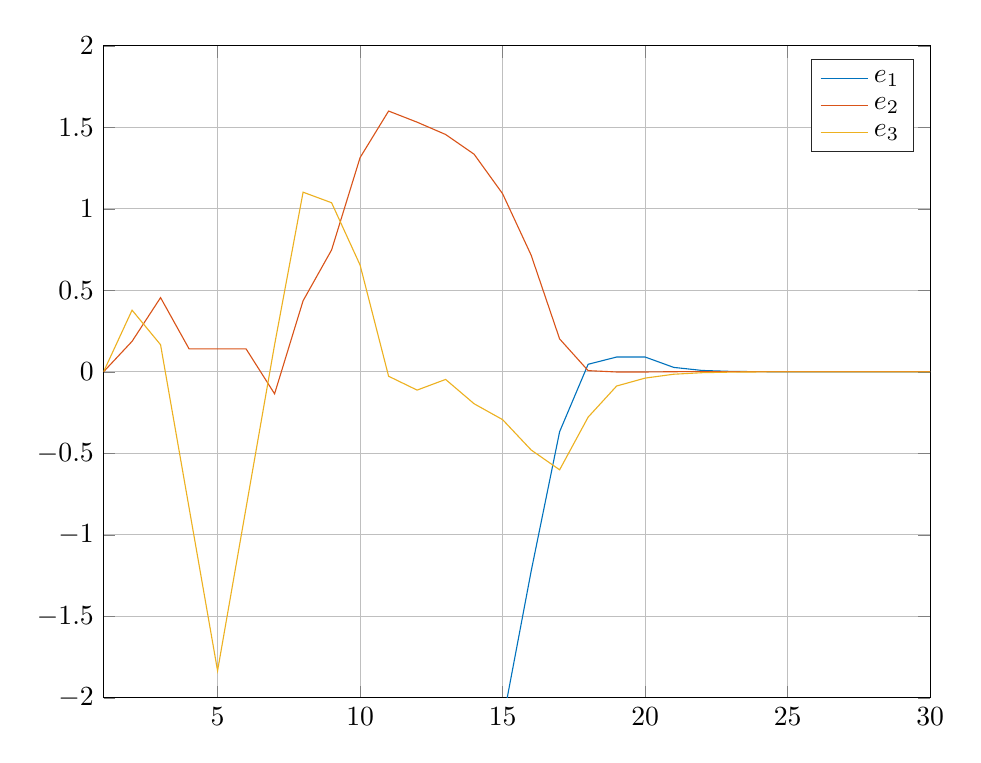
\begin{tikzpicture}

\begin{axis}[%
width=4.133in,
height=3.26in,
at={(0.693in,0.44in)},
scale only axis,
xmin=1,
xmax=30,
xmajorgrids,
ymin=-2,
ymax=2,
ymajorgrids,
axis background/.style={fill=white},
legend style={legend cell align=left,align=left,draw=white!15!black}
]
\addplot [color=mycolor1,solid]
  table[row sep=crcr]{%
1	-12\\
2	-11.023660576343\\
3	-10.06223352657\\
4	-9.15640740479144\\
5	-9.15640740479465\\
6	-9.15640740479465\\
7	-8.36219661717168\\
8	-7.58553726964379\\
9	-7.41462607590893\\
10	-6.91268483097867\\
11	-6.03250084804644\\
12	-5.05629656590124\\
13	-4.11081105067763\\
14	-3.1191097947464\\
15	-2.14933167101935\\
16	-1.22446146867001\\
17	-0.367530982776621\\
18	0.0459525429795825\\
19	0.0905373628765832\\
20	0.0905373628765832\\
21	0.0269727338482108\\
22	0.00812133374930781\\
23	0.00240494864695823\\
24	0.000657084699491795\\
25	0.000140507295145099\\
26	4.74406069501825e-06\\
27	-6.35056627392034e-05\\
28	-0.000101108809578609\\
29	-0.000116584360879211\\
30	-0.00012571920902496\\
};
\addlegendentry{$\text{e}_\text{1}$};

\addplot [color=mycolor2,solid]
  table[row sep=crcr]{%
1	0\\
2	0.18682288934014\\
3	0.454982392179511\\
4	0.140539352238494\\
5	0.140539352251824\\
6	0.140539352251825\\
7	-0.135158210900949\\
8	0.43571674789681\\
9	0.747551379744891\\
10	1.314156154839\\
11	1.59966987058902\\
12	1.53134064349713\\
13	1.45584838792566\\
14	1.33471535645463\\
15	1.09235312835811\\
16	0.715872380933145\\
17	0.201641958063727\\
18	0.0070297150644061\\
19	-0.0012164622450827\\
20	-0.00121646224508269\\
21	0.000494725068921926\\
22	0.000689549803282524\\
23	0.000711470322177271\\
24	0.000714059017782478\\
25	0.00071442325074535\\
26	0.00071448593376153\\
27	0.000714510822154342\\
28	0.000714522838832813\\
29	0.000714527463298887\\
30	0.000714529949604209\\
};
\addlegendentry{$\text{e}_\text{2}$};

\addplot [color=mycolor3,solid]
  table[row sep=crcr]{%
1	0\\
2	0.378129845761738\\
3	0.165880693074993\\
4	-0.834119306925007\\
5	-1.83411930692501\\
6	-0.834119306925008\\
7	0.165880693074995\\
8	1.10183360702685\\
9	1.03701890675625\\
10	0.654660876210552\\
11	-0.0273195696123133\\
12	-0.112442091712434\\
13	-0.0469097729122555\\
14	-0.196179442348173\\
15	-0.29361812975811\\
16	-0.479543046441075\\
17	-0.601419734911777\\
18	-0.27839119767171\\
19	-0.0873849630517223\\
20	-0.0387522133834468\\
21	-0.0150756512155249\\
22	-0.0055931370493166\\
23	-0.00207618930211248\\
24	-0.000885933368996808\\
25	-0.000524244077588615\\
26	-0.000399172515707895\\
27	-0.000330160599701867\\
28	-0.000308970913047415\\
29	-0.000288677060429233\\
30	-0.000255679062720028\\
};
\addlegendentry{$\text{e}_\text{3}$};

\end{axis}
\end{tikzpicture}%}
  \caption{The evolution of the error states of agent 1 over time.}
  \label{fig:d_OFF_3_1_errors_agent_1}
\end{figure}

\noindent\makebox[\linewidth][c]{%
\begin{minipage}{\linewidth}
  \begin{minipage}{0.45\linewidth}
    \begin{figure}[H]
      \scalebox{0.7}{% This file was created by matlab2tikz.
%
%The latest updates can be retrieved from
%  http://www.mathworks.com/matlabcentral/fileexchange/22022-matlab2tikz-matlab2tikz
%where you can also make suggestions and rate matlab2tikz.
%
\definecolor{mycolor1}{rgb}{0.00000,0.44700,0.74100}%
\definecolor{mycolor2}{rgb}{0.85000,0.32500,0.09800}%
\definecolor{mycolor3}{rgb}{0.92900,0.69400,0.12500}%
%
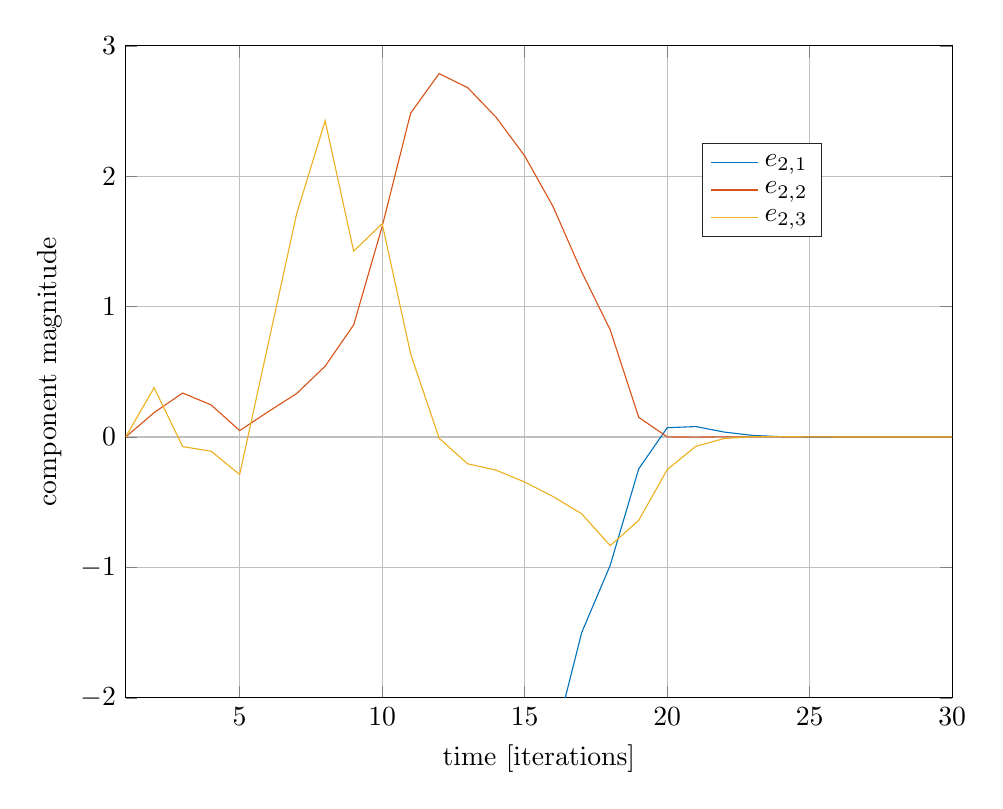
\begin{tikzpicture}

\begin{axis}[%
width=4.133in,
height=3.26in,
at={(0.693in,0.44in)},
scale only axis,
xmin=1,
xmax=30,
xmajorgrids,
ymin=-2,
ymax=3,
ymajorgrids,
xlabel={time [iterations]},
ylabel={component magnitude},
axis background/.style={fill=white},
legend style={at={(0.697,0.707)},anchor=south west,legend cell align=left,align=left,draw=white!15!black}
]
\addplot [color=mycolor1,solid]
  table[row sep=crcr]{%
1	-12\\
2	-11.0236602168649\\
3	-10.0435927924377\\
4	-9.04782819039047\\
5	-8.06877523767258\\
6	-7.39723250513838\\
7	-7.34492285992581\\
8	-7.45890065372688\\
9	-7.57584565893912\\
10	-7.54541696206043\\
11	-7.14168697170585\\
12	-6.20673741037639\\
13	-5.21415406387893\\
14	-4.24060181502826\\
15	-3.28555935189998\\
16	-2.36549905168856\\
17	-1.49990526801513\\
18	-0.984307444019737\\
19	-0.244533719146323\\
20	0.0710505803987044\\
21	0.0799366713627908\\
22	0.0376859330126464\\
23	0.0120466550397839\\
24	0.00227704161954091\\
25	-0.000180416041967136\\
26	-0.000411661274190785\\
27	-0.000360198644580103\\
28	-0.000340890786117166\\
29	-0.000329139247053743\\
30	-0.000291509351710069\\
};
\addlegendentry{$\text{e}_\text{2,1}$};

\addplot [color=mycolor2,solid]
  table[row sep=crcr]{%
1	0\\
2	0.186821494045275\\
3	0.337262762896568\\
4	0.245911308485647\\
5	0.0489048000807212\\
6	0.193672458322987\\
7	0.333292147922408\\
8	0.54303053148771\\
9	0.859429949921198\\
10	1.61435059234412\\
11	2.48406174160692\\
12	2.78658742058106\\
13	2.67890103665535\\
14	2.45086587883381\\
15	2.15556502537193\\
16	1.7651198814814\\
17	1.26582225971512\\
18	0.821589240745408\\
19	0.151058683610472\\
20	0.000585124975161591\\
21	-0.000860583595174803\\
22	0.000906832137207404\\
23	0.00102620759781356\\
24	0.00100421589430317\\
25	0.00100016951302778\\
26	0.00100004989113989\\
27	0.00100005131664536\\
28	0.00100004903462864\\
29	0.00100004695362088\\
30	0.00100003935591628\\
};
\addlegendentry{$\text{e}_\text{2,2}$};

\addplot [color=mycolor3,solid]
  table[row sep=crcr]{%
1	0\\
2	0.37812695257274\\
3	-0.0735027989077125\\
4	-0.109465067928805\\
5	-0.28767454667197\\
6	0.71232545332803\\
7	1.71232545332803\\
8	2.42483487766193\\
9	1.42483487766193\\
10	1.63618709765792\\
11	0.636187097657919\\
12	-0.0103033167039217\\
13	-0.205833379097595\\
14	-0.254330915654052\\
15	-0.345423668518832\\
16	-0.457248595204458\\
17	-0.589163451879382\\
18	-0.833203106853344\\
19	-0.639475942168837\\
20	-0.250371265773733\\
21	-0.0721894285433239\\
22	-0.0114250103640505\\
23	0.00211315703198815\\
24	0.00238889753649955\\
25	0.000904243730536457\\
26	0.000130345186757932\\
27	-7.49455508633238e-05\\
28	-0.000161436615819062\\
29	-0.000192731077038417\\
30	-0.000211081074229426\\
};
\addlegendentry{$\text{e}_\text{2,3}$};

\end{axis}
\end{tikzpicture}%
}
      \caption{The evolution of the error states of agent 2 over time.}
      \label{fig:d_OFF_3_1_errors_agent_2}
    \end{figure}
  \end{minipage}
  \hfill
  \begin{minipage}{0.45\linewidth}
    \begin{figure}[H]
      \scalebox{0.7}{% This file was created by matlab2tikz.
%
%The latest updates can be retrieved from
%  http://www.mathworks.com/matlabcentral/fileexchange/22022-matlab2tikz-matlab2tikz
%where you can also make suggestions and rate matlab2tikz.
%
\definecolor{mycolor1}{rgb}{0.00000,0.44700,0.74100}%
\definecolor{mycolor2}{rgb}{0.85000,0.32500,0.09800}%
\definecolor{mycolor3}{rgb}{0.92900,0.69400,0.12500}%
%
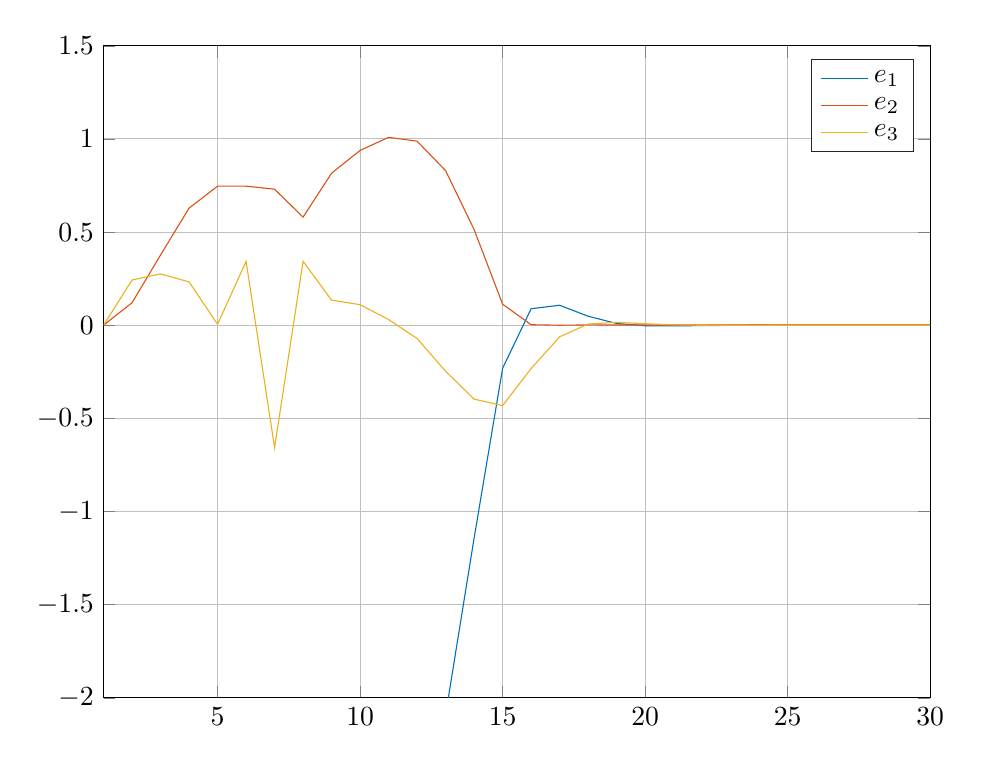
\begin{tikzpicture}

\begin{axis}[%
width=4.133in,
height=3.26in,
at={(0.693in,0.44in)},
scale only axis,
xmin=1,
xmax=30,
xmajorgrids,
ymin=-2,
ymax=1.5,
ymajorgrids,
axis background/.style={fill=white},
legend style={legend cell align=left,align=left,draw=white!15!black}
]
\addplot [color=mycolor1,solid]
  table[row sep=crcr]{%
1	-12\\
2	-11.0097917071458\\
3	-10.0432310216794\\
4	-9.07540049856288\\
5	-8.08457110014008\\
6	-8.08457110014008\\
7	-7.9828639800745\\
8	-7.03582268618902\\
9	-6.06593958449438\\
10	-5.07344272892607\\
11	-4.07617214081013\\
12	-3.07681024069303\\
13	-2.0907366103482\\
14	-1.14301010782759\\
15	-0.231328684393348\\
16	0.0884549332607789\\
17	0.107060387432856\\
18	0.0482307279955304\\
19	0.00938538074186046\\
20	-0.00310089626832872\\
21	-0.00367432377764027\\
22	-0.00199771731417777\\
23	-0.000848469212834647\\
24	-0.000218531715373383\\
25	-0.000137454581422754\\
26	-0.00026974349071711\\
27	-0.000349136109271304\\
28	-0.000368954513268945\\
29	-0.000361685464840086\\
30	-0.0003547125687542\\
};
\addlegendentry{$\text{e}_\text{1}$};

\addplot [color=mycolor2,solid]
  table[row sep=crcr]{%
1	0\\
2	0.120776119819851\\
3	0.377038740595294\\
4	0.628333925953931\\
5	0.746409484909325\\
6	0.746409484909326\\
7	0.730297368474817\\
8	0.580270117818618\\
9	0.816311755511841\\
10	0.938378998180139\\
11	1.00851475279787\\
12	0.98805288226454\\
13	0.829694408673164\\
14	0.513536877215149\\
15	0.112893835219851\\
16	0.00267984165032371\\
17	-8.2566438444481e-05\\
18	0.00156717222510608\\
19	0.00114848292315027\\
20	0.00100389671581321\\
21	0.00100104817911133\\
22	0.00100239141716044\\
23	0.0010016568708247\\
24	0.00100119474104185\\
25	0.00100115942266679\\
26	0.0010011853512981\\
27	0.00100119476951762\\
28	0.0010011975061209\\
29	0.00100119634074208\\
30	0.00100119516465476\\
};
\addlegendentry{$\text{e}_\text{2}$};

\addplot [color=mycolor3,solid]
  table[row sep=crcr]{%
1	0\\
2	0.242741836216831\\
3	0.275589436631646\\
4	0.232487057103612\\
5	0.0047310537811771\\
6	0.342888800307429\\
7	-0.657111199692569\\
8	0.342888800307433\\
9	0.134571500767573\\
10	0.110179468215538\\
11	0.0302447400635692\\
12	-0.0711888903013898\\
13	-0.247281780991812\\
14	-0.396691636915917\\
15	-0.431408875940715\\
16	-0.232395798495836\\
17	-0.0623966843494189\\
18	0.00632610914632695\\
19	0.0152297846325993\\
20	0.00792839860252519\\
21	0.00200664366583162\\
22	-0.000404314447867776\\
23	-0.000873993055716197\\
24	-0.00059323092067245\\
25	-0.000277998021568027\\
26	-0.000114002050335009\\
27	-0.000123254753909421\\
28	-0.00015291312141185\\
29	-0.000167728245259843\\
30	-0.000169602840944862\\
};
\addlegendentry{$\text{e}_\text{3}$};

\end{axis}
\end{tikzpicture}%}
      \caption{The evolution of the error states of agent 3 over time.}
      \label{fig:d_OFF_3_1_errors_agent_3}
    \end{figure}
  \end{minipage}
\end{minipage}
}


%-------------------------------------------------------------------------------
\subsection{Distances between actors}
\label{subsection:d_OFF_distances_3_1}


\noindent\makebox[\linewidth][c]{%
\begin{minipage}{\linewidth}
  \begin{minipage}{0.45\linewidth}
    \begin{figure}[H]\centering
      \scalebox{0.7}{% This file was created by matlab2tikz.
%
%The latest updates can be retrieved from
%  http://www.mathworks.com/matlabcentral/fileexchange/22022-matlab2tikz-matlab2tikz
%where you can also make suggestions and rate matlab2tikz.
%
\definecolor{mycolor1}{rgb}{0.00000,1.00000,1.00000}%
\definecolor{mycolor2}{rgb}{0.00000,0.44700,0.74100}%
%
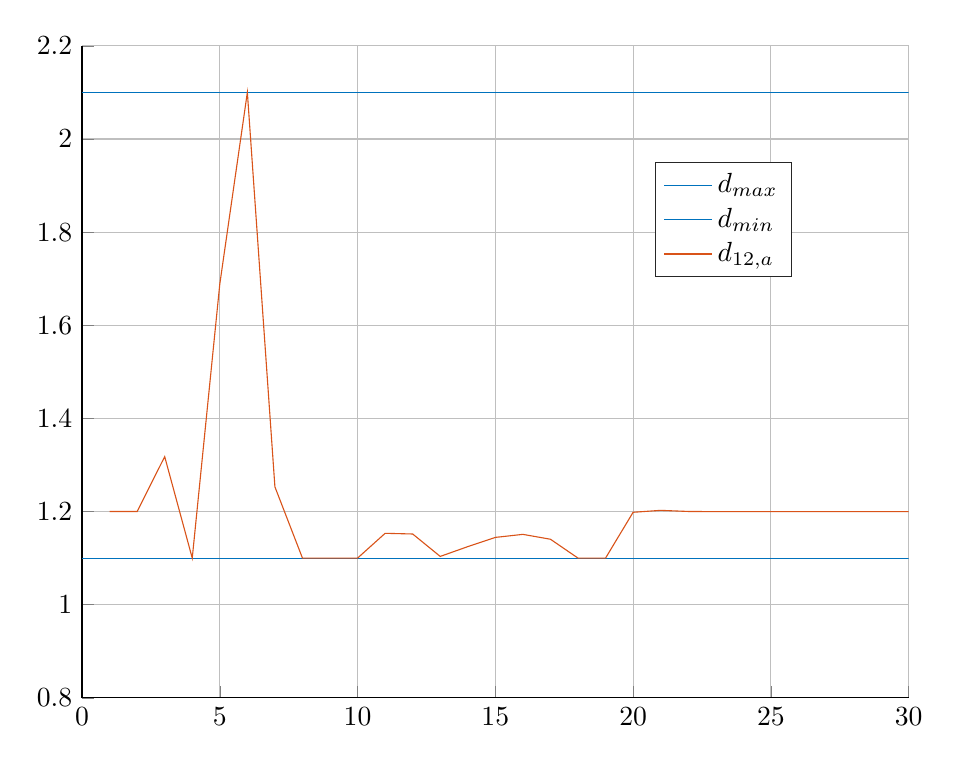
\begin{tikzpicture}

\begin{axis}[%
width=4.133in,
height=3.26in,
at={(0.693in,0.44in)},
scale only axis,
xmin=0,
xmax=30,
xmajorgrids,
ymin=0.8,
ymax=2.2,
ymajorgrids,
axis background/.style={fill=white},
axis x line*=bottom,
axis y line*=left,
legend style={at={(0.693,0.645)},anchor=south west,legend cell align=left,align=left,draw=white!15!black}
]
\addplot [color=mycolor1,solid]
  table[row sep=crcr]{%
0	1.1\\
30	1.1\\
};
\addlegendentry{$\text{d}_{\text{max}}$};

\addplot [color=mycolor1,solid]
  table[row sep=crcr]{%
0	2.1\\
30	2.1\\
};
\addlegendentry{$\text{d}_{\text{min}}$};

\addplot [color=mycolor2,solid]
  table[row sep=crcr]{%
1	1.2\\
2	1.20000139529492\\
3	1.31785147052563\\
4	1.09999999998642\\
5	1.68856849056261\\
6	2.09999999999301\\
7	1.2530007081749\\
8	1.10000000000969\\
9	1.09999999999727\\
10	1.1\\
11	1.15321392117776\\
12	1.15176661829333\\
13	1.10358381167611\\
14	1.12462219720809\\
15	1.14443187998148\\
16	1.15095311892003\\
17	1.1404904700737\\
18	1.10000000002504\\
19	1.1\\
20	1.19835686299168\\
21	1.20252224774948\\
22	1.20014692231401\\
23	1.19972400663661\\
24	1.19971093682928\\
25	1.19971429666118\\
26	1.19971450830707\\
27	1.19971449619204\\
28	1.19971449776632\\
29	1.19971449933898\\
30	1.19971450204907\\
};
\addlegendentry{$\text{d}_{\text{12,a}}$};

\end{axis}
\end{tikzpicture}%}
      \caption{The distance between agents 1 and 2 over time. The maximum allowed
        distance has a value of $2.1$ and the minimum allowed distance a value
        of $1.1$.}
      \label{fig:d_OFF_3_1_distance_agents_12}
    \end{figure}
  \end{minipage}
  \hfill
  \begin{minipage}{0.45\linewidth}
    \begin{figure}[H]
      \scalebox{0.7}{% This file was created by matlab2tikz.
%
%The latest updates can be retrieved from
%  http://www.mathworks.com/matlabcentral/fileexchange/22022-matlab2tikz-matlab2tikz
%where you can also make suggestions and rate matlab2tikz.
%
\definecolor{mycolor1}{rgb}{0.00000,0.44700,0.74100}%
%
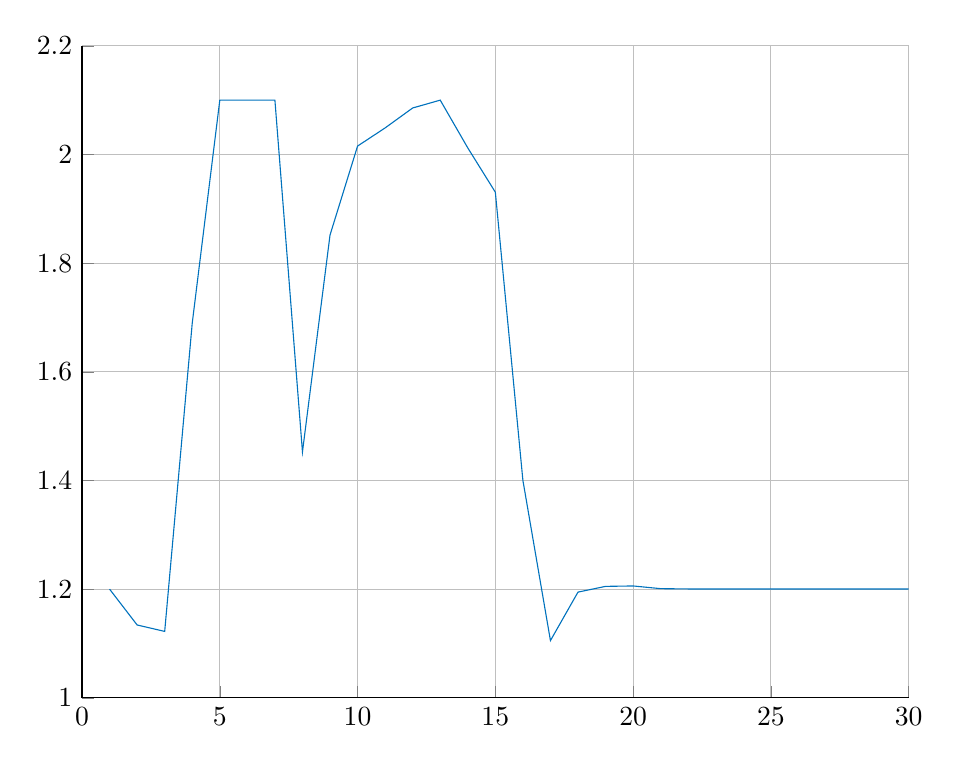
\begin{tikzpicture}

\begin{axis}[%
width=4.133in,
height=3.26in,
at={(0.693in,0.44in)},
scale only axis,
xmin=0,
xmax=30,
xmajorgrids,
ymin=1,
ymax=2.2,
ymajorgrids,
axis background/.style={fill=white},
axis x line*=bottom,
axis y line*=left
]
\addplot [color=mycolor1,solid,forget plot]
  table[row sep=crcr]{%
1	1.2\\
2	1.13403803924215\\
3	1.12221724466\\
4	1.68973744762907\\
5	2.1\\
6	2.1\\
7	2.09999999998609\\
8	1.45258730816118\\
9	1.85167711635705\\
10	2.01547880302627\\
11	2.04888118282851\\
12	2.08557835533293\\
13	2.1\\
14	2.01208243301112\\
15	1.9306407382238\\
16	1.40026104075947\\
17	1.10534650388814\\
18	1.19453962960084\\
19	1.20510045455713\\
20	1.20586148254091\\
21	1.20089744523363\\
22	1.20035549440056\\
23	1.20029459577754\\
24	1.20028745510684\\
25	1.20028676835707\\
26	1.20028673080313\\
27	1.20028671793289\\
28	1.20028670455237\\
29	1.20028669390253\\
30	1.20028668705898\\
};
\end{axis}
\end{tikzpicture}%}
      \caption{The distance between agents 1 and 3 over time. The maximum allowed
        distance has a value of $2.1$ and the minimum allowed distance a value
        of $1.1$.}
      \label{fig:d_OFF_3_1_distance_agents_13}
    \end{figure}
  \end{minipage}
\end{minipage}
}

\noindent\makebox[\linewidth][c]{%
\begin{minipage}{\linewidth}
  \begin{minipage}{0.45\linewidth}
    \begin{figure}[H]
      \scalebox{0.7}{% This file was created by matlab2tikz.
%
%The latest updates can be retrieved from
%  http://www.mathworks.com/matlabcentral/fileexchange/22022-matlab2tikz-matlab2tikz
%where you can also make suggestions and rate matlab2tikz.
%
\definecolor{mycolor1}{rgb}{0.00000,0.44700,0.74100}%
%
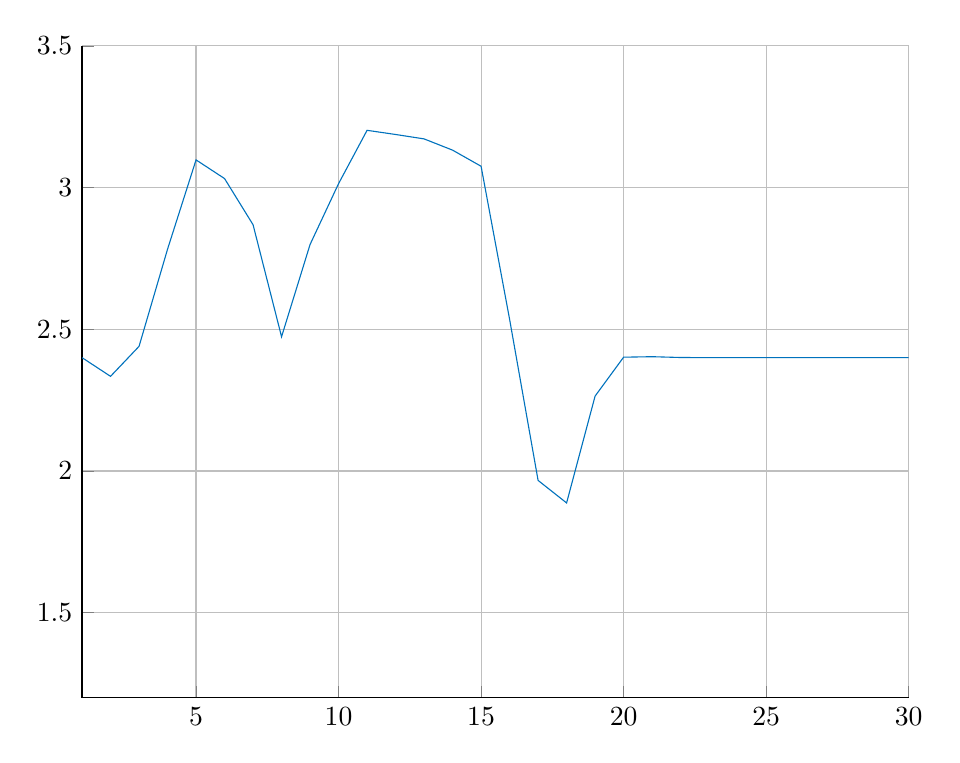
\begin{tikzpicture}

\begin{axis}[%
width=4.133in,
height=3.26in,
at={(0.693in,0.44in)},
scale only axis,
xmin=1,
xmax=30,
xmajorgrids,
ymin=1.2,
ymax=3.5,
ymajorgrids,
axis background/.style={fill=white},
axis x line*=bottom,
axis y line*=left
]
\addplot [color=mycolor1,solid,forget plot]
  table[row sep=crcr]{%
1	2.4\\
2	2.33399582920287\\
3	2.43977600452047\\
4	2.78255922746974\\
5	3.09754496041724\\
6	3.03168110004216\\
7	2.86883374850722\\
8	2.47368788811249\\
9	2.79905487605537\\
10	3.01379006458806\\
11	3.20187359968216\\
12	3.18719387378932\\
13	3.17160998984414\\
14	3.13195447560489\\
15	3.07506241378697\\
16	2.53542360623611\\
17	1.96685293835893\\
18	1.88744942730434\\
19	2.26437165992224\\
20	2.40156380744231\\
21	2.40331647868062\\
22	2.40042360548688\\
23	2.40001009192517\\
24	2.39999827632433\\
25	2.40000099029416\\
26	2.40000113965613\\
27	2.40000114347837\\
28	2.40000114863557\\
29	2.4000011496078\\
30	2.40000115664096\\
};
\end{axis}
\end{tikzpicture}%}
      \caption{The distance between agents 2 and 3 over time. The
        minimum allowed distance a value of $1.1$.}
      \label{fig:d_OFF_3_1_distance_agents_23}
    \end{figure}
  \end{minipage}
  \hfill
  \begin{minipage}{0.45\linewidth}
    \begin{figure}[H]
      \scalebox{0.7}{% This file was created by matlab2tikz.
%
%The latest updates can be retrieved from
%  http://www.mathworks.com/matlabcentral/fileexchange/22022-matlab2tikz-matlab2tikz
%where you can also make suggestions and rate matlab2tikz.
%
\definecolor{mycolor1}{rgb}{0.00000,0.44700,0.74100}%
\definecolor{mycolor2}{rgb}{0.85000,0.32500,0.09800}%
\definecolor{mycolor3}{rgb}{0.92900,0.69400,0.12500}%
\definecolor{mycolor4}{rgb}{0.00000,1.00000,1.00000}%
%
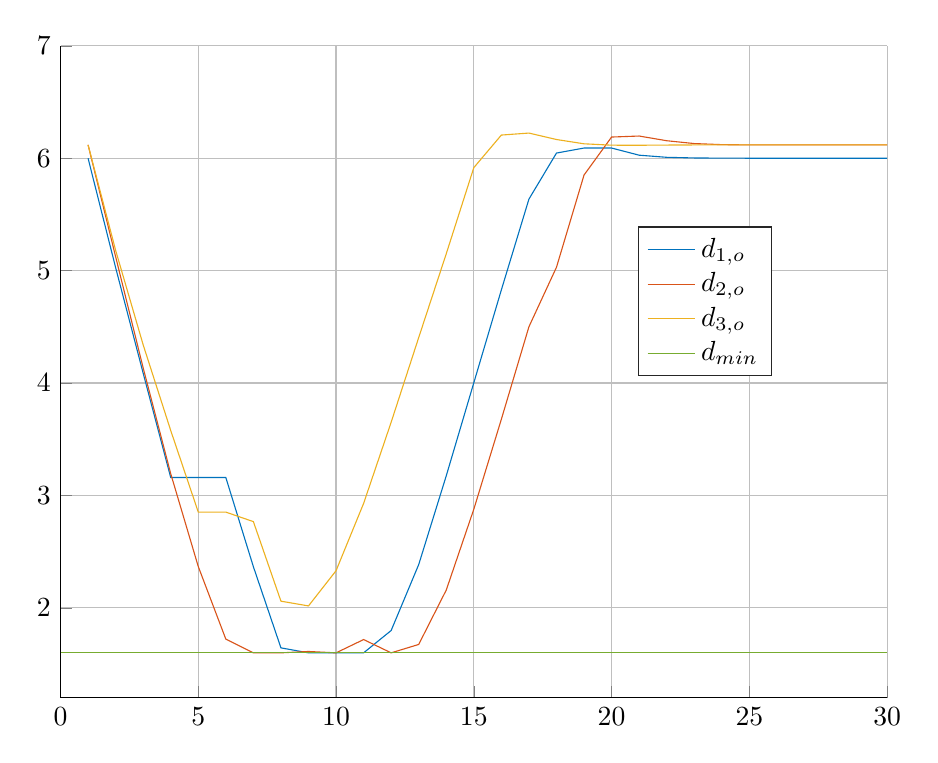
\begin{tikzpicture}

\begin{axis}[%
width=4.133in,
height=3.26in,
at={(0.693in,0.44in)},
scale only axis,
xmin=0,
xmax=30,
xmajorgrids,
ymin=1.2,
ymax=7,
ymajorgrids,
axis background/.style={fill=white},
axis x line*=bottom,
axis y line*=left,
legend style={at={(0.699,0.493)},anchor=south west,legend cell align=left,align=left,draw=white!15!black}
]
\addplot [color=mycolor1,solid]
  table[row sep=crcr]{%
1	6\\
2	5.02713321668369\\
3	4.08763381451694\\
4	3.15953461993216\\
5	3.15953461993596\\
6	3.15953461993596\\
7	2.36606014297002\\
8	1.64431673281861\\
9	1.6\\
10	1.59999999999993\\
11	1.59999999999814\\
12	1.79877189714427\\
13	2.38506381777668\\
14	3.17505802427009\\
15	4.00260939099088\\
16	4.82889651266211\\
17	5.63607724478942\\
18	6.04595662975308\\
19	6.09053748435851\\
20	6.09053748435851\\
21	6.02697275415301\\
22	6.00812137331899\\
23	6.00240499081256\\
24	6.00065712718486\\
25	6.00014054982753\\
26	6.00000478660151\\
27	5.99993653688152\\
28	5.99989893373638\\
29	5.99988345818574\\
30	5.99987432333795\\
};
\addlegendentry{$\text{d}_{\text{1,o}}$};

\addplot [color=mycolor2,solid]
  table[row sep=crcr]{%
1	6.11882341631134\\
2	5.12481147550222\\
3	4.13460496436342\\
4	3.19367216686597\\
5	2.36745668245154\\
6	1.72190411886172\\
7	1.60000000000124\\
8	1.60000000000064\\
9	1.61222749629448\\
10	1.6\\
11	1.71821526521605\\
12	1.5999999999985\\
13	1.67472448824822\\
14	2.15873745974645\\
15	2.87772350127174\\
16	3.67817313672458\\
17	4.50057609275879\\
18	5.02994696978362\\
19	5.85027093349297\\
20	6.1883964960392\\
21	6.19739429671976\\
22	6.15560523839159\\
23	6.13043580320701\\
24	6.12085946372372\\
25	6.11845042748196\\
26	6.11822368948176\\
27	6.11827415395476\\
28	6.11829308787901\\
29	6.11830461196345\\
30	6.11834151370955\\
};
\addlegendentry{$\text{d}_{\text{2,o}}$};

\addplot [color=mycolor3,solid]
  table[row sep=crcr]{%
1	6.11882341631134\\
2	5.18097119348033\\
3	4.33990417912756\\
4	3.57783358631378\\
5	2.85200746045381\\
6	2.85200746045381\\
7	2.76727257316978\\
8	2.05968209431013\\
9	2.01738968080501\\
10	2.33048774217713\\
11	2.92893343132289\\
12	3.65138518709042\\
13	4.40477010095544\\
14	5.15039410552641\\
15	5.91618618453318\\
16	6.20610363077024\\
17	6.22382426030142\\
18	6.16642997271828\\
19	6.12825181697869\\
20	6.11597982503738\\
21	6.1154170040195\\
22	6.11706123292011\\
23	6.11818797268868\\
24	6.11880556456414\\
25	6.11888505765971\\
26	6.11875534713459\\
27	6.11867750076947\\
28	6.11865806843129\\
29	6.11866519584543\\
30	6.11867203286652\\
};
\addlegendentry{$\text{d}_{\text{3,o}}$};

\addplot [color=mycolor4,solid]
  table[row sep=crcr]
      \caption{The distance between each agent and the obstacle over time. The
        minimum allowed distance has a value of $1.6$.}
      \label{fig:d_OFF_3_1_distance_obstacle_agents}
    \end{figure}
  \end{minipage}
\end{minipage}
}



%-------------------------------------------------------------------------------
\subsection{Input signals}
\label{subsection:d_OFF_inputs_3_1}

\begin{figure}[H]\centering
  \scalebox{0.7}{% This file was created by matlab2tikz.
%
%The latest updates can be retrieved from
%  http://www.mathworks.com/matlabcentral/fileexchange/22022-matlab2tikz-matlab2tikz
%where you can also make suggestions and rate matlab2tikz.
%
\definecolor{mycolor1}{rgb}{0.00000,1.00000,1.00000}%
\definecolor{mycolor2}{rgb}{0.00000,0.44700,0.74100}%
\definecolor{mycolor3}{rgb}{0.85000,0.32500,0.09800}%
%
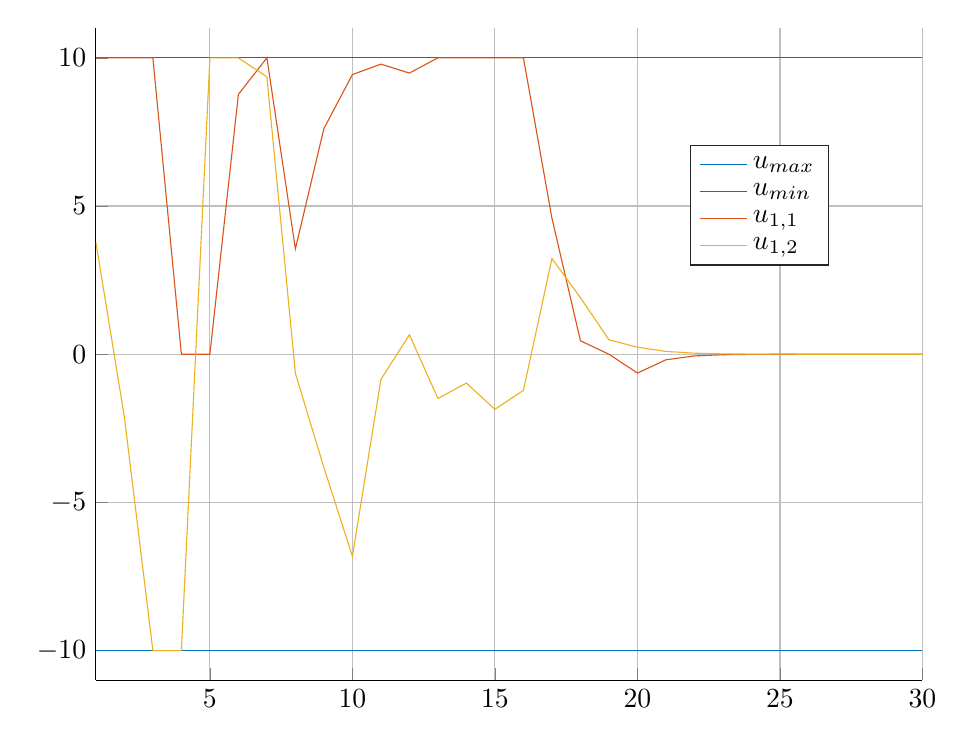
\begin{tikzpicture}

\begin{axis}[%
width=4.133in,
height=3.26in,
at={(0.693in,0.44in)},
scale only axis,
xmin=1,
xmax=30,
xmajorgrids,
ymin=-11,
ymax=11,
ymajorgrids,
axis background/.style={fill=white},
axis x line*=bottom,
axis y line*=left,
legend style={at={(0.719,0.636)},anchor=south west,legend cell align=left,align=left,draw=white!15!black}
]
\addplot [color=mycolor1,solid]
  table[row sep=crcr]{%
0	-10\\
30	-10\\
};
\addlegendentry{$\text{u}_{\text{max}}$};

\addplot [color=mycolor1,solid]
  table[row sep=crcr]{%
0	10\\
30	10\\
};
\addlegendentry{$\text{u}_{\text{min}}$};

\addplot [color=mycolor2,solid]
  table[row sep=crcr]{%
1	10\\
2	10\\
3	10\\
4	-1.43008982495135e-10\\
5	-5.55155180398176e-15\\
6	8.76780618849524\\
7	10\\
8	3.55662411622879\\
9	7.61589179520482\\
10	9.43511773832858\\
11	9.78888215281638\\
12	9.48664307072456\\
13	10\\
14	10\\
15	10\\
16	10\\
17	4.58985926575698\\
18	0.454099906611537\\
19	-4.01139935206858e-16\\
20	-0.635891430801749\\
21	-0.188524774380154\\
22	-0.0571643007739025\\
23	-0.0174786596765098\\
24	-0.00516577535570727\\
25	-0.00135763249009202\\
26	-0.000682497279857463\\
27	-0.00037603148760168\\
28	-0.000154755519918181\\
29	-9.13484848452184e-05\\
30	-0.000150190972100423\\
};
\addlegendentry{$\text{u}_{\text{1,1}}$};

\addplot [color=mycolor3,solid]
  table[row sep=crcr]{%
1	3.78129845761738\\
2	-2.12249152686745\\
3	-10\\
4	-10\\
5	10\\
6	10\\
7	9.35952913951856\\
8	-0.648147002706032\\
9	-3.82358030545695\\
10	-6.81980445822867\\
11	-0.85122522100121\\
12	0.655323188001785\\
13	-1.49269669435917\\
14	-0.974386874099374\\
15	-1.85924916682965\\
16	-1.21876688470703\\
17	3.23028537240067\\
18	1.91006234619988\\
19	0.486327496682754\\
20	0.236765621679221\\
21	0.094825141662081\\
22	0.0351694774720405\\
23	0.0119025593311565\\
24	0.00361689291408186\\
25	0.00125071561880717\\
26	0.000690119160060264\\
27	0.00021189686654452\\
28	0.000202938526181819\\
29	0.000329979977092037\\
30	-3.41053594282649e-06\\
};
\addlegendentry{$\text{u}_{\text{1,2}}$};

\end{axis}
\end{tikzpicture}%}
  \caption{The inputs signals directing agent 1 over time. Their value is
    constrained between $-10$ and $10$.}
  \label{fig:d_OFF_3_1_inputs_agent_1}
\end{figure}

\noindent\makebox[\linewidth][c]{%
\begin{minipage}{\linewidth}
  \begin{minipage}{0.45\linewidth}
    \begin{figure}[H]
      \scalebox{0.7}{% This file was created by matlab2tikz.
%
%The latest updates can be retrieved from
%  http://www.mathworks.com/matlabcentral/fileexchange/22022-matlab2tikz-matlab2tikz
%where you can also make suggestions and rate matlab2tikz.
%
\definecolor{mycolor1}{rgb}{0.00000,0.44700,0.74100}%
\definecolor{mycolor2}{rgb}{0.85000,0.32500,0.09800}%
%
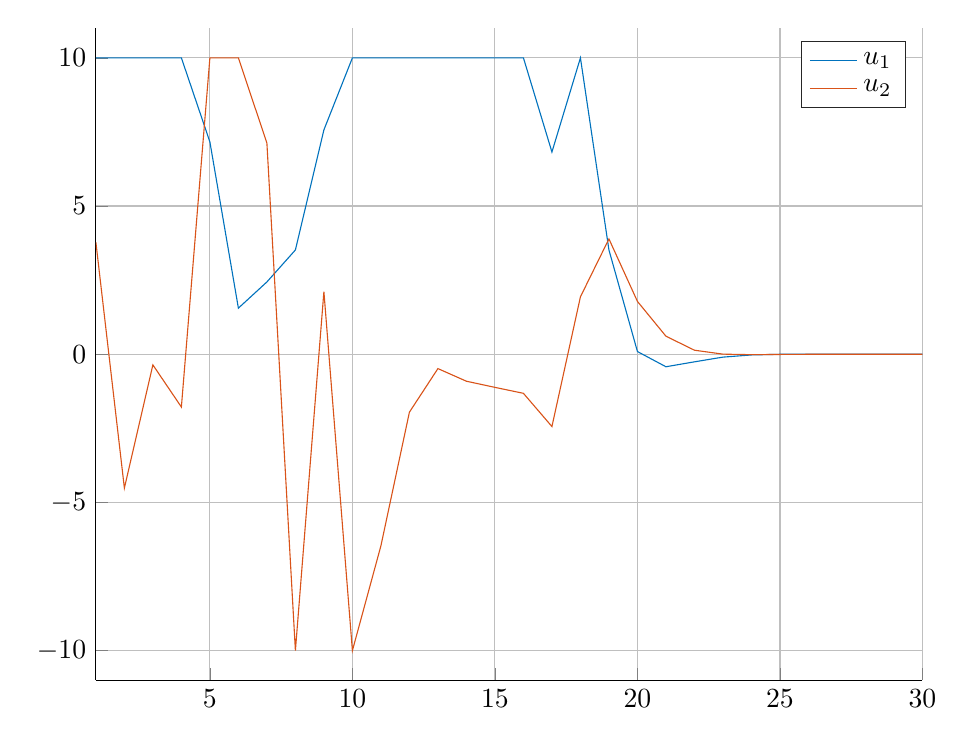
\begin{tikzpicture}

\begin{axis}[%
width=4.133in,
height=3.26in,
at={(0.693in,0.44in)},
scale only axis,
xmin=1,
xmax=30,
xmajorgrids,
ymin=-11,
ymax=11,
ymajorgrids,
axis background/.style={fill=white},
axis x line*=bottom,
axis y line*=left,
legend style={legend cell align=left,align=left,draw=white!15!black}
]
\addplot [color=mycolor1,solid]
  table[row sep=crcr]{%
1	10\\
2	10.0002392315268\\
3	10\\
4	10\\
5	7.16450842385731\\
6	1.55495615570192\\
7	2.43832329277864\\
8	3.51795940743551\\
9	7.56941704267642\\
10	10\\
11	10\\
12	10\\
13	10\\
14	10\\
15	10\\
16	10\\
17	6.82268063379982\\
18	10\\
19	3.51837632911962\\
20	0.0901484721492271\\
21	-0.422941956120491\\
22	-0.25639751678959\\
23	-0.0976963820316616\\
24	-0.0245746121853205\\
25	-0.00231245268934231\\
26	0.000514626297207931\\
27	0.000193078586038118\\
28	0.000117515392481582\\
29	0.00037629896111213\\
30	1.35562937325825e-05\\
};
\addlegendentry{$\text{u}_\text{1}$};

\addplot [color=mycolor2,solid]
  table[row sep=crcr]{%
1	3.7812695257274\\
2	-4.51629751480452\\
3	-0.359622690210924\\
4	-1.78209478743166\\
5	10\\
6	10\\
7	7.12509424333898\\
8	-10\\
9	2.1135221999599\\
10	-10\\
11	-6.46490414361842\\
12	-1.95530062393673\\
13	-0.484975365564568\\
14	-0.910927528647797\\
15	-1.11824926685626\\
16	-1.31914856674924\\
17	-2.44039654973962\\
18	1.93727164684507\\
19	3.89104676395104\\
20	1.7818183723041\\
21	0.607644181792721\\
22	0.135381673960384\\
23	0.00275740504511387\\
24	-0.0148465380596306\\
25	-0.00773898543778512\\
26	-0.00205290737621252\\
27	-0.00086491064955737\\
28	-0.000312944612193545\\
29	-0.000183499971910083\\
30	-0.000222306017977059\\
};
\addlegendentry{$\text{u}_\text{2}$};

\end{axis}
\end{tikzpicture}%}
      \caption{The inputs signals directing agent 2 over time. Their value is
        constrained between $-10$ and $10$.}
      \label{fig:d_OFF_3_1_inputs_agent_2}
    \end{figure}
  \end{minipage}
  \hfill
  \begin{minipage}{0.45\linewidth}
    \begin{figure}[H]
      \scalebox{0.7}{% This file was created by matlab2tikz.
%
%The latest updates can be retrieved from
%  http://www.mathworks.com/matlabcentral/fileexchange/22022-matlab2tikz-matlab2tikz
%where you can also make suggestions and rate matlab2tikz.
%
\definecolor{mycolor1}{rgb}{0.00000,1.00000,1.00000}%
\definecolor{mycolor2}{rgb}{0.00000,0.44700,0.74100}%
\definecolor{mycolor3}{rgb}{0.85000,0.32500,0.09800}%
%
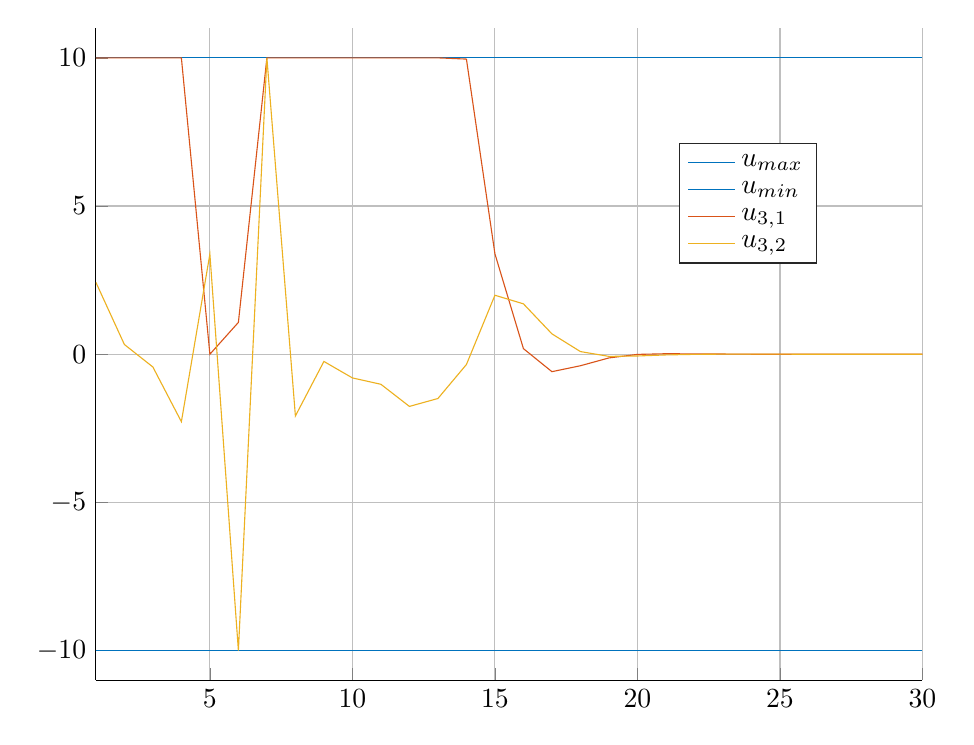
\begin{tikzpicture}

\begin{axis}[%
width=4.133in,
height=3.26in,
at={(0.693in,0.44in)},
scale only axis,
xmin=1,
xmax=30,
xmajorgrids,
ymin=-11,
ymax=11,
ymajorgrids,
axis background/.style={fill=white},
axis x line*=bottom,
axis y line*=left,
legend style={at={(0.705,0.639)},anchor=south west,legend cell align=left,align=left,draw=white!15!black}
]
\addplot [color=mycolor1,solid]
  table[row sep=crcr]{%
0	-10\\
30	-10\\
};
\addlegendentry{$\text{u}_{\text{max}}$};

\addplot [color=mycolor1,solid]
  table[row sep=crcr]{%
0	10\\
30	10\\
};
\addlegendentry{$\text{u}_{\text{min}}$};

\addplot [color=mycolor2,solid]
  table[row sep=crcr]{%
1	10\\
2	10\\
3	10\\
4	10\\
5	6.94025403719625e-14\\
6	1.07394599076332\\
7	10\\
8	10\\
9	10\\
10	10\\
11	10\\
12	10\\
13	10\\
14	9.95880251643974\\
15	3.38802366107827\\
16	0.188320763746648\\
17	-0.588643692988593\\
18	-0.388477319005367\\
19	-0.124871418451819\\
20	-0.00573435422274037\\
21	0.0167660740760852\\
22	0.0114924834665054\\
23	0.00629937669042249\\
24	0.000810771419789241\\
25	-0.00132288911983605\\
26	-0.000793926191131097\\
27	-0.000198184041873077\\
28	7.26904852234304e-05\\
29	6.97289618506946e-05\\
30	2.74947460858867e-05\\
};
\addlegendentry{$\text{u}_{\text{3,1}}$};

\addplot [color=mycolor3,solid]
  table[row sep=crcr]{%
1	2.42741836216831\\
2	0.328476004148146\\
3	-0.431023795280345\\
4	-2.27756003322435\\
5	3.38157746526253\\
6	-10\\
7	10\\
8	-2.0831729953986\\
9	-0.243920325520349\\
10	-0.799347281519691\\
11	-1.01433630364959\\
12	-1.76092890690422\\
13	-1.49409855924106\\
14	-0.347172390247975\\
15	1.99013077444878\\
16	1.69999114146417\\
17	0.687227934957458\\
18	0.0890367548627238\\
19	-0.0730138603007414\\
20	-0.0592175493669359\\
21	-0.0241095811369935\\
22	-0.00469678607848411\\
23	0.00280762135043742\\
24	0.00315232899104416\\
25	0.00163995971233015\\
26	-9.25270357441196e-05\\
27	-0.000296583675024278\\
28	-0.000148151238479933\\
29	-1.8745956850191e-05\\
30	1.2958095922861e-05\\
};
\addlegendentry{$\text{u}_{\text{3,2}}$};

\end{axis}
\end{tikzpicture}%}
      \caption{The inputs signals directing agent 3 over time. Their value is
        constrained between $-10$ and $10$.}
      \label{fig:d_OFF_3_1_inputs_agent_3}
    \end{figure}
  \end{minipage}
\end{minipage}
}
